\RequirePackage[l2tabu, orthodox]{nag} %编译时,给出过时命令和不规范使用警告。

\documentclass[UTF8, fontset = sourcesans, a4paper, oneside, zihao =
-4, scheme=chinese, no-math, space=true]{ctexbook}

\XeTeXgenerateactualtext=1

\usepackage[backend=biber,style=gb7714-2015,backref=true]{biblatex}
\addbibresource[location=local]{ref/refs.bib}

\usepackage{verse}

\ctexset{%
  abstractname = {摘\quad 要},  % book类没有摘要
  bibname = {参考文献},
  today = {big}
}
\xeCJKsetup{CJKmath=true}

\newcommand{\tightlist}{%
  \setlength{\itemsep}{0pt}\setlength{\parskip}{0pt}}

% 插图所需的宏包
\usepackage{graphicx}
\makeatletter
\def\maxwidth{\ifdim\Gin@nat@width>\linewidth\linewidth
\else\Gin@nat@width\fi}
\makeatother
\let\Oldincludegraphics\includegraphics
\renewcommand{\includegraphics}[1]{\Oldincludegraphics[width=\maxwidth]{#1}}


\usepackage{caption}
\captionsetup{font=small, labelfont=bf}

\usepackage{amsmath, amssymb, xfrac}
\usepackage[math-style=ISO, bold-style=ISO]{unicode-math} %注意,unicode-math与被其认为过时的bm包不兼容,不要\usepackage{bm}


\setmainfont[Scale=1.15]{Libertinus Serif}
\setmathfont[AutoFakeBold,Scale = 1.18]{Libertinus Math}  % 因Libertinus目前的数学字体暂还没
                                % 有粗体,这里设置为允许伪粗体渲染。

\setsansfont{TeX Gyre Heros}
\defaultfontfeatures{Scale=MatchLowercase}

\usepackage{etoolbox}
\usepackage{zref-perpage}
\zmakeperpage{footnote}

% % for number of footnote 
% 作者:刘海洋
% 链接:https://www.zhihu.com/question/53030087/answer/136097745
% 来源:知乎
% 著作权归作者所有。商业转载请联系作者获得授权,非商业转载请注明出处。

\makeatletter

% 无上标的 \@makefnmark
\def\nosuper@makefnmark{\hbox{\normalfont\@thefnmark\space}}

% 补丁
\patchcmd\@makefntext{\@makefnmark}{\nosuper@makefnmark}{}{}

%% 不用 etoolbox 的另一种打临时热补丁的写法
% \let\save@makefntext\@makefntext
% \long\def\@makefntext#1{{%
%   \let\@makefnmark\nosuper@makefnmark
%   \save@makefntext{#1}}}

% XeTeX 或 LuaTeX 下带圈数字 \thefootnote 的一种定义
\usepackage{xunicode-addon}
\newfontfamily\fnmarkfont{ipam.ttf}
\renewcommand\thefootnote{{\fnmarkfont\textcircled{\arabic{footnote}}}}
\makeatother

\AtBeginEnvironment{quotation}{\kaishu}


\usepackage{fancyhdr, geometry}

\geometry{%
  a4paper,
  heightrounded,
  % scale=0.7
  % margin=0cm,
  % marginparsep = 0.5cm,
  % marginparwidth=1cm,
  top = 3cm,
  bottom = 3cm,
  left = 2.6cm,
  right = 2.6cm,
  headheight = 6mm,
  headsep = 5mm,
  footskip = 6mm,
  % outer = 2.5cm,
  % inner = 2.5cm
}

% \pagestyle{headings}
% \fancyhf{} % clear all header and footer fields
% \lhead{}
% \rhead{}
% \chead{\slshape \zihao{5} \leftmark}
\pagestyle{fancy}
\fancyhead[LE,RO]{\slshape \zihao{5} \rightmark}
\fancyhead[LO,RE]{\slshape \zihao{5} \leftmark}
\fancyfoot[C]{\zihao{5} \thepage}
\renewcommand{\headrulewidth}{0.75pt}
\renewcommand{\footrulewidth}{0pt}
\fancyheadoffset{0cm}

\renewcommand{\bibfont}{\zihao{5}}
\setlength\parskip{0em plus 4pt minus 2pt}

% \usepackage{footnotebackref}  %bug
\usepackage{hyperref}

% for format of contents

\usepackage{bookmark}
\usepackage{booktabs}
\usepackage{lscape}

\usepackage{float} %允许浮动体强制在下方
% 双栏排版
% \usepackage{multicol}
% 有时候, 浮动的边注在双面模式下会出现在错误的一侧, mparhack 可以修正该问题
% \usepackage{mparhack}


% for format of contents
\usepackage{tocloft}
\usepackage{tocbibind}
% \renewcommand\cftsecleader{\cftdotfill{\cftdotsep}} % ctexart的目录中,section也加点。
% \renewcommand{\cftchapleader}{\cftdotfill{\cftdotsep}} % ctexbook中,chapter也加点。

\renewcommand{\cfttoctitlefont}{\hfill\Large\bfseries}
\renewcommand{\cftaftertoctitle}{\hfill} %使“目录”居中显示,将其中的toc改为lof
                                %和lot,则会使浮动体列表和表格列表也居中显示

% \renewcommand{\contentsname}{\hspace{\fill}\bfseries\Large
% 目录 \hspace{\fill}}   % 不使用tocloft宏包时也适用的命令。

% 设置目录中各级缩进
\settowidth{\cftsecindent}{2em}
\settowidth{\cftsubsecindent}{4em}
% 设置目录中 chapter 章节编号的宽度 (ctex 章节编号为中文, 需要特别注意).
% 参考 <<LaTeX 入门>>, 刘海洋 编著, 电子工业出版社, 2013.6
% \settowidth\cftchapnumwidth{第十章} % 最宽的可能编号
% \renewcommand\cftchapaftersnumb{\hspace{0.5em}} % 额外间距

\usepackage{enumitem}
\setenumerate[1]{itemsep=0pt,partopsep=0pt,parsep=\parskip,topsep=5pt}
\setitemize[1]{itemsep=0pt,partopsep=0pt,parsep=\parskip,topsep=5pt}
\setdescription{itemsep=0pt,partopsep=0pt,parsep=\parskip,topsep=5pt}
\setcounter{secnumdepth}{-2}
\hypersetup{
  pdftitle={列斐伏尔空间批判理论研究},
  pdfauthor={张笑夷 著},
  pdfborder={0 0 0},
  breaklinks=true,
  colorlinks}
\urlstyle{same}  % don't use monospace font for urls
% set default figure placement to htbp
\makeatletter
\def\fps@figure{htbp}
\makeatother

\title{列斐伏尔空间批判理论研究}
\author{张笑夷 著}
\date{2014-10-31T16:00:00+00:00}

\begin{document}
\maketitle

\protect\hypertarget{titlepage.xhtml}{}{}

\protect\hypertarget{part0000.html}{}{}

\begin{figure}[!tbp]
  \centering
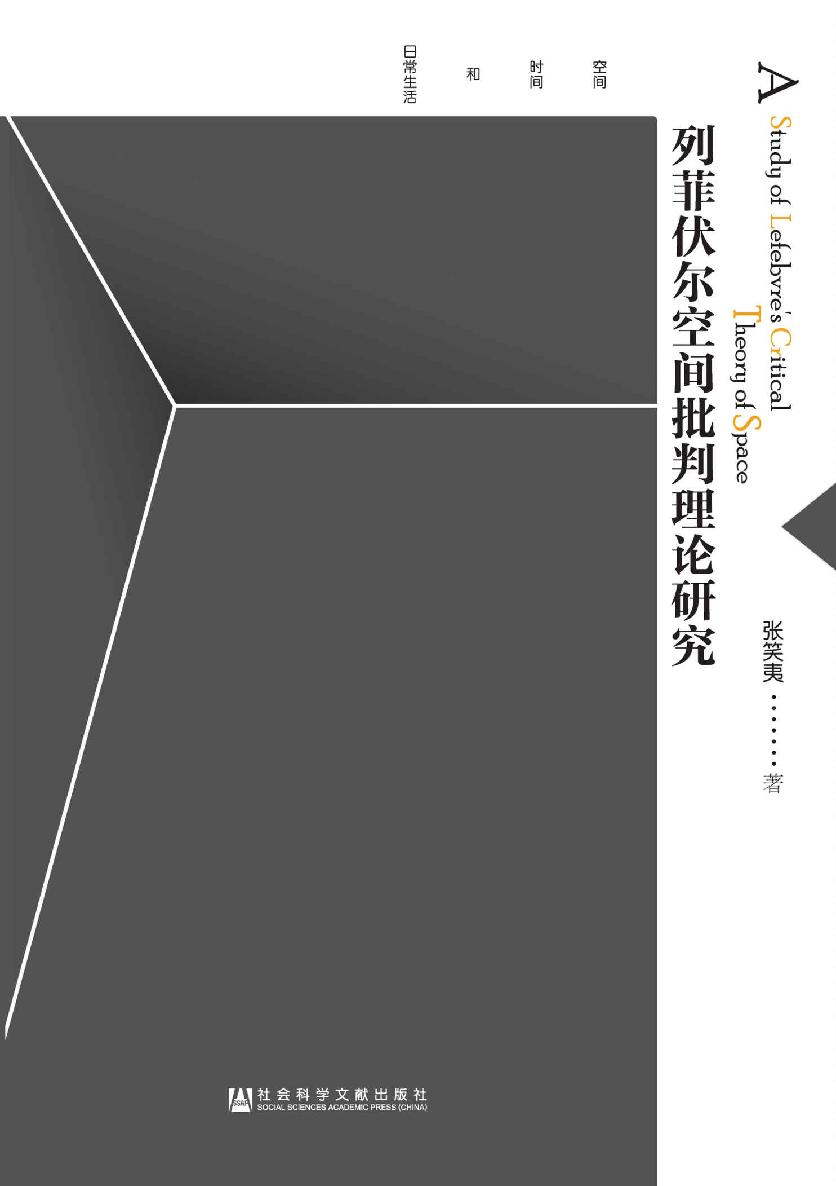
\includegraphics{images/00001.jpeg}
\end{figure}

\protect\hypertarget{part0001.html}{}{}

\begin{figure}[!tbp]
  \centering
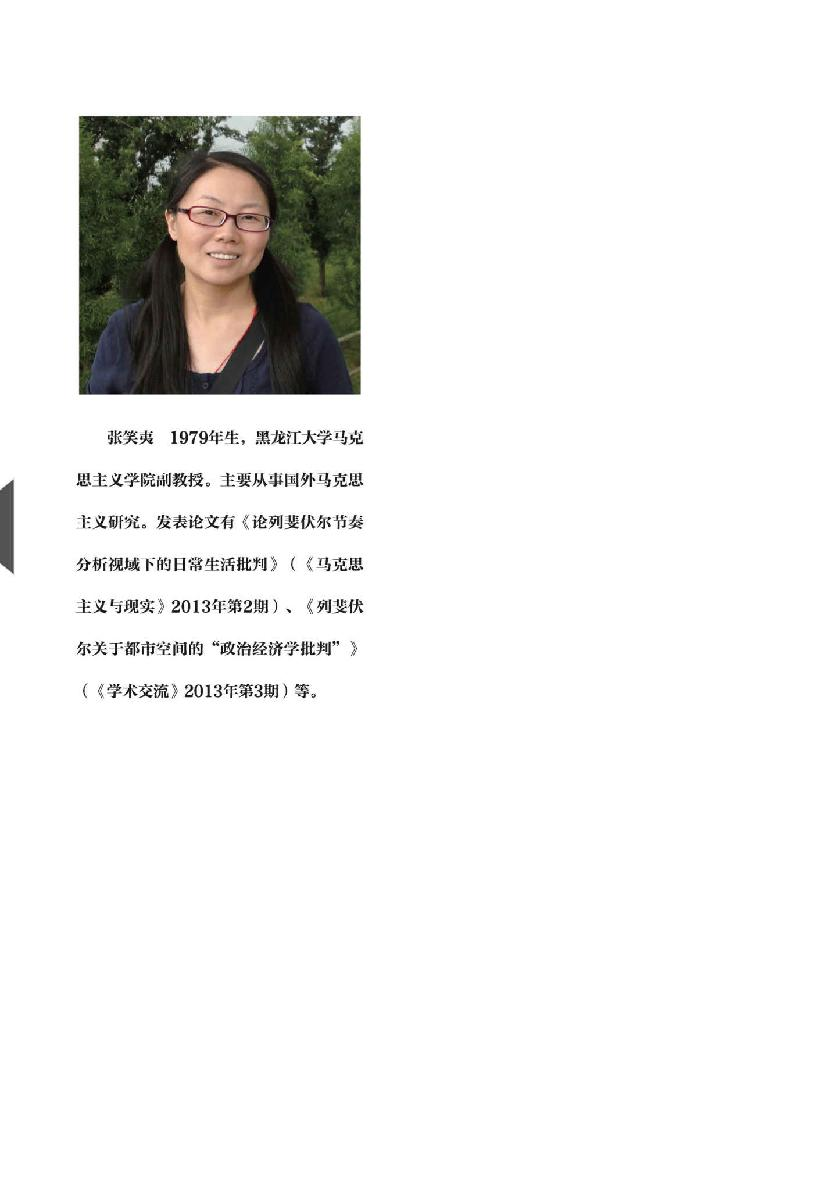
\includegraphics{images/00002.jpeg}
\end{figure}

\protect\hypertarget{part0002.html}{}{}

\begin{figure}[!tbp]
  \centering
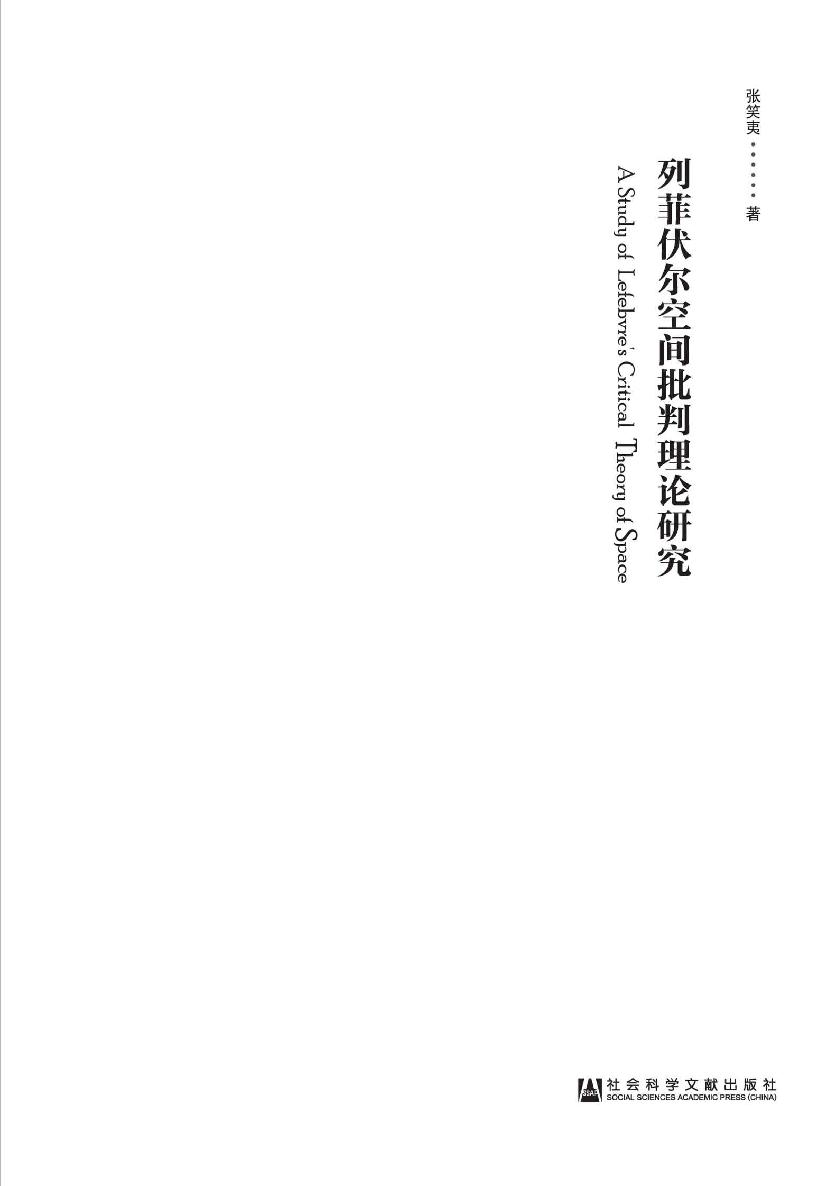
\includegraphics{images/00003.jpeg}
\end{figure}

\protect\hypertarget{part0003.html}{}{}

\begin{itemize}
\tightlist
\item
  \protect\hyperlink{part0004.htmlux5cux23a004}{导论}
\item
  \protect\hyperlink{part0005_split_000.htmlux5cux23a005}{第一章
  列斐伏尔空间批判的理论视域与方法}

  \begin{itemize}
  \tightlist
  \item
    \protect\hyperlink{part0005_split_001.htmlux5cux23b001}{第一节
    理论缘起:理论危机与现实契机}
  \item
    \protect\hyperlink{part0005_split_002.htmlux5cux23b002}{第二节
    理论视域:现代性批判}
  \item
    \protect\hyperlink{part0005_split_003.htmlux5cux23b003}{第三节
    研究范式:三元辩证法}
  \end{itemize}
\item
  \protect\hyperlink{part0006_split_000.htmlux5cux23a006}{第二章
  列斐伏尔对空间概念的考察}

  \begin{itemize}
  \tightlist
  \item
    \protect\hyperlink{part0006_split_001.htmlux5cux23b004}{第一节
    历史中的空间:空间概念历史变迁的批判性分析}
  \item
    \protect\hyperlink{part0006_split_002.htmlux5cux23b005}{第二节
    社会空间:一个生产性的总体性概念}
  \item
    \protect\hyperlink{part0006_split_003.htmlux5cux23b006}{第三节
    空间的历史:人类``史前史''的空间图绘}
  \end{itemize}
\item
  \protect\hyperlink{part0007_split_000.htmlux5cux23a007}{第三章
  资本主义的幸存与``空间的生产''}

  \begin{itemize}
  \tightlist
  \item
    \protect\hyperlink{part0007_split_001.htmlux5cux23b007}{第一节
    资本界限的激活:从``空间中物的生产''转向``空间本身的生产''}
  \item
    \protect\hyperlink{part0007_split_002.htmlux5cux23b008}{第二节
    国家和政治权力是空间生产的``管理者''}
  \item
    \protect\hyperlink{part0007_split_003.htmlux5cux23b009}{第三节
    空间生产的微观机制之一:都市化}
  \item
    \protect\hyperlink{part0007_split_004.htmlux5cux23b010}{第四节
    空间生产的微观机制之二:日常生活的被规划}
  \end{itemize}
\item
  \protect\hyperlink{part0008_split_000.htmlux5cux23a008}{第四章
  空间的矛盾性与总体性革命}

  \begin{itemize}
  \tightlist
  \item
    \protect\hyperlink{part0008_split_001.htmlux5cux23b011}{第一节
    矛盾性的空间:资本主义的``阿喀琉斯之踵''}
  \item
    \protect\hyperlink{part0008_split_002.htmlux5cux23b012}{第二节
    ``试验性的乌托邦'':探索另一个可能的世界}
  \item
    \protect\hyperlink{part0008_split_003.htmlux5cux23b013}{第三节
    对革命的再思考}
  \end{itemize}
\item
  \protect\hyperlink{part0009_split_000.htmlux5cux23a009}{第五章
  从空间分析走向节奏分析}

  \begin{itemize}
  \tightlist
  \item
    \protect\hyperlink{part0009_split_001.htmlux5cux23b014}{第一节
    节奏概念与节奏分析方法的内涵}
  \item
    \protect\hyperlink{part0009_split_002.htmlux5cux23b015}{第二节
    时间与空间的节奏化组织}
  \item
    \protect\hyperlink{part0009_split_003.htmlux5cux23b016}{第三节
    线性重复的社会时间生产的微观权力机制}
  \item
    \protect\hyperlink{part0009_split_004.htmlux5cux23b017}{第四节
    反抗线性重复的持久努力}
  \end{itemize}
\item
  \protect\hyperlink{part0010_split_000.htmlux5cux23a010}{第六章
  列斐伏尔空间批判的理论启示}

  \begin{itemize}
  \tightlist
  \item
    \protect\hyperlink{part0010_split_001.htmlux5cux23b018}{第一节
    空间批判与经典西方马克思主义的文化批判}
  \item
    \protect\hyperlink{part0010_split_002.htmlux5cux23b019}{第二节
    空间批判对马克思主义社会历史理论的丰富和发展}
  \end{itemize}
\item
  \protect\hyperlink{part0011.htmlux5cux23a011}{结语}
\item
  \protect\hyperlink{part0012.htmlux5cux23a012}{参考文献}
\item
  \protect\hyperlink{part0013.htmlux5cux23a013}{后记}
\end{itemize}

\protect\hypertarget{part0004.html}{}{}

\hypertarget{part0004.htmlux5cux23a004}{\chapter{导论}\label{part0004.htmlux5cux23a004}}

20世纪是一个风云变幻的时代。两次世界大战把人们从对理性的痴梦中惊醒,\textbf{启蒙运动所弘扬的理性精神走向了自己的反面。科学技术成为支配人、压抑人甚至消灭人的异化力量,由理性原则组织和规划的社会已然成为不适宜人居住的异化社会。}这也就不难想象学生造反运动为什么会在20世纪60、70年代出现,而且是在全球同时出现。然而,资本主义并没有因为运动、革命和经济危机等接踵而至的阻挠停住脚步,恰恰相反,在经历了一系列至关重要的生产关系变革后,它似乎显得更加牢不可破。当今,在被冠以``后工业时代''、``消费社会''、``信息社会''等一系列名号的资本主义社会面前,人们------包括曾经坚定的马克思主义者------更愿意重复``\textbf{别无选择}''这个口号,而不是``\textbf{改变现实}''。在资本主义虚假的强势面前,共产主义运动一再受挫。按照马克思的构想,当资本主义国家的生产关系不再适应生产力发展的要求时,无产阶级便可抓住时机,进行革命,推翻资本主义社会。事实上,历史的实际发展进程远比马克思的构想复杂,一些新的情况是马克思所未曾预见到的。虽然俄国社会主义革命取得了成功,但同时期的德国、奥地利、意大利、匈牙利等资本主义国家的无产阶级革命却均以失败收场。更令人扼腕的是,苏联社会主义也未前行多远便轰然倒下。

这个时代需要马克思的学说,因为只有马克思对资本主义进行了最全面和最深刻的分析,对共产主义进行了最透彻的论证。诚如伊格尔顿所言:``只要资本主义制度还存在一天,马克思主义就不会消亡。只有在资本主义结束之后,马克思主义才会退出历史的舞台。''\protect\hypertarget{part0004.htmlux5cux23w1}{}{}\protect\hyperlink{part0004.htmlux5cux23m1}{\textsuperscript{{[}1{]}}}确实,马克思和恩格斯的思想在这个时代得到了积极的回应和前所未有的发展。这表现为导源于马克思和恩格斯学说的众多马克思主义理论相互并存。``一方面,它同当代哲学、社会学等领域的其他理论成果交汇形成了众多马克思主义流派;另一方面,它被运用于不同地区的实际革命进程,由此而导致了不同的马克思主义实践模型,即社会主义模式。这样,20世纪马克思主义的表述形态便呈现出多样化的格局。''\protect\hypertarget{part0004.htmlux5cux23w2}{}{}\protect\hyperlink{part0004.htmlux5cux23m2}{\textsuperscript{{[}2{]}}}在这些多样化的马克思主义形态中,不仅有长期占据主导地位的经典马克思主义,而且还包括西方马克思主义、东欧新马克思主义,以及欧洲共产主义、民主社会主义、后现代马克思主义等等。尽管这些马克思主义流派的主张和观点互不相同,甚至相互冲突,但他们大多秉承了马克思的批判精神,强调对现实社会的批判和变革。其中,西方马克思主义尤为典型。

西方马克思主义流派甚多,观点各异。\textbf{大体来说,西方马克思主义可分为人本主义的马克思主义和科学主义的马克思主义。人本主义的马克思主义}包括黑格尔主义的马克思主义、弗洛伊德主义的马克思主义、法兰克福学派、存在主义的马克思主义等,\textbf{强调``青年马克思''的哲学人类学思想,以此展开对资本主义理性文化的审查和批判。}比如,西方马克思主义的奠基人卢卡奇批判资本主义商品经济的物化结构对无产阶级革命意识的禁锢;法兰克福学派的代表人物\textbf{霍克海默}一针见血地指出,\textbf{启蒙理性依赖于神话,驱除了神话,却最终退化为神话,走向了自我毁灭;}法兰克福学派的另一位代表人物、弗洛伊德主义的马克思主义者\textbf{马尔库塞}认为,\textbf{发达资本主义社会是一个对人全方位控制因而全面压抑人的单向度社会;}等等。与人本主义的马克思主义相对立,科\textbf{学主义的马克思主义强调``老年马克思''思想的科学性,以此捍卫马克思。}比如,阿尔都塞关注科学方法论结构和客观规律,拒斥非历史的人和主体性,认为马克思主义既非人道主义也非历史主义。在传统西方马克思主义之后出现的生态学的马克思主义、女权主义的马克思主义、文化的马克思主义、后现代马克思主义尽管已经从根本上否定了历史唯物主义的基本观点,但它们仍试图在新的条件下激活马克思主义的批判精神,在批判中寻求解放之路。

无论西方马克思主义是以何种方式进入或发展马克思主义,无论是否偏离了经典马克思主义的本义,但有如下三点是值得肯定的。第一,西方马克思主义通过对20世纪资本主义意识形态、科学技术、市民社会、日常生活、社会空间、性格结构和心理机制、现代国家、现代性机制等的批判和分析,深刻揭示了资本主义的新变化、新特征以及新的存续机制。\textbf{结论表明,资本主义正试图强制性地调动一切资源和要素来维持自身的存在,尤其是通过把技术理性文化、大众文化、意识形态文化等整合成一个总体性的操控机制来维持自身。}第二,西方马克思主义准确地揭示了当代人的命运。在一个由理性原则或理性文化所构筑的同质性的社会中,无论是社会、自然、他人、自我、劳动等皆以陌生和敌对的样态出现,人处于一个总体异化的境遇中。可悲的是,大部分人并不自知自己的异化,反而盲目甚至麻木地接受并参与异化结构的生产和再生产。存在主义所言之``被抛''用以形容当代人的命运是再恰当不过。第三,西方马克思主义敏锐地意识到了20世纪出现的``文化危机'',并自觉地进行了深刻的理论反思,进而``实现了马克思主义哲学向实践哲学和文化哲学范式的回归,使马克思主义在20世纪历史条件下焕发出新的活力''\protect\hypertarget{part0004.htmlux5cux23w3}{}{}\protect\hyperlink{part0004.htmlux5cux23m3}{\textsuperscript{{[}3{]}}}。\textbf{当资本主义实现了外在的、物质的强力控制机制,向总体化的、文化的操纵机制转化时,如果马克思主义理论的视野还仅停留在经济主题上,忽略社会的政治和文化问题,那么它就注定被抛弃。}在重视社会的政治和文化问题方面,西方马克思主义表现得尤为出色。``在这里,关于人的自由和创造性的文化价值的形而上的思考和关于人的生存境遇的现实的文化批判有机地结合起来,关于马克思主义研究的`学术性'和`现实性'同样具有内在统一的特点。''\protect\hypertarget{part0004.htmlux5cux23w4}{}{}\protect\hyperlink{part0004.htmlux5cux23m4}{\textsuperscript{{[}4{]}}}\textbf{总体来说,西方马克思主义是一种在``文化焦虑的时代''诞生的``文化批判理论''},不仅揭示了社会的境况和人的遭遇,而且运用文化哲学范式大大拓展了马克思主义的视域。

在西方马克思主义阵营中,确切地说,在人本主义的马克思主义流派中,有这样一位思想家:他坚持不懈地对资本主义秩序下的日常生活进行精细的分析和激烈的批判,并满怀希望地呼唤着总体性革命的到来;他是一个马克思主义者,主张运用马克思的辩证唯物主义和历史唯物主义进行研究,但同时又率先颠覆了马克思学说中物质生产方式的基础性地位,代之以``空间的生产'';他因为日常生活批判而赢得理论界的认可,更因为空间批判理论而获得广泛的赞誉和关注;他像其他的西方马克思主义者一样从事着文化批判,但他关注的领域远远超过了政治和文化领域;他像其他的西方马克思主义者一样对人类思想文化进程产生着重要影响,但没有哪种思想像他的空间批判理论那样被社会学、哲学、人类学、地理学、建筑学、城市学等众多学科所追捧。他就是列斐伏尔。

\section{一 列斐伏尔的学术路径}\label{part0004.htmlux5cux23c001}

亨利·列斐伏尔(Henri
Lefebvre,1901---1991,又译亨利·勒菲弗、亨利·列斐伏尔等)是法国现代著名的哲学家和思想家、西方马克思主义的著名代表人物。在长达60年的学术生涯中,列斐伏尔为后世留下了60多部个人著作和发表在多家杂志和报纸上的文章,以及一些由他主持出版的马克思、黑格尔、列宁的著作。列斐伏尔以多变和挑衅的风格不断地介入20世纪的社会历史变迁,他的作品广泛地涉及了日常生活、空间、时间、历史、文学、建筑等领域,他的传奇一生\protect\hypertarget{part0004.htmlux5cux23w5}{}{}\protect\hyperlink{part0004.htmlux5cux23m5}{\textsuperscript{{[}5{]}}}和学术历险是对20世纪最好的注解。爱德华·索亚(E.W.Soja,又译爱德华·索杰)曾这样评价:``在1991年静静地`消失'的不是亨利·列斐伏尔,而是20世纪本身。''\protect\hypertarget{part0004.htmlux5cux23w6}{}{}\protect\hyperlink{part0004.htmlux5cux23m6}{\textsuperscript{{[}6{]}}}

日常生活批判贯穿列斐伏尔的整个学术生涯,是其最伟大的思想贡献。列斐伏尔正是因为关于现代日常生活研究的系列著作,而与卢卡奇、阿多诺、马尔库塞等人并驾齐驱,进入了20世纪社会批判理论大师的行列。无论时代如何变幻,日常永远是列斐伏尔对社会变革的社会学探究和哲学反思必不可少的最基本的领域。列斐伏尔认为自己采取定期更新系列著作来研究日常生活的方式,保证了理论与重大社会变化的历史分期的一致性。因此,分别出版于1947年、1961年和1981年的《日常生活批判》三卷本以及在他生命最后通过节奏分析方法对日常生活的再考察可以被视为列斐伏尔思想的界标和里程碑。本书根据前后跨越近半个世纪的日常生活批判系列著作对列斐伏尔的思想发展历程进行分期。\textbf{从总体上,我们可以把列斐伏尔的学术生涯划分为日常生活批判思想确立,以现代性为思考原点对都市、日常生活的社会学研究和政治经济学批判,以及从现代性到现代主义的社会变迁中对日常生活的再审视三个阶段。}

\textbf{第一个阶段是从其学术生涯的开端到《现代性导论》出版之前(时间上大约从20世纪20年代中后期到50年代末),这是列斐伏尔对马克思主义的译介、阐释和日常生活批判理论初步确立的阶段。}早在20世纪20年代中后期,列斐伏尔就开始将马克思主义介绍到法国学术界。1928年,他与一批年轻的哲学家创办了法国第一个马克思主义哲学刊物《马克思主义杂志》。从30年代到40年代,列斐伏尔在大学教授哲学,并积极参与反法西斯抵抗运动。二战后,他重新活跃于法国思想界。列斐伏尔遵循既要坚持马克思主义又要超越马克思主义的原则,与东欧新马克思主义者和法国的非共产信仰的知识分子联合在一起,形成了一股强大的反斯大林主义的势力。这一时期的主要著作有:与古特曼合著的《被神秘化的意识》(1936年),《反民族的民族主义》(1937年),与古特曼合著的《列宁论黑格尔辩证法的笔记》、《黑格尔文选》、《希特勒掌权,或法西斯德国五年总结》(1938年),《尼采》、《辩证唯物主义》(1939年),《存在主义》(1946年),《笛卡尔》、《马克思主义与自由》、《形式逻辑,辩证逻辑》、《日常生活批判Ⅰ:导论》(1947年),《马克思主义》、《论对马克思思想的理解》(1948年),《美学概论》(1953年),《论对列宁思想的理解》、《马克思主义的现实问题》、《论德国》(1957年),《总结及其他》(1959年)。其中,《被神秘化的意识》、《辩证唯物主义》和《日常生活批判Ⅰ:导论》是列斐伏尔的代表作。在这一思想阶段,他因日常生活批判以及异化、人道主义、青年马克思思想等方面的研究得到西方学界的广泛关注,与卢卡奇、葛兰西、阿多诺等人齐名,被誉为杰出的西方马克思主义哲学家、日常生活批判理论家、``现代法国辩证法之父''。

\textbf{第二个阶段是以《现代性导论》为界标到《日常生活批判Ⅲ:从现代性到现代主义(走向日常的元哲学)》出版之前(时间上大约从60年代初到70年代末),这是列斐伏尔以现代性问题为思考原点对当代新资本主义进行社会学和政治经济学批判的阶段。}这一阶段以1968年学生运动为界标又可以分为\textbf{两个时期}。

\textbf{第一个时期从60年代初到1968年学生运动之前,是列斐伏尔现代性思想确立和从事城市和日常生活批判的社会学研究时期。}这一时期的主要著作(含编著)有《现代性导论》、《日常生活批判Ⅱ:日常性的社会学基础》(1962年),《乡村的谷底------乡村社会学研究》、与古特曼合编的《卡尔·马克思文集》(第一卷)(1963年),《作为哲学家的马克思》、《卡尔·马克思文集》(第二卷)(1964年),《元哲学》、《比利牛斯山》、《公社宣言》(1965年),《马克思的社会学》、《语言与社会》(1966年),《立场:反对技术官僚论》(1967年),《爆炸:马克思主义与法国革命》、《城市的权利》、《现代世界中的日常生活》(1968年)。其中,《现代性导论》、《日常生活批判Ⅱ:日常性的社会学基础》、《马克思的社会学》、《城市的权利》和《现代世界中的日常生活》是列斐伏尔的代表作。其实,从50年代开始,列斐伏尔就有了除马克思主义者之外的另一个``乡村社会学家''的身份。在这一思想时期,他凭借马克思主义思想框架,在城市社会学、乡村社会学、社会语言学以及日常社会学等领域进行了卓有成效的研究,被法国社会学界公认为这些领域的奠基人。\textbf{这一时期的日常生活批判思想以《现代世界中的日常生活》为其研究顶峰。}列斐伏尔在对日常生活的社会学基础进行批判性分析的基础上,把当时的西方社会定义为``消\textbf{费受控的官僚社会''(Bureaucratic
Society of Controlled
Consumption)}。列斐伏尔认为,\textbf{在这种社会中,现代性作为一种全方位的工具理性主义通过``技术专家治国制''(technocracy)隐蔽地``规划''日常生活。``日常生活已不再是富有潜在主体性的`主体';它已经变成社会组织系统的`客体'。''}\protect\hypertarget{part0004.htmlux5cux23w7}{}{}\protect\hyperlink{part0004.htmlux5cux23m7}{\textsuperscript{{[}7{]}}}

\textbf{第二个时期从1968年学生运动到70年代末,是列斐伏尔以空间、国家、都市和日常生活为主题进行资本主义政治经济学批判时期。}根据列斐伏尔的权威研究专家米歇尔·特雷比奇(Michel
Trebitsch)的观点,列斐伏尔对空间和城市问题的研究深受1968年学生运动的影响。作为南泰尔学院的社会学教授,列斐伏尔在1968年的反抗运动中对学生的影响无疑是巨大的。他提出的``改造生活''、``不要改变雇主,而要改变生活的被雇佣''、``让日常生活成为一件艺术品''等在``五月风暴''中成为最流行的口号。列斐伏尔将学生视为社会解放、实现``总体人''这一终极目标的代言人。1968年2月,列斐伏尔远赴日本,与全日本学生自治团体联合会(Zengakuren)取得了联系。5月,在南泰尔学院,列斐伏尔不仅站在反抗运动的最前线,积极保护学生并与运动的领导人一起参加电视访谈,而且透过反抗运动现象冷静思考背后的深层社会问题。列斐伏尔发现,\textbf{``当经济的和社会的`基础'还没有被推翻,国家权力的基础仍然牢固时,理智、道德和精神的`上层建筑'已经倒塌了。而且他认为这才是关键之点。''}\protect\hypertarget{part0004.htmlux5cux23w8}{}{}\protect\hyperlink{part0004.htmlux5cux23m8}{\textsuperscript{{[}8{]}}}可以说,人类遭遇的最根本的问题是\textbf{普遍的文化危机},并且这已成为社会生活的常态,``危机比任何时候都更加是根本性的,从日常生活到政府机构和国家,把一切都紧紧连在一起。''\protect\hypertarget{part0004.htmlux5cux23w9}{}{}\protect\hyperlink{part0004.htmlux5cux23m9}{\textsuperscript{{[}9{]}}}列斐伏尔关于空间问题的研究正是对1968年事件凸显的深层文化问题的反思,是对新资本主义社会实践进程中发达资本主义国家如何走向社会主义、政治实践如何在新形式下展开的思考。这一时期列斐伏尔的主要著作和论文有《历史的终结》、《从乡村到都市》、《都市革命》、《空间的政治学反思》(1970年),《差异化宣言》、《恩格斯与乌托邦》(1971年),《马克思的思想与城市》(1972年),《空间与政治》(《城市的权利》第二卷)、《资本主义的幸存》(1973年),《空间的生产》(1974年),《被忽略的时光》、《黑格尔、马克思与尼采,幽灵的王国》、《结构主义的意识形态》(1975年),《论国家之一:近代的国家》、《论国家之二:马克思主义的国家理论,从黑格尔到毛泽东》(1976年),《论国家之三:国营生产方式》(1977年),《论国家之四:现代国家的矛盾------国家的辩证法》(1978年)。在这一时期,以《空间的生产》为代表的一系列空间批判理论著作使列斐伏尔再一次声名鹊起,赢得了广泛赞誉。\textbf{学界普遍认为,20世纪70年代,福柯对``空间时代''崛起的前瞻性观察以及亨利·列斐伏尔对于空间问题的研究,形成了人文学科、社会学科广泛的空间转向。}索亚更是将列斐伏尔称作``富有原创性和首屈一指的历史地理唯物主义者''\protect\hypertarget{part0004.htmlux5cux23w10}{}{}\protect\hyperlink{part0004.htmlux5cux23m10}{\textsuperscript{{[}10{]}}},他对列斐伏尔的空间批判理论给予了高度评价,认为列斐伏尔关于空间问题的讨论将改变人们对于空间、时间、存在、地理、历史以及历史的创造、社会关系的建立和实践意识的看法,他的空间批判理论在马克思主义地理学和历史地理唯物论中具有重要地位,是后世引经据典的依据。

\textbf{第三个阶段是以《日常生活批判Ⅲ:从现代性到现代主义(走向日常的元哲学)》为界标到逝世前《节奏分析要素:节奏知识导论》的完成(时间大约从80年代初到1991年)。}列斐伏尔认为,\textbf{伴随着20世纪80年代的到来,``现代性的终结''作为问题被提上日程。在他看来,这预示着一场伟大的变革。现代性终结了,现代主义取代了现代性,实现哲学的时机错过了。悲观情绪一直弥漫在列斐伏尔后期的著作中,}早在1978年,列斐伏尔就曾写了一部意味深长的书------《革命不再如此》。即便这样,列斐伏尔依然对日常生活展开不懈的研究。这一阶段的主要著作有《日常生活批判Ⅲ:从现代性到现代主义(论日常生活的元哲学)》(1981年),《辩证法的复归》、《论近代的十二个关键词》、《卢卡奇于1955年》(1986年)和《节奏分析要素:节奏知识导论》(1992年)等。在这一历史时期重新开始日常生活研究,列斐伏尔主要想解决两个问题:第一,要解决第二卷遗留的问题,进一步完善对资本主义生产关系再生产的分析。\textbf{他试图阐释伴随着资本主义生产方式的进化,日常生活由传统社会文化的``剩余物''变成生产方式变革的``基础'',生产方式竭力通过规划这个基础而将自身构造为一个多种等价体系组成的系统。第二,面对思想批判能力的丧失正成为社会常态的这种更深刻的危机,}列斐伏尔试图走向每日生活的元哲学,探讨日常生活批判作为哲学何以可能、是否可以成为走出现代社会迷宫的``阿里阿德涅之线'',并赋予生活以意义。

综上所述,``日常生活------城市、日常生活;空间、日常生活------日常生活''是列斐伏尔日常生活批判和其学术生涯的运动轨迹,是列斐伏尔探索新人道主义和``总体的人''的实现的艰难而又辉煌的思想旅程。

\section{二 国内外研究现状综述}\label{part0004.htmlux5cux23c002}

\subsection{(一)国内研究现状}\label{part0004.htmlux5cux23d001}

\subsubsection{1.关于列斐伏尔思想的研究}\label{part0004.htmlux5cux23e001}

国内对于列斐伏尔思想的译介比较早,20世纪50年代到90年代出版的译著主要有:《美学概论》(朝花美术出版社,1957年);《马克思主义的当前问题》(三联书店,1966年);《狄德罗的思想与著作》(商务印书馆,1985年);《论国家》(重庆出版社,1988年);《从黑格尔到毛泽东》(台北:结构群文化事业公司,1990年);《让日常生活成为艺术品------列斐伏尔、赫勒论日常生活》(云南人民出版社,1998年)。译文、访谈主要有:《马克思主义的分化》,原载法国《人与社会》杂志1976年41~42期合刊,张伯霖摘译刊于《哲学译丛》,1980年第5期;《列费弗尔:研究日常生活的哲学家------列费弗尔答法国〈世界报〉记者问》,载《国外社会科学动态》1983年第9期;《马克思主义在法国的状况》,载《国外社会科学动态》1983年第9期。2003年开始有列斐伏尔空间批判理论方面的编著问世:包亚明先生的《现代性与空间的生产》(《都市与文化》第2辑)(上海教育出版社)重点介绍了列斐伏尔的空间理论。2008年,又出版了《空间与政治》(第二版)(上海人民出版社)。但是,列斐伏尔三卷本的《日常生活批判》以及《空间的生产》等空间、城市方面的著作至今没有中译本。

从80年代开始,国内已有学者开始初步介绍其思想。这一时期主要有:李青宜先生的《今日法国哲学界一斑------访问法国几位著名哲学家》,载《国外社会科学动态》1983年第4期;俞吾金、陈学明先生的《国外马克思主义流派》(复旦大学出版社,1990年);周穗明先生的《``新马克思主义''先驱者》(中央编译出版社,1998年)。

21世纪之初,衣俊卿等人的《20世纪的新马克思主义》(中央编译出版社,2001年)、《20世纪的文化批判:西方马克思主义的深层解读》(中央编译出版社,2003年),张一兵、胡大平的《西方马克思主义哲学的历史逻辑》(南京大学出版社,2003年)等著作将列斐伏尔作为存在主义的马克思主义者辟专门章节比较系统地介绍了列斐伏尔早期的异化理论和日常生活批判理论。

近年来,有两本系统解读列斐伏尔思想的专著问世:刘怀玉的《现代性的平庸与神奇------列斐伏尔日常生活批判哲学的文本学解读》(中央编译出版社,2006年)紧紧围绕列斐伏尔的日常生活概念,对其《辩证唯物主义》、《日常生活批判》第一卷、《现代性导论》、《日常生活批判》第二卷、《现代世界中的日常生活》以及《空间的生产》等著作进行了比较深入的文本解读。吴宁的《日常生活批判------列斐伏尔哲学思想研究》(人民出版社,2007年)着重考察了列斐伏尔的自然观、节奏观、女性观、资本主义观、哲学观、马克思主义观,论述了他的异化理论、日常生活批判理论、美学理论、国家理论、现代性理论和空间理论。

此外,仰海峰的《列斐伏尔与现代世界的日常生活批判》(《现代哲学》2003年第1期)、刘怀玉的《列斐伏尔日常生活批判概念的前后转变》(《现代哲学》2003年第1期)、吴宁的《列斐伏尔日常生活批判理论探析》(《哲学研究》2007年第2期)、黄继锋的《日常生活与马克思主义------列斐伏尔的``日常生活批判''》(《教学与研究》2006年第3期),以及褚当阳和姜大云的《日常生活的主体迷失与重新占有------列斐伏尔的日常生活批判理论探析》(《社会科学战线》2011年第12期)等一系列论文对列斐伏尔的日常生活批判理论进行了深入详细的解读。刘怀玉的《列斐伏尔:日常生活的现代性本质批判》(《洛阳师范学院学报》2006年第1期)、吴宁的《列斐伏尔现代性理论的思想渊源》(《宝鸡文理学院学报(社会科学版)》2009年第2期)、张双利的《列斐伏尔的现代性思想述评》(《马克思主义与现实》2003年第4期)、陆扬的《列斐伏尔:文学与现代性视域中的日常生活批判》(《清华大学学报(哲学社会科学版)》2009年第5期)等论文对列斐伏尔的现代性思想进行了较为详细的梳理,都认为列斐伏尔的日常生活批判本质上是一种现代性批判理论。此外,还有一些学者就列斐伏尔的国家观、异化观、资本主义观、政治观、人道主义、马克思主义观等进行了专门的研究,但成果相对较少。

\subsubsection{2.关于列斐伏尔空间批判理论的研究}\label{part0004.htmlux5cux23e002}

国内尚未有列斐伏尔空间批判理论系列著作的中译本和研究专著出版。刘怀玉和吴宁在关于列斐伏尔思想研究的专著和关于空间批判的论文中,解读了他的空间批判理论。

\textbf{刘怀玉首先在其专著中阐明其立论基础之一是```日常生活批判'概念发生过两次转折:第一次是从一般的日常生活批判或意识形态的哲学的日常生活批判研究转向现代社会的日常生活批判研究;第二次是从现代性的日常生活批判研究转向日常生活的后现代社会历史条件与特征,即`空间化'特征的研究'',他强调他主要研究日常生活批判概念的第一次转折。}也就是说,他将列斐伏尔的空间批判理论视作日常生活批判的一个组成部分,属于列斐伏尔日常生活批判概念的第二次转折。他的专著虽涉及``日常生活批判的空间化转向'',但主要立足于《空间的生产》的文本解读。他认为,列斐伏尔的空间的生产及其再现性空间理论是列斐伏尔对马克思主义的又一次根本改造,是对整个现代性的历史观念与主体观念、实体论与本体论的一次根本动摇,使马克思主义传统的直线型历史进步过程与否定之否定式辩证法发展观念受到了根本挑战。\textbf{他认为列斐伏尔转向对``空间的生产''的分析,并不仅仅是要建构一种空间维度的本体论,而是通过一个新的批判与分析的焦点,提出一种新的政治构想。}

\textbf{吴宁认为,}列斐伏尔的空间理论是与日常生活批判理论相独立的理论,对日常生活的研究使他走向了更为深刻的空间理论与城市空间社会学。但她认为\textbf{列斐伏尔的空间理论夸大了空间在历史唯物主义中的基础与意义,列斐伏尔关注空间的政治、经济价值而忽视了空间与文化的关系。}

此外,李春敏的《列斐伏尔的空间生产理论探析》(《人文杂志》2011年第1期)认为列斐伏尔从社会空间出发,通过对新资本主义空间生产的政治经济学批判,试图对历史唯物主义进行空间化改造,并从中寻求革命的出路。赵海月和赫曦滢的《列斐伏尔``空间三元辩证法''的辨识与建构》(《吉林大学社会科学学报》2012年第2期)认为列斐伏尔以社会空间为基础,通过对空间的三元辩证分析,不仅分析了资本主义的抽象空间,而且阐述了抽象空间逻辑内含的必然导致资本主义崩溃的矛盾。尤作欣的《资本主义的空间批判------从晚年列斐伏尔到大卫·哈维》(《学习与探索》2010年第1期)、李秀玲和秦龙的《``空间生产''思想:从马克思经列斐伏尔到哈维》(《福建论坛(人文社会科学版)》2011年第5期)、王弋璇的《列斐伏尔与福柯在空间维度的思想对话》(《英美文学研究论丛》2010年第2期)等论文在比较的视域中分析了列斐伏尔空间批判理论在思想史上的独特性。陈忠的《空间生产、发展伦理与当代社会理论的基础创新》(《学习与探索》2010年经1期)、高峰的《城市空间生产的运作逻辑》(《学习与探索》2010年第1期)等论文就列斐伏尔空间批判理论对城市建设和当代社会发展的意义作了比较深入的分析。

总体来说,国内关于列斐伏尔思想的研究还比较薄弱,这不仅表现在研究成果少,而且研究相对零散。而现有的研究也更大程度地局限在对列斐伏尔思想的复制、总结、概括和提炼上。这种境况在列斐伏尔的空间批判理论研究现状中表现得尤为明显和突出。一个令人遗憾的事是,国内尚未出现专门系统化地评介列斐伏尔空间批判理论的著作,即使现有的相关研究论文也只是比较初步地介绍了该理论或者该理论的某个方面。事实上,空间批判理论远比人们想象的要复杂和博大得多,它涉及生产方式、国家、历史、符码、逻辑、哲学、政治、日常、社会关系、社会主义和都市等现代社会的重要主题。关键在于,以上要素是如何共同作用并将这种复杂的作用表现在空间的生产中。只有理解了与空间相关的一系列要素以及空间与这些要素的历史的和逻辑的关系才可能从整体上把握空间批判理论的缘起、内容、逻辑和旨趣。并且,只有深入系统地理解了列斐伏尔的空间批判理论,也才能够从整体上把握他的思想,而不是单就某个问题论某个问题。

\subsection{(二)国外研究现状}\label{part0004.htmlux5cux23d002}

\subsubsection{1.列斐伏尔思想的历史浮沉}\label{part0004.htmlux5cux23e003}

在西方学界,\textbf{列斐伏尔思想的研究大致经历三个阶段。}

\textbf{第一阶段,20世纪60年代以前的备受关注时期。此段时期,列斐伏尔被认为是重新理解马克思的典范,是与萨特齐名的存在主义的马克思主义的代表人物。}他的异化理论、日常生活批判理论受到广泛关注。佩里·安德森认为他不仅是法国马克思主义最重要的最早的奠基人之一,而且在战后的头十年间也``仍然是党内最著名、最富有创建性的哲学家''。他既不像青年卢卡奇那样对革命的未来盲目乐观,也不像法兰克福学派那样对历史前景莫名悲观。

\textbf{第二阶段,70年代到列斐伏尔逝世前遭到冷落。}1968年学生运动后,西方思想界精英纷纷倒戈``向右转'',随着结构主义、后现代主义的兴起,列斐伏尔逐渐被排挤出思想中心遭到冷落,而这一时期,他有大量重要的著作问世。这一时期,英语学界几乎听不到列斐伏尔的声音,与萨特、福柯、德里达、鲍德里亚等其他法国当代思想家相比,列斐伏尔著作的译介和研究甚少,一些研究著作对列斐伏尔思想大都是一带而过;德语世界有关于列斐伏尔思想的研究,代表作为梅耶尔的《列斐伏尔:一个浪漫的革命者》(Kurt
Meyer,\emph{Henri Lefebvre:Ein Romantischer
Revolutionaer},1973),T.克莱因斯芬的《被排斥的日常生活:亨利·列斐伏尔的日常生活批判的马克思主义》(T.
Klienspehn,\emph{Der Verdraengte Alltag:Henri Lefebvre's marxistische
Kritik des Alltagsleben}. Giessen:Focus
Verlag,1975),霍斯特·缪勒的《实践与希望:从马克思到布洛赫和列斐伏尔的哲学与社会科学实践研究》(Horst
Muller,Praxis und Hoffnung:\emph{Studien Zur Philosophie und
Wissenschaft gesellschaftlicher Praxis von Marx bis Bloch und Lefebvre}.
Bochun:Germinal
Berlag,1986)。法语学界出了一本列斐伏尔的传记:雷米·埃斯的《列斐伏尔的百年传奇生涯》(R.
Hess,\emph{Henri Lefebvre et l'aventure du siecle}. Paris:Editions
A.M. Metailie,1988)。西班牙语、葡萄牙语、日本语等学界有其译著出版。

\textbf{第三阶段,90年代以来重新受到重视。}20世纪90年代以后,西方学界关于列斐伏尔著作的译介开始多起来,关注重点是其60年代以来的著作,尤其是以《空间的生产》为代表的空间批判方面的著作。目前,列斐伏尔的著作已经被译成20多种文字,但他的大部分著作和手稿还束之高阁。直到现在,列斐伏尔的空间批判理论的影响依然热度不减。估计在未来很长的一段时间,这种热度仍会保持,因为空间问题始终还是个重要而突出的社会问题。

\paragraph{2.列斐伏尔空间批判理论的总体研究情况}\label{part0004.htmlux5cux23e004}

在法语学界,列斐伏尔是最早介绍、研究马克思、恩格斯等人著作的重要的马克思主义哲学家之一。1968年``五月风暴''之后,他的作品淡出学界视野,1991年他逝世后,法国再也没有关于他作品的任何言论。1994年,受《空间的生产》英文译本出版的影响,《空间与社会》杂志出了一期特刊------《关于亨利·列斐伏尔的新闻》\protect\hypertarget{part0004.htmlux5cux23w11}{}{}\protect\hyperlink{part0004.htmlux5cux23m11}{\textsuperscript{{[}11{]}}},但这并不足以使他的著作引起法语学界的关注。随着塞勒普斯(édition
Syllepse)等出版社出版、再版列斐伏尔的著作,以及他以空间和城市问题为主题的著作在英语、西班牙语、德语、日语等学界的广泛传播,列斐伏尔在21世纪初才又重新受到法语学界的关注和重视。此时,他被认为是一个城市社会学家,他的城市、空间问题方面的著作是再版最多的。雷米·埃斯(Rémi
Hess)在积极推介列斐伏尔著作的过程中表示,``我们的目的在于使当今的读者通过阅读20世纪最重要的哲学家和社会学家之一的作品而形成自己的观点。''\protect\hypertarget{part0004.htmlux5cux23w12}{}{}\protect\hyperlink{part0004.htmlux5cux23m12}{\textsuperscript{{[}12{]}}}

在英语学界,随着《空间的生产》英文版的出版,列斐伏尔的空间批判理论受到关注。爱德华·索亚是最早的研究者之一。他认为,列斐伏尔``也许是20世纪马克思主义所有伟大的人物中,最不被了解和最被误解的'',但他却是``攻击历史决定论和重申批判社会理论的主要来源''。列斐伏尔的空间批判理论引发了萨特、阿尔都塞、福柯、吉登斯、哈维和詹姆逊等人开展其他形式的空间问题研究。并且,直至今日列斐伏尔都是``富有原创性和首屈一指的历史地理唯物主义者''\protect\hypertarget{part0004.htmlux5cux23w13}{}{}\protect\hyperlink{part0004.htmlux5cux23m13}{\textsuperscript{{[}13{]}}}。在《后现代地理学------重申批判社会理论中的空间》中,索亚对列斐伏尔的空间批判理论给予了高度评价,认为列斐伏尔的空间化的辩证法``不断地要求人们改变对于空间、时间和存在;地理、历史和社会;空间的生产、历史的创造,以及社会关系和实践意识的构建的看法。列斐伏尔们的`断言'是发展一种历史-地理唯物主义的关键时刻,将成为后世著述中引经据典的依据''。\protect\hypertarget{part0004.htmlux5cux23w14}{}{}\protect\hyperlink{part0004.htmlux5cux23m14}{\textsuperscript{{[}14{]}}}R.谢尔兹(Rob
Shields)的《列斐伏尔,爱与斗争:空间的辩证法》(\emph{Lefebvre,Love
and Struggle},Spatial Dialectics)(1999年)、斯图亚特·埃尔顿(Stuart
Elden)的《理解亨利·列斐伏尔:理论与可能》(\emph{Understanding Henri
Lefebvre})(2004年)、安迪·梅里菲尔德(Andy
Merrifield)的《列斐伏尔:一种批评性介绍》(\emph{Henri Lefebvre:A
Critical
Introduction})(2006年)等是研究列斐伏尔较有影响力的著作,其中都有专门章节评介其空间批判理论。此外,K.古尼瓦德纳(Kanishka
Goonewardena)等编著的论文集《空间、差异、日常生活------阅读列斐伏尔》(\emph{Space,Difference,Everyday
Life:Reading Henri
Lefebvre})(2008年)中也收录了多篇较有价值的研究其空间批判理论的文章。

在德语学界,梅耶尔(Kurt
Meyer)是最早推介列斐伏尔著作的学者之一,在出版了《列斐伏尔:一个浪漫的革命者》(\emph{Henri
Lefebvre:Ein Romantischer
Revolutionaer})(1973年)之后,他新近又出版了《从国家到城市》(\emph{Von
der Stadt zur urbanen Gesellschaft:Jacob Burckhardt und Henri
Lefebvre})(2007年)。近年出版的较有影响的研究著作还有C.施密特(Christian
Schmid)的《城市、空间和社会:列斐伏尔与空间的生产》(\emph{Stadt,Raum
und Gesellschaft:Henri Lefebvre und die Produktion des
Raumes})(2005年)。

另外,西班牙语、瑞典语、日本语学界对列斐伏尔著作的译介曾一度领先于英语世界,近十年也不断有其著作再版和新译著出版,尤其是《空间的生产》等空间批判理论著作引起了广泛关注。在波兰、塞尔维亚、斯洛文尼亚等东欧地区,列斐伏尔空间批判理论方面的著作也产生了一定的影响。

目前,西方学界研究列斐伏尔哲学思想的专著大多还是把他的理论划分为马克思主义、日常生活、空间、都市等主题分别阐述,并且各个分别阐述的章节都可以作为不相关的主题单独阅读。关于列斐伏尔空间批判理论的研究可以说刚刚起步,还处于评介阶段。

\paragraph{3.列斐伏尔空间批判理论问题研究的共同点和分歧}\label{part0004.htmlux5cux23e005}

西方学界认为列斐伏尔相对于其他学者有更为系统和完整的空间批判理论。他们大多从《空间的生产》出发来阐释列斐伏尔的空间观,认为他在考察空间的哲学历史基础上,提出了空间是一种特殊的社会产品,每个社会都生产属于自己的空间,空间是``空间实践''、``空间的表象''和``表象的空间''的三位一体,必须对物质领域(自然界)、精神领域(逻辑的和形式的抽象)以及社会领域进行统一性的理论阐述。他们认为,列斐伏尔强调在20世纪,人们应从对空间中物的关注转向对空间生产的关注,空间的生产不仅是社会空间的生产,而且是生产关系的再生产。并且,列斐伏尔从这一理论出发分析、批判了资本主义得以续存以及新资本主义的空间实践。西方学界在对《空间的生产》一书内容的评介上没有太大分歧,但由于受理论传统、关注重点、语言和学科等方面的影响,学者们在一些问题的研究上存在较大差异。

(1)关于空间批判理论的缘起

\textbf{埃斯认为,列斐伏尔关于空间、都市问题的研究成果是他在南泰尔学院驻留期间(大约为1966~1973年)的产物。1968年出版的《都市的权利》是列斐伏尔进入该研究领域的``宣言'',1974年出版的《空间的生产》是空间问题一系列著作的``压卷之作''。}\protect\hypertarget{part0004.htmlux5cux23w15}{}{}\protect\hyperlink{part0004.htmlux5cux23m15}{\textsuperscript{{[}15{]}}}

索亚认为,马克思主义地理学理论化的形成主要在法语国家。法国有异乎寻常的空间论传统。列斐伏尔是20世纪法国空间论的代表人物,是``西方马克思主义首屈一指的空间理论学家''。根据一些近年陆续发表的访谈资料,索亚同意埃斯的观点,认为列斐伏尔对于空间问题最初的研究与他那段时间的工作、生活经历以及法国城市规划的社会政治实践崛起的独特社会现象有关。但索亚进一步指出,列斐伏尔的``日常生活''、``都市''、``空间''、``重复与差异''是一系列近似的主题,正是在这些近似的主题研究中,促进了空间问题更加明确的理论化。\protect\hypertarget{part0004.htmlux5cux23w16}{}{}\protect\hyperlink{part0004.htmlux5cux23m16}{\textsuperscript{{[}16{]}}}随着更多列斐伏尔著作英译本的问世,英语学界有的学者把2004年出版的《节奏分析:空间、时间和日常生活》看作《空间的生产》的画龙点睛之笔,认为在生命的最后岁月,列斐伏尔又开始通过节奏分析概念重新思考空间和日常生活问题。\protect\hypertarget{part0004.htmlux5cux23w17}{}{}\protect\hyperlink{part0004.htmlux5cux23m17}{\textsuperscript{{[}17{]}}}

与埃斯和索亚认为的空间问题起源于列斐伏尔20世纪50年代的研究和生活经历不同,哈维在《空间的生产》英文版后记中指出,都市化和空间是两个交织在一起的主题。在60年代,尤其是经历1968年事件之后,列斐伏尔才开始认识到日常生活的都市环境的重要意义。南泰尔学院的学生运动和巴黎城市中的巷战促使他开始思考政治斗争在都市空间展开的问题,但随着对都市问题研究的深入,列斐伏尔认为都市将被都市化过程,或者说将被空间的生产过程所取代。正是空间的生产这一过程使全球和地方、城市和乡村、中心和边缘连接起来。因此,哈维断言,正是基于这样的思考,列斐伏尔才在空间的生产这样一个不断变化的背景中重新阐释日常生活批判理论以及马克思主义理论和革命的政治学。\protect\hypertarget{part0004.htmlux5cux23w18}{}{}\protect\hyperlink{part0004.htmlux5cux23m18}{\textsuperscript{{[}18{]}}}

(2)关于是否存在``空间化转向''和对空间批判理论的评价

西方学界目前一致认为列斐伏尔是从1968年之后才集中精力进行都市化的本质和空间的生产问题研究的,并且《空间的生产》是这一系列著作中的巅峰之作。但是,由于受列斐伏尔著作、译著出版情况和语言、专业的限制,西方学界还是在各自的兴奋点上解读列斐伏尔的空间批判理论。关于这一系列著作在列斐伏尔整个学术生涯中的地位,以及他的研究工作是否存在``空间化转向''问题,学者们各执一词。

在法语学界,列斐伏尔因《被神秘化的意识》等著作而在20世纪上半叶被认为是异化理论和马克思主义人道主义理论的先驱,是把可以理解的马克思引入法国并影响了一代法国学者的思想家。而《空间的生产》在法语世界却是他鲜为人知的一部著作,并且受列斐伏尔的权威传记作者埃斯的影响,仅把他的空间批判理论归为都市社会学著作,认为这一系列著作只是一个时期内相对独立的研究成果,在这段时期之前和之后,都没有出版关于都市的著作。\protect\hypertarget{part0004.htmlux5cux23w19}{}{}\protect\hyperlink{part0004.htmlux5cux23m19}{\textsuperscript{{[}19{]}}}也就是说,法语学界把列斐伏尔空间批判理论完全与他的其他著作割裂开来,认为在他的理论中存在``空间化转向'',空间问题是\textbf{乡村-都市社会学研究}的总结,但这一转向只是列斐伏尔学术生涯中昙花一现的小插曲。

在英语学界,列斐伏尔只有《马克思的社会学》和《辩证唯物主义》两部马克思主义专著译成英文,他的《被神秘化的意识》以及美学专题著作等作品没有英文译本,而《空间的生产》却广为人知。因此,英语学界的地理学家、城市学家、文化批判理论家在过去十年左右的时间里都把列斐伏尔视作自己领域中的学者。虽然索亚等学者认识到了他的空间批判理论与他的日常生活批判理论是密切相关的,但他们还是倾向于把以《空间的生产》为代表的这一系列著作独立看待,过分凸显了空间批判理论的地位和价值,强调它的后现代地理学血统,是开启了后现代地理学研究的奠基之作。随着研究的深入,英语学界已经认识到列斐伏尔各个时期和主题的著作之间是相互交织、相互重叠的,列斐伏尔的空间批判理论并不是一个新的研究计划,而是他思考历史问题的新视域。埃尔登认为他的思想受海德格尔和尼采的影响也比较大,《空间的生产》实际上是用一种非目的论的辩证法来阐明空间问题。埃尔登强调,列斐伏尔并没有以空间性分析来取代时间性分析,而是将时空作为一个整体加以思考。\protect\hypertarget{part0004.htmlux5cux23w20}{}{}\protect\hyperlink{part0004.htmlux5cux23m20}{\textsuperscript{{[}20{]}}}也就是说,他始终是一个孜孜不倦寻求社会主义政治革命和国家解放可能性的马克思主义者。

(3)关于列斐伏尔``社会空间化''的``\textbf{三重性辩证法}''研究

西方学界认为,列斐伏尔在其全部著作中形成的独特的辨证方法是其创造性的理论贡献。\textbf{列斐伏尔自己认为,他的辩证法是基于马克思的社会实践和尼采有关艺术、诗歌、音乐、戏剧的思想而对黑格尔辩证法的彻底批判。}\protect\hypertarget{part0004.htmlux5cux23w21}{}{}\protect\hyperlink{part0004.htmlux5cux23m21}{\textsuperscript{{[}21{]}}}正是这个基于黑格尔、马克思、尼采,被列斐伏尔应用于空间的生产、节奏分析等领域的``三重性辩证法''至今仍使学界迷惑不已,存在各种解读甚至是误读。

谢尔兹认为,列斐伏尔把辩证唯物主义的基础由时间转变为空间。他提出了``社会空间化''(socialspatialisation)的先验概念,认为列斐伏尔的实践、认知和想象空间是``社会空间化''的辩证性综合的各个元素。他认为通常把列斐伏尔的``三重性辩证法''演绎为肯定(``日常实践和感知能力'')-否定(``分析理论和惯例'')-否定(``全部生活时刻'')相平行的``三个方面的辩证法''的理解令人困惑。他主张辩证法的第三个方面应该被看作否定之否定而不是与前两个处于同等地位的方面。因此,谢尔兹把列斐伏尔的``三重性辩证法''又重新还原为黑格尔式的肯定(日常实践和感知能力)-否定(分析理论和惯例)-否定之否定(全部生活时刻将两者全都颠覆)。\protect\hypertarget{part0004.htmlux5cux23w22}{}{}\protect\hyperlink{part0004.htmlux5cux23m22}{\textsuperscript{{[}22{]}}}

埃尔登批判谢尔兹把列斐伏尔的``三重性辩证法''降低为``空间的辩证法''的观点。他认为,列斐伏尔是反对辩证唯物主义对历史变化图景所持有的线性论目的论的倾向,他的辩证法更多是转译了尼采的``超越''而不是黑格尔或马克思的``扬弃'',以此来阐明空间的生产。\protect\hypertarget{part0004.htmlux5cux23w23}{}{}\protect\hyperlink{part0004.htmlux5cux23m23}{\textsuperscript{{[}23{]}}}

施密特在阐明列斐伏尔辩证法理论时,批判了索亚在空间生产的三重性维度之外构建了三种独立存在的空间。他认为,索亚把物质空间、精神空间和社会空间作为独立的空间来看待,并强调社会空间的战略重要性,把其称作``第三空间''。对于索亚来说,它是一个综合性空间、一个人们生活在其中的再现性空间(a
lived space of
representation),并认为所有空间都可以通过第三空间被理解和改变。此外,索亚还宣扬一种``具体空间的认识论'',用来分别审视第一空间(物质空间)、第二空间(精神空间)甚至是第三空间(社会空间),并把这种认识论应用于《后大都市》一书中,把不同的城市研究方法区分为三个基本的种类。施密特认为,列斐伏尔绝不是要区分第一、第二、第三这种等级性的空间,而是强调空间性生产的辩证性和相互联系的特征。他强调,``空间生产的三重性应该被理解为具有同等价值的根本性存在,这三重维度哪个也不是本源性的`命题',哪个也不具有优先性。空间是未完成的,它被持续地生产,并且它总是与时间联系在一起的。''\protect\hypertarget{part0004.htmlux5cux23w24}{}{}\protect\hyperlink{part0004.htmlux5cux23m24}{\textsuperscript{{[}24{]}}}

在当今城市化、全球化背景下,列斐伏尔空间批判理论研究在西方学界尤其是英语学界又恢复了生机。但研究规模不大,总体上还处于知者甚多、解者尚少的阶段,还有待于进一步加强对相关文本的深入解读以及与列斐伏尔日常生活批判理论等著作的关联研究。

综上所述,国外研究者大多把列斐伏尔哲学思想划分为不同主题分别加以介绍和研究,对空间批判理论的研究可以说才刚刚起步,还处于个别著作的评介阶段,研究规模也比较小,基本是在城市社会学、批判理论等各专业领域内的专门研究,但随着研究的逐渐深入和列斐伏尔著作的逐渐出版、再版和译介,越来越多的学者认为其各个主题的著作之间存在着密切联系,应该系统地加以研究。

\section{三
本书的基本观点、研究方法和写作框架}\label{part0004.htmlux5cux23c003}

\subsection{(一)本书的基本观点}\label{part0004.htmlux5cux23d003}

第一,从总体上来说,列斐伏尔的理论是一种独特的现代性批判。日常生活批判、空间批判和节奏分析都是这一现代性批判理论的有机组成部分,它们不断深化列斐伏尔的现代性批判思想。

第二,列斐伏尔的空间理论展示了20世纪现代性的空间实践逻辑,深刻揭示了日常生活异化的机制。正是作为资本主义生产关系和社会关系再生产的空间生产及其都市化战略导致了日常生活的全面被规划和普遍异化,从而被规划的日常生活成为资本主义统治的深层的和微观的基础。

第三,节奏分析又进一步深化了日常生活批判和空间批判的现代性批判主题。空间生产对现代社会生活的普遍操控和对日常生活的全面规划,实际上是借助多种单调的、线性重复的社会生活节奏及其各种微观权力编织而成的社会空间,即都市化战略而实现的,这种单调的线性的社会节奏压倒周期循环性的自然节奏成为现代日常生活的主要节奏,并且内化到现代人的生存结构之中,这又从一个侧面显示了日常生活异化的深度。

第四,列斐伏尔的空间批判实现了历史唯物主义的空间``转进''。列斐伏尔通过在商品、劳动、生产力、生产关系、经济基础、上层建筑等历史唯物主义的经典范畴基础上,引入空间、空间的生产、国家、都市、日常生活、时间、节奏等概念,构建了关于人类历史发展的``历史性---社会性---空间性''的三元解释模式,丰富和完善了历史唯物主义的空间维度。

第五,就哲学范式而言,列斐伏尔的空间批判理论是一种文化批判。作为人本主义西方马克思主义阵营中的一员,列斐伏尔的空间批判理论是对20世纪资本主义的理性文化危机以及人的文化困境所作的独特思考。这种思考既有对理性主义文化的激进解构,也有对重建人的主体性和理性文化的呼吁;既有对人的终极价值的关怀,也有宏观和微观方面的变革措施。

第六,列斐伏尔空间批判理论尽管具有原创性和独特性,但也有不可避免的局限性。局限性不仅表现在他的空间理论主要是针对法国战后全盛的福特主义时期进行的分析和批判,必然要随着资本主义的新变化不断发展和完善,还表现在以空间维度对资本主义社会进行剖析必然会因为凸显空间要素而遮蔽资本主义社会其他结构性要素,以及他对历史唯物主义的理解和重新阐释在多大程度上对马克思主义起到了推进和发展也是有待商榷的,而且他的革命策略还是不可避免地带有人本主义马克思主义的浪漫主义色彩。但无论如何,列斐伏尔的空间批判理论都是西方马克思主义多样化的理论谱系中一道独特的风景。他的理论再一次提醒我们,马克思学说的革命性和生命力就在于,坚持不懈地揭示处于真实的、活生生的社会生活中的东西,辩证地考察具体社会历史现实并随时代不断发展。

\subsection{(二)本书的研究方法和写作框架}\label{part0004.htmlux5cux23d004}

为了充分展示列斐伏尔空间批判的理论全貌,揭示空间批判在其学术生涯中的地位以及与日常生活和其他研究主题之间的深刻关联,本书选取了列斐伏尔20世纪60年代之后6部主要著作的英文版、2部著作的中文版和列斐伏尔著作、论文的2部英文合集等作为研究基础。它们是:《现代性导论》(1962年)、《现代世界中的日常生活》(1968年)、《空间与政治》(1972年)、《资本主义的幸存》(1973年)、《空间的生产》(1974)、《论国家之二:马克思主义的国家理论,从黑格尔到毛泽东》(1976年)、《日常生活批判Ⅲ:从现代性到现代主义(走向日常的元哲学)》(1981年)、《节奏分析要素:节奏知识导论》(1992年),以及斯图亚特·埃尔登等选编的《列斐伏尔主要作品选》(2003年)和《国家、空间与世界:列斐伏尔论文集》(2009年)等。立足于对这些本书的深入解读,本书力求准确把握列斐伏尔空间批判理论对当代资本主义现代性问题所作的富有创见性的分析,深刻理解列斐伏尔通过在马克思经典范畴基础上重新引入空间、空间的生产、国家、都市、日常生活、时间、节奏等概念而对历史唯物主义的当代重建所作的努力,全方位、贯通式地展示这一宏观分析与微观分析相交融的独特理论。

在具体的研究中,本书主要运用了两种方法:一是历史与逻辑相统一的方法。本书围绕列斐伏尔对空间问题的研究,审视其空间理论展开的思想视域和背景,勾勒其空间分析的逻辑进路和方法,挖掘其空间批判的内涵和旨归,从而绘制出与当代社会历史现实发展相适应的空间理论``体系''。二是比较分析法。这种方法是人物研究中常用的技术方法。本书在对列斐伏尔思想全景和理论分期的分析基础上,指出空间批判理论在其整个学术生涯中的思想史定位,并将空间批判理论与马克思的历史唯物主义以及西方马克思主义的文化批判进行横向比较,彰显其在对重大社会历史现实问题分析中的独特思想魅力和理论价值。

本书在现代性批判的理论视域中研究列斐伏尔的空间理论,从对列斐伏尔关于空间概念的内涵、空间生产的宏观战略和微观机制、空间的矛盾性和总体性的空间革命的阐释中理清列斐伏尔宏观与微观相结合的空间分析的叙事谱系和思想脉络,揭示其对当代资本主义现代性问题的理论关照和历史唯物主义的空间性解释;从列斐伏尔空间性的历史唯物主义出发反观马克思的社会历史理论,分析马克思社会历史思想的时间性特征,挖掘其蕴含的空间思想资源,在此基础上反思列斐伏尔思想对历史唯物主义的空间``转进'';从列斐伏尔是西方马克思主义大家族中的重要一员出发,将空间批判置于西方马克思主义文化批判中,分析其与同时代西方马克思主义理论的共同点和差异。根据这种理论运思,本书分为五个部分:第一部分为导论,主要介绍选题的目的、意义,国内外关于列斐伏尔空间批判理论的研究现状和本书的基本立场、方法与写作框架。第二部分为第一章,是对列斐伏尔空间批判的理论视域和方法所作的总体说明。第三部分包括第二章到第五章,是对列斐伏尔空间批判理论的主要内容和逻辑进路的阐释和分析。第四部分为第六章,是从比较视域出发,对列斐伏尔的空间批判理论与马克思的历史唯物主义和西方马克思主义的文化批判的异同所作的反思。第五部分为结语,是对列斐伏尔空间批判理论所作的简要概括和评价。

第一章分析了列斐伏尔空间批判理论的理论缘起,阐释了空间批判理论的现代性批判视域和方法论支撑。从现代性批判视域出发,在简要介绍列斐伏尔的现代性思想的基础上,本书论证了列斐伏尔空间批判与现代性批判的内在关联和一致性,并通过对黑格尔、马克思和尼采思想的重新审视,试图揭示列斐伏尔三元辩证的空间分析是对这三位伟大思想家理论的继承和发展。

第二章是对列斐伏尔空间概念的解读。空间是列斐伏尔研究当代资本主义现代性问题的独特视角和核心范畴,列斐伏尔为什么选择空间作为其研究对象,这取决于他对空间的理解。本书试图通过对空间概念历史演变的批判性分析,对列斐伏尔关于空间与自然、身体关系的阐释以及他以城市变迁为线索从微观层面绘制的空间化社会形态的分析来勾画出作为具体的总体的空间概念。

第三章是对列斐伏尔空间生产微观机制的解读。列斐伏尔之所以展开空间分析,是因为他认为资本主义在20世纪得以续存和发展依赖于空间的生产,作为整体的空间的生产是资本主义生产关系再生产的过程和结果。由此,文本的解读试图理清作为资本主义国家政治战略的空间生产的微观机制。具体来说,空间是政治统治的工具,空间的生产是当代资本主义国家的政治战略。国家和政治权力通过都市化和日常生活被规划的微观机制来实现抽象空间的生产。

第四章是对列斐伏尔空间矛盾性和空间革命思想的解读。资本主义生产方式通过把自身扩展到作为整体的空间中从而实现了它的运行,同时也正因如此,这种生产方式已经使自身的矛盾在空间层面得以现实化。抽象空间的矛盾性成了现代资本主义的``阿喀琉斯之踵'',同时也为革命和新空间的产生提供了可能性。由此,本书试图从质与量的矛盾、交换价值与使用价值的矛盾、为生产性消费而进行的空间的生产与为非生产性消费而进行的空间的生产之间的矛盾、暂时与稳定之间的矛盾、都市化背景下``中心---边缘''的矛盾,以及这些矛盾的本质性矛盾------空间的私人占有与作为整体的抽象空间的社会生产之间的矛盾分析出发,展示资本主义抽象空间的矛盾性,并通过对革命的内涵、目标、决定因素和可替代方案的阐释揭示列斐伏尔的总体性革命理想。

第五章是对列斐伏尔节奏分析理论的解读。在空间分析中,列斐伏尔已经察觉到把资本主义社会运行完全归于空间的生产还没有触及问题的要害,国家和政治权力掌控下的空间问题其实与时间问题密切相关。在生命的最后,他以节奏分析来对空间生产的阐释作最后的润笔。由此,本书试图从节奏概念和节奏分析方法的内涵分析、时间的线性重复与空间的节奏化组织、线性重复的微观生产机制及其反抗途径等方面,阐释其节奏分析理论的完整内涵。

第六章是对列斐伏尔空间批判理论与西方马克思主义文化批判和马克思的社会历史思想的对比研究。在对列斐伏尔空间批判理论具体研究的基础上,本书从研究主题、研究范式、理论特质等方面论证列斐伏尔空间批判理论与西方马克思主义文化批判的异同,并着重分析列斐伏尔空间批判理论与马克思社会历史思想的内在一致性,以及它对马克思主义社会历史理论的丰富和发展,从而试图展示列斐伏尔空间批判理论的独特性。

结语是对列斐伏尔空间批判理论的一个简短的评论。

\begin{center}\rule{0.5\linewidth}{\linethickness}\end{center}

\protect\hypertarget{part0004.htmlux5cux23m1}{}{}\protect\hyperlink{part0004.htmlux5cux23w1}{{[}1{]}}
〔英〕特里·伊格尔顿:《马克思为什么是对的》,李杨等译,新星出版社,2011,第7页。

\protect\hypertarget{part0004.htmlux5cux23m2}{}{}\protect\hyperlink{part0004.htmlux5cux23w2}{{[}2{]}}
衣俊卿:《西方马克思主义概论》,北京大学出版社,2008,导论第1页。

\protect\hypertarget{part0004.htmlux5cux23m3}{}{}\protect\hyperlink{part0004.htmlux5cux23w3}{{[}3{]}}
衣俊卿:《西方马克思主义的哲学范式转换及其启示》,《江苏社会科学》2006年第2期。

\protect\hypertarget{part0004.htmlux5cux23m4}{}{}\protect\hyperlink{part0004.htmlux5cux23w4}{{[}4{]}}
衣俊卿:《西方马克思主义的哲学范式转换及其启示》,《江苏社会科学》2006年第2期。

\protect\hypertarget{part0004.htmlux5cux23m5}{}{}\protect\hyperlink{part0004.htmlux5cux23w5}{{[}5{]}}
关于列斐伏尔的生平介绍可参照衣俊卿的《20世纪新马克思主义》和刘怀玉的《现代性的平庸与神奇:列斐伏尔日常生活批判哲学的文本学解读》等著作,本书在此不作赘述。

\protect\hypertarget{part0004.htmlux5cux23m6}{}{}\protect\hyperlink{part0004.htmlux5cux23w6}{{[}6{]}}
〔美〕爱德华·索杰:《第三空间》,陆扬等译,上海教育出版社,2005,第34页。

\protect\hypertarget{part0004.htmlux5cux23m7}{}{}\protect\hyperlink{part0004.htmlux5cux23w7}{{[}7{]}}
Henri Lefebvre,\emph{Everyday Life in the Modern World},Translated by
Sacha Rabinovitch,With a New Introduction by Philip Wander,Transaction
Publishers,1984,pp.59-60.

\protect\hypertarget{part0004.htmlux5cux23m8}{}{}\protect\hyperlink{part0004.htmlux5cux23w8}{{[}8{]}}
Henri Lefebvre,\emph{Critique of Everyday Life,Volume III,From
Modernity to Modernism(Towards a Metaphilosophy of Daily
Life)}.Translated by Gregory Eiliott,With a Preface by Michel
Trebitsch,London and New York:Verso,2005,Preface xix.

\protect\hypertarget{part0004.htmlux5cux23m9}{}{}\protect\hyperlink{part0004.htmlux5cux23w9}{{[}9{]}}
转引自Henri Lefebvre,\emph{Critique of Everyday Life,Volume III,From
Modernity to Modernism(Towards a Metaphilosophy of Daily
Life)}.Translated by Gregory Eiliott,With a Preface by Michel
Trebitsch,London and New York:Verso,2005,Preface xx.

\protect\hypertarget{part0004.htmlux5cux23m10}{}{}\protect\hyperlink{part0004.htmlux5cux23w10}{{[}10{]}}
E. Soja,\emph{Postmodern Geographies,The Reassertion of Space in
Critical Social Theory}. London:Verso,1989,p.42.

\protect\hypertarget{part0004.htmlux5cux23m11}{}{}\protect\hyperlink{part0004.htmlux5cux23w11}{{[}11{]}}
Coornaert and Jean-Pierre Garnier,``\emph{Espaces et sociétés} '' n.
76,(1994).

\protect\hypertarget{part0004.htmlux5cux23m12}{}{}\protect\hyperlink{part0004.htmlux5cux23w12}{{[}12{]}}
Rémi Hess,``\emph{Présentation de la troisième edition}''. Du
ruralàL'urbain. Paris. Anthropos. 3\textsuperscript{ème}
edition,2001[1970].(V-XX-VI,VI).

\protect\hypertarget{part0004.htmlux5cux23m13}{}{}\protect\hyperlink{part0004.htmlux5cux23w13}{{[}13{]}}
E. Soja,\emph{Postmodern Geographies,The Reassertion of Space in
Critical Social Theory}. London:Verso,1989,pp.41-42.

\protect\hypertarget{part0004.htmlux5cux23m14}{}{}\protect\hyperlink{part0004.htmlux5cux23w14}{{[}14{]}}
E. Soja.,\emph{Postmodern Geographies,The Reassertion of Space in
Critical Social Theory}. London:Verso,1989,p.51.

\protect\hypertarget{part0004.htmlux5cux23m15}{}{}\protect\hyperlink{part0004.htmlux5cux23w15}{{[}15{]}}
转引自〔法〕亨利·勒菲弗《空间与政治》(第2版),李春译,上海人民出版社,2008,序言第2页。

\protect\hypertarget{part0004.htmlux5cux23m16}{}{}\protect\hyperlink{part0004.htmlux5cux23w16}{{[}16{]}}
E. Soja,\emph{Postmodern Geographies,The Reassertion of Space in
Critical Social Theory}. London:Verso,1989,pp.49-51.

\protect\hypertarget{part0004.htmlux5cux23m17}{}{}\protect\hyperlink{part0004.htmlux5cux23w17}{{[}17{]}}
Henri Lefebvre,\emph{Rhythmanalysis:Space,Time and Everyday Life}.
London and New York:Continuum,2004,pp.vii-ix.

\protect\hypertarget{part0004.htmlux5cux23m18}{}{}\protect\hyperlink{part0004.htmlux5cux23w18}{{[}18{]}}
Henri Lefebvre,\emph{The Production of Space}. Translated by Donald
Nicholson-Smith,Basil Blackwell Ltd,1991,pp.430-431.

\protect\hypertarget{part0004.htmlux5cux23m19}{}{}\protect\hyperlink{part0004.htmlux5cux23w19}{{[}19{]}}
转引自〔法〕亨利·勒菲弗《空间与政治》(第2版),李春译,上海人民出版社,2008,序言第2页。

\protect\hypertarget{part0004.htmlux5cux23m20}{}{}\protect\hyperlink{part0004.htmlux5cux23w20}{{[}20{]}}
Stuart Elden,\emph{Understanding Henri Lefebvre:Theory and the
Possible}. London and New York:Continuum,2004,p.37.

\protect\hypertarget{part0004.htmlux5cux23m21}{}{}\protect\hyperlink{part0004.htmlux5cux23w21}{{[}21{]}}
Henri Lefebvre,\emph{The Production of Space}. Translated by Donald
Nicholson-Smith,Basil Blackwell Ltd,1991,p.406.

\protect\hypertarget{part0004.htmlux5cux23m22}{}{}\protect\hyperlink{part0004.htmlux5cux23w22}{{[}22{]}}
Rob Shields. \emph{Lefebvre,Love and Struggle:Spatial Dialectics}.
London and New York:Routledge,1999,pp.36-39.

\protect\hypertarget{part0004.htmlux5cux23m23}{}{}\protect\hyperlink{part0004.htmlux5cux23w23}{{[}23{]}}
Stuart Elden. \emph{Understanding Henri Lefebvre:Theory and the
Possible}. London and New York:Continuum,2004,p.37.

\protect\hypertarget{part0004.htmlux5cux23m24}{}{}\protect\hyperlink{part0004.htmlux5cux23w24}{{[}24{]}}
Edited by Kanishka Goonewardena,Stefan Kipfer,Richard
Milgrom,Christian Schmid. \emph{Space,Difference,Everyday
Life:Reading Henri Lefebvre}. New York and
London:Routledge,2008,p.43.

\protect\hypertarget{part0005_split_000.html}{}{}

\hypertarget{part0005_split_000.htmlux5cux23a005}{\chapter{第一章
列斐伏尔空间批判的理论视域与方法}\label{part0005_split_000.htmlux5cux23a005}}

众所周知,列斐伏尔以日常生活批判理论闻名于世,在20世纪70年代之前,他被认为是与马尔库塞等法兰克福学派思想家并驾齐驱的社会批判理论大师。在``后68''时代西方左翼纷纷倒戈``向右转''、马克思主义面临理论危机的艰难岁月里,列斐伏尔作为``西方马克思主义传统在世人物中最老的幸存者''\protect\hypertarget{part0005_split_000.htmlux5cux23w1}{}{}\protect\hyperlink{part0005_split_003.htmlux5cux23m1}{\textsuperscript{{[}1{]}}},在年逾七十之际,继续坚持在马克思的经典问题域内思考都市问题和从事空间研究。以《空间的生产》为代表的空间批判理论使他成为20世纪70年代西方思想界``杰出的例外'',被弗里德里克·詹姆逊誉为20世纪``最后一位伟大的经典哲学家''。列斐伏尔的空间批判以独特的理论视角和富有原创精神的批判性分析,继续坚持对马克思理论的独立理解和解释,进一步发扬了理论与实践相结合的传统,在对现代资本主义社会的空间分析中使马克思主义大放异彩,并深刻地影响了20世纪下半叶西方社会科学理论的研究。那么,列斐伏尔为什么选择空间作为其研究对象?空间分析与现代性批判是否具有深刻的内在关联和一致性?他的空间分析体现怎样的方法论特征?这些问题构成了本章的研究内容。

\protect\hypertarget{part0005_split_001.html}{}{}

\hypertarget{part0005_split_001.htmlux5cux23b001}{\section{第一节
理论缘起:理论危机与现实契机}\label{part0005_split_001.htmlux5cux23b001}}

从西方马克思主义发展史来看,列斐伏尔对空间问题的研究不是背离马克思主义的理论产物,而恰恰是拯救西方马克思主义于危机中的不屈努力。从列斐伏尔自身的思想发展来看,空间批判不是与日常生活批判无关或并行的另一条理论线索,而是对日常生活批判的一种理论深化。当然,任何理论的生长都离不开社会历史现实的土壤,理论的运思把握的是时代的脉搏。列斐伏尔的空间批判不仅是对马克思主义命运的深切关注,更是对他所生活时代的深刻阐释,对人类命运的深切忧思。

\subsection[一
经典西方马克思主义\protect\hyperlink{part0005_split_003.htmlux5cux23m2}{\textsuperscript{{[}2{]}}}的传统及其危机]{\texorpdfstring{一
经典西方马克思主义\protect\hypertarget{part0005_split_001.htmlux5cux23w2}{}{}\protect\hyperlink{part0005_split_003.htmlux5cux23m2}{\textsuperscript{{[}2{]}}}的传统及其危机}{一 经典西方马克思主义{[}2{]}的传统及其危机}}\label{part0005_split_001.htmlux5cux23c004}

经典的西方马克思主义不是一种学说或思潮,而是伴随着20世纪资本主义的发展和工人运动的实践而逐渐形成、相继登场、异彩纷呈的理论景观。无论是人本主义的马克思主义还是科学主义的马克思主义,无论是从青年马克思的异化理论和人道主义出发,通过与同时代的各种文化思潮和理论学说的交汇或交锋来重建马克思主义,还是从马克思的成熟著作出发,以结构主义方法论把马克思主义重建为一种科学的社会历史理论体系,都是经典的西方马克思主义理论家们在20世纪人类文化和历史的新的背景下,对新出现的革命形势、革命条件和人类生存的文化境遇的重新审视和思考。无疑,经典的西方马克思主义对现存资本主义社会展开了全方位的批判,在新的社会历史条件下实现了马克思主义的理论复兴。并且,我们可以透过表面的差异和纷争窥见经典西方马克思主义共同的理论特征和思想传统。\textbf{首先,从理论研究的着重点来看,与马克思本人的学术重心从哲学转向政治经济学研究正好相反,经典的西方马克思主义在政治经济学研究中露怯,却使马克思主义哲学,尤其是方法论和认识论问题的探讨得到了复兴。其次,从理论的形成来看,经典的西方马克思主义一般都回到马克思以前的哲学遗产,比如黑格尔、康德等人的思想中寻求理论支撑,并在对同时代的各种理论和文化思潮的借鉴下,对马克思主义重新阐释,对现代资本主义社会理性文化进行批判。共同的理论特征使得经典的西方马克思主义形成了以文化批判取代经济分析和政治战略研究的马克思主义哲学研究传统,创造了根植于现代生活世界的``文化哲学范式''。}佩里·安德森这样描述这个光辉而丰富多彩的传统:``马克思主义哲学不仅远远超出了它过去的中间水平,达到了全面成熟的高度,而且大多数西方马克思主义的代表人物还很典型地率先研究文学的发展过程------深入到上层建筑的更高领域------仿佛要以灿烂的文采来补偿他们对政治学和经济学的结构和基础的忽视。最突出的是,艺术和意识形态是这个传统的相当大的特权领地,一个接一个的思想家在这个领域里以历史唯物主义前所未有的丰富想象力和严谨研究而名声显赫。''\protect\hypertarget{part0005_split_001.htmlux5cux23w3}{}{}\protect\hyperlink{part0005_split_003.htmlux5cux23m3}{\textsuperscript{{[}3{]}}}

然而,正是经典的西方马克思主义的这种学术传统及其理论特征暴露出其走向低迷和面临危机的\textbf{致命弱点。一是``理论的贫困''}。马克思主义哲学的复兴甚至是过度膨胀无法弥补经典的西方马克思主义在\textbf{政治经济学方面研究的匮乏}。从经济分析上来看,在经典的西方马克思主义理论家中,几乎没有人回到成熟的马克思所关注的作为整体的资本主义生产方式等基本问题上,因而,也就没有人能达到卢森堡和希法亭等所谓正统马克思主义理论家们在关于资本主义政治经济学批判方面所达到的理论高度。从政治实践的探讨上来说,在葛兰西之后到20世纪60年代末,再也没有人对现代资本主义的社会结构和国家性质展开系统的讨论,也就没能再形成超越资产阶级民主国家走向社会主义的实践性的政治战略。\textbf{二是``战略的贫困''。一方面,战略的贫困是理论贫困的必然结果。对马克思主义的哲学复兴使理论成为``密码式的语言'',缺乏富有现实性和实践性的政治战略的探讨。另一方面,战略的贫困和理论的贫困在很大程度上源于经典西方马克思主义理论家们与社会运动和政治实践相脱离的现实境遇。}作为经典的西方马克思主义的创始人,卢卡奇、科尔施和葛兰西要么被流放,要么在狱中逝世,理论与现实的革命斗争的联系被切断了。之后,法兰克福学派的兴起和发展使得西方马克思主义的理论阵地逐渐从工会和政党转移到了学院和书斋中。尽管理论家们关注现实,关注现代资本主义社会中人的生存境遇,但远离直接的社会运动和政治实践的结果使经典的西方马克思主义徒有改变世界的雄心,却缺乏改变世界的策略,实现了马克思主义哲学的复兴,却\textbf{难以担当``消灭哲学''的重任。}

终于,理论与现实政治实践相脱离导致的``理论的贫困''和``战略的贫困''在20世纪60年代声势浩大、席卷全球的学生运动中暴露无遗。这场文化反叛运动和西方资本主义向高度发达的工业国家迈进的步调相一致,因为,以经济进步和技术标准为最高准则的社会进步与人类文明为此付出的代价和经历的危机是一体两面的关系。正因为经典西方马克思主义对现代资本主义社会全面异化和人的生存状态入木三分的分析,使得马尔库塞、萨特等人成了学生运动的精神领袖。对资本主义社会中的一切统统拒绝的``大拒绝''战略激发着学生和其他社会群体建立新世界的梦想,引领着这场革命的狂欢。然而,也同样是因为经典西方马克思主义的理论特质和革命主张注定了这场学生运动倏然而逝的命运。马尔库塞等人提出的革命策略是一种持久的文化革命,缺乏短时间内穿越机构和体制壁垒的政治斗争策略。加之这些西方马克思主义理论家不具有领导革命的政治地位,无法使文化革命与政治革命相结合,因而,尽管学生运动拒绝一切形式的社会异化现象,反对现代社会的官僚制度和组织结构,要求实现民主和自我管理,但却无法通过政治斗争为这些美好的设想寻找现实的出路。``在大学校园里和街垒中与警察的搏斗,不是战斗,而是萨特存在主义式的`自我实现'的场所,学生们所看重的,只是保证人们的反叛精力有所出路,战斗精神有用武之地。`大拒绝'之后怎么办?如何获得稳固长远的胜利?这些问题,学生大众根本不予考虑。这种`革命',狂欢的色彩十分浓厚,已经失去了现实政治的意义。''\protect\hypertarget{part0005_split_001.htmlux5cux23w4}{}{}\protect\hyperlink{part0005_split_003.htmlux5cux23m4}{\textsuperscript{{[}4{]}}}

尽管20世纪60年代的学生运动并没有从根本上改变资本主义社会的组织模式和运行机制,但以理性主义文化为核心的现代价值观受到学界的普遍质疑,思想家们开始更深入地反思资本主义的现代性问题。这一时期,以福柯、利奥塔等人为代表的后现代理论家更是从全新的理论和政治视角分析现代资本主义社会的种种变化,以微观理论和微观政治对传统批判理论和经典西方马克思主义提出挑战。与后现代理论的兴起相反,经典的西方马克思主义逐渐走向衰落。卢卡奇、阿多诺、马尔库塞等人在60年代之后主要走向了审美沉思,``人们可以看到实实在在过度膨胀的美学研究------它在生动的社会主义政治学衰退了的地方,过度承载了所有受压制或否定的价值观:对未来的乌托邦想象和当前的道德准则,为过度的艺术沉思所取代。''\protect\hypertarget{part0005_split_001.htmlux5cux23w5}{}{}\protect\hyperlink{part0005_split_003.htmlux5cux23m5}{\textsuperscript{{[}5{]}}}伴随着阿多诺、卢卡奇、马尔库塞、萨特等人的相继谢世,经典的西方马克思主义在20世纪70年代告一段落。然而,作为经典西方马克思主义理论家中唯一的幸存者,列斐伏尔却是个例外。他的思想轨迹始终紧随社会现实的变化,始终关注资本主义日常生活的历史变迁。在资本主义经历的从20世纪50~70年代的30年黄金发展时期,他的日常生活批判也从战后初期对日常生活的哲学反思深入到在社会学和政治经济学领域的微观分析。从20世纪50年代开始的对城市和乡村问题的社会学研究到70年代形成的空间批判,就是对资本主义同时期发展的社会现实的理论再现,也是对全球性学生运动和革命形势变化的反思,对文化革命的困境和提出的问题的回应。\textbf{尤其是对资本主义从工业社会到都市社会的转变以及资本主义生产的社会关系的再生产所凸显出来的空间问题的研究,不仅没有承袭走向审美沉思的理论传统,反而是从其他经典的西方马克思主义理论家们所忽视的马克思的政治经济学批判的基本问题和范畴出发,对当前时代的社会经济、政治和文化的相互关系和总体特征作了深入分析,对实现社会变革的可能性、策略等展开了积极探讨。}

\subsection{二
都市化进程中的日常生活研究}\label{part0005_split_001.htmlux5cux23c005}

列斐伏尔选择空间作为研究对象是在经典的西方马克思主义陷入理论危机之时,为了重新寻
找理论与实践相统一的道路,从同时代西方马克思主义理论家们所忽视的政治经济学批判出
发对马克思主义的一种理论重建。即便是在列斐伏尔本人日常生活批判的学术生涯和理论思
考中,空间分析也不是突然出现的。列斐伏尔的日常生活概念在一定程度上受存在主义思想
的影响。在海德格尔那里,空间是生存在世界中的一个方面,即生存的空间性规定。列斐伏
尔也认为空间本身就是构成日常生活的一种本质规定性,日常在时间和空间中展开,时间和
空间都是对日常的活生生的生命经验的内在维度。在对他的思想出现空间转向以及这种转向
何时出现的质疑声中,列斐伏尔本人是这样回应的、``那些支持我的人十分惊奇,我是何时
开始投身于诸如建筑、城市问题、空间组织等问题研究的…… 我自孩提时代起就
开始了空间研究。\textbf{我无法理解为什么哲学要区分主体与客体、身体与世界,它们间
  的界限似乎并不那么清晰、分明。内部世界不也是一个宇宙吗?精神与空间正在分裂欧洲
  哲学……}我蜿蜒前进…… 通过马克思的思想…… 我开始走到空间问题面前。''\protect\hypertarget{part0005_split_001.htmlux5cux23w6}{}{}\protect\hyperlink{part0005_split_003.htmlux5cux23m6}{\textsuperscript{{[}6{]}}}通过马克思的思想,列斐伏尔启动了贯穿其一生的日常生活批判的理论规划,作为日常生活本质规定性的空间性又通过资本主义的空间实践成为他批判理论的一个重要主题。因此,列斐伏尔的思想中并不存在空间转向,空间批判实际上是在特定的资本主义历史时期进行的日常生活研究。接下来,本书将对列斐伏尔从早期的日常生活研究到之后的空间批判的思想轨迹作简要的阐述。

作为与卢卡奇、马尔库塞等人齐名的经典西方马克思主义的代表人物,列斐伏尔的早期思想也是从青年马克思的异化理论和总体的人的思想出发对马克思主义进行重新阐释。他的《辩证唯物主义》(1939年)在法国马克思主义哲学史上被视为里程碑式的著作。然而,列斐伏尔并没有停留在对马克思主义哲学,特别是方法论和认识论问题研究的传统中。以日常生活研究为视角丰富和发展马克思主义,固然是受海德格尔的存在主义思想影响,但更体现了列斐伏尔想把哲学与活生生的现实性连接在一起的欲望。他认为,马克思主义哲学研究仅仅围绕异化概念及其辩证性还远远不够,\textbf{作为一种关于实践活动的哲学,马克思主义不能仅仅表现为``一系列概念及其发展的集合的那种哲学'',哲学家应该把目光``投入到关于人类的原材料中去''。}于是,《日常生活批判Ⅰ:导论》(1947年)诞生了。从此,揭示人类生存的现实性的日常生活批判成了列斐伏尔进行哲学研究的新方向,日常生活批判成了他对资本主义国家现代化进程中异化现象和问题研究的突破口。列斐伏尔在同名著作的第三卷的导论中曾这样评价这一时期的日常生活研究:``这个`精心之作'既没有发明词语也没有创造事物,但克服了`哲学---非哲学'、`重要的---不重要的'、`无知---知识'之间的界限。''\protect\hypertarget{part0005_split_001.htmlux5cux23w7}{}{}\protect\hyperlink{part0005_split_003.htmlux5cux23m7}{\textsuperscript{{[}7{]}}}当然,在第一卷中,列斐伏尔的日常生活批判还带有自由的乐观主义情绪。他提出,进行日常生活研究就是要帮助人们``把握这些关于人类的材料'',``剥去泥土的外衣而揭露出珍宝的本来面目''\protect\hypertarget{part0005_split_001.htmlux5cux23w8}{}{}\protect\hyperlink{part0005_split_003.htmlux5cux23m8}{\textsuperscript{{[}8{]}}}。在他看来,尽管资本主义工业化进程中被异化了的现代日常生活与这种巨大社会变迁之前传统日常生活中隐藏着的具有丰富性和意义的本真生活方式日益背道而驰,但日常生活具有复杂性,不能简单地被理解为一个单调重复的线性过程,在异化的现代日常生活中还有特定的统一被坚持着,表面的贫乏之下隐匿着难以被察觉的财富。\textbf{对列斐伏尔来说,节日和节庆的狂欢就是具有异质性并能重塑日常生活的可能性时刻。他坚信,日常生活最终会因为人的去异化而变成理想的生存体验。}在第一卷当中,列斐伏尔还仅仅是初步提出了日常生活不应该在哲学家的视野之外,日常生活研究与对社会异化的理论分析直接相关,还没有深入到问题的内部,``从一开始,日常生活批判透露异化的内容,但不会精确地解释它的地位,无论是哲学的、科学的甚至隐喻的!理解生活经验,正确放置它,在动态的概念星群中恢复它;通过陈述它所包含的而`解释'它------这是这本著作和计划的意义的表达。''\protect\hypertarget{part0005_split_001.htmlux5cux23w9}{}{}\protect\hyperlink{part0005_split_003.htmlux5cux23m9}{\textsuperscript{{[}9{]}}}伴随着20世纪50年代大规模城市化建设的兴起,列斐伏尔很快意识到他的日常生活批判第一卷过时了。

列斐伏尔不是一个书斋型的理论家,随着他的身体和生活经验不断地游走于乡村和城市之间,他的研究主题和思想流变也呈现丰富多彩甚至让人眼花缭乱的样貌。他经常回到比利牛斯山的乡村,``正是法国比利牛斯山脉发展不均衡的现代化城市提供了视觉的和理论的`契机',这些契机唤起了他对日常生活和现代性的批判性解释。''\protect\hypertarget{part0005_split_001.htmlux5cux23w10}{}{}\protect\hyperlink{part0005_split_003.htmlux5cux23m10}{\textsuperscript{{[}10{]}}}当然,不仅仅在比利牛斯山,列斐伏尔在20世纪50~60年代曾经周游世界,见证世界各地城市的诞生,体验城市如何打破传统乡村生活的社会变迁。正是在从传统的乡村生活到正在建立的都市生活的巨大变迁中,列斐伏尔进行了大量的社会学调查,丰富的实例和夯实的社会学研究为他提供了对现代日常生活的日常性进行批判的基础。也正是通过城市和乡村问题的研究,列斐伏尔发现,日常生活一方面与现代性互为表里,日益成为现代性这幕怪诞剧的``场所'',另一方面,日常生活也与现代性相抗衡,具有反抗现代性的潜能。因此,这一时期的日常生活批判已经深入到了对新资本主义现代性问题的分析中。《日常生活批判Ⅱ:日常性的社会学基础》和《现代世界的日常生活》等完成于20世纪60年代的著作\textbf{揭示了在1946年之后十多年时间里日常生活日益贫乏、受动和被规划的变化,并指出了这是资本主义工业化征服农业和历史城镇的产物,资本主义再一次充当了殖民者的角色,但这一时期殖民的对象是日常生活和文化。}受列斐伏尔著作和思想的鼓舞,现实中的1968年学生运动也扛起了``改变生活''、``改变生活的被雇佣''的反对资本主义的旗帜。然而,此时期列斐伏尔的日常生活批判并没有分析日常生活被操控的原因和如何被规划的问题,也没能指出资本主义社会运行的根本机制所在,更无法提出改变生活的具体的反抗路线和目标。因此,反抗力量从理论中获得的仅仅是对``改变生活''这个当务之急的认同,无法以更具有现实性的政治行动进行革命斗争。

在对现实运动的失败和理论瓶颈的思考中,一方面,列斐伏尔重新回到马克思的理论中去寻求批判理论与现实相连的方法。在他看来,马克思关于19世纪资本主义现代性和日常生活异化的思考以劳动概念为核心,根植于对资本主义生产过程的政治经济学批判。另一方面,他直面社会现实历史进程,探究新资本主义城市规划实践背后深层的社会组织模式和运行机制。列斐伏尔发现,全球性的城市建设和都市化现象与社会空间的生产活动紧密相关。\textbf{都市化作为资本主义政治战略和社会实践的兴起,使空间的工具性特征和资本主义生产关系再生产问题凸显出来。正如索亚所说:``隐藏于正在成形的现代性里的,是一种深刻的`空间性的权宜之计'。''}\protect\hypertarget{part0005_split_001.htmlux5cux23w11}{}{}\protect\hyperlink{part0005_split_003.htmlux5cux23m11}{\textsuperscript{{[}11{]}}}关于马克思的生产理论对列斐伏尔的影响,以及列斐伏尔对20世纪50~70年代资本主义的新变化和生产关系再生产的分析将在本书探讨资本主义的幸存与空间的生产(第三章)中详细阐释。总之,他意识到,进一步深化日常生活批判和现代性研究要像马克思那样,以政治经济学分析为基础,通过对资本主义生产方式和生产关系再生产问题的研究,揭示空间生产在资本主义存续和发展中的地位,从而才能阐明日常生活被规划的原因,以及资本主义如何做到了这一点。

综上所述,从马克思主义发展史上来看,列斐伏尔的空间批判理论是对马克思的《资本论》等著作中关于资本主义政治经济学批判的方法和现代性思想的继承和发展。从理论与现实历史进程的统一上来看,列斐伏尔的空间批判理论是对西方资本主义现代化进程的都市化战略和城市建设的实践进行的深刻反思。从列斐伏尔自身理论的发展来看,空间批判理论是对日常生活批判的进一步深化。

\protect\hypertarget{part0005_split_002.html}{}{}

\hypertarget{part0005_split_002.htmlux5cux23b002}{\section{第二节
理论视域:现代性批判}\label{part0005_split_002.htmlux5cux23b002}}

现代性无疑是我们这个时代的理论研究中出现频率最高的词汇之一。伴随着现代性进程的深化,人们对现代性的认识显然更为深刻、清晰,但争议始终不断。列斐伏尔对现代性问题有着自己独特的思考。早在20世纪60年代初,他就指出,当今时代迫切需要关于现代性的理论,``构建现代性理论势在必行''\protect\hypertarget{part0005_split_002.htmlux5cux23w12}{}{}\protect\hyperlink{part0005_split_003.htmlux5cux23m12}{\textsuperscript{{[}12{]}}}。斯塔西斯·库维拉基斯(Stathis
Kouvelakis)认为,列斐伏尔于1962年出版的《现代性导论》是其对现代性这个并不是他创造的概念作出重要贡献的理论作品,并且,这一理论贡献使现代性成为列斐伏尔理论谱系得以确立的重要概念。\protect\hypertarget{part0005_split_002.htmlux5cux23w13}{}{}\protect\hyperlink{part0005_split_003.htmlux5cux23m13}{\textsuperscript{{[}13{]}}}列斐伏尔在60年代之后关于城市和空间研究所阐释的正是二战后当代资本主义的现代性问题。换句话说,列斐伏尔对现代性的独特研究是系统地探究了城市与空间问题,详细分析了资本主义的空间生产对社会的都市化改造和对日常生活的殖民。

\subsection{一
现代性的定位与划界}\label{part0005_split_002.htmlux5cux23c006}

由于不同学科领域或不同研究者对于现代性的理解和阐释呈现多视角性,``现代性问题似乎还没有完全露出其清晰的地平线,依旧是一个开放的、相互冲突的、相互关联又纠缠不清的`星丛'。''\protect\hypertarget{part0005_split_002.htmlux5cux23w14}{}{}\protect\hyperlink{part0005_split_003.htmlux5cux23m14}{\textsuperscript{{[}14{]}}}\textbf{从不同学科领域对现代性问题的研究来说,哲学侧重于在理性文化精神层面反思现代性;社会学、政治学、经济学、历史学、法学等主要从现代社会的组织模式、制度安排和运行机制层面思考现代性;文学和艺术则主要从审美经验出发具象地阐发或先锋式地表达着现代社会历史进程中的现代性问题。}从对现代性概念的界定来看,人们对现代性也存在多种多样的理解。作为一个与时间相关联的历史性概念,现代性代表与过去断裂的一个新的历史时期或一种``当前性''所具有的总体性特征。黑格尔把现代作为一个新时期的降生和过渡的时代,在此基础上,哈贝马斯把现代性理解为``一种新的时间意识''。吉登斯把现代性问题的出现追溯至17世纪的欧洲。他认为:``现代性指社会生活或组织模式,大约17世纪出现在欧洲,并且在后来的岁月里,程度不同地在世界范围内产生着影响。''在全球化的时代,``现代性正内在地经历着全球化的进程''。福柯对这种历史性的现代性概念这样总结道:``人们常把现代性作为一个时代,或是作为一个时代的特征的总体来谈论;人们把现代性置于这样的日程中:现代性之前有一个或多或少幼稚的或陈旧的前现代性,而其后是一个令人迷惑不解、令人不安的`后现代性'。''\protect\hypertarget{part0005_split_002.htmlux5cux23w15}{}{}\protect\hyperlink{part0005_split_003.htmlux5cux23m15}{\textsuperscript{{[}15{]}}}这些不同的主张共同揭示出了``现代性''的双重维度:时间性和结构性。``现代''既是一个与时间相关联的历时性概念,又是一个非时间性的共时性概念。一方面,``现代''表示能够使自身通过反思成为一个社会历史阶段,另一方面,``现代''一词既然有历史谱系可寻就意味着它具有稳定的结构特征,可以与其他社会加以比较。现代社会与传统社会完全不同,个人从等级和地域的限制中摆脱出来,世俗化的生活摆脱了宗教的压迫,自由创造的科学理性精神得到了解放,工业和贸易扩大了人的普遍交往,在平等和民主基础上的法律和政治制度奠定了新的社会秩序。\textbf{与这种新的社会形式相适应,现代性创造出一种崭新的社会意识,它崇尚理性,相信人能够凭借自身的理性能力实现进步和世俗幸福。}正像沃勒斯坦所言:``现代性是特定社会现实和特定世界观的结合,它取代甚至埋葬了另一种特定社会现实和特定世界观的组合,我们把它称之为旧秩序,它的确极为陈旧。毫无疑问,不是每个人都对这些新的现实和新的世界抱有同样的反应。有人欢呼,有人反对,还有人不知所措。但几乎无人不晓发生变化的程度。''\protect\hypertarget{part0005_split_002.htmlux5cux23w16}{}{}\protect\hyperlink{part0005_split_003.htmlux5cux23m16}{\textsuperscript{{[}16{]}}}

从在世界范围内产生重大影响的思想家和理论家关于现代性问题的研究来看,我们同样可以窥见现代性的多副面孔。黑格尔虽然没有使用过现代性概念,但却是现代性问题研究不可绕过的思想家。在他那里,启蒙运动意味着``现代''的到来,因为,在这个时代,理性成为``世界的主宰''。但是,\textbf{黑格尔认为,现代世界私人生活得到承认之时,也使得这个社会成了``一切人反对一切人的个人私利的角斗场'',而且这个市民社会的行业分化进一步加剧了社会冲突,这种冲突更进一步表现为私人利益和国家代表的普遍利益之间的冲突。在他看来,问题解决的关键在于国家,因为``国家是绝对自在自为的理性东西'',是一切社会矛盾调和的最后保证。}国家是``伦理的整体,自由的实现''。\textbf{国家决定市民社会,保证市民社会的秩序,而不是相反。}因此,现代性既是人的主体性的实现,具有人类学意味,同时也是国家的实现,具有政治内涵,二者是同一过程的两个方面。\textbf{马克思批判了黑格尔的政治哲学思想中的现代社会认识,他指出,现代社会的矛盾并不是私人与社会之间的矛盾,在现代社会法律和政治制度背后存在的是无产者与有产者之间的矛盾,而现代国家也不会是调和矛盾的关键力量,因为国家只是阶级利益的表现。}马克思指出,黑格尔完全没有认识到现代劳动的矛盾和分裂这一实质问题。在进一步分析资本主义经济运行结构的基础上,\textbf{马克思勾勒了现代性的多重维度},把现代性看成是内涵于资本逻辑之中的必然产物。\textbf{资本逻辑的内在矛盾规定了现代社会始终处于不可解决、不断加剧和不可调和的自我矛盾中。}正因为如此,现代性并不意味着永恒性,它只是历史运动过程中的一个必然被超越的阶段。显然,马克思从资本逻辑、历史性和矛盾性对现代性的多维透视直接击中了现代性的本质,揭示了现代性的丰富内涵。\textbf{马克斯·韦伯}无疑也是对现代性研究影响最为深远的思想家之一。他\textbf{主要从精神文化层面揭示现代性的理性内涵。}韦伯认为,现代性与西方理性主义传统有着深刻的关联,现代性是世界不断``祛魅'',即理性化的过程。这一过程表现为\textbf{两种逻辑:一是文化的理性化;二是社会制度的理性化。第一种逻辑导致的后果是社会绝对价值的坍塌以及社会价值的多元化和相互冲突。第二种逻辑导致的后果是工具理性和价值理性的冲突以及前者日益起支配作用。总之,理性化的后果便是难以避免并可能日益加重的冲突和矛盾。}

无论现代性呈现怎样多样性的面貌,但可以确定的一点是,现代性与现代社会具有本质关联,代表着渗透到现代社会方方面面的本质规定性。现代性阐释的多重帷幕背后是对现代社会的文化精神和运行模式的关注与反思。综观对于现代性的反思和阐释的各种观点,可以看到,``\textbf{现代性是特指西方理性启蒙运动和现代化历程中所形成的社会内在的理性的文化模式和运行机理}。''\protect\hypertarget{part0005_split_002.htmlux5cux23w17}{}{}\protect\hyperlink{part0005_split_003.htmlux5cux23m17}{\textsuperscript{{[}17{]}}}\textbf{具体来说:第一,现代性大体上是指启蒙运动之后,建立在资本主义生产方式基础上的文化精神和社会组织模式。}固然,现代性不可能一跃而现,它必然与前现代紧紧纠缠在一起。但由于启蒙运动奠定了与前现代社会有着根本区别的现代社会发展的基调,因此现代性可追溯至启蒙运动时代。既然现代性有``始'',也就必然有``终'',正如马克思所言,现代性无非只是宏大历史进程中的某个特殊阶段。\textbf{第二,现代性与西方理性主义传统有深刻的关联,毋宁说,现代性的核心精神就是理性精神。}现代性相信:人具有理性能力,这种能力是可靠的、富有创造性的,人们可凭借理性的强大力量征服自然、改造世界、改进技术,实现人类的不断进步,最终实现梦寐以求的自由。现代性所内含的理性主义支配着现代社会的方方面面,从经济结构到政治组织,从社会日常生活到观念意识形态,从社会实践到理论实践。从这个意义上看,``现代性从本质上是文化存在,是理性化和个体化时代的主导性的文化模式或文化精神。''\protect\hypertarget{part0005_split_002.htmlux5cux23w18}{}{}\protect\hyperlink{part0005_split_003.htmlux5cux23m18}{\textsuperscript{{[}18{]}}}\textbf{第三,现代性具有``自反性''特征。每个时代都具有自我分裂的可能性,只不过表现程度不同而已。}前现代不知不觉地在为即将埋葬自己的现代性做准备。而\textbf{现代性在把前现代重重甩在一边时,却忘记了前现代的命运也是它自己的。}当现代性的实践者还沉浸于自己唯心主义地编织出来的美丽梦想时,历史进程中正在萌发着重重``反现代''的因素:非理性主义的狂热、理性的异化、反人类能力的增长等。这些因素迟早有一天会打破现代性的美梦。\textbf{20世纪的种种灾难表明,现代性所坚信的伴随着技术的不断发展将是人类的不断进步这一念想只是过度的乐观主义而已。现代性以无与伦比的理性精神建造了现代工厂体系,同样的理性精神也制造了奥斯威辛的悲剧。现代性既生产商品和财富,也生产罪恶和死亡。现代性既让人们``物质富裕'',又让人们空前地感到``精神痛苦''。}霍克海默和阿多诺详细说明了启蒙在驱除神话的同时是如何最终退化为``神话''的。\textbf{第四,``现代性是具体的''。从宏观层面来看,现代性是由``同一性''逻辑绝对支配着的历史时段。但这并不意味着现代性只是某种在观念中想象的统一体,它在现实社会历史中是``非中心的、弥散的、微观的、内在机理性的异质的存在现象''。}也就是说,现代性既是一种历史事实,也是一种社会文化现象,在现代世界中获得了最细致的表现。总的来说,``现代性在历时的维度上并不呈现为一个线性决定的必然的历史进程,更不是人类历史演进的唯一的、必然的路径,而是多种历史文化要素和多种社会力量在多种可能性和偶然性的场域中相互冲突、交汇、纠缠、选择、借鉴、学习、模仿、生产、建构的复杂多样的、多重的、多维的、多岔路的历史运动过程,是多种现代性要素的不同轨迹交叉、交织又充满张力和离散力的过程。''\protect\hypertarget{part0005_split_002.htmlux5cux23w19}{}{}\protect\hyperlink{part0005_split_003.htmlux5cux23m19}{\textsuperscript{{[}19{]}}}

\subsection{二
列斐伏尔现代性批判的理论诉求}\label{part0005_split_002.htmlux5cux23c007}

马克思之后的相当长的一段时期里,马克思主义意义上的总体性实践呈缺席状态,人们失去了对现代世界的思考能力。许多思想家的理论不过是对现代资本主义世界所作的``注脚'',他们接受资产阶级社会为``世界'',黑格尔关于哲学是``密涅瓦的猫头鹰''的隐喻一语成谶。列斐伏尔认为,面对现代世界,我们不能只是简单地接受、排斥或屈从,而是应该勇敢地直面、审慎地观察并加以批判地反思。因而,恢复马克思主义的激进批判,建立20世纪的现代性理论极其必要。为此,他考察了马克思和波德莱尔在19世纪对现代性作出的理论反思。

列斐伏尔首先考察了马克思对现代性的理解。他认为,马克思在19世纪40年代曾对现代、现代主义和现代性作过深入的思考,并在此基础上为重建新世界和新生活制定了一个宏伟的计划。在马克思的诸多文本中,``现代''一般是指现代资产阶级社会建立的所谓的文明时代,表示``资产阶级的兴起、经济的增长、资本主义的建立、他们的政治表现,以及最后但同样重要的,对作为一个整体的这些历史事实的批判''\protect\hypertarget{part0005_split_002.htmlux5cux23w20}{}{}\protect\hyperlink{part0005_split_003.htmlux5cux23m20}{\textsuperscript{{[}20{]}}}。马克思对现代特征的分析主要是基于对资产阶级国家的理解。他认为黑格尔洞察到了资产阶级国家的本质,在现代世界中,政治国家具有抽象性,在这种抽象性中普遍利益得以确立,日常生活(私人生活)与社会生活和政治生活既彼此混淆又相互分离。私人生活、国家和渗入社会实践的普遍抽象是现代的产物,因此,资产阶级建立的现代世界具有``极端的分离、分裂和双重性''特征。基于此,马克思的现代性概念主要是一个政治概念,``表示高于社会的国家的一种形式,也表示这种形式与日常生活和一般社会实践的关系。''\protect\hypertarget{part0005_split_002.htmlux5cux23w21}{}{}\protect\hyperlink{part0005_split_003.htmlux5cux23m21}{\textsuperscript{{[}21{]}}}资产阶级的现代性无疑为人类开启了通向自由的地平线,但\textbf{在马克思看来,通过分离和抽象建立起来的现代社会只是表面上的理性统一体,这种现代性形式从与旧世界决裂的一开始便具有毁灭自身的力量。当资产阶级把这种抽象形式作为社会发展和经济增长的手段强加于人类的政治生活和私人生活之上时,资产阶级通过实践许诺的新生活就变成了一种意识形态。这种意识形态``是错误的观念和知识的混合物,是特定人群控制他们生活的手段,是为他们问题的解决提供建议和通过强力来把这种解决方法强加于其他群体的手段''。}\protect\hypertarget{part0005_split_002.htmlux5cux23w22}{}{}\protect\hyperlink{part0005_split_003.htmlux5cux23m22}{\textsuperscript{{[}22{]}}}\textbf{因此,一旦关于新生活的图景变成了意识形态,现代性也就终结了,现代世界将笼罩在现代主义的阴影中。资本主义现代性``像一块硬壳,掩盖了马克思主义意义上的实践的缺场和它的失败:革命性实践、总体性实践。现代性暴露这一缺陷。通过阻碍革命的可能性和拙劣地模仿革命,现代性将成为投射在资产阶级社会的阴影''。}\protect\hypertarget{part0005_split_002.htmlux5cux23w23}{}{}\protect\hyperlink{part0005_split_003.htmlux5cux23m23}{\textsuperscript{{[}23{]}}}\textbf{进而,马克思提出了重建现代性的主张,即通过革命性的(总体性的)实践创造一个新世界。}``革命性的(总体性的)实践将重建真正的统一体:被重新发现、控制、认识和恢复的自然。''\protect\hypertarget{part0005_split_002.htmlux5cux23w24}{}{}\protect\hyperlink{part0005_split_003.htmlux5cux23m24}{\textsuperscript{{[}24{]}}}因此,马克思关于新世界的伟大理想是摆脱现代生活的抽象性和双重性,把人类从这种异化状态中解放出来,重新回归人类生活于其中并和谐共生、内蕴无限创造力和生命力的自然。

在对马克思的现代性概念和重建现代性的计划进行阐释的同时,列斐伏尔也考察了波德莱尔的现代性思想。在他看来,尽管也像马克思一样经历了1848年的失败,意识到了资产阶级的实践并不是真正变革世界的革命性实践,相反,恰恰证明了革命性实践的缺场,但波德莱尔对现代性的重建却走了一条与马克思的激进批判截然相反的道路。与马克思渴望通过革命性实践来克服现代世界赖以成立的分离从而创造另一个新世界不同,波德莱尔通过现代艺术反抗被异化的日常生活和资产阶级社会,以期在资本主义世界内部创造一个审美的现代新世界。因此,波德莱尔强调现代性的变动不居和瞬间性。因为,他所接受的充满恐怖、蔑视、嘲弄和不可忍受的真实的资产阶级社会是审美世界的永恒底色,艺术创造出的新世界只是这永恒中的瞬间。如果说,马克思总怀恋被文明撕碎的自然,呼唤统一性,波德莱尔则攻击自然,他认为现代只能存在于抽象的现代文明中,存在于艺术创造中。在列斐伏尔看来,波德莱尔之所以痛苦地对现代性概念进行修正,``通过雇用表象和幻想,用词语影响图景和象征,在不可忍受的真实的世界里创造一个还过得去的(观念化的)虚构世界''\protect\hypertarget{part0005_split_002.htmlux5cux23w25}{}{}\protect\hyperlink{part0005_split_003.htmlux5cux23m25}{\textsuperscript{{[}25{]}}},是因为\textbf{波德莱尔对现代性的理解是单面的,因而,他重建现代性的方法必然只能是一种``狭隘的实践''、``嘲弄的实践''。}

通过阐释和比较,列斐伏尔意欲强调对现代性不能只作单方面理解,要看到现代性的矛盾性。他完全赞同马克思关于资本主义现代性的抽象性和双重性的理解。而且,他认为,现代性的矛盾性特征需要马克思式的激进的批判,只有总体性实践的方法才能真正改变世界。因而,列斐伏尔的现代性理论致力于恢复马克思的革命性(总体性)的方法和对新世界、新生活的乌托邦构想。为此,他首先区分了现代主义和现代性,以及相应的关于新世界图景的意识形态形式和乌托邦主义。列斐伏尔认为,区分现代性和现代主义是理解现代性的关键和前提。\textbf{他把现代性界定为现代主义的对立面,认为二者既相互对立又混杂在一起。现代主义是一种使相继的时代保持其连续性的意识形态。它具有``自命不凡''和``富于幻想''的特征。现代主义使现代世界不停地变换,却只是流于对时尚的追求和对新奇的模仿,只是对现代世界的外观作出一些令人眼花缭乱的改变。与之相反,作为现代主义对立面的现代性是``反思进程的开始,是批判和自我批判这种或多或少是进步的尝试,是试图获得知识的努力''。}\protect\hypertarget{part0005_split_002.htmlux5cux23w26}{}{}\protect\hyperlink{part0005_split_003.htmlux5cux23m26}{\textsuperscript{{[}26{]}}}\textbf{现代性意味着质疑和批判性反思,意味着真正的变化和非连续性的涌现。}社会历史发展进程的``突变''是现代性的开端。尽管现代性和现代主义在列斐伏尔的阐释中是\textbf{作为对立面而存在的,二者却不可分割,因为现代世界正是通过这两种截然相反的趋势呈现出矛盾的特征:既过分自信又毫无把握,既傲慢自大又卑微恐惧。其中,确信和傲慢是现代主义的表征,质疑和批判是现代性的特质,它们混杂在一起,共同构成现代世界的复杂面貌。}与现代世界的双面性类似,人们心中关于新世界图景的构想也是复杂的。``在任何历史时期,期盼新世界的强烈愿望将是混乱的。意识形态、乌托邦主义、象征和神话不可避免地混杂在有强烈愿望的人们的心里。''其中,``乌托邦图景是可能性的图景,不仅仅是能变成现实的可能性的图景。意识形态把自己作为已经建立起来的真理;尽管它证明被期望变为现实的改变是合理的,但意识形态没有乌托邦图景有效。''\protect\hypertarget{part0005_split_002.htmlux5cux23w27}{}{}\protect\hyperlink{part0005_split_003.htmlux5cux23m27}{\textsuperscript{{[}27{]}}}意识形态和乌托邦主义代表着关于新世界和新生活的实证性和可能性的两种对立的趋势。\textbf{在列斐伏尔看来,马克思关于新世界的构想是乌托邦主义的,}尽管他提出无产阶级通过总体性革命结束人类的异化状态,但他总是避免预言具体的新世界是什么样的。\textbf{因为历史的具体细节是不能预见的,因而不能在众多可能性中具体选择哪一种可能性。然而,也正是因为没有实现乌托邦图景的具体路线,没有具体的实践或行为可以保证实现马克思的计划,所以才有了被宣告为解决办法并被强加给人们的意识形态。并且,意识形态和乌托邦主义在批判思想缺失的当下是不可避免地混杂在一起的。}

因此,列斐伏尔关于现代性的阐释是要剥去现代主义的外观和幻象来洞察现代性的内核和本质,从而获得关于现代性的完整的概念。相应的,列斐伏尔所谓的目前急需的现代性理论就是对现代世界的危机和混乱进行激进的批判,这种反思性的理论进程要透过现代主义的迷雾去分析现代世界的矛盾性本质,辨识和批判混杂在新世界图景中的意识形态,致力于探索新世界和新生活的乌托邦图景。总之,列斐伏尔要像马克思在19世纪所作的努力那样,对20世纪的现代性问题进行反思,用他自己的话来说,他的目的是``开启现代世界的可能性领域,展现它的多样性,以及选择的必要性和每一种选择所包含的风险。一句话:揭示现代性的偶然性''。\protect\hypertarget{part0005_split_002.htmlux5cux23w28}{}{}\protect\hyperlink{part0005_split_003.htmlux5cux23m28}{\textsuperscript{{[}28{]}}}

\subsection{三
20世纪的现代性及其矛盾性}\label{part0005_split_002.htmlux5cux23c008}

在现代性和现代主义、乌托邦主义和意识形态的相互交织和更激烈的矛盾运动中,20世纪的现代世界被撕扯出来,相比于19世纪,更具有多样性和无序性。现代性的图景相比于前一段时期更加呈现矛盾性的特征。列斐伏尔正是在具体的现代性意义上,从社会内在的文化精神和运行机理出发阐释20世纪的现代性问题的。

首先,20世纪的现代性诞生于一系列深刻的社会变革之中,它与意味着突变和非连续性涌现的革命概念紧密相连。每一个时代都有对新生活的期许,每一个时刻都有走进新生活的可能性。进入20世纪,世界上不仅发生着以俄罗斯革命为代表的政治革命,同时也发生着审美的和科学的革命。比如,深受阿波利奈尔影响的20世纪上半叶法国的文学艺术创新运动,桑德拉尔开创的现代诗歌风格,毕加索开创的印象派画风,以及西方现代绘画追求碎裂、解析、重新组合的形式的立体主义运动等。列斐伏尔认为,这一时代的现代性在这样深刻的社会转型中初露端倪,``它诞生于20世纪发生在社会实践领域的相当可观的变革中,伴随着帝国主义、世界大战、1905年和1917年的俄罗斯革命,以及在积累进程中技术的优势地位。''\protect\hypertarget{part0005_split_002.htmlux5cux23w29}{}{}\protect\hyperlink{part0005_split_003.htmlux5cux23m29}{\textsuperscript{{[}29{]}}}尤其是在欧洲,它显得悄无声息,因为社会转型并不是以喧腾的暴力革命为序曲,在延续的乐观主义的进步幻象里人们毫无防备地迎来了新的时代。因此,列斐伏尔把20世纪现代性的开端确立在社会变革的起点,``在1905年左右(为什么是这个日期?因为是俄国第一次革命的日子,是即将开始的时代的象征),现代主义和现代性的轮廓开始在历史的薄雾中显现出来。''\protect\hypertarget{part0005_split_002.htmlux5cux23w30}{}{}\protect\hyperlink{part0005_split_003.htmlux5cux23m30}{\textsuperscript{{[}30{]}}}

其次,解构与自我解构成了这个时代现代性的内在矛盾和原则。一方面,现代性开启新生活、许诺新生活。它是对前现代性的解构。在欧洲,现代性主要表现为新技术和新发明的出现和应用,比如,电、内燃机、汽车和飞机等渗透到现代日常生活中,人类从未有哪个时代像这个时代一样有如此多的人享受如此多的幸福;另一方面,技术的进步使武装力量,国家之间对资源、生产和技术研究的竞争,进而是战争上升到从未有过的程度。人类从未有哪个时代像这个时代一样生活在恐怖之中,经历着种族屠杀、恐怖战争、政治清洗、背井离乡等。从而,现代性的自我解构把世界和生活推向痛苦的深渊。\textbf{``我们的时代试图消除悲剧,然而同时也越来越深地陷入悲剧。我们的时代是暴力失去控制的时代,同时也不再想要听到强烈的激情,可能是因为拥有的太多已经超出了它所能承受的极限。因为胆怯,它把自己藏在遵从与琐屑之后。它露出微笑作为自己的标志。它尽可能地恢复信心和内在的安宁,崇尚良好的幽默感、精致美好和随和友善,并让友好的微笑作为一面旗帜高高飘扬。''}\protect\hypertarget{part0005_split_002.htmlux5cux23w31}{}{}\protect\hyperlink{part0005_split_003.htmlux5cux23m31}{\textsuperscript{{[}31{]}}}

再次,\textbf{因为解构和自我解构的矛盾性内化于20世纪的现代性之中,马克思所洞见到的由分离和抽象打造的现代世界的矛盾不仅没有被消除,反而被加剧。}``分裂、分隔和双重性正恶化并趋于极限(私人领域和公共领域、日常和高尚、需要和欲望、自然和文化、自然和科技、肉体上的满足和失败、个人活动和社会实践)。另外还可以列出更哲学意义上的二元对立的清单:存在和思维、意识形态和现实、表象和在场、目的和手段、可能性和不可能性,等等。''\protect\hypertarget{part0005_split_002.htmlux5cux23w32}{}{}\protect\hyperlink{part0005_split_003.htmlux5cux23m32}{\textsuperscript{{[}32{]}}}列斐伏尔认为,随着资产阶级的社会实践由自由竞争发展到垄断阶段,\textbf{20世纪现代性的本质矛盾是``分离与整体化''(separation
and
totalization)的矛盾,``前者发生在个人和他的生活领域,后者通过国家、整体的社会、信息、规范、文化等起作用。''}\protect\hypertarget{part0005_split_002.htmlux5cux23w33}{}{}\protect\hyperlink{part0005_split_003.htmlux5cux23m33}{\textsuperscript{{[}33{]}}}\textbf{一方面,现代性的社会实践使个体的私人生活被分割和安排,进而每个个体被孤立和分隔,彼此成为``他者'',生命越来越原子化;另一方面,现代性的社会实践致力于社会的社会化,建立起了以集中为特点的特大城市,大型的公司、办公场所、军队和政党,等等。}因而,``在这,我们见证生命的`原子化'(被单方面地公开指责了上百次)与过度组织化之间的冲突,过度的组织化把生命禁锢其中,并把要求生命原子化作为前提。''\protect\hypertarget{part0005_split_002.htmlux5cux23w34}{}{}\protect\hyperlink{part0005_split_003.htmlux5cux23m34}{\textsuperscript{{[}34{]}}}

因此,列斐伏尔强调,20世纪现代性的图景是``双面的'',``一方面,加速的技术进步战胜了物质自然,尤其是在社会主义国家;积累进程的快速增长置饱和因素于不顾;社会的社会化。另一方面,人与人之间的日常关系的相对停滞,包括那些在机构(国家、政府机构等)中工作的人。''\protect\hypertarget{part0005_split_002.htmlux5cux23w35}{}{}\protect\hyperlink{part0005_split_003.htmlux5cux23m35}{\textsuperscript{{[}35{]}}}在人类深刻地改变着自身与外部世界的关系的同时,人与自身的关系没有发生本质性的变革,``等级''、``权力''、``异化''关系并没有消失。相反,在以科学和技术开启新生活的一开始就伴随着科学和技术对人的控制和管理。``恶魔''一开始就存在,正是在这个意义上,古希腊神话对我们思考当今的现代性将有所启迪。现代性就如同人类的俄狄浦斯,它在孕育之初就注定了日后的悲剧和灾祸。从现代性诞生之日起,它便拖着它长长的阴影。\textbf{知识不再是关于真理的东西,而是成为意识形态的装饰,现代主义通过报纸、广播、电视等作为宣传手段和胁迫手段,把自己装扮成自我光耀的明星。为了追求新生活,现代世界中的人们如同把灵魂交给恶魔的浮士德,被意识形态以知识的名义指引着奔向新的神话。总之,20世纪的现代性既是流动的又是凝固的,既是同一的又是差异的。它既开启了对在场的批判和新生活的可能性,同时又成为新生活的意识形态而走向它的对立面,现代主义及其后果造成了风格的缺场和一种极其强烈的关于不可能性的幻灭意识和虚无主义。}在列斐伏尔看来,``与前一时期相比,现代性带来了极大的幻灭,带来了在过去的自发的或强制的意识形态的陶醉(进步、自由、民主等)之后的可怕的清醒。这些消失了,留下了一个\textbf{真空},这个真空是自身处在死亡的最终爆发之中的教条主义、信仰行为和制度化的权威主义的意识形态所不能填补的。''\protect\hypertarget{part0005_split_002.htmlux5cux23w36}{}{}\protect\hyperlink{part0005_split_003.htmlux5cux23m36}{\textsuperscript{{[}36{]}}}

\textbf{综上所述,20世纪的现代性并没有实现马克思设想的消除一切异化的总体性革命实践,相反,它成为资本积累的进程和经济或技术增长的组成部分。}总体性革命实践的缺场致使社会实践的每一个新的行动都将造成风格的新的缺场。风格消失的现代世界的一个重要特征就是重复,多种多样的重复正是对风格的模仿。从这个意义上说,这个时代的现代性是对总体性革命实践的拙劣的替代。因此,列斐伏尔认为,只有恢复马克思的总体性革命实践,重建乌托邦主义和对新生活可能性的希望才能重建现代性。

\subsection{\texorpdfstring{四
空间生产与都市现代性:又一轮``钉在十字架上的太阳''}{四 空间生产与都市现代性:又一轮钉在十字架上的太阳}}\label{part0005_split_002.htmlux5cux23c009}

通过阐释列斐伏尔关于现代性的形式和内涵的理解,我们便不难得出他进行空间分析的理论视域是现代性批判的结论。正像斯塔西斯·库维拉基斯认为的那样,1962年出版的《现代性导论》成了列斐伏尔20世纪60年代之后思想谱系的原点。尤其是``68运动''之后,他更是深入到现实社会历史深处,研究已经弥散化的、微观化的,成为社会运行内在机理性的现代性。《城市的权利》(1968年)、《现代世界中的日常生活》(1968年)、《从乡村到都市》(1970年)、《城市革命》(1970年)、《差异化宣言》(1971年)、《恩格斯与乌托邦》(1971年)、《马克思的思想与城市》(1972年)、《空间与政治》(《城市的权力》第二卷)(1972年)、《资本主义的幸存》(1973年)、《空间的生产》(1974)、《论国家之一:近代的国家》、《论国家之二:马克思主义的国家理论,从黑格尔到毛泽东》(1976年)、《论国家之三:国营生产方式》(1977年)、《论国家之四:现代国家的矛盾------国家的辩证法》(1978年),《日常生活批判Ⅲ:从现代性到现代主义(走向日常的元哲学)》(1981年),以及70年代的一系列围绕都市、空间、国家和日常生活等主题研究的论文都是对20世纪下半叶资本主义现代性问题的阐述。大概在列斐伏尔所处时期的一个世纪前,马克思面对1848年革命失败而在后续的岁月里对资本主义现代性问题的研究采取了更``实证的''姿态。同样的,本书认为,列斐伏尔对空间、国家问题和都市日常生活所作的辩证的考察正是对发端于20世纪20~30年代,在50~70年代得以确立和发展的资产阶级社会现代性问题的批判性反思。也就是说,\textbf{列斐伏尔要考察的是空间意识的觉醒和关于空间观念的革命怎样开启了现代性的新阶段,新城市建设和现代都市主义意味着什么,是否能赋予新生活以新的意义,国家在这一时期的社会实践中充当了什么角色,在这种现代性实践中通向新世界和新生活的可能性与不可能性是什么等重要的社会问题。}

\textbf{第一,空间意识的觉醒和空间观念的革命开启了20世纪现代性的新阶段。}在1920年左右,或者更确切地说,在1920~1930年,在欧洲和美国,关于空间的意识正在觉醒,空间观念革命悄然发生。除了文学艺术领域的空间观念变革之外,建筑领域空间观念和实践的变革尤其引人注目。\textbf{德国的包豪斯学派首先关注到了空间问题,并强调``每一个`物品'(建筑的、动产的和不动产的),都应该放入其总体当中,都应该在空间中来理解,在空间中理解其周边的事物,理解其各个方面''。}\protect\hypertarget{part0005_split_002.htmlux5cux23w37}{}{}\protect\hyperlink{part0005_split_003.htmlux5cux23m37}{\textsuperscript{{[}37{]}}}同一时代的苏联建筑师们也致力于同样的努力,他们把私人生活和公共生活的因素投射到区分开来的不同区域,试图通过这种革命方式生产出新的空间和全新的社会关系。尽管他们的努力不同程度地失败了,甚至造成了新的更深刻的矛盾,然而,他们关于空间生产的理论和实践至少表现出了一种新的可能性,并且,至少他们已经清楚地意识到,为了改变生活就应该改变对空间的占有及其社会形态。列斐伏尔敏锐地发现了这一变化,他从中嗅出了新的现代性即将到来的气息。之后,列斐伏尔对空间生产和都市问题的研究正是对空间意识的觉醒和空间观念的革命所引领的都市现代性所作的具体而深入的分析。

第\textbf{二,空间生产与城市革命是资本主义都市现代性的编码。构成现代世界自我意识的要素以什么方式嵌入现代社会结构是现代性研究的重要论题。}列斐伏尔正是在这一意义上致力于新资本主义条件下的现代性问题研究的。20世纪以来,尤其是二战后,伴随着科学技术在社会实践中的广泛应用,社会生产力得到了空前的发展和极大的提高。空间不再只是物的集合或工作的场所而是成为生产的对象。从世界范围来说,世界空间被规划,分成了不同的``阵营'';从国家与国家之间的竞争甚至是战争来说,主要表现为地上、地下的空间的争夺和竞争,比如领土、资源等。从各国自身内部的社会实践来说,为了满足发展和竞争的需要,必须规划空间、分割空间和生产空间,比如对住宅空间、休闲空间、工作空间的规划、分割和生产。总之,\textbf{二战后的社会实践从空间中物的生产过渡到了空间本身的生产。空间生产和都市规划使资本主义成功地渗透到日常生活的每一个毛孔中。}列斐伏尔的家乡纳瓦让克斯(Nanarrenx)旁边的新城镇穆郎克斯(Mourenx)的建设让他对新资本主义借以生存和发展的都市现代性有了真切的经验。``正是在非人的和机械重复的穆郎克斯所产生出来的史无前例的经验中,在其所制造出来的冲突与期待中,传统存在的有限性才得以消解,而现时代男人和女人真正获得解放的地平线才会被开启。''\protect\hypertarget{part0005_split_002.htmlux5cux23w38}{}{}\protect\hyperlink{part0005_split_003.htmlux5cux23m38}{\textsuperscript{{[}38{]}}}\textbf{都市社会将替代工业社会成为资本主义社会实践的方向,都市现代性是新资本主义创造出来的对马克思的总体性革命实践的替代,是其借以开启和承诺新世界和新生活的尚方宝剑。}鉴于都市空间成为现时代社会构成的一个特别的维度,空间生产和都市规划便成为列斐伏尔理解和批判20世纪资本主义新发展和现代性问题的中介。

第三,空间生产与都市现代性的核心精神是国家理性。马克思在19世纪指出了资本主义社会中国家和市民社会、公共生活和私人生活的分立,他把现代性理解为一个可以通过资产阶级的国家形式来表征的政治概念。并且,马克思意义上的总体性革命性实践必然要消灭国家权力及其官僚制度。\textbf{与马克思生活的时代不同,进入20世纪,现代性扩展到整个世界的动力不再主要依靠自由竞争的资本主义生产方式,而是国家理性规划下以空间生产为基础的资本主义生产关系的生产和再生产。}尤其是二战后,资本主义的一个显著特征是国家不再是其最终目标,而是它得以存续和发展的有效的工具和结构性要素。\textbf{资本主义国家试图通过管理和生产空间建立一个总体性的、无所不在、无所不能的控制体系。}比如,在20世纪50~60年代出炉的《巴黎区域开发与空间组织总体规划》(P.A.D.O.G.)就是\textbf{国家官僚主义}的具体体现。基于马克思对现代性政治意涵的分析,列斐伏尔对都市现代性的分析必然要考察国家在其中的作用。因而,1976~1978年,他通过四卷本的《论国家》详细地阐释了国家问题,并提出了``\textbf{国家生产方式}''概念。他认为,国家在现代性和现代世界中处于核心地位。在20世纪,国家及其政治权力并没有消除,反而在替代总体性革命实践的都市现代性中扮演着关键角色。国家把科技、知识变成护卫其权力的意识形态,通过``技术专家治国制''管理资产阶级的共同事物,确保一切形式的生产和再生产。并且,国家已经具有世界性,每个国家都经历着类似的发展进程,国家的世界性体系正在建构一个管理地球的一元的世界国家。黑格尔的绝对国家观念成了现代世界的写照,从这个意义上说,``现代世界是黑格尔的''。因此,\textbf{作为社会产品被生产出来的空间不是透明的和中性的,而是政治性的。空间的生产和重组以及城市规划和都市社会的建立是体现现时代国家机器本质的``技术专家治国制''的具体规划。}

\textbf{第四,空间生产的矛盾性是资本主义都市现代性矛盾的本质体现。}毫无疑问,空间生产和都市社会的创建为资本主义乃至整个世界的繁荣和稳定作出了卓越的贡献,为人类通向自由和解放带来了新的曙光。同样不可置疑,资本主义乃至整个世界也从未如此躁动不安,人类也从未如此陷入绝望的囚笼。列斐伏尔曾用``被钉在十字架上的太阳''来隐喻现代世界的深刻的异化状态。太阳隐喻着伟大的具有创造力的宇宙循环,生生不息的自然本性本身包含着积极的自我否定。然而,被钉在十字架上意味着宇宙循环的终结,失去光辉的钉上十字架的太阳成了分裂、蒙羞、失败和无望的隐喻。``被钉在十字架上的太阳是失去和被毁坏的活力、被自身历史的阴影变得暗淡的革命,一代人、一个时代、被奴隶制度和战争恐吓的国家以及他们自身解放的命运,东方国家、亚洲、非洲的多重象征。''\protect\hypertarget{part0005_split_002.htmlux5cux23w39}{}{}\protect\hyperlink{part0005_split_003.htmlux5cux23m39}{\textsuperscript{{[}39{]}}}正因为现代都市世界既呈现无所不能又表现为无能为力的截然相反的双重面孔,所以,可以说,新资本主义的空间生产与都市现代性是又一轮``被钉在十字架上的太阳''。早在《现代性导论》收录的于1960年4月写的
``关于新城镇的笔记''一章中,列斐伏尔就以辩证的目光审视处于开端的都市现代性的矛盾性。关于新城镇穆郎克斯的建设,与当时人们普遍的乐观心态不同,列斐伏尔对此都市革命忧心忡忡。``在穆郎克斯,我们站在什么的开端处?社会主义还是超级资本主义?我们是正在进入一个欢乐的城市,还是跌入一个不可救赎的无聊世界?''\protect\hypertarget{part0005_split_002.htmlux5cux23w40}{}{}\protect\hyperlink{part0005_split_003.htmlux5cux23m40}{\textsuperscript{{[}40{]}}}穆郎克斯建设中表现出来的分离和重复让列斐伏尔对都市现代性的矛盾性有所觉察。之后,在1974年出版的《空间的生产》中,他对资本主义都市现代性的构成要素和运行机理,抽象空间的矛盾性,都市规划背景下中心与边缘的矛盾,以及现代世界中的最根本的作为整体的空间与空间碎片化的矛盾进行了深入的分析。正是基于对现代性的矛盾性的理解,以及对都市现代性的矛盾性的分析,列斐伏尔才强调应辩证地看待这一社会实践并始终对新世界和新生活抱有乌托邦的设想。因为,矛盾性的社会空间和空间的生产在为新世界和新生活开启一系列可能性的同时,也把自身揭示为对可能性的关闭和总体性革命性实践的失败替代。充满矛盾性的空间的生产和都市空间即便是一轮``被钉在十字架上的太阳'',它也是有意义的。新生活和新生活意识就在于对分离的跨越和对永恒的战胜,空间的生产和都市社会的建立为新的可能性敞开了可能性。在此基础上,列斐伏尔一直倡导的``都市的权利''和``差异''的恢复就是一种有待实现的总体性。\textbf{实现都市权利和差异的权利就意味着一种总体性革命性的社会实践,通过颠覆由国家及其政治权力控制和管理的``自上而下''的支配性的社会空间,把世界``翻转''为``取用置于支配之上,需要置于命令之上,使用置于交换之上''的普遍性的自我管理的``自下而上''的社会空间,重建时间和空间的统一性,消除异化,重塑日常。}

综上所述,列斐伏尔对于20世纪现代性问题的阐释既不是为现代性辩护,也不对其进行攻击,既不是为现代性将带来历史完美结局的观点提供佐证,也不是要得出现代性会导致资产阶级和西方文明消亡的观点。他试图进行一种整体性的分析,在对正在建立的都市社会现象的分析中展示当代资本主义现代性的空间化逻辑,通过对现代世界日常生活变化的研究厘清现代社会运行的内在机理,并在此基础上试图揭示改变现代世界可能性和社会历史发展的偶然性。正因为如此,他把结合哲学和其他学科的空间分析视为一种解码现代性的元哲学。总之,列斐伏尔立足于20世纪资本主义发展的社会历史现实,对空间、都市、国家和日常生活这些相互交织、相互回应的主题的研究构成了他对现代资本主义现代性问题的独特理解和阐释。反过来,列斐伏尔通过空间分析和日常生活批判所揭示的现代社会的运行图式和构成机理,以及在此基础上展现``改变世界''的可能性的尝试正是他孜孜以求的关于现代性的理论。

\protect\hypertarget{part0005_split_003.html}{}{}

\hypertarget{part0005_split_003.htmlux5cux23b003}{\section{第三节
研究范式:三元辩证法}\label{part0005_split_003.htmlux5cux23b003}}

理论关照现实的基础是科学的方法。西方马克思主义者把辩证法视为马克思思想的精神核心和理论内核。为了理解和分析当代资本主义社会和人类社会的历史发展,自卢卡奇以来,西方马克思主义者一直致力于恢复马克思哲学的革命性,重建历史唯物主义。作为西方马克思主义的杰出代表,列斐伏尔同样重视马克思创立的历史唯物主义。列斐伏尔从写作《被神秘化的意识》开始,一直致力于同各种封闭僵化的教条马克思主义作斗争。两次世界大战期间的苏联经济主义和德国法西斯主义,以及战后在马克思主义中居于主流地位的阿尔都塞的结构主义和语言哲学都是他作品中不断批判的对象。在研究20世纪资本主义的日常生活、空间生产以及都市问题过程中,他不仅继承和发展了马克思关于现代性概念和对现代资本主义社会历史的批判性分析,而且通过重新审视黑格尔和马克思的辩证法以及尼采的生命哲学和现代性思想,对认识论和辩证法进行了重新阐释和进一步发展。

\subsection{一
对黑格尔、马克思和尼采的再思考}\label{part0005_split_003.htmlux5cux23c010}

人们对现代世界和现代性的研究总会与黑格尔、马克思和尼采相遇。这三位思想家都深刻地把握住了现代世界的某些特征,从不同方面揭示了形成于19世纪末并因而导致20世纪及以后世界的社会发展的矛盾性。对于这三位处于现代性开端的思想家,列斐伏尔更是推崇备至。\textbf{他断言,现代世界是黑格尔的,同时,现代世界也是马克思和尼采的。}他认为,我们不能分别单独研究这三位思想家的思想,对于\textbf{这三种交相辉映}、指引我们理解现代世界的理论,应该同时对其进行思考、比较、借鉴和批判,在此基础上超越它们,形成与``真实''、与实践相关联的解码神秘的现代性的伟大思想。

我们知道,\textbf{黑格尔}一生中经历了三次重大的政治事件,即青年时代的法国大革命,成年时代的拿破仑的统治和老年时代的普鲁士的解放战争。他关于市民社会和国家关系的思想也随着这些经历而发生着变化。他认\textbf{为,法国革命的失败在于尽管它制造了一场变革,摧毁了一个无法代表理性自由的国家,却没有创造出一个新的共同体。由此,黑格尔察觉到了伴随现代性而出现的利己主义的实存(市民社会)和共同的实存(国家)之间的对立。}在经过拿破仑的统治和普鲁士战争之后,他由一个对现存的彻底批判者变成了现存的坚定辩护者,通过把现代国家视为``全体的自由性''和``各个环节的必然性''的统一来调和市民社会和国家之间的矛盾。他从精神出发在本体论上把现代国家理解为绝对者。``现代国家的原则具有这样一种惊人的力量和深度,即它使主观性的原则完美起来,成为独立的个人特殊性的极端,而同时又使它回复到实体性的统一,于是在主观性的原则本身中保存着这个统一。''\protect\hypertarget{part0005_split_003.htmlux5cux23w41}{}{}\protect\hyperlink{part0005_split_003.htmlux5cux23m41}{\textsuperscript{{[}41{]}}}\textbf{由此,现代国家决定市民社会,因为``国家的目的就是普遍的利益本身,而这种普遍利益又包含着特殊的利益,它是特殊利益的实体''。}\protect\hypertarget{part0005_split_003.htmlux5cux23w42}{}{}\protect\hyperlink{part0005_split_003.htmlux5cux23m42}{\textsuperscript{{[}42{]}}}这样一来,普鲁士的君主立宪制度就成了黑格尔哲学精神的化身,黑格尔也就成了普鲁士官僚国家的代言人。列斐伏尔是通过马克思的《黑格尔法哲学批判》了解到黑格尔是通过国家来把握早期资本主义的现代性的。他认为青年马克思对现代世界的反思和现代性的分析就始于对黑格尔国家理论的批判。因此,他认为,如果把黑格尔对现代世界的反思用一个关键词概括的话,就是``国家''。

在对社会历史发展和资本主义现代性问题的分析上,\textbf{与黑格尔强调国家不同,马克思更多的是强调``社会''。他认为,黑格尔只是揭示了现代国家的本质,却把现代国家的本质与国家的本质等同起来,把合理的认为是真实的,这与非理性的现实相抵触。}马克思与黑格尔一样区分社会和国家。\textbf{他认同黑格尔关于社会是满足单个人物质需要并使之在其中相互发生关系的观点,但他批评黑格尔``把实在理解为自我综合、自我深化和自我运动的思维的结果''}\protect\hypertarget{part0005_split_003.htmlux5cux23w43}{}{}\protect\hyperlink{part0005_split_003.htmlux5cux23m43}{\textsuperscript{{[}43{]}}}。马克思更强调社会和国家二者之间的对立。\textbf{在马克思看来,国家只是社会发展到一定阶段的产物,是调和社会自我矛盾的机关,只不过它日益表现为一种凌驾于社会之上并同社会相脱离的力量。}马克思从社会历史现实出发,更强调市民社会及其社会生活的物质基础。``法的关系正像国家的形式一样,既不能从它们本身来理解,也不能从所谓人类精神的一般发展来理解,相反,它\textbf{们根源于物质的生活关系,这种物质的生活关系的总和,黑格尔按照18世纪的英国人和法国人的先例,概括为`市民社会'……人们在自己生活的社会生产中发生一定的、必然的、不以他们的意志为转移的关系,即同他们的物质生产力的一定发展阶段相适合的生产关系。这些生产关系的总和构成社会的经济结构,即有法律的和政治的上层建筑竖立其上并有一定的社会意识形式与之相适应的现实基础。''}\protect\hypertarget{part0005_split_003.htmlux5cux23w44}{}{}\protect\hyperlink{part0005_split_003.htmlux5cux23m44}{\textsuperscript{{[}44{]}}}\textbf{鉴于作为生产关系总和的经济方式是社会生活的基础,马克思认为,人们之间的现实联系不是政治生活而是市民生活,不是国家巩固市民生活,而是市民生活巩固国家。因此,政治解放最终只能通过人的解放来完成。}马克思试图通过市民社会的生产力和生产关系的矛盾运动推导出资产阶级和无产阶级的对立,并通过无产阶级的解放来实现一个``自由人的联合''中真正的自由,从而扬弃掉黑格尔的``国家市民社会''。相比于黑格尔的调和,马克思则选择通过革命破除市民社会和国家的抽象对立。但他对国家和社会的区分、他的社会观,甚至调节个人的利己生活和类生活的矛盾的方法都仍然是\textbf{黑格尔主义的}。

作为现代世界的批判者,尼采认为,无论是资产阶级的民主还是可能导致暴政的激进的社会主义都不能带来新的文明和社会的真正的变革。与寄希望于国家或市民社会不同,\textbf{尼采重新反思文明及其价值,并主张通过个人生活和生活经验反对现存世界的政治压迫和``生产主义''。他蔑视资本主义社会里退化成``蠕虫''、失去超越和克服自身能力的``末人''。}借查拉图斯特拉之口他发出诘问,``人是一种应该被超越的东西。你们都干了些什么以便超越呢?迄今,一切生物都创造了某些超越自身的东西。难道你们愿做这壮潮中的落潮,宁愿退化为动物而不为超人吗?''\protect\hypertarget{part0005_split_003.htmlux5cux23w45}{}{}\protect\hyperlink{part0005_split_003.htmlux5cux23m45}{\textsuperscript{{[}45{]}}}\textbf{他憧憬``超人'',超人不是一个具体的人的形象,而指代一种新文明、新价值和新世界。站在``上帝死了''的深渊之上,人宛如《查拉图斯特拉如是说》前言中那个走绳索的演员,在从动物通向超人的道路上,尼采不是求助于客观理性或历史理性,而是从个体生命经验出发,呼唤对身体的恢复。身体应该是``一种伟大的理性''、``具有某种意义的复合体'',它``总是在听、在找,它比较、强逼、征服、破坏,它统治着,但也是`我'的统治者''。}\protect\hypertarget{part0005_split_003.htmlux5cux23w46}{}{}\protect\hyperlink{part0005_split_003.htmlux5cux23m46}{\textsuperscript{{[}46{]}}}``我''完全是``身体'',是生生不息的生命和权力意志。人和人的世界就是时刻面临危险不断自我毁灭的主动的生命,不断``超越自己而创造''的权力意志。通过对生命价值的肯定和生活经验的恢复,尼采寻求着一条重建文明和世界的道路,并肯定了不断生成和不断创造的价值。相比于精神的自我运动和工业理性推动历史的不断发展,身体的恢复和文明的重建更能从当下改变。正因为如此,列斐伏尔模拟兰波的口气说:``如果有人想彻底改变世界,现在就改变,这个人就是尼采。''\protect\hypertarget{part0005_split_003.htmlux5cux23w47}{}{}\protect\hyperlink{part0005_split_003.htmlux5cux23m47}{\textsuperscript{{[}47{]}}}

\textbf{黑格尔的``国家''、马克思的``社会''和尼采的``文明''都抓住了理解资本主义社会及其现代性的一个特定的方面。对于这一点列斐伏尔深信不疑。}然而,困扰他的问题是,为什么号称``自由的卫士''的黑格尔,发展了辩证法三元结构的黑格尔,他的思想在政治生活中被歪曲成了反映论?黑格尔该为国家的理论化这样的后果负责吗?同样,马克思的社会理论被斯大林主义意识形态化,遵循无产阶级革命斗争却导致了加强和深化\textbf{国家的中心化}的事实,马克思难道该为这样所谓的也许是一个``历史必然性''或非工业化国家社会不可避免的政治实践负责吗?同样,我们能把尼采的理论视为法西斯的意识形态而草率抛弃吗?如果要发现他们的理论与现代世界的关联,如果要真正超越这三种伟大的思想,我们必须回到他们的文本,研究他们的哲学体系和方法论以及对政治生活的渗透。列斐伏尔正是在回到黑格尔和马克思的辩证法,并吸收尼采的思想基础上来恢复辩证法的革命性和生命力的。

\subsection{\texorpdfstring{二
``历史性-社会性-空间性''的三元分析}{二 历史性-社会性-空间性的三元分析}}\label{part0005_split_003.htmlux5cux23c011}

列斐伏尔认为,反思的思想总是强调对立的两个方面,自古希腊以来的西方哲学范式就表现为二元一组的范畴,比如:主体和客体、心灵和身体、连续和不连续,开放和封闭等。近代哲学更是表现为主体和客体的二元论,比如笛卡尔的``我思''和``我在'',康德、后康德和新康德主义的``自我''和``非我''。列斐伏尔批判这种二元论是通过简化还原以``构想的''世界统摄``现实的''世界,``\textbf{他们的二元论完全是精神的,并剥去了由生命、思想和社会的生存活动所构成的一切(换言之,剥去了源自于身体、精神和社会,也就是来自于经验的、感知的和概念的生存活动所构成的一切)。''}\protect\hypertarget{part0005_split_003.htmlux5cux23w48}{}{}\protect\hyperlink{part0005_split_003.htmlux5cux23m48}{\textsuperscript{{[}48{]}}}列斐伏尔认为黑格尔发展了辩证分析的三元结构,比如:``质、量、度''、``有、无、变''等。这也正是列斐伏尔要从黑格尔的方法论中吸取的要素。他认为,三元分析可以超越二元的对立和对抗,更好地理解和展示生成和变化,使辩证分析永远处于开放的态势。然而,\textbf{列斐伏尔认识到,黑格尔``正题-反题-合题''式的三元结构只是一种表现变化的表象,因为``合题''既可以是表示超越其他二个矛盾元素的一个外部的``他者'',也可以成为包罗和抑制辩证矛盾,终结可能性的那个``一''。}在黑格尔那里,矛盾的辩证运动最终封闭为一个完美的精神体系,理性是自足的。这就是为什么国家具有``吞没''市民社会,控制和界定文明的职能。因为黑格尔把国家视为普遍理性的化身,自身拥有内在的理性生命力,自足地生产和再生产自身。马克思在黑格尔的辩证法里看到了\textbf{停滞的总体性,他曾宣称要把在黑格尔那里``倒立着的''辩证法倒过来,``以便发现神秘外壳中的合理内核''。}马克思把黑格尔的辩证运动从思维领域扩展到社会存在领域,通过对劳动的辩证分析理解人类社会异化的历史。尽管马克思把辩证法应用到了人类社会生活领域,使辩证法从精神世界回归到属人的生活世界,但马克思设定的第三个方面往往是以历史目的的姿态出现,所以这个第三个方面虽然试图阻止辩证运动在黑格尔那里的停滞,但它仍然带有确定性的趋势,并被误认为是可以理解的。``马克思主义者的三个一组`肯定-否定-否定之否定'旨在生产变化,但目前为止这一宏伟的抱负并未完成,尤其是国家和共同体(被历史所否定,并在共产主义社会中被重建)问题。''\protect\hypertarget{part0005_split_003.htmlux5cux23w49}{}{}\protect\hyperlink{part0005_split_003.htmlux5cux23m49}{\textsuperscript{{[}49{]}}}黑格尔和马克思的辩证法都是在历史变化中寻找或辨别出一个方向或一个前景,如果教条地对待他们发展的三元分析,把通向可能性和偶然性的第三方面降低为一个必然性,那么矛盾最终将消失,从而不可避免地陷入历史决定论的泥沼。尼采为了反抗这种精神对实在的统治,曾向世人大声疾呼,``\textbf{统一性(一元论)是惰性的需要;多义性是力的信号。不要否认世界的令人不安的和神秘莫测的特性!}''\protect\hypertarget{part0005_split_003.htmlux5cux23w50}{}{}\protect\hyperlink{part0005_split_003.htmlux5cux23m50}{\textsuperscript{{[}50{]}}}正是为了发展马克思的辩证法,用辩证唯物主义关照现时代的资本主义和人类社会历史发展,列斐伏尔积极揭示尼采思想所包含的解放潜能,通过吸收尼采对生命经验和身体的恢复以及对资本主义文化对人的压迫的批判来加强辩证法中的第三个方面,恢复具有开放性的、表现不断生成和偶然性的三元辩证分析。

在列斐伏尔看来,现代世界是国家、社会和身体(空间)的三重决定。黑格尔、马克思和尼采的现代性思想相互对立又相互涵盖,如果只注重其中任何一个人的思想或任何一重因素,都无法对现代世界进行成功的理解。并且,在理解生成和历史进程中,这三个方面是相互作用相互关联的,任何一方面都不能凌驾于其他两个之上。在这个三元结构中,\textbf{列斐伏尔把尼采的``身体''像马克思对黑格尔的改造那样,将其置于人类社会的发展实践中,}``无论如何,我们目前的方法是非常不同的,因为\textbf{我们的目的是要把社会实践视为身体的延伸,这种延伸作为在时间中的空间发展的一部分,也因而是作为被生产出来的历史性自身的一部分。}''\protect\hypertarget{part0005_split_003.htmlux5cux23w51}{}{}\protect\hyperlink{part0005_split_003.htmlux5cux23m51}{\textsuperscript{{[}51{]}}}身体和生命经验是尼采理解生成和历史的一个内在视角,相应的,社会空间被列斐伏尔视为社会的有机身体,视为理解社会存在和人类社会历史现实的本体论要素。``整个(社会)空间始于身体,不管它怎样使身体变形以至于可能彻底遗忘了身体,也不管它如何彻底地与身体决裂来消灭身体。''\protect\hypertarget{part0005_split_003.htmlux5cux23w52}{}{}\protect\hyperlink{part0005_split_003.htmlux5cux23m52}{\textsuperscript{{[}52{]}}}列斐伏尔认为,在前资本主义社会,生命的再生产和社会经济的生产共同构成了社会再生产,人类社会实践主要表现为历史性和社会性的交互作用,``资本主义的到来,尤其是`现代'新资本主义的到来,使情况变得更复杂。我们必须考虑三重相互影响:\textbf{(1)生命的再生产(家庭);(2)劳动力的再生产(工人阶级);(3)社会生产关系的再生产。}在这三重秩序中,空间的角色需要被详尽地考察。''\protect\hypertarget{part0005_split_003.htmlux5cux23w53}{}{}\protect\hyperlink{part0005_split_003.htmlux5cux23m53}{\textsuperscript{{[}53{]}}}为了能够辩证地理解当代社会历史发展,为了理解空间在资本主义尤其是新资本主义发展中的角色和作用,列斐伏尔用具有生产性和历史性的``社会空间''代替了还具有抽象和非社会性意味的``身体''概念,使一直被忽视的身体和社会实践中的空间矛盾在辩证分析中立有一席之地。从而,列斐伏尔完成了对黑格尔和马克思辩证法的改造,使依附于时间性的辩证法恢复了空间性维度,构造了一个\textbf{``历史性-社会性-空间性''三位一体的``时-空辩证法''}。对于列斐伏尔把空间本体论化的做法,索亚曾称赞其前无古人、后无来者。索亚说:``当存在的三元辩证法化解为历史性和社会性的关系时,空间性就被边缘化为背景,成为反映、容器、舞台、环境,或人类行为和社会活动的外在约束。在从康德、黑格尔到海德格尔、萨特等许多批判性哲学家的著作中,在批判性社会理论家(随便举几个例子:西美尔、克拉考尔、本雅明、吉登斯、哈维等)的著作中,我们可以看到他们在默默地努力恢复空间更为中心化的地位。但是,在顽强并成功地激活空间性、使三元辩证法重新获得平衡方面,谁也不能与列斐伏尔相比。''\protect\hypertarget{part0005_split_003.htmlux5cux23w54}{}{}\protect\hyperlink{part0005_split_003.htmlux5cux23m54}{\textsuperscript{{[}54{]}}}

在此,本书要强调,列斐伏尔的三元辩证法\textbf{是一种``时-空辩证法''}而不是空间化辩证法。因为他并不是要否定社会现实和人类发展的时间性和历史性,而只是想强调空间和身体也是理解社会现实必不可少的要素。一切发生在时间里,同时,也发生在空间里。空间从来就不是人类社会生活的环境、背景、容器,因为人类生产的社会关系作为一种社会存在,``在一定程度上是一种空间存在;它们将自身投射到空间里,被印刻在空间中,在这一进程中又生产着空间。''\protect\hypertarget{part0005_split_003.htmlux5cux23w55}{}{}\protect\hyperlink{part0005_split_003.htmlux5cux23m55}{\textsuperscript{{[}55{]}}}另外,就列斐伏尔要恢复黑格尔和马克思辩证法的三元结构而言,他也不希望自己的辩证法陷入简化还原的非此即彼的二元论或朝向某种必然性的同一性哲学,他引入空间性作为第三元就是为了打破传统形而上学对主体与客体、身体与世界的区分,重新整合近代哲学精神与空间的分裂。

\subsection{三
三元辩证法的内涵与旨归}\label{part0005_split_003.htmlux5cux23c012}

在对社会存在的三元分析中,列斐伏尔恢复了空间性的合法地位。在对社会空间的三元分析中,列斐伏尔试图通过空间这个中介达到对复杂世界的一元的整体性的理解,辩证地分析当代资本主义的矛盾性,重建历史唯物主义的当代批判。具体来说,三元辩证的空间分析坚持了整体的具体的统一,坚持了前进-回溯的历史性分析,坚持了历史现实矛盾运动的偶然性和永远开放、不断生成的历史真理。

\subsubsection{(一)坚持整体的具体统一}\label{part0005_split_003.htmlux5cux23d005}

列斐伏尔与卢卡奇、萨特等西方马克思主义理论家一样致力于恢复马克思思想中的整体性(总体性)原则。在他看来,整体性地阐释人类社会历史进程的方法是马克思主义仍有生命力和革命性的关键。\textbf{列斐伏尔的``(社会)空间''类似马克思的``劳动'',是作为一个普遍性和整体性的概念来阐述历史过程的。}他说:``有人选择其他梳理现代复杂世界的方式,比如文学、无意识或语言。\textbf{我选择了空间}。我的方法前后一贯,我全身心投入到这个概念之中,我要努力揭示其全部的内涵。''\protect\hypertarget{part0005_split_003.htmlux5cux23w56}{}{}\protect\hyperlink{part0005_split_003.htmlux5cux23m56}{\textsuperscript{{[}56{]}}}空间不是某一学科领域的研究对象,而是研究人类生活的与历史性、社会性同等重要的本体论维度。相应的,某一学科单独地对空间进行研究不可能达到对空间的整体性的认识。因此,列斐伏尔强调研究空间问题要把人种学、人种论、人类地理学、人类学、史前史和历史学、社会学等各学科的知识重新集合起来。同时,列斐伏尔深谙马克思的整体是具体的整体,是``一个具有许多规定和关系的丰富的总体'',具体是``许多规定的综合''、``多样性的统一''。马克思运用整体性方法对人类历史分析的成功之处在于理论与现实的统一、思维对具体的再现。为了避免自己犯其他马克思主义者把原本包含着丰富多样的具体的整体降格为抽象的整体的错误,他用三元分析来阐释作为多样性统一的具体的整体的``社会空间''概念。\textbf{他把社会空间理解为``空间的实践''、``空间的表象''和``具象的空间''的三位一体。也就是说,空间不是一个抽象的存在,而是自然的、精神的和社会的三位一体,}这个一元的整体性的社会空间既是逻辑-认识论的空间,同时也是社会实践的空间和亲身经历包括感觉想象的空间。通过这个包含着诸多规定和关系的社会空间概念,列斐伏尔继续着马克思的事业,进行着整体性阐述人类社会历史过程的努力。

\subsubsection{(二)坚持回溯-前进的历史性分析}\label{part0005_split_003.htmlux5cux23d006}

把社会空间理解为``空间的实践''、``空间的表象''和``具象的空间''的三位一体实际上就是通过三元的辩证分析实现具体的整体,把时间和空间统一于历史中。社会空间与人类社会实践紧密相关,在人类的历史的实践活动中社会空间被生产出来并生产着人类生产的社会关系。在此过程中,人类形成的关于空间的概念与能够感知和亲身经验的社会空间相互作用,不断生成着社会历史的空间维度。因此,列斐伏尔提出,在这一整合历史性、社会性和空间性的三元分析中,作为所有人的整体活动及其产物的社会空间必须历史地加以考察,\textbf{空间分析应该是回溯-前进(regression-progression)式的}。马克思把资产阶级社会视为历史上最发达和最多样性的历史的生产组织,因此,应从这种最发达的生产组织形式出发来考察历史。他说:``人体解剖对于猴体解剖是一把钥匙。反过来说,低等动物身上表露的高等动物的征兆,只有在高等动物本身已被认识之后才能理解。''\protect\hypertarget{part0005_split_003.htmlux5cux23w57}{}{}\protect\hyperlink{part0005_split_003.htmlux5cux23m57}{\textsuperscript{{[}57{]}}}列斐伏尔也从这一最发达的生产组织的当代形态出发,从当今资本主义社会实践所生产的空间出发,去追寻其起源,在回溯基础上再阐释现在,并预见未来与可能性。正因为如此,集中阐述空间分析理论的《空间的生产》被誉为``一本真正的关于历史的书''。

\subsubsection{(三)坚持再现变化和永远保有开放的姿态}\label{part0005_split_003.htmlux5cux23d007}

发展辩证法的三元结构是列斐伏尔一直致力于打破非此即彼的二元对立、使辩证法呈现开放姿态的努力。列斐伏尔强调,\textbf{三元分析的三个方面是既相互独立又相互作用的,三重要素中每一个方面都可以也应该在与其他两个方面中的任意一个的相互关系中得到理解。并且任何一个要素对于其他两个都不具有绝对的优先地位。}也就是说,辩证分析的任何一个方面的进入都打破静止和封闭,三元分析通过多样性的相互作用来呈现或趋近真实的变化。尽管列斐伏尔试图使辩证分析的三个方面表现得没有序列分别,\textbf{但我们还是能从他的阐述中看出他对第三方面的偏爱。}

列斐伏尔在《在场和缺场》中列举了多个三个一组,以下是其中一部分\protect\hypertarget{part0005_split_003.htmlux5cux23w58}{}{}\protect\hyperlink{part0005_split_003.htmlux5cux23m58}{\textsuperscript{{[}58{]}}}:

形式 教条主义 经验主义 肯定 总体性 旋律

结构 虚无主义 思辨 否定 矛盾 节奏

功能 相对主义 理论 超越 可能性 和弦

物 在场 历史 哲学 同一 主体

产品 缺场 空间 科学主义 矛盾 客体

作品 表象 世界性 元哲学 差异 个体

从上述表述中我们可以看出,列斐伏尔总是在给出传统对立的二元范畴之后列出他所偏爱的第三个方面,而且作为第三个方面的要素总是包含着超越其他两个方面的特质。在``肯定-否定-超越''的三个一组中,``超越''没有了黑格尔的``扬弃''和马克思主义的``否定之否定''的历史进步主义的倾向,反而更接近尼采的``克服''概念,使这一个辩证运动不再闭合成一个完整的体系而具有开放的姿态和永恒轮回的气息。在``总体性-矛盾-可能性''中,前两个方面分别表征同一和分裂,而``可能性''同时包含二者,它既可能朝向``同一'',也可能走向``分裂''。同样,``主体-客体-个体''中的``个体''就是列斐伏尔在二元对立中引入的第三个方面,是他试图恢复的具有创造力和超越能力的既是主体又是客体的历史性的存在。``哲学-科学主义-元哲学''中的``元哲学''就是对哲学或科学主义的超越。元哲学是对反思的反思,不仅分析在场和缺场,而且把表象也视为世界的内在部分,通过超越纯粹的思辨或纯粹的经验主义成为更接近具体而复杂的现实的理论。

正因为列斐伏尔对三元分析的第三个方面的偏爱,所以我们不难理解``历史性-社会性-空间性''中的\textbf{``空间性''要素被寄予厚望。}``空间性''是列斐伏尔借以理解资本主义社会现代性的历史性和社会性的总体性要素,空间分析``指出通向一个差异的空间,一个不同的(社会)生活的空间和不同的生产方式的道路。这一计划跨越科学和乌托邦、现实和理想、概念构想的和亲身生活经历的鸿沟。它通过探索既是客观的也是主观的`可能'和`不可能'之间的辩证的关系,以克服这些对立''。\protect\hypertarget{part0005_split_003.htmlux5cux23w59}{}{}\protect\hyperlink{part0005_split_003.htmlux5cux23m59}{\textsuperscript{{[}59{]}}}总之,三元分析是理解变化和再现变化的辩证法,\textbf{在对立的两个概念中引入第三方面,它意味着可能性、不确定性和偶然性。}三元辩证法的理论精神就是持续地对人的生存状态进行批判,通过不断探求和生产差异,面向新的可能性和新的生成。

通过对列斐伏尔现代性思想和三元分析的方法论的阐释,我们可以对列斐伏尔为什么选择空间作为研究对象,以及其空间分析的方法论特征和理论旨归作出明确回答。第一,空间与现代性问题紧密相关。位于20世纪初的空间观念革命开启了新的现代性,资本主义在世界范围进行的空间生产使传统工业社会正在瓦解,都市社会正在形成。列斐伏尔对空间问题的研究与他对都市现代性的反思具有深刻的内在关联和一致性。第二,面对都市现代性问题,马克思主义的理论危机在于表征社会存在的历史性和社会性结构中出现了空间性缺场。作为社会有机体的本体论维度,空间没有得到应有的重视,尤其是在资本主义通过空间布展规划人类社会生活的新的历史时期。第三,列斐伏尔重建历史唯物主义的方法就是在社会存在的二元结构中引入第三元,在历史中重建时间和空间的统一。通过对作为整体性概念的社会空间的三元分析,揭示过去、现在、未来的关系,辩证地理解运动和生成,分析人类社会历史发展的偶然性和可能性,而不是指出或达到某种确定性。列斐伏尔的三元分析旨在表明人类的生成是一个面向未来开放的、充满矛盾性和偶然性的历史过程。

在本章中,笔者主要阐释列斐伏尔空间批判的理论缘起、理论视域和研究范式。笔者的观点是,列斐伏尔的空间批判是对马克思关于19世纪资本主义的政治经济学批判的继承和发展,是在都市化的现实历史进程中对20世纪资本主义现代性问题的深刻揭示和生产关系再生产的理论思考,是对日常生活研究的进一步深化。空间批判的理论视域是现代性批判,列斐伏尔对空间问题的研究与他对现代性的反思具有深刻的内在关联和一致性,空间知识得以形成的思想原点是他关于20世纪资本主义现代性的形式与内涵的批判性分析。具体来说,20世纪上半叶除了俄国的政治革命之外,在西欧和美国还发生了以空间意识和空间观念变革为特征的文化革命,这是20世纪都市现代性的开端,而资本主义的空间规划和新城市建设是都市现代性的具体社会实践。都市现代性具有双面性:一方面,空间生产和都市社会的创建为资本主义乃至整个世界的繁荣和稳定作出了卓越的贡献,为人类通向自由和解放带来了新的曙光。另一方面,资本主义乃至整个世界也从未如此躁动不安,人类也从未如此陷入绝望。空间的生产和都市现代性成了又一轮``被钉在十字架上的太阳''。于是,对于人类发展前景和历史将往何处去的诘问成了对都市现代性反思难以逾越的问题。列斐伏尔既不是盲目乐观地无视经济增长带来的负面效应,也不是极度悲观地无视空间生产所产生的正能量。问题的答案在问题本身。列斐伏尔试图进行一种整体性的分析,在对都市社会现象的分析中展示当代资本主义现代性的空间化逻辑,通过对现代世界日常生活变化的研究厘清现代社会运行的内在机理,并在此基础上试图揭示改变现代世界可能性和社会历史发展的偶然性。因此,列斐伏尔通过把黑格尔、马克思和尼采的思想进行改造来形成可以揭示变化和可能性的三元辩证唯物主义。这种三元分析既吸收了黑格尔辩证法的三元结构又避免了它的保守主义,既继承了马克思的历史唯物主义又避免了陷入``资本-劳动''、``资产阶级-无产阶级''等教条的二元范畴,既引入了尼采的``超越''又避免了相对主义导致的虚无主义。总之,列斐伏尔试图通过三元分析重建历史唯物主义以开辟一条理论与实践相连的道路。

\begin{center}\rule{0.5\linewidth}{\linethickness}\end{center}

\protect\hypertarget{part0005_split_003.htmlux5cux23m1}{}{}\protect\hyperlink{part0005_split_000.htmlux5cux23w1}{{[}1{]}}
〔英〕佩里·安德森:《当代西方马克思主义》,余文烈译,东方出版社,1989,第34页。

\protect\hypertarget{part0005_split_003.htmlux5cux23m2}{}{}\protect\hyperlink{part0005_split_001.htmlux5cux23w2}{{[}2{]}}
本书把以德国、意大利和法国等西欧国家为阵地,由卢卡奇、科尔施和葛兰西开创的、发端于20世纪20年代、在60年代达到顶峰的西方新马克思主义称为``经典的西方马克思主义'',主要包括以卢卡奇、科尔施、葛兰西和布洛赫为代表的非正统的马克思主义,以霍克海默、阿多诺、马尔库塞、弗洛姆和哈贝马斯等人为核心的法兰克福学派的社会批判理论,以萨特为代表的存在主义的马克思主义,以阿尔都塞为代表的结构主义的马克思主义,以赖希为代表的弗洛伊德主义的马克思主义,以德拉---沃尔佩为代表的实证主义的马克思主义,以及列斐伏尔早期的日常生活批判理论。

\protect\hypertarget{part0005_split_003.htmlux5cux23m3}{}{}\protect\hyperlink{part0005_split_001.htmlux5cux23w3}{{[}3{]}}
〔英〕佩里·安德森:《当代西方马克思主义》,余文烈译,东方出版社,1989,第13页。

\protect\hypertarget{part0005_split_003.htmlux5cux23m4}{}{}\protect\hyperlink{part0005_split_001.htmlux5cux23w4}{{[}4{]}}
许平、朱晓罕:《一场改变了一切的虚假革命:20世纪60年代西方学生运动》,上海人民出版社,2004,第229页。

\protect\hypertarget{part0005_split_003.htmlux5cux23m5}{}{}\protect\hyperlink{part0005_split_001.htmlux5cux23w5}{{[}5{]}}
〔英〕佩里·安德森:《当代西方马克思主义》,余文烈译,东方出版社,1989,第14页。

\protect\hypertarget{part0005_split_003.htmlux5cux23m6}{}{}\protect\hyperlink{part0005_split_001.htmlux5cux23w6}{{[}6{]}}
转引自〔美〕爱德华·索杰《第三空间》,陆扬等译,上海教育出版社,2005,第59~60页。

\protect\hypertarget{part0005_split_003.htmlux5cux23m7}{}{}\protect\hyperlink{part0005_split_001.htmlux5cux23w7}{{[}7{]}}
Henri Lefebvre,\emph{Critique of Everyday Life,Volume III,From
Modernity to Modernism(Towards a Metaphilosophy of Daily Life)}.
Translated by Gregory Eiliott,With a Preface by Michel
Trebitsch,London and New York:Verso,2005,p.10.

\protect\hypertarget{part0005_split_003.htmlux5cux23m8}{}{}\protect\hyperlink{part0005_split_001.htmlux5cux23w8}{{[}8{]}}
衣俊卿编《社会历史理论的微观视域》,黑龙江大学出版社、中央编译出版社,2011,第517页。

\protect\hypertarget{part0005_split_003.htmlux5cux23m9}{}{}\protect\hyperlink{part0005_split_001.htmlux5cux23w9}{{[}9{]}}
Henri Lefebvre,\emph{Critique of Everyday Life,Volume III,From
Modernity to Modernism(Towards a Metaphilosophy of Daily Life)}.
Translated by Gregory Eiliott,With a Preface by Michel
Trebitsch,London and New York:Verso,2005,p.17.

\protect\hypertarget{part0005_split_003.htmlux5cux23m10}{}{}\protect\hyperlink{part0005_split_001.htmlux5cux23w10}{{[}10{]}}
〔英〕本·海默尔:《日常生活与文化理论导论》,周宪等译,商务印书馆,2008,第190页。

\protect\hypertarget{part0005_split_003.htmlux5cux23m11}{}{}\protect\hyperlink{part0005_split_001.htmlux5cux23w11}{{[}11{]}}
E. Soja,\emph{Postmodern Geographies,The Reassertion of Space in
Critical Social Theory}. London:Verso,1989,p.34.

\protect\hypertarget{part0005_split_003.htmlux5cux23m12}{}{}\protect\hyperlink{part0005_split_002.htmlux5cux23w12}{{[}12{]}}
Henri Lefebvre,\emph{Introduction to Modernity:Twelve Preludes
September} 1959-\emph{May} 1961.Translated by John Moore,London and New
York:Verso,1995,p.1.

\protect\hypertarget{part0005_split_003.htmlux5cux23m13}{}{}\protect\hyperlink{part0005_split_002.htmlux5cux23w13}{{[}13{]}}
\emph{Critical Companion to Contemporary Marxism}. Edited by Jacques
Bidet and Stathis Kouvelakis,Leiden·Boston:Brill,2008,p.711.

\protect\hypertarget{part0005_split_003.htmlux5cux23m14}{}{}\protect\hyperlink{part0005_split_002.htmlux5cux23w14}{{[}14{]}}
衣俊卿:《现代性焦虑与文化批判》,黑龙江大学出版社,2007,第292页。

\protect\hypertarget{part0005_split_003.htmlux5cux23m15}{}{}\protect\hyperlink{part0005_split_002.htmlux5cux23w15}{{[}15{]}}
福柯:《何为启蒙?》,载《福柯集》,上海远东出版社,1998,第533页。

\protect\hypertarget{part0005_split_003.htmlux5cux23m16}{}{}\protect\hyperlink{part0005_split_002.htmlux5cux23w16}{{[}16{]}}
〔美〕伊曼纽尔·沃勒斯坦:《三种还是一种意识形态?------关于现代性的虚假争论》,载《全球化与现代性批判》,广西师范大学出版社,2003,第205页。

\protect\hypertarget{part0005_split_003.htmlux5cux23m17}{}{}\protect\hyperlink{part0005_split_002.htmlux5cux23w17}{{[}17{]}}
衣俊卿:《现代性的维度》,黑龙江大学出版社、中央编译出版社,2011,第27页。

\protect\hypertarget{part0005_split_003.htmlux5cux23m18}{}{}\protect\hyperlink{part0005_split_002.htmlux5cux23w18}{{[}18{]}}
衣俊卿:《现代性的维度》,黑龙江大学出版社、中央编译出版社,2011,第19页。

\protect\hypertarget{part0005_split_003.htmlux5cux23m19}{}{}\protect\hyperlink{part0005_split_002.htmlux5cux23w19}{{[}19{]}}
衣俊卿:《现代性的维度》,黑龙江大学出版社、中央编译出版社,2011,第8~11页。

\protect\hypertarget{part0005_split_003.htmlux5cux23m20}{}{}\protect\hyperlink{part0005_split_002.htmlux5cux23w20}{{[}20{]}}
Henri Lefebvre,\emph{Introduction to Modernity:Twelve Preludes
September} 1959-\emph{May} 1961.Translated by John Moore,London and New
York:Verso,1995,p.169.

\protect\hypertarget{part0005_split_003.htmlux5cux23m21}{}{}\protect\hyperlink{part0005_split_002.htmlux5cux23w21}{{[}21{]}}
Henri Lefebvre,\emph{Introduction to Modernity:Twelve Preludes
September} 1959-\emph{May} 1961.Translated by John Moore,London and New
York:Verso,1995,p.170.

\protect\hypertarget{part0005_split_003.htmlux5cux23m22}{}{}\protect\hyperlink{part0005_split_002.htmlux5cux23w22}{{[}22{]}}
Henri Lefebvre,\emph{Introduction to Modernity:Twelve Preludes
September} 1959-\emph{May} 1961. Translated by John Moore,London and
New York:Verso,1995,p.65.

\protect\hypertarget{part0005_split_003.htmlux5cux23m23}{}{}\protect\hyperlink{part0005_split_002.htmlux5cux23w23}{{[}23{]}}
Henri Lefebvre,\emph{Introduction to Modernity:Twelve Preludes
September} 1959-\emph{May} 1961. Translated by John Moore,London and
New York:Verso,1995,p.173.

\protect\hypertarget{part0005_split_003.htmlux5cux23m24}{}{}\protect\hyperlink{part0005_split_002.htmlux5cux23w24}{{[}24{]}}
Henri Lefebvre,\emph{Introduction to Modernity:Twelve Preludes
September} 1959-\emph{May} 1961. Translated by John Moore,London and
New York:Verso,1995,p.170.

\protect\hypertarget{part0005_split_003.htmlux5cux23m25}{}{}\protect\hyperlink{part0005_split_002.htmlux5cux23w25}{{[}25{]}}
Henri Lefebvre,\emph{Introduction to Modernity:Twelve Preludes
September} 1959-\emph{May} 1961.Translated by John Moore,London and New
York:Verso,1995,pp.173-174.

\protect\hypertarget{part0005_split_003.htmlux5cux23m26}{}{}\protect\hyperlink{part0005_split_002.htmlux5cux23w26}{{[}26{]}}
Henri Lefebvre,\emph{Introduction to Modernity:Twelve Preludes
September} 1959-\emph{May} 1961.Translated by John Moore,London and New
York:Verso,1995,p.1.

\protect\hypertarget{part0005_split_003.htmlux5cux23m27}{}{}\protect\hyperlink{part0005_split_002.htmlux5cux23w27}{{[}27{]}}
Henri Lefebvre,\emph{Introduction to Modernity:Twelve Preludes
September} 1959-\emph{May} 1961.Translated by John Moore,London and New
York:Verso,1995,p.91.

\protect\hypertarget{part0005_split_003.htmlux5cux23m28}{}{}\protect\hyperlink{part0005_split_002.htmlux5cux23w28}{{[}28{]}}
Henri Lefebvre,\emph{Introduction to Modernity:Twelve Preludes
September} 1959-\emph{May} 1961.Translated by John Moore,London and New
York:Verso,1995,p.3.

\protect\hypertarget{part0005_split_003.htmlux5cux23m29}{}{}\protect\hyperlink{part0005_split_002.htmlux5cux23w29}{{[}29{]}}
Henri Lefebvre,\emph{Introduction to Modernity:Twelve Preludes
September} 1959-\emph{May} 1961.Translated by John Moore,London and New
York:Verso,1995,p.228.

\protect\hypertarget{part0005_split_003.htmlux5cux23m30}{}{}\protect\hyperlink{part0005_split_002.htmlux5cux23w30}{{[}30{]}}
Henri Lefebvre,\emph{Introduction to Modernity:Twelve Preludes
September} 1959-\emph{May} 1961.Translated by John Moore,London and New
York:Verso,1995,p.178.

\protect\hypertarget{part0005_split_003.htmlux5cux23m31}{}{}\protect\hyperlink{part0005_split_002.htmlux5cux23w31}{{[}31{]}}
Henri Lefebvre,\emph{Introduction to Modernity:Twelve Preludes
September} 1959-\emph{May} 1961. Translated by John Moore,London and
New York:Verso,1995,p.190.

\protect\hypertarget{part0005_split_003.htmlux5cux23m32}{}{}\protect\hyperlink{part0005_split_002.htmlux5cux23w32}{{[}32{]}}
Henri Lefebvre,\emph{Introduction to Modernity:Twelve Preludes
September} 1959-\emph{May} 1961.Translated by John Moore,London and New
York:Verso,1995,p.232.

\protect\hypertarget{part0005_split_003.htmlux5cux23m33}{}{}\protect\hyperlink{part0005_split_002.htmlux5cux23w33}{{[}33{]}}
Henri Lefebvre,\emph{Introduction to Modernity:Twelve Preludes
September} 1959-\emph{May} 1961.Translated by John Moore,London and New
York:Verso,1995,p.190.

\protect\hypertarget{part0005_split_003.htmlux5cux23m34}{}{}\protect\hyperlink{part0005_split_002.htmlux5cux23w34}{{[}34{]}}
Henri Lefebvre,\emph{Introduction to Modernity:Twelve Preludes
September} 1959-\emph{May} 1961.Translated by John Moore,London and New
York:Verso,1995,pp.189-190.

\protect\hypertarget{part0005_split_003.htmlux5cux23m35}{}{}\protect\hyperlink{part0005_split_002.htmlux5cux23w35}{{[}35{]}}
Henri Lefebvre,\emph{Introduction to Modernity:Twelve Preludes
September} 1959-\emph{May} 1961.Translated by John Moore,London and New
York:Verso,1995,p.230.

\protect\hypertarget{part0005_split_003.htmlux5cux23m36}{}{}\protect\hyperlink{part0005_split_002.htmlux5cux23w36}{{[}36{]}}
Henri Lefebvre,\emph{Introduction to Modernity:Twelve Preludes
September} 1959-\emph{May} 1961.Translated by John Moore,London and New
York:Verso,1995,p.228.

\protect\hypertarget{part0005_split_003.htmlux5cux23m37}{}{}\protect\hyperlink{part0005_split_002.htmlux5cux23w37}{{[}37{]}}
〔法〕亨利·勒菲弗:《空间与政治》(第2版),李春译,上海人民出版社,2008,第120页。

\protect\hypertarget{part0005_split_003.htmlux5cux23m38}{}{}\protect\hyperlink{part0005_split_002.htmlux5cux23w38}{{[}38{]}}
\emph{Critical Companion to Contemporary Marxism},Edited by Jacques
Bidet and Stathis Kouvelakis,Leiden·Boston:Brill,2008,p.713.

\protect\hypertarget{part0005_split_003.htmlux5cux23m39}{}{}\protect\hyperlink{part0005_split_002.htmlux5cux23w39}{{[}39{]}}
Henri Lefebvre,\emph{Introduction to Modernity:Twelve Preludes
September} 1959-\emph{May} 1961.Translated by John Moore,London and New
York:Verso,1995,p.96.

\protect\hypertarget{part0005_split_003.htmlux5cux23m40}{}{}\protect\hyperlink{part0005_split_002.htmlux5cux23w40}{{[}40{]}}
Henri Lefebvre,\emph{Introduction to Modernity:Twelve Preludes
September} 1959-\emph{May} 1961.Translated by John Moore,London and New
York:Verso,1995,p.119.

\protect\hypertarget{part0005_split_003.htmlux5cux23m41}{}{}\protect\hyperlink{part0005_split_003.htmlux5cux23w41}{{[}41{]}}
〔德〕黑格尔:《法哲学原理》,范扬等译,商务印书馆,1961,第260页。

\protect\hypertarget{part0005_split_003.htmlux5cux23m42}{}{}\protect\hyperlink{part0005_split_003.htmlux5cux23w42}{{[}42{]}}
〔德〕黑格尔:《法哲学原理》,范扬等译,商务印书馆,1961,第269页。

\protect\hypertarget{part0005_split_003.htmlux5cux23m43}{}{}\protect\hyperlink{part0005_split_003.htmlux5cux23w43}{{[}43{]}}
马克思:《政治经济学批判》导言,《马克思恩格斯选集》(第2卷),人民出版社,1995,第18~19页。

\protect\hypertarget{part0005_split_003.htmlux5cux23m44}{}{}\protect\hyperlink{part0005_split_003.htmlux5cux23w44}{{[}44{]}}
马克思:《政治经济学批判》序言,《马克思恩格斯选集》(第2卷),人民出版社,1995,第32页。

\protect\hypertarget{part0005_split_003.htmlux5cux23m45}{}{}\protect\hyperlink{part0005_split_003.htmlux5cux23w45}{{[}45{]}}
〔德〕尼采:《查拉图斯特拉如是说》,黄明嘉译,漓江出版社,2000,第6页。

\protect\hypertarget{part0005_split_003.htmlux5cux23m46}{}{}\protect\hyperlink{part0005_split_003.htmlux5cux23w46}{{[}46{]}}
〔德〕尼采:《查拉图斯特拉如是说》,黄明嘉译,漓江出版社,2000,第28页。

\protect\hypertarget{part0005_split_003.htmlux5cux23m47}{}{}\protect\hyperlink{part0005_split_003.htmlux5cux23w47}{{[}47{]}}
Henri Lefebvre,\emph{Key Writings}. Edited by Stuart Elden,Elizabeth
Lebas and Eleonore Kofman,New York and London:Continuum,2003,p.43.

\protect\hypertarget{part0005_split_003.htmlux5cux23m48}{}{}\protect\hyperlink{part0005_split_003.htmlux5cux23w48}{{[}48{]}}
Henri Lefebvre,\emph{The Production of Space}. Translated by Donald
Nicholson-Smith,Basil Blackwell Ltd,1991,p.39.

\protect\hypertarget{part0005_split_003.htmlux5cux23m49}{}{}\protect\hyperlink{part0005_split_003.htmlux5cux23w49}{{[}49{]}}
Henri Lefebvre,\emph{Key Writings}. Edited by Stuart Elden,Elizabeth
Lebas and Eleonore Kofman,New York and London:Continuum,2003,p.66.

\protect\hypertarget{part0005_split_003.htmlux5cux23m50}{}{}\protect\hyperlink{part0005_split_003.htmlux5cux23w50}{{[}50{]}}
〔德〕尼采:《权力意志------重估一切价值的尝试》,张念东、凌素心译,商务印书馆,1991,第202页。

\protect\hypertarget{part0005_split_003.htmlux5cux23m51}{}{}\protect\hyperlink{part0005_split_003.htmlux5cux23w51}{{[}51{]}}
Henri Lefebvre,\emph{The Production of Space}. Translated by Donald
Nicholson-Smith,Basil Blackwell Ltd,1991,p.249.

\protect\hypertarget{part0005_split_003.htmlux5cux23m52}{}{}\protect\hyperlink{part0005_split_003.htmlux5cux23w52}{{[}52{]}}
Henri Lefebvre,\emph{The Production of Space}. Translated by Donald
Nicholson-Smith,Basil Blackwell Ltd,1991,p.405.

\protect\hypertarget{part0005_split_003.htmlux5cux23m53}{}{}\protect\hyperlink{part0005_split_003.htmlux5cux23w53}{{[}53{]}}
Henri Lefebvre,\emph{The Production of Space}. Translated by Donald
Nicholson-Smith,Basil Blackwell Ltd,1991,p.32.

\protect\hypertarget{part0005_split_003.htmlux5cux23m54}{}{}\protect\hyperlink{part0005_split_003.htmlux5cux23w54}{{[}54{]}}
〔美〕爱德华·索杰:《第三空间》,陆扬等译,上海教育出版社,2005,第91页。

\protect\hypertarget{part0005_split_003.htmlux5cux23m55}{}{}\protect\hyperlink{part0005_split_003.htmlux5cux23w55}{{[}55{]}}
Henri Lefebvre,\emph{The Production of Space}. Translated by Donald
Nicholson-Smith,Basil Blackwell Ltd,1991,p.129.

\protect\hypertarget{part0005_split_003.htmlux5cux23m56}{}{}\protect\hyperlink{part0005_split_003.htmlux5cux23w56}{{[}56{]}}
转引自〔美〕爱德华·索杰《第三空间》,陆扬等译,上海教育出版社,2005,第60页。

\protect\hypertarget{part0005_split_003.htmlux5cux23m57}{}{}\protect\hyperlink{part0005_split_003.htmlux5cux23w57}{{[}57{]}}
马克思:《政治经济学批判》导言,《马克思恩格斯选》(第2卷),人民出版社,1995,第23页。

\protect\hypertarget{part0005_split_003.htmlux5cux23m58}{}{}\protect\hyperlink{part0005_split_003.htmlux5cux23w58}{{[}58{]}}
Henri Lefebvre,\emph{Key Writings}. Edited by Stuart Elden,Elizabeth
Lebas and Eleonore Kofman,New York and
London:Continuum,2003,pp.50-51.

\protect\hypertarget{part0005_split_003.htmlux5cux23m59}{}{}\protect\hyperlink{part0005_split_003.htmlux5cux23w59}{{[}59{]}}
Henri Lefebvre,\emph{The Production of Space}. Translated by Donald
Nicholson-Smith,Basil Blackwell Ltd,1991,p.60.

\protect\hypertarget{part0006_split_000.html}{}{}

\hypertarget{part0006_split_000.htmlux5cux23a006}{\chapter{第二章
列斐伏尔对空间概念的考察}\label{part0006_split_000.htmlux5cux23a006}}

人类历史是在时间和空间中展开的,同样,时间和空间以及二者的关系总是必须历史地加以考察。\textbf{吉登斯在《现代性的后果》}中通过对现代性的生成机制,即\textbf{脱域理论(disembedding)}的阐述对此作了精彩的分析。他强调,在前现代社会或传统社会中时间是与空间紧密联系在一起的,大多数人``总是把时间与地点联系在一起'',同时,\textbf{``空间和地点总是一致的''。这是一种典型的``在场的''经验式的和自然的生存方式。而随着标准化时间或虚化时间(empty
time)的出现,时间与地点相分离,同时,也出现了虚化的空间,空间也与地点相分离。}这是一种深刻的历史变化,\textbf{社会行动开始从经验化的地域情境中脱离出来,}人们开始脱离直接的``面对面的''交往关系,\textbf{从``在场''走向``不在场''。时-空分离为理性化组织运行提供了动力机制,为社会脱域创造了条件,形成了更大的社会活动空间,提供了多种变迁的可能性。}吉登斯指出:``\textbf{所谓脱域,我指的是社会关系从彼此互动的地域性关联中,从通过对不确定的时间的无限穿越而被重构的关联中`脱离出来'。}''\protect\hypertarget{part0006_split_000.htmlux5cux23w1}{}{}\protect\hyperlink{part0006_split_003.htmlux5cux23m1}{\textsuperscript{{[}1{]}}}时间和空间的关系从前现代社会的统一到现代社会的分离是社会历史发展的必然结果,确切地说,\textbf{时空分离是现代社会形成的一个基本前提。}

\textbf{列斐伏尔也是基于人类的社会实践展开对空间概念的考察。}在他看来,空间的现实表现形态以及观念表现样态从根本上源于人类的历史性实践形态。与前现代社会``人对自然的依赖''这种实践形态相对应的空间表现为时间和空间的自发统一。但是,现代社会打破了这种统一,将时空分离开来。由此,人类的实践也处于深刻的分裂之中。由时空分离所形成的社会机制和社会经验逐渐内化并确立为人们的生活经验。近代思想家往往在无批判地肯定时空分离的基础上把时间和空间分离开来并强调时间。因此,在理性的简化原则和知识的过度分化的条件下,原本时空相统一的空间概念表现为时空分离以及时间对空间的压制,更进一步表现为空间概念在物质、精神和社会领域之间的分裂和对抗状况。与其说传统形成了特殊的空间知识,不如说它们形成的是一系列没有空间或者说只有抽象空间的空间学说。空间知识的缺失妨碍着人类的自我理解和人们对社会历史的把握。于是,\textbf{他试图通过把时间和历史重新统一到空间中而建立一种关于物质、精神和社会的一元的社会空间概念,进而揭示空间概念的深刻的生命内涵和历史内涵。}列斐伏尔所理解的空间不仅仅是社会实践的``场所'',而且是社会实践的表征、展开及其结果。在这个意义上空间概念与生产概念紧密相连。作为一个被生产出来的社会空间必定存在相应的生产过程,于是,社会空间是\textbf{历史地``在场'',社会空间的历史是作为``现实''的空间的生产的历史。}列斐伏尔认为,要建立关于空间的批判性的知识必须了解空间的历史,要理解社会和历史的变迁离不开对社会空间和空间的生产的分析。可以说,现代性经验是列斐伏尔重新考察空间概念的现实动因,空间知识的危机是他重新考察空间概念的理论动因,人类实践是他考察空间概念的立足点。

\protect\hypertarget{part0006_split_001.html}{}{}

\hypertarget{part0006_split_001.htmlux5cux23b004}{\section{第一节
历史中的空间:空间概念历史变迁的批判性分析}\label{part0006_split_001.htmlux5cux23b004}}

毫无疑问,人类从不缺乏关于空间的经验。同样,显而易见,人类尚未在各种各样的具体空间经验之外形成统一的空间概念。然而,列斐伏尔发现,在现代世界人们的普遍观念中,空间只是一个数学概念,具有严格的几何意义,代表没有内容的``空''。空间概念长期发展的历史被遗忘了。于是,列斐伏尔对空间问题的讨论首先不得不面对历史上关于空间概念的争论。他对以往的空间概念展开了批判性分析,为之后社会空间概念的提出提供了一个基本的理论地坪。

\subsection{一
传统形而上学的空间概念}\label{part0006_split_001.htmlux5cux23c013}

哲学的开端是紧紧地与希腊城邦的``真实的''空间联系在一起的,但随着哲学的发展,这种联系被割断了。后苏格拉底的希腊哲学把知识视为社会实践,通过沉思达到对事物的认识从而获得知识。这一时期理论实践的集大成者亚里士多德把空间作为事物分类的一个范畴。\textbf{亚里士多德的空间既不是质料,也不是形式,而是事物的``直接包围者''。空间是有限的、静止的、包围着能运动的事物而又可以与其相分离的``限面''。也就是说,一方面,能运动的事物与空间不可分,因为空间不是一个有形的独立的体积,只有能运动的事物才在空间里,并且,每一能运动的事物都有一个不大于也不小于它的自己特有的空间;另一方面,空间并不必须和事物同时增长,不动的空间与空间中能运动的事物是可以分离的。在这里,我们可以隐约窥探到空间脱离事物走向绝对化的倾向。}

\textbf{到了近代,哲学范式从``思想思想''转变为``反思思想'',也就是从思想思想中的事物转变为思想认识活动本身。}笛卡尔对空间的理解奠定了近代认识论空间概念的基础。如果说亚里士多德把空间作为提供命名和分类的种属,而又使这种种属的地位及其与事物的关系变得模糊不清的话,\textbf{笛卡尔则毫不犹豫地把空间推向了一个绝对的领域,作为与主体相对立的客体。空间成了一个给定的容器,通过容纳主体,也就是容纳所有的感觉和所有的生命有机体而支配它们。空间成了所有存在的内在秩序。}因而,他的追随者\textbf{斯宾诺莎把这个绝对空间赋予了神的属性------空间是绝对存在的属性或方式,}也就是,上帝的存在属性或方式。至此,在自然科学尤其是数学影响下的近代哲学的空间概念精神化了。牛顿力学的绝对空间完成了空间概念从哲学到科学的转换。\textbf{虽然康德又回到并修订了亚里士多德的空间概念,但康德主义的空间已经从经验观察领域分离出来,成了意识领域的先验结构。空间成了``精神处所'',从而精神空间概念得到接受、继承和普遍化。}

总之,列斐伏尔认为,古典哲学或形而上学设定了一个本质的空间,一个``自在''的空间,因而,空间被简化为``精神空间''。这种对空间的理解造成了``自然空间''(physical
space)、``精神空间''(mental space)和``社会空间''(social
space)之间的巨大鸿沟。事实上,空间内部的自我分裂是现代性逻辑的必然结果。资本主义的发展需要一种抽象的、统一的、消灭了时间的空间,以便为其自由流动以及社会生活的合理化组织提供基础。近代哲学诞生之时恰是资本主义兴起之日,相应的,近代哲学的抽象空间概念只是当时资本主义经济生活在观念上的反映。

\subsection{二
19世纪:时间的凸显与空间的退隐}\label{part0006_split_001.htmlux5cux23c014}

就根本而言,自然空间、精神空间和社会空间的彼此分裂是时间和空间、理论和实践分裂的结果和表现。正因为排除了时间和经验,空间才不受制约地成为抽象的绝对。问题是,当我们提到空间时,首先要追问``什么在占有空间'',而对``什么''的追问会把我们引到时间轴线上。离开时间的空间是难以理解的,尽管传统形而上学的空间观被理解着,但只是被抽象地理解。针对空间的分裂这一认识论和社会学事实,19世纪的思想家一直致力于弥补这种分裂,并努力形成关于自然、精神和社会的统一的空间理论。

在列斐伏尔看来,要想了解现代哲学关于空间的理论探求,有必要回到黑格尔。\textbf{黑格尔虽然不是第一个把时间,特别是历史时间引入哲学理论的人,但他的思想所表现出来的深刻的、宏大的历史感却是最令人印象深刻的。}在这种优良的历史感本可以大有作为的地方,\textbf{抽象空间却消灭了它。依照黑格尔的观点,历史时间只不过是绝对精神的自我运动,是绝对精神的内部之事。虽然历史时间生产空间,但这种时间只是由国家占有并控制的空间。反过来,空间虽在历史时间中生成和表现,但它始终是不断实现自身的理性的场所或环境。最后,时间被理性的社会空间征服,从而时间消失了,历史终结了。}基于此,列斐伏尔评价道,``\textbf{黑格尔把空间作为产品和历史时间的剩余物}''\protect\hypertarget{part0006_split_001.htmlux5cux23w2}{}{}\protect\hyperlink{part0006_split_003.htmlux5cux23m2}{\textsuperscript{{[}2{]}}}。也就是说,黑格尔试图整合时间和空间、使之统一的努力失败了。

因此,之后的哲学必然要寻求时间的重建,\textbf{弥合时间和空间的分裂。于是有了马克思把历史时间作为革命性时间而恢复了它的权利,有了柏格森恢复精神时间和唤醒意识直觉的努力,有了胡塞尔的自我主体性的现象学,有了以德勒兹为代表的后现代的``反俄狄浦斯''情结等。}但在\textbf{列斐伏尔看来,这些努力或多或少是失败的。虽然马克思唯物主义地将时间向度引入历史,但他的历史观本质上是一种认为历史有意义、有方向的理性主义历史观,而且由于马克思更感兴趣的是历史,因此空间在他那里隐而不显。}列斐伏尔明确指出:``\textbf{马克思的时间概念是历史性被生产力驱使,并被工业、无产阶级和革命理性引领着方向。}''\protect\hypertarget{part0006_split_001.htmlux5cux23w3}{}{}\protect\hyperlink{part0006_split_003.htmlux5cux23m3}{\textsuperscript{{[}3{]}}}柏格森、胡塞尔、精神分析学、语言学、德勒兹的欲望哲学等等重新把空间和时间解释为早已被宣告``死亡''的抽象主体的活动结果,时间和空间的统一只不过是抽象主体的自为状态而已。

\textbf{在列斐伏尔看来,尼采是自黑格尔以来唯一保持空间原初性并关注空间与时间关系的哲学家。一方面,尼采打破了理性主义时间观的魔咒,提出历史永恒轮回说。轮回并非过去、现在和未来以完全相同的方式无限次地重复和循环,}正如尼采在《查拉图斯特拉如是说》中所指出的,不是动物和``侏儒''心中的轮回,\textbf{而是``超人''对自身的否定和超越式的回归。因此,轮回之中包含着排斥同一性、体现生命力的差异。}时间因而不是抽象的,而是能与有某物存在的空间相容的。\textbf{另一方面,尼采提出了辩证的空间观。在生成的范围内,每一个事物,无论是社会的、精神的还是身体的,都力求建立并保持自身,反抗流变的时间。也就是说,每一个事物都具有一种属于自己的绝对空间。}但同时尼采认为绝对空间并非是抽象无物的。在空间原初的意义上,尘世空间和社会空间像宇宙空间一样,\textbf{包含着``能量''(energy)和``力''(forces),并通过它们维持、否定和继续自身``有空间的地方就有生成'',而且能量和力只有在特定的空间中发生作用才能被识别。}如此,时间表现为在一定空间中的能量和力的轮回,反过来,空间表现为能量和力永恒轮回、实现自身的场所。时间和空间通过能量和力这样的中介得到了很好的统一。因此,列斐伏尔在谈到尼采的时间概念时指出:``\textbf{尼采的时间是普遍悲剧上演的剧场,死亡和生活的循环、重复的空间-时间。}''\protect\hypertarget{part0006_split_001.htmlux5cux23w4}{}{}\protect\hyperlink{part0006_split_003.htmlux5cux23m4}{\textsuperscript{{[}4{]}}}列斐伏尔之所以推崇尼采,不仅是因为他恢复了空间的本真之义,而且因为他敏感地触及了现代社会运行的深层逻辑。

尽管列斐伏尔没有解释为什么19世纪重构时间的努力多数归于失败,但大概可以想到的是,在资本主义蓬勃发展的时代,在资产阶级有谋划地实现时间和空间相分离的社会环境里,在由时间和空间相分离而构建起来的制度中,那些思想家似乎很难逃离这种社会结构的禁锢来客观地考察时间和空间的关系,除非像尼采这样的天才。即使在20世纪一些马克思主义的继承者那里,时间和空间的统一问题也没有很好地被解决。卢卡奇就是一个代表。他反黑格尔,却是一个黑格尔主义者。他强调具体的总体性,但他似乎更对总体性着迷。他是一个马克思主义者,但他更注重阶级意识或意志。空间与具体相关,因而成为虚假意识。重新被发现的时间在总体性阶级意识的指引下具有强大的力量,它能纵览历史的扭曲并转眼就改变,打破空间的主导性地位。与其说卢卡奇重建了历史时间,不如说他更加强调阶级意识(早期)或人的``自为性''(后期)在时间进程中的展开。

\subsection{三
20世纪:空间意识的觉醒}\label{part0006_split_001.htmlux5cux23c015}

如果说\textbf{19世纪工业资本主义遵循着``力求用时间去消灭空间''这一原则,}那么在20世纪,空间正扮演越来越重要的角色。早在1967年,\textbf{福柯}便从时空角度精辟地阐述了19世纪和20世纪的颠倒性差别。他说:``我们知道,\textbf{19世纪迷恋的是历史,迷恋的是诸如发展与停滞、危机与周期的主题,不断增长之过去的主题等,迷恋的是压倒性多数的死者和气势汹汹的冰川世界。19世纪在热力学第二定律中发现了它基本的神话根源。但是当今这个纪元也许将首先是空间的纪元。我们处在一个同时性的时代:一个并置的时代,一个远与近的时代,一个比肩的时代和弥散的时代。我相信,我们处在这样一个时候,我们所经验的世界与其说是在时间之中发展的漫长生活,不如说是一个用自身的经纬联结诸点和交叉点的网络。}''\protect\hypertarget{part0006_split_001.htmlux5cux23w5}{}{}\protect\hyperlink{part0006_split_003.htmlux5cux23m5}{\textsuperscript{{[}5{]}}}而随着空间地位在20世纪中期以后的日益突出,后现代主义更是夸张地将后现代主义和空间性等同起来。

人类的空间意识之所以在20世纪初开始觉醒,根本原因在于社会实践结构的深层转变。众所周知,\textbf{19世纪是资本主义体系开始形成并加以确立的阶段。在此阶段,资本主义的主要任务表现为两个,一是打破并消灭旧社会的一切障碍和束缚,二是发展经济以巩固自身。}旧的消失,新的出现,这是一个\textbf{时间性主题}。发展经济,积累资本,同样是一个\textbf{时间性话题}。可以说,早期资本主义更多的是用时间在表达着自己的节奏。当充分激活时间的作用时,资本主义体系中的一切似乎都具有时间向度。人通过时间来积累物质财富,资本、商品、货币在时间的延伸中生产和再生产自身,剩余价值在工作时间的压缩和延长中被生产。资本主义经由时间开创了一个新的历史阶段。当资本主义更多地表现出时间向度时,人们不约而同地重视时间或历史便是可理解的。但这并不意味着,资本主义用时间``消灭''了空间,而且它也不可能消灭。合理而又恰当的说法是,空间隐而不显。事实上,空间一直隐蔽在社会结构的深处与时间共同发挥着效用。\textbf{马克思曾详细地分析过分工在资本主义社会中的作用。在他看来,工厂的分工,在一定意义上也就是,通过空间对工人进行隔离,既能有效地提高劳动效率,同时也能有效地控制工人。进入20世纪,通过量的积累来发展资本主义的方式已远远不能适应生产力的发展。}世界历史的开启、自然资源的枯竭、经济危机的反复、工人运动的爆发等等促使资本主义重新思考自身。在这种情况下,为了满足资本贪婪的本性,维持市场的正常运转和牢固的政治统治,\textbf{资本主义将狡黠而恳切的目光投向了空间。延展空间有助于开辟更多的世界市场,获取原材料,输出商品和资本;分割空间,将日常碾成碎片,有助于控制人们的日常生活和意识;同质化空间,将社会整体同一化,有助于从总体上强化国家的权力;用空间来消灭时间,有助于维持资本主义是永恒秩序这一信念;等等。}在一定程度上,空间已然成为资本主义实践方式的重要因素。\textbf{资本主义正是通过空间的生产来生产和再生产生产关系以维持自身。}对于20世纪资本主义空间维度的日益明显这一事实,列斐伏尔说:``空间在现代社会具有日益重要的角色。''``空间的霸权不只是在`微观'层面发生作用,也不只在宏观层面发生作用,为流通秩序负责。相反,它的影响在所有方面和它们之间的相互作用中。''\protect\hypertarget{part0006_split_001.htmlux5cux23w6}{}{}\protect\hyperlink{part0006_split_003.htmlux5cux23m6}{\textsuperscript{{[}6{]}}}在这种情况下,空间意识的觉醒便在情理之中。

早在1910年左右,先锋派画家们便在他们的实验性活动中着手将意义和表现分离,重新恢复人的主体性。在他们看来,画的无意义恰恰就是意义所在。实际上,这种对画面空间的暴力重组是他们在面对这个碎片化世界威胁时的艺术本能反应。而同时代的毕加索也发现了一种新的绘画方式,没有地平线,没有背景,画布被整个占用,画布表面被分成了画与画的空间以及围绕它们的空间。他用``立体主义''对抗``平面主义'',用差异空间来对抗同质空间,用``暴力''来反抗碎片化的世界。在一定意义上,这种在艺术实践中形成的空间意识已经预见了20世纪现代性的空间,指向了抽象空间。但是,艺术领域的空间变革还仅仅``是艺术史学家的天真的产品,他们把社会领域和社会实践放在括号里,把作品作为孤立的实体''。\protect\hypertarget{part0006_split_001.htmlux5cux23w7}{}{}\protect\hyperlink{part0006_split_003.htmlux5cux23m7}{\textsuperscript{{[}7{]}}}当一种自觉的空间概念尚未形成,并与社会实践没有关联时,很难说这是一种``觉醒''。

列斐伏尔明确指出,20世纪20年代包豪斯建筑学派\protect\hypertarget{part0006_split_001.htmlux5cux23w8}{}{}\protect\hyperlink{part0006_split_003.htmlux5cux23m8}{\textsuperscript{{[}8{]}}}提出的空间概念标志着20世纪空间意识的觉醒。``因为包豪斯建筑学派不仅仅在真实的情境中定位空间,或者提供一种关于空间的新看法,它发展了一个新的空间概念,一个整体性的空间概念。''\protect\hypertarget{part0006_split_001.htmlux5cux23w9}{}{}\protect\hyperlink{part0006_split_003.htmlux5cux23m9}{\textsuperscript{{[}9{]}}}以往,艺术品主要是由不同艺术家按照自己的主观标准------比如,个人的喜好、品味、生活方式等------来进行创造的。尽管这些艺术品中掺杂有理性的成分,但这仍是一个未被理性规划的空间。包豪斯学派的创始人敏锐地注意到了社会实践的理性化趋势。他们知道艺术创作注定要有所改变。他们也知道物不可能在空间中被孤立地创造出来,而必须考虑物与物的相互关系以及物与整体的关系。很自然,他们也就不会孤立地考虑艺术的形式、功能和结构的问题,而是要考虑一个空间的整体概念以便将形式、功能和结构统一在一起。包豪斯建筑学派的出现标志着人们从关注空间中的物转到关注空间概念本身。而同一时期的先锋派艺术家也得出了类似的结论,即物的所有方面都能被同时思考。对于包豪斯学派的``历史性''作用,列斐伏尔总结为如下三个方面。第一,``一种新的空间意识出现''。空间被探究和利用,有时被平面化,有时被深度化。第二,传统艺术所依赖的主观标准消失了,代之以合理化标准。第三,``作为一个等待被填满的虚空,作为一个等待被殖民的中介,整体性的空间在抽象中建立自身。''\protect\hypertarget{part0006_split_001.htmlux5cux23w10}{}{}\protect\hyperlink{part0006_split_003.htmlux5cux23m10}{\textsuperscript{{[}10{]}}}自此以后,空间概念便被自觉地运用到社会实践中,从而成为一种空间实践。正是在此意义上,列斐伏尔称包豪斯学派为``革命者''而非``革新者''。事实上,早在20世纪20年代,社会空间概念已在发达国家(美国、德国、法国、俄国)的社会实践中有所表达,比如,同质化建筑的崛起,只不过尚未获得理性表达。包豪斯建筑学派提出的空间概念或许仅仅是当时社会实践变化的征兆。

就本质而言,包豪斯学派提出的空间概念与资本主义理性精神是一致的。\textbf{按照列斐伏尔的看法,资本主义空间既是同质的,也是碎片的,与之相应,空间意识的发展也将朝向同质化和碎片化的趋势发展。一方面是一种抽象空间意识的确立,或者说抽象空间概念的普及,并由此产生一种``抽象空间拜物教''。}当社会空间\textbf{超出人们的视觉范围}时,空间的社会实践特征消失并被哲学地改造成一种绝对。进而,\textbf{人们使自己的存在、生活经验和身体变成了抽象。由此``产生两种实践的抽象:`使用者'在其中不能识别自身,思想不能采取批判的立场''。}\protect\hypertarget{part0006_split_001.htmlux5cux23w11}{}{}\protect\hyperlink{part0006_split_003.htmlux5cux23m11}{\textsuperscript{{[}11{]}}}\textbf{另一方面是关于空间知识的碎片化。}在20世纪,与社会分工的日益精密化一致,知识领域的分工被大大推进了。各种专门化的学科领域对空间的研究最大限度地分割了空间,造成了空间知识的碎片化。关于这一点,列斐伏尔详述道:``抛开数学的拓扑学在其他领域的运用不提,单说绘画空间的认知学就够有意思了,比如毕加索的阿维侬少女的空间和格尔尼卡的空间。在其他地方,我们总是听说建筑的、造型的或文学的空间;对这一术语的使用,更多地像是在谈论某一作家或艺术家的`世界'。专门化的领域与同样专门化的空间相连:休闲、工作、娱乐、交通、公共设施------所有领域都以空间术语的方式被谈论,甚至有些专家认为疾病和癫狂具有它们自己独特的空间。于是,我们面对无限众多的空间,层层叠叠或彼此包容:地理学的空间、经济学的空间、人口统计学的空间、社会学的空间、生态学的空间、政治学的空间、商业空间、国家空间、洲际空间、全球空间。还有自然(物质)空间、(能量)流动的空间,等等。''\protect\hypertarget{part0006_split_001.htmlux5cux23w12}{}{}\protect\hyperlink{part0006_split_003.htmlux5cux23m12}{\textsuperscript{{[}12{]}}}\textbf{结果便是,看似各学科提供了一种关于空间的``科学''知识,而事实上恰恰是一种关于空间表象的``虚假''知识。}在列斐伏尔看来,这两种趋势都意味着关于社会空间的真正的知识,也就是关于空间的生产或整体性的空间概念的失落。

总之,对空间知识的理论探求至今还没有令人满意的结果。列斐伏尔认为这种理论实践的后果是,一方面,我们有关于时间的哲学,而且按照不同的思想和关注重点又分为历史时间、社会时间和精神时间等等。另一方面,认识论构建的抽象空间至今仍是流行的关于空间的观念。通过对以往空间概念的考察,列斐伏尔引爆了由于理性的简化原则和知识的过度分化而造成的``自然空间''、``精神空间''与``社会空间''之间的分裂和对抗状况。而他想做的工作正是致力于消除学科界限,探求自然、精神与社会相统一的关于空间的``一元理论''(a
unitary theory)。

\protect\hypertarget{part0006_split_002.html}{}{}

\hypertarget{part0006_split_002.htmlux5cux23b005}{\section{第二节
社会空间:一个生产性的总体性概念}\label{part0006_split_002.htmlux5cux23b005}}

\textbf{实际上,列斐伏尔批判被简化还原的空间概念归根结底是在批判时间与空间的分裂和分离。}因此,消弭物质、精神、社会之间分裂的一元的空间概念一定是不可简化还原的,必然包含时间和历史的维度。\textbf{而且,在列斐伏尔那里,空间是理解历史的钥匙,因此,空间不是康德意义上的一个属于意识领域的先验结构,空间是社会存在,是被生产出来的。}列斐伏尔正是通过``\textbf{生产}''概念把历史的和时间的维度重新统一到空间之中的。尽管生产空间听起来有点匪夷所思,但列斐伏尔坚信,只有理解空间的生产才能真正理解空间、理解社会。因此,理解列斐伏尔的空间概念并能顺利进入他对空间的生产的批判性分析语境之前,我们需要弄清他的生产概念。

\subsection{一
对生产概念的重新反思}\label{part0006_split_002.htmlux5cux23c016}

生产概念在马克思的思想中,尤其是在马克思的政治经济学批判中占有举足轻重的地位。在《〈政治经济学批判〉导言》中,马克思在开篇讲道:``摆在面前的对象,首先是物质生产。''\protect\hypertarget{part0006_split_002.htmlux5cux23w13}{}{}\protect\hyperlink{part0006_split_003.htmlux5cux23m13}{\textsuperscript{{[}13{]}}}马克思正是从现实的物质生产出发来建构历史唯物主义的大厦的。由此,人们往往仅从经济学角度理解马克思的生产概念,而忽略了在马克思的哲学思考中生产曾是一个哲学范畴。在《1844年经济学哲学手稿》中,马克思把生产理解为``人的类生活的对象化''。他强调,人的劳动区别于动物的生命活动,是``有意识的生命活动'',是``生产生活'',``这种生产是人的能动的类生活。通过这种生产,自然界才表现为他的作品和他的现实。''\protect\hypertarget{part0006_split_002.htmlux5cux23w14}{}{}\protect\hyperlink{part0006_split_003.htmlux5cux23m14}{\textsuperscript{{[}14{]}}}列斐伏尔并不否认马克思曾在宽泛的意义上使用生产概念。他认为,在马克思那里,``\textbf{人作为社会存在生产他们自己的生活、他们自己的意识、他们自己的世界。}''\protect\hypertarget{part0006_split_002.htmlux5cux23w15}{}{}\protect\hyperlink{part0006_split_003.htmlux5cux23m15}{\textsuperscript{{[}15{]}}}\textbf{但是,在他看来,随着马克思对政治经济学研究的深入,生产变成了一个狭义的精确的物质生产概念,甚至被降低为古典政治经济学意义上的劳动概念,因而仍然是完全抽象的。}在同一时期,海德格尔也曾对这种抽象的生产概念进行了批评:``对于马克思来说,存在就是生产过程。这个想法是马克思从形而上学那里,从黑格尔的把生命解释为过程那里接受来的。生产之实践性概念只能立足在一种源于形而上学的存在概念上。''\protect\hypertarget{part0006_split_002.htmlux5cux23w16}{}{}\protect\hyperlink{part0006_split_003.htmlux5cux23m16}{\textsuperscript{{[}16{]}}}

姑且不论列斐伏尔是否曲解了马克思早期的生产概念,这里我们只需要知道列斐伏尔批判生产概念的实证化倾向旨在恢复生产概念的辩证性即可。在他看来,生产概念在黑格尔主义中具有基础性地位。在黑格尔那里,绝对理念是绝对优先的,具有本体地位。它生产世界,自然、社会、精神都是绝对理念自身发展的产物。生产表现为绝对理念的辩证式的``否定之否定''。在这里,生产虽是精神的行为,但却具有深刻的辩证意蕴和存在论意蕴,即把人理解为人的对象化活动。正因为如此,列斐伏尔怀念马克思早期的生产概念甚至想回到黑格尔。他一再强调,生产不能被简化为工业资本主义的劳动过程,它对人类的生活来讲是一个辩证的、至关重要的活动。生产意味着全部的人类价值,``因为,它包含着其他活动并说明其他活动,因为它包含着并意味着人的本质、行动、知识。''\protect\hypertarget{part0006_split_002.htmlux5cux23w17}{}{}\protect\hyperlink{part0006_split_003.htmlux5cux23m17}{\textsuperscript{{[}17{]}}}

为了恢复生产概念的辩证特征,\textbf{列斐伏尔区分了``自然''和``生产''、``生产''和``劳动''、``作品''和``产品''。}首先,他界定了``作品''和``产品''之间的区别:\textbf{作品只具有使用价值,不可替代,具有独特性,而产品是能被精确地复制和批量生产,并用于交换的重复活动和行为的结果。}在此基础上,列斐伏尔提出,\textbf{自然不生产,它创造。}自然是广阔的出生领域,它创造个体``存在'',包含着生命的历程。事物自然而然地出生、成长、成熟,然后枯萎、消亡,\textbf{自然对自己的这种创造一无所知,它是``无动于衷''的。每一树花开、每一颗果实都没有目的,它并不是按照人类的目的运转。}然而,``这并不是说它是与我们对立的,或根本与我们格格不入的,而是说同我们理解的客体或主体相比而言,它是不分什么主客体的。''\protect\hypertarget{part0006_split_002.htmlux5cux23w18}{}{}\protect\hyperlink{part0006_split_003.htmlux5cux23m18}{\textsuperscript{{[}18{]}}}因而,自然创造的``存在''是作品,它的每一个创造都是独一无二的。

产生于自然界的人类的活动与自然的创造不同。在列斐伏尔看来,\textbf{人类的生产不仅创造作品同时也制造产品。更确切地说,人类的生产``一方面指`精神的'生产,也就是说创造(包括社会时间和空间),另一方面指物质生产或物的制造;它也指在历史的自我发展过程中`人类'的自我生产,历史的自我发展包括社会关系的生产。最后,在其最广泛的意义上,这个词包含再生产,不仅是生物学意义上的(人口统计学领域),同时也是交易过程中生产工具、技术手段和社会关系的物质再生产''}\protect\hypertarget{part0006_split_002.htmlux5cux23w19}{}{}\protect\hyperlink{part0006_split_003.htmlux5cux23m19}{\textsuperscript{{[}19{]}}}。而且,\textbf{就同样都是创造作品而言,人类所进行的创造作品的活动与自然的也不尽相同。自然是无意识地创造,而人类的生产是有目的、有意识的社会实践。}一方面,人类生产以特定的目的或``客体''来组织行为和活动。行为和活动的结果在这一过程开始时就表象地或者说观念地存在着。诚如马克思所言:``最蹩脚的建筑师从一开始就比最灵巧的蜜蜂高明的地方,是他在用蜂蜡建筑蜂房以前,已经在自己的头脑中把它建成了。……他不仅使自然物发生形式变化,同时他还在自然物中实现自己的目的,这个目的是他所知道的,是作为规律决定着他的活动的方式和方法的,他必须使他的意志服从这个目的。''\protect\hypertarget{part0006_split_002.htmlux5cux23w20}{}{}\protect\hyperlink{part0006_split_003.htmlux5cux23m20}{\textsuperscript{{[}20{]}}}另一方面,与朝向特定的目标和结果密不可分,\textbf{人类的生产把时间和空间秩序强加在这一进程中。}``从朝向目标的活动的一开始,空间性的元素------身体、四肢、眼睛------被动员起来……所有生产性活动被界定为时间性和空间性之间的连续不断的来来回回。''\protect\hypertarget{part0006_split_002.htmlux5cux23w21}{}{}\protect\hyperlink{part0006_split_003.htmlux5cux23m21}{\textsuperscript{{[}21{]}}}因此,与自然的``无意识''地创造不同,人类的生产内在地具有理性。并且,按照这一分析,空间的理性也不是人类行为和活动,或者社会劳动的结果,而是在于人类行为和活动本身固有的理性中,自身是直接的来源和原因。

因为生产不仅创造,还进行重复性的制造,所以才有了生产和劳动的区分。创造作品和制造产品都需要劳动,但劳动在创造作品中发挥的作用是次要的,而在产品的制造中是占主导地位的。可见,列斐伏尔是在政治经济学的意义上来使用劳动概念的,他认同马克思在《1844年经济学哲学手稿》中对异化现象所作的分析。列斐伏尔认为,尽管生产体现人的全部价值,是人的活动的``高级的统一体'',在这种实践活动中人作为主体确立自己的生存。``但是,当这种活动转而反对人的自身时,就有了外部的性质,并把人类引入社会决定论之中,使人类蒙受了极大的不幸。''\protect\hypertarget{part0006_split_002.htmlux5cux23w22}{}{}\protect\hyperlink{part0006_split_003.htmlux5cux23m22}{\textsuperscript{{[}22{]}}}正是劳动的异化使人类的生产丧失了总体性,也正是在这个意义上,列斐伏尔指出,生产所包含的真理至今还没有被全部揭示出来,``因为直至今天,人类的生活还不是有意识地进行的,还没有包括它的产生过程。''\protect\hypertarget{part0006_split_002.htmlux5cux23w23}{}{}\protect\hyperlink{part0006_split_003.htmlux5cux23m23}{\textsuperscript{{[}23{]}}}

同时,列斐伏尔强调,自然和生产、生产和劳动、作品和产品之间的关系\textbf{不是对立的而是辩证的。}如果从一个特定历史时期的社会空间出发,我们将发现\textbf{作品和产品的区别是相对的,它们之间的界限不是泾渭分明的。}比如,\textbf{威尼斯}一开始不是人类事先规划好的,它是自然的作品。但是逐渐地,人类的社会实践把这个空间吸纳进了地中海和东方的贸易体系当中,直至目前,威尼斯的所有辉煌都是实现着人类目的的作品和产品。因此,在一定意义上,产品和作品是相互包含的,特别是在商品经济条件下,人类生产成果同时作为产品和作品出现。同样,生产和劳动也紧密相连,劳动从属于生产,是生产过程中分化出来的一种特殊生产形式,反过来,生产为劳动提供重复性制造所需要的作品。于是,自然界和人类也不是对立的,人类生产出的空间是以自然为地平线的,但又不能仅通过自然得到澄明;自然虽然被人类的活动改变了面貌,甚至遭遇毁灭的威胁,但自然仍然存在着,变化着,并还将不断地出现在人类生活的内容里。

从以上分析可以看出,列斐伏尔对自然和生产的理解,不是传统哲学意义上的本体论追问,不是一种抽象的形而上学,而是从生存论意义上,从历史的和实践的方面去理解。因而,生产是一个克服``主体''和``客体''对立的具体的总体性概念。

\subsection[二
``(社会)空间是(社会)产品''\protect\hyperlink{part0006_split_003.htmlux5cux23m24}{\textsuperscript{{[}24{]}}}]{\texorpdfstring{二
``(社会)空间是(社会)产品''\protect\hypertarget{part0006_split_002.htmlux5cux23w24}{}{}\protect\hyperlink{part0006_split_003.htmlux5cux23m24}{\textsuperscript{{[}24{]}}}}{二 (社会)空间是(社会)产品{[}24{]}}}\label{part0006_split_002.htmlux5cux23c017}

空间与人类生产密不可分,是这一历史进程及其结果。一旦空间概念与这种总体性的生产概念相连,并成为它的内容的一部分,空间就不再是纯粹静止的、客观的、被动的容器,而是社会的产物。人类生产既是``客体的''也是``主体的'',同样,空间既是以往历史和自然的产品和作品,也是人类的社会实践、知识、概念的构造及其结果。因此,列斐伏尔提出:``(社会)空间是(社会)产品。''

\textbf{首先,它意味着自然的空间正在消失。}\protect\hypertarget{part0006_split_002.htmlux5cux23w25}{}{}\protect\hyperlink{part0006_split_003.htmlux5cux23m25}{\textsuperscript{{[}25{]}}}如前所述,列斐伏尔界定了``自然''和``生产''以及``作品''和``产品''之间的关系。``自然''的特点是创造,自然的空间只具有使用价值,并且是具有不可替代的唯一性的``作品''。然而,这种作为人类社会进程的起点和基础的自然却总是被破坏。\textbf{在人类的生产,尤其是在资本主义的生产方式下的社会实践中,重复性的劳动占主导地位,这种生产的结果是自然的空间正在变为可以被精确复制和批量生产并可以交换的``产品'',自然的空间正消失在人类的视野中。}同时,同样触目惊心的是,自然的空间也正消失在人类的思想中。\textbf{人类对什么是自然,自然的原初状态等问题已不再关心,自然只是各种社会系统生产其特殊空间的原材料。但是,列斐伏尔并不认为自然的空间会完全消失,尽管空间的社会的特征日益占主导而其自然的特征日益衰落,空间也将始终既是社会的也是自然的,任何具体的空间都既体现特定的生产关系也同时是自然的一部分。}

\textbf{其次,它意味着每一个社会,或者确切地说是每一种生产方式,生产它自己的空间。}\protect\hypertarget{part0006_split_002.htmlux5cux23w26}{}{}\protect\hyperlink{part0006_split_003.htmlux5cux23m26}{\textsuperscript{{[}26{]}}}空间渗透进生产概念,它就不再是思想的先验性范畴,或实践的先验性材料。特定的社会空间包含着相应的社会的生产关系和再生产关系,它是社会活动的展开,是物化的场所。在此基础上,列斐伏尔区分了前资本主义社会和资本主义社会的社会再生产。他认为,前者主要包括生命生产和社会的物质生产,后者,尤其是``新''资本主义,除此之外还包括资本主义的社会生产关系的再生产,并且这种再生产占据主导地位。因此,在新资本主义的生产方式中,空间变成了生产关系再生产的场所。

再次,如果空间是一种产品,空间的知识就是对空间的生产过程的再现和阐释。也就是说,空间的知识就是对空间的生产这一过程的``解码''。\protect\hypertarget{part0006_split_002.htmlux5cux23w27}{}{}\protect\hyperlink{part0006_split_003.htmlux5cux23m27}{\textsuperscript{{[}27{]}}}\textbf{作为产品的空间和空间的生产是两个不可分的概念。空间是产品,意味着空间是一个即刻的整体性的社会现实。}虽然空间有时间性内涵,因为\textbf{过去在其中留下痕迹,时间印刻在空间中,但无论是现在还是以前,空间总是``当前的空间''(a
present
space)。}同时,空间又不是一个像其他社会产品一样的产品,\textbf{它不仅仅是被生产出来的用于消费的产品,也是生产工具。空间既包括生产的结果,也包括这些结果在时空共存中的相互作用,即物与物之间的一系列关系。正因为如此,空间知识的探索才是可能的。}

\textbf{最后,如果空间是被生产出来的,与生产相关,那么空间具有历史性。}\protect\hypertarget{part0006_split_002.htmlux5cux23w28}{}{}\protect\hyperlink{part0006_split_003.htmlux5cux23m28}{\textsuperscript{{[}28{]}}}空间是伴随着多个方面和多个趋向的历史进程的结果,每一个社会空间都有自己的历史。并且,按照前一个假设,每一种生产方式生产自己独特的空间,则社会的更替,也就是社会生产方式的转变必然需要生产出一个新的空间。那么,社会空间是什么时候出现的呢?也就是说空间的历史从什么时候开始计算呢?如前所述,空间是产品意味着它是与自然相对应的人类有意识的活动的结果和这一活动的过程。伴随着自然的创造,\textbf{人类的生产活动印刻于自然中并逐渐占主导地位,相应的,社会节奏打破自然节奏,空间的社会特征日益占主导地位。于是,从节奏分析的观点来看,列斐伏尔把空间的历史界定为开始于``自然的空间-时间的节奏被社会实践改变之时''}\protect\hypertarget{part0006_split_002.htmlux5cux23w29}{}{}\protect\hyperlink{part0006_split_003.htmlux5cux23m29}{\textsuperscript{{[}29{]}}}。由此,空间的历史也就是空间的生产的历史,他指出,虽然不能在编年史的意义上给出具体的日期,但空间生产的历史``与资本的积累一致,开始于它的初级阶段,终止于抽象统治下的世界市场''\protect\hypertarget{part0006_split_002.htmlux5cux23w30}{}{}\protect\hyperlink{part0006_split_003.htmlux5cux23m30}{\textsuperscript{{[}30{]}}}。在列斐伏尔那里,空间生产的历史是有始有终的,因为,他深信人类历史既不是从社会线性节奏占主导的生产开始,也不会以它结束。

\subsection{三
社会空间的身体化隐喻}\label{part0006_split_002.htmlux5cux23c018}

其实,我们对人类生产空间或空间的生产的理解还可以\textbf{诉诸生命经验。}列斐伏尔一直倡导恢复生命经验在哲学思考中的地位。他从身体出发来理解空间在很大程度上是深受莱布尼兹的启发。与笛卡尔科学意义上的空间概念相比,莱布尼兹对空间的理解更能引起列斐伏尔的兴趣。他认为,抽象的空间对笛卡尔主义者或康德主义者来说是不可理解的,但对莱布尼兹来说,空间不是不可知的而是``难以辨认的'',要想辨别空间需要引入轴、起点、左和右这些元素。\textbf{列斐伏尔认为,莱布尼兹的本意是``空间必需被占有''。那么列斐伏尔就进一步提问,什么占有空间呢?``身体''(body)占有空间。}因此,在这里,关键之点就在于如何理解列斐伏尔的``身体''和``占有''。

列\textbf{菲伏尔所谓的身体不是肉体,无论是有机体还是无机物,只要拥有行动的能力和多样化的能量,就可以被称为``身体''。}可见,身体代表着生命能量和活力。``占有''的含义又是什么呢?占有不等于``填满'',因为填满会导致分离的逻辑。\textbf{列斐伏尔理解的占有不是亚里士多德意义上的物体在空间中并可与空间相分离,相反,身体和空间是不可分的。在这个意义上,占有可以被理解为``生产''、``创造''、``能量的展开''(deployments
of
energy),身体``是空间并有它的空间''。因此,身体也不是普遍的身体,而是能够界定空间的具体的身体。也就是说,身体在空间中的展开和它占有空间之间存在直接联系:身体生产自身并生产它自己的空间,空间是空间化的身体。}我们如何理解身体我们就如何理解空间。因此,身体是他理解社会空间的一种隐喻化表达。

列斐伏尔认为:``对于任何有生命力的身体(living
body),就像蜘蛛、贝壳类动物等来说,最基本的场所和空间的指示物首先是它的身体。……只是后来,在人类物种的发展中,空间指示物才被量化了。''\protect\hypertarget{part0006_split_002.htmlux5cux23w31}{}{}\protect\hyperlink{part0006_split_003.htmlux5cux23m31}{\textsuperscript{{[}31{]}}}正是基于这样的生命经验,列斐伏尔强调\textbf{空间与时间有区别但二者不可分。}比如,树干的年轮是一种空间化实体,它揭示树的年龄。因而,从生命经验出发,当然也是从尼采哲学中获得的灵感,列斐伏尔认为,对世界的理解可以诉诸一个\textbf{``时间-空间-能量''的三重辩证图式。能量是有生命力的身体的特征,身体的生产就是能量的展开。存在着的能量就必然要展开并且必须在时间和空间中展开,}或者说,有能量的展开就存在时间和空间;谈到空间,就必须立刻指出什么占有和怎样占有空间;时间也是一样。时间和空间没有能量仍然是惰性的和无意义的抽象,能量使时间和空间富有生气、重新联系在一起,并相互作用。``时间-空间-能量''的三重辩证图式不同于黑格尔和马克思的``肯定-否定-否定之否定'',它们是彼此分离却又相互联系,并且任何一方也不相对于另外两方具有优先性的三个方面。

\subsection{四
社会空间的三重辩证图式}\label{part0006_split_002.htmlux5cux23c019}

空间的生产与生命进程、能量展开密不可分,在生命和能量的存在和创造中,空间得以显现并蕴含其中。\textbf{列斐伏尔认为完全可以把身体化的隐喻应用于对社会空间概念的界定。在他看来,社会空间是社会身体,是``被一个在(社会的和被决定的/决定的)空间实践中展开的力(forces)(也就是生产力)生产''}\protect\hypertarget{part0006_split_002.htmlux5cux23w32}{}{}\protect\hyperlink{part0006_split_003.htmlux5cux23m32}{\textsuperscript{{[}32{]}}}\textbf{的空间}。\textbf{社会空间是``空间的实践''(spatial
practice)、``空间的表象''(representations of
space)和``具象的空间''(representational
spaces)的三位一体。}社会空间的生产可以从这三重概念的辩证运动中得到理解。\textbf{相应的,如果我们从身体出发理解社会空间,这三重图式又可以表达为``感知的''(the
perceived)、``概念的''(the conceived)和``经验的''(the lived)。}

``\textbf{空间的实践''包括生产和再生产,以及构成每一社会的典型的具体场所和空间化的位置。一个社会的空间的实践通过保证连续性和凝聚力,生产并隐藏这一社会的空间。}比如,在20世纪下半叶的资本主义社会条件下,在\textbf{政府补贴的新兴住宅计划}中,作为承租人、房屋的占用者的人们的日常生活就是``现代''空间的实践的一个极端但重要的体现。

``\textbf{空间的表象''是概念化的空间。}科学家、规划者、都市主义者、社会工程师等通过理论抽象来构想感知的和亲身经验的空间。\textbf{空间的表象是在任何社会(或生产方式)中占主导的空间。它是生产关系及其秩序的表现物,作为一种知识权力,在社会的和政治的实践中起作用,但它同时是相对的,经常会遭到修订。}

``\textbf{具象的空间''既是作为``居住者''、``使用者''或``占用者''的人们生活于其中的空间,包括房屋、教堂、广场等;也是一些艺术家、哲学家、作家们所描述但又渴望不仅仅是描述的空间。因此,一方面,具象的空间与人的真实的生活经验相连,与空间的表象作为统治工具生产重复可替代的产品相比较而言,它为空间的实践提供唯一的且具有代表性的作品。具象的空间从根本上讲是定性的和历史性的。另一方面,它是被统治和被动经历的空间,因为空间的表象总试图改变和占用具象的空间。}

\textbf{如果从身体出发来思考,空间的实践可以理解为``感知的''活动,}比如手、感觉器官的使用,与工作有关或无关的活动。\textbf{因为社会实践以身体的使用为前提;与空间的表象,也就是概念化的空间相对应的是``概念的''身体,它可以被理解为来源于解剖学、生理学等关于身体及其周围环境的知识;与具象的空间相对应的是``经验的''。就像每座教堂有它的历史和独特性一样,每个人的亲身生活经历因``文化''的影响而不同,甚至相当独特。}

当然,列斐伏尔把原本统一的社会空间作这样的分割只是为了分析它们在现代西方社会的空间的生产中的作用。``空间的实践''、``空间的表象''和``具象的空间''\textbf{之间没有清晰的界限,而是彼此分离又紧密相连}的三个方面。

\subsection{五
社会空间的二元性}\label{part0006_split_002.htmlux5cux23c020}

尽管社会空间可以从上述的三重性决定因素中得到理解,但它无法避免它根本性的二元性特征。

从生物学的观点来看,生命有机体自产生开始就把自己构造为一个内部空间------一个凹洞或胚胎学家所谓的``胚囊'',与洞相连的壳或膜建立起它的边界,因而分成内部和外部,形成了一个与外部的空间分隔开的有机体。\textbf{但内部和外部的分离总是相对的,并是可渗透的,}就像有机体总是通过毛孔进行能量交换。\textbf{在能量交换过程中会产生过剩的能量,列斐伏尔认为,恰恰是过剩的能量使生活和满足最基本需要的生存之间区别开来。}过剩能量的消耗,也就是它的生产性使用,产生并决定有机体与它的空间(它自身、它周围的环境,甚至是世界)之间的关系。\textbf{因此,空间从来源和分离方面来看是虚构的和想象的,从在时间和空间中共存和区别方面来看是具体的和实践的。空间既是生产性的又是被生产的;空间既是直接的又是间接的(中介性的),空间既是连接的又是分离的。}

从社会的观点来看,对于空间,我们首先经验到的是我们自己的身体,然后是身体的对立面或``他者''。一方面,每个社会成员使自身与空间相关,在空间中定位自身。在空间中他首先面对的是自己的直接性和客观性。他把自己作为主体,放在中心位置,衡量自身又把自身作为衡量手段。另一方面,空间是中介。主体通过空间理解其他事物。在这里,社会空间不可避免地表现出它的双重
``本性''。社会空间既是活动的场所,提供规划和实践目的的实施,同时又是获得能量和指引能量展开的基础;社会空间既是实际存在的(给定的),同时又是潜在的(可能性的场所);社会空间既是定量的,同时又是定性的;社会空间既是物质的集合,同时又是材料的集合。\protect\hypertarget{part0006_split_002.htmlux5cux23w33}{}{}\protect\hyperlink{part0006_split_003.htmlux5cux23m33}{\textsuperscript{{[}33{]}}}

通过以上分析,我们初步了解了作为社会存在的空间的一般性内涵和特征。空间是人类社会实践活动的展开及其结果。然而,这并不是说,社会空间最初是空的,以自然作为社会现实或者生产空间的原点,然后被社会生活填满并被其改变。\textbf{因为,在精神的和社会的意义上的``空''的空间仅仅是``空间的表象'',而被社会``主体''转变为与生活经验相连的空间仅仅是``具象的空间''。这样就割裂了社会空间辩证统一的三个方面。}列斐伏尔强调:``任何实际的历史地生成的空间与其说它自身被社会化,不如说它扮演着一个社会化的角色(a
socializing
role)(通过一个多样性的网络)。''\protect\hypertarget{part0006_split_002.htmlux5cux23w34}{}{}\protect\hyperlink{part0006_split_003.htmlux5cux23m34}{\textsuperscript{{[}34{]}}}也就是说,每一个特定的社会空间是与相应社会的构成性的生产关系相一致的,空间在与之相一致的作为整体的社会的结构中被作为一个整体生产出来。因此,列斐伏尔的空间分析并不是探究空间的起源和本质,而是致力于对现实社会历史中空间问题的解释和研究。他认为,对社会历史发展和某一具体社会的认识取决于对空间的批判性分析,而对空间的批判性分析就是解码空间生产的历史。

\protect\hypertarget{part0006_split_003.html}{}{}

\hypertarget{part0006_split_003.htmlux5cux23b006}{\section{\texorpdfstring{第三节
空间的历史:人类``史前史''的空间图绘}{第三节 空间的历史:人类史前史的空间图绘}}\label{part0006_split_003.htmlux5cux23b006}}

\textbf{如前所述,列斐伏尔把空间生产的历史严格界定为资本积累的历史。那么,他所谓的空间的历史仅指资本主义的生产方式从形成、建立到衰退和消亡的特定历史时期。}但是,他指出,对空间历史的研究\textbf{不能只局限于这一人类历史的具体发展阶段,必须面对人类历史的整体。}空间的生产具有\textbf{追溯力},通过回溯之前历史中的空间能够重新发现由过去的历史所产生的空间的生产的历史,并通过前进达到对空间生产的整体性的理解。因此,列斐伏尔正是通过``回溯-前进''的方法,在社会生产方式转变中考察每一个新的空间的产生和发展的。而且,他认为,在西方,空间的历史取决于城市的历史,城市不仅仅是一种社会空间形态,城市的组织是解码空间生产的钥匙。

\subsection{一
从自然空间到绝对空间:古希腊罗马的城市秩序}\label{part0006_split_003.htmlux5cux23c021}

空间最初的形态当然是生物形态的自然空间,并且自然始终存续其中,作为``第二自然''的社会空间发展的见证人。绝对空间就起源于是以地点定位的自然碎片,``绝对空间的摇篮------它的起源,如果我们使用这个术语的话------是农业-农村生活空间的碎片,是被农民或者游牧的或半游牧的牧民命名和开发的一系列地点。''\protect\hypertarget{part0006_split_003.htmlux5cux23w35}{}{}\protect\hyperlink{part0006_split_003.htmlux5cux23m35}{\textsuperscript{{[}35{]}}}\textbf{以自然经济为基础的农耕社会的发展产生了绝对空间。在这一西方文明的初始阶段,人把自身看作自然的一部分,人嵌入自然之中并依赖宇宙的力量。对于每一个自然现象或自然中的事物,人都是用生命经验来构造它,像生命面对生命那样体验它。实际上,自然对人来说不是``它''而是``你''。}对古代人而言,自然不仅是人赖以生存的物质条件,更是处处充满了神秘力量的生命有机体。自然在人那里是最伟大最神秘的空间,自然的一切都显现为神秘的和神圣的特征。于是,在最初极端的情况下,一个石头或一个洞穴就可以是标示绝对空间的地点。在遥远的古希腊,绝大多数人是根据荷马用人的形象描绘的神的意愿解释事件的,但不管荷马史诗中的众神有多大力量,都要服从叫作``\textbf{命运}''的力量,这暗示着自然中有一种严格的秩序,因此,古希腊人对自然秩序的崇拜和遵从成了``与生俱来''的。\textbf{后来,宗教和城邦国家利用这种非教条的``教导''方式,把人们经验中的神秘的自然力量转化为宗教的和政治的力量,维护着城邦国家的存在及其合法性。}

\textbf{因此,绝对空间由神圣的或被诅咒的地点构成。}列斐伏尔提到了海德格尔在《存在与时间》中提及的某个意大利小镇中部的一个坑。最初它只是公共垃圾场,各种垃圾和废物投掷其中,也包括被父母丢弃的婴儿。于是,这个坑被赋予了深刻的意义:``它连接地上的城市空间和地下的神秘的阴间,连接开端和结束、生和死(后来,在基督教时代,公墓有类似的功能)。坑也代表通道,死亡的灵魂能回到地球的核心然后重生。作为时间的场所,出生和坟墓的场所,作为地球母亲的阴道,作为从深渊中出现的黑暗的通道,向光明敞开的洞穴、隐秘的力的入口和影子领域的入口,它既恐怖又荣光。在它的模棱两可中,包括最污秽的和最纯洁的、生和死、生殖和破坏、恐怖和迷人。''\protect\hypertarget{part0006_split_003.htmlux5cux23w36}{}{}\protect\hyperlink{part0006_split_003.htmlux5cux23m36}{\textsuperscript{{[}36{]}}}它之所以已经不是自然的空间是因为它的自然属性和唯一性被宗教的和政治的力量剥夺,\textbf{自然的地点被赋予意义,成了代表宗教和政治力量的符号。}随着祭祀阶层和僧侣阶层对绝对空间的管制并使之服务于政治权力,最初的空间形式具有了物质内容,绝对空间发展为通常是划定一个范围并具有特定的富有意义的空间形式。比如陵墓就是在这种坑基础上形成的绝对空间,它一方面表现为美的形式,是受尊敬的空的纪念物;另一方面又代表恐怖的政治内容,是闹鬼的地点。

\textbf{然而,绝对空间不是地点和符号的集合,而是整个社会的空间秩序,社会中的一切按照这种地点被定位、感知和解释。}列斐伏尔认为,被政治权力赋予意义的地点成为社会的中心,继而城市国家得以形成和发展。这一进程同时表现为城市和周围环境关系的矛盾运动。政治的和宗教的中心与它的周围环境之间的关系本质上表现为城乡冲突,一方面城市吸收农村社会的剩余产品,为农村提供保护;另一方面,又通过监督、管理职能对农村进行攫取。农村一方面作为城市的附庸和受保护者,另一方面农民、牧民又反抗城市作为中心权力的压迫,总是城市潜在的征服者。但是,在人类历史的这一阶段,城市和农村还没有绝对的裂隙,它们是统一的。中心和周围环境是共同体,它们作为整体表达着城市国家的空间秩序,``在这种空间中,没有`环境',确切地说,甚至没有区别于整个肌理的任何`地点'。''\protect\hypertarget{part0006_split_003.htmlux5cux23w37}{}{}\protect\hyperlink{part0006_split_003.htmlux5cux23m37}{\textsuperscript{{[}37{]}}}城市国家必须通过绝对空间所支配的空间秩序得以理解。\textbf{古希腊城邦的组织就体现为这样一种绝对空间的空间编码。}

古希腊人用心灵感知空间,把木头、石头赋予意义,并且,在一定意义上,\textbf{古希腊的圣所是身体的延伸,自然的变形、身体的变形代表和象征着神、英雄、国王和领导者。因此,古希腊的绝对空间仿佛是``空''的,里面什么都没有,比如著名的帕提农神庙,然而它不是空洞的,而是被赋予了意义的,通过一个象征性的中介变成了政治领域,成了神和思想的秘密居所。}

古希腊的绝对空间体现着希腊哲学的``\textbf{统一}''观念。绝对空间的大小、容量是经过仔细测算的,是宇宙的浓缩,是最完美的人体比例的展现。\textbf{希腊人所发明的``秩序''就是结构自身,}古希腊建筑的形式已经被结构赋予,形式和结构彼此包含并揭示对方,结构又与功能完全适应。于是,建筑和艺术实际上是一回事,形式、结构和功能是统一的。列斐伏尔认为,古希腊的绝对空间一方面体现政治和宗教的融合,一方面体现数学理性,达到了高度象征性和直接现实性的同一,达到了宇宙秩序、城邦秩序和建筑秩序的统一,也就是自然空间、政治空间和都市空间(都市空间不是地理意义上的,而是在表征城市规范的意义上)的统一。然而,这种\textbf{内在统一的永恒之城}不可避免地导致了\textbf{一种形而上学的封闭}。因此,正如尼采所说,古希腊文明的完美神话为它的衰败指出了道路。

与之不同的是,古罗马打破了这种内在的统一,在古希腊空间中引入差异、相对和不同的目标。\textbf{罗马的绝对空间不像古希腊那样表现为``空'',而是被物和客体占用和填满,比如集会场所包括国家纪念碑、讲坛、庙宇和监狱等。罗马把城市重建为一个生产性空间(productive
space),根据社会需要组织空间秩序,}``在\textbf{古罗马,需要已然成为一个几乎是总体性的决定因素}:浴缸和住宅都要符合每一个自由而富有的市民的身体和想法的要求。''\protect\hypertarget{part0006_split_003.htmlux5cux23w38}{}{}\protect\hyperlink{part0006_split_003.htmlux5cux23m38}{\textsuperscript{{[}38{]}}}通过外在控制而不是内在统一的方式,罗马实现了空间的多样性,从而促进了社会空间的进一步发展。

列斐伏尔认为,\textbf{罗马与古希腊的绝对空间有所差别的原因从根本上讲是由于土地私有制的发展。``伴随着土地私有制的兴起,需要把土地按照抽象原则进行分割,这种抽象原则既统治私有财产也支配私有财产持有人的地位。''}\protect\hypertarget{part0006_split_003.htmlux5cux23w39}{}{}\protect\hyperlink{part0006_split_003.htmlux5cux23m39}{\textsuperscript{{[}39{]}}}罗马通过父权控制土地、私有财产等使抽象的思维逻辑引进城市秩序的重建中并成为其先决条件。从母权到父权的转换,罗马把空间重建为\textbf{权力的空间,不是按照逻各斯,而是通过罗马法、法律的观念、司法和道德的观念、父权的观念把符号的逻辑强加于自然之上,}一方面,把城市、地球和世界构想为一个庞大的整体,另一方面,通过一种空间实践的直觉(intuit),也就是被空间的表象动员起来的空间的实践把空间的表象转变为一个具象的空间。在罗马的具象的空间中,女人、孩子、奴隶、仆人都有自己的时间和空间,自有市民和政治士兵的空间则体现为不同的秩序,比如军营是一个具有生产性的工具空间(instrumental
space)。

列斐伏尔通过空间的实践、空间的表象和具象的空间所具有的双重特征概括了罗马精神和罗马的空间组织。\textbf{就空间的实践而言,一方面,通过道路连接都市和乡村,形成了城市作为政治中心,对乡村行使统治权的公共空间秩序;另一方面,通过司法的建立形成了政治社会的私人生活和私有财产的秩序。就空间的表象而言,一方面,地球、城市、循环延伸为拱门、拱顶,循环、统一的空间概念尚保存;另一方面,军营被建构为一个封闭的空间,分隔的空间概念被强化。就具象的空间而言,一方面,男权、军事、专制、司法的领域占主导,公共生活是男人最高贵的活动;另一方面,女人被限制在家庭生活中,女人的社会地位和重要性被贬低,女权衰落。}

无论罗马与古希腊绝对空间的建构原则和具体形式有多么不同,它们的绝对空间本质上都是\textbf{宗教的和政治的空间。在这种空间组织中,时间和空间是不可分的},彼此蕴含其中并在对方中发现自身的意义。在古希腊,城邦公民的``时间、每日和节日的节奏与空间的组织是一致的,也就是与每家每户的供桌、集体活动的中心、自由开放的公民集会、庙宇和露天体育场是一致的''。\protect\hypertarget{part0006_split_003.htmlux5cux23w40}{}{}\protect\hyperlink{part0006_split_003.htmlux5cux23m40}{\textsuperscript{{[}40{]}}}在罗马,贵族和富有的市民都虔诚地过着宗教的和政治的日常生活。``他的火是神,围墙、房门、门槛都是神,环绕他土地的界标也是神。坟墓是祭坛,他的祖先都是神。他日常生活的所有活动都是仪式,一整天都属于宗教。……他随时随地都是一名祭司,而且他的思想专注于神。爱国主义、热爱荣誉和喜爱金钱不管在他的心里分量有多重,对神的畏惧仍然支配一切。''\protect\hypertarget{part0006_split_003.htmlux5cux23w41}{}{}\protect\hyperlink{part0006_split_003.htmlux5cux23m41}{\textsuperscript{{[}41{]}}}

因此,绝对空间是人类在对自然力量的崇拜基础上发展起来的宗教的和政治的空间,它既是精神的又是社会的,它的存在方式既是象征性的又是现实性的。\textbf{一方面,这种宗教的和政治的空间之所以被称为``绝对的'',是因为它并不是存在于某一个特定的处所,``它没有处所因为它包括一切处所,并且是一个严格意义上的象征性的存在''。}\protect\hypertarget{part0006_split_003.htmlux5cux23w42}{}{}\protect\hyperlink{part0006_split_003.htmlux5cux23m42}{\textsuperscript{{[}42{]}}}\textbf{就其象征意义而言,列斐伏尔认为绝对空间是多维的,并特别强调了绝对空间从高到低的垂直维度。}他认为,相较于水平维度而言,最重要的是天堂、人间和地狱三种等级的绝对空间。其中,人类生活并在其中建立规则的空间象征服从,服从于天堂和地狱。\textbf{另一方面,绝对空间的``绝对''需要识别的标记,}比如由神圣的或被诅咒的正方形、三角形等空间形式和庙宇、宫殿、坟墓等具体的地点。绝对空间并没有随着农耕社会的衰落而消失,它的具象的空间幸存下来,并且在每个社会中,从神圣的处所到最小的庙宇或最不起眼的教堂,绝对空间都承载着意义。因此,\textbf{绝对空间是``经验的''而不是``概念的'',是``具象的空间''而不是``空间的表象''。}

\subsection{\texorpdfstring{二
从神圣空间到世俗空间:中世纪城镇是``抽象空间''的摇篮}{二 从神圣空间到世俗空间:中世纪城镇是抽象空间的摇篮}}\label{part0006_split_003.htmlux5cux23c022}

基督教在公元1世纪和2世纪还只是罗马帝国内部的诸多教派之一,但与当时的其他宗教相比,基督教是更充满活力和希望的宗教,它不仅向被剥夺者承诺一个美好的来世,而且基督教从一开始就是完全意义上的团体,不只在形式上通过共同的仪式``成为一体'',更重要的是为陷入困境的人提供物质帮助,并使基督教徒获得归属感、尊严感和令生活表面上看起来有意义。到了4世纪,基督教最终被罗马帝国定为国教,于是,受罗马帝国统治的基督教服务于城市国家。随着日耳曼民族的入侵,罗马帝国灭亡,基督教教会却得以幸存,教会组织不仅保留了它按照帝国行政区域划分郊区的特性,而且,``从六世纪起,城市一词具有主教管辖城市即主教管区中心的特殊含义。''\protect\hypertarget{part0006_split_003.htmlux5cux23w43}{}{}\protect\hyperlink{part0006_split_003.htmlux5cux23m43}{\textsuperscript{{[}43{]}}}逐渐地,主教、牧师、修道院所占有的土地超过皇室和不同阶层的自由业主所占有的,终于在10世纪末,教会战胜皇权居主导地位。在这过去的近千年当中,尽管政权更迭造成了无法挽回的文明的衰败,但基督教却成功地介入了社会经济、政治、文化等领域,促进了西欧中世纪初期封建的生产方式的建立和发展。而且,罗马帝国的衰落并没有对地中海贸易产生太大影响,地中海沿岸地区继续保持过去几个世纪中在帝国共同体内形成的经济统一。旧的城镇得以保留,新的城镇将在其基础上出现。因此,列斐伏尔并不像传统历史学家那样,认为日耳曼人的入侵造成了罗马文明和西方中世纪的断裂,他向我们描述说:``在帝国的晚期或中世纪的早期的被认为是空的时期,一种\textbf{新的空间被建立起来,取代了罗马的绝对空间,并使这一宗教的和政治的绝对空间世俗化。这些变化对随后出现的一个历史空间(a
historical space),也就是积累的空间(a space of
accumulation)的发展是必要的但不是充分的条件。}''\protect\hypertarget{part0006_split_003.htmlux5cux23w44}{}{}\protect\hyperlink{part0006_split_003.htmlux5cux23m44}{\textsuperscript{{[}44{]}}}

\textbf{在列斐伏尔看来,无论基督教经历怎样的沉浮,它都是一个``编码''死亡的宗教},通过隆重庆祝死亡的仪式化秩序把人们引向被死亡神秘化的物,比如墓穴、圣坛和遗迹等。基督教教会严格控制对宗教利益集团的质疑,通过宗教思想的压迫,西欧成了``死亡的符号的空间''、``绝望的凝视的空间''、``禁欲主义的空间''。因此,伴随着千禧年的到来,当教皇想要通过建立基督教国家来代替帝国国家时,商人贵族深深扎根于封建社会之中,商人定居的新型城镇已经出现,空间已经被改变了。``根据最新调查,11世纪在法国西部除了罗马城市外,还出现了许多新兴的城市中心。……英国也同样有一大批罗马城市在中世纪焕发了新颜……与此同时,法国的瓦兹盆地(Oise
basin)也在经历一场深远的变革:据说商人和高利贷者此时在里昂、苏瓦松(Soissons)、莱姆斯(Rheims)、森里斯(Senlis)、努瓦永(Noyon)出现。''\protect\hypertarget{part0006_split_003.htmlux5cux23w45}{}{}\protect\hyperlink{part0006_split_003.htmlux5cux23m45}{\textsuperscript{{[}45{]}}},此后,中世纪人在自由价值观的感召下,采取宗教的以及城市和乡村的自由民和农民造反的方式来拒绝承认权威的不可挑战,12世纪,基督教的神圣空间受到了阿伯拉尔(Abelard)等杰出人物的质疑和颠覆,伴随着重视理性与经验的亚里士多德哲学的复兴,中世纪城镇的组织逐渐恢复了古希腊和罗马的文明传统。最终,中世纪的商业城市秩序取代了基督教的神圣统治的主导地位。因此,列斐伏尔认为:``出现在十二世纪的空间,逐渐延伸至法国、英国、荷兰和意大利的空间是积累的空间的出生地和摇篮。……这一世俗空间(secularized
space)是逻各斯和宇宙原则复兴的结果,这些原则能降低`世界'及其隐秘的力。与逻各斯和逻辑一起,法律也被重新建立起来,契约关系代替了习俗。''\protect\hypertarget{part0006_split_003.htmlux5cux23w46}{}{}\protect\hyperlink{part0006_split_003.htmlux5cux23m46}{\textsuperscript{{[}46{]}}}

\textbf{从死亡的符号的空间和无人身的空间中解放自身,并吸收罗马空间和基督教空间的遗产发展自身的世俗空间,}一方面继承了基督教的劳动禁欲主义的宗教思想,把恐惧来世的谴责转化为努力实现现世的物质繁荣的``善功''。另一方面,除了道路、水渠等公共设施外,世俗空间继承了罗马的空间概念和抽象原则,也就是形式、结构和功能的分离及其实践结果的多样化空间的表象。另外,更重要的是保留了罗马的最有价值的成就,即私有财产的权利。在中世纪的城镇中,``私有财产原则通过统治空间,终结了仅仅是注视自然、宇宙或世界,并指出了掌控也就是改变而不仅仅是解释自然、宇宙或世界的道路。''\protect\hypertarget{part0006_split_003.htmlux5cux23w47}{}{}\protect\hyperlink{part0006_split_003.htmlux5cux23m47}{\textsuperscript{{[}47{]}}}\textbf{随着货币和商品的发展,中世纪城镇被组织为一个``交换和交流的空间''(a
space of exchange and communications)因而是``网络空间''(a space of
networks),把产品和货币的``交换者''紧紧绑在一起,并产生了劳动的社团组织,这些社团组织预示着``集体工人''(collective
worker)的出现,他们为中世纪的城镇进行生产。}

总体来说,列斐伏尔认为,中世纪城镇的社会空间是多重的,宗教空间、交换空间、权力空间等交织在一起,虽然由于市场的发展导致了抽象的商业时间的出现,但这种时间总是不时地被在空间中进行庆祝的节日的时间打断。因而,\textbf{尽管交换空间有打破自然节奏的趋势,但时间和空间还是不可分的,空间的表象和表象的空间虽然分道扬镳,但整体的统一尚未被破坏。}尽管``物''的生产与交换作为一种反对崇拜圣象的力,对生产力的解放起到了极大的促进作用,但是,发轫于10世纪,经过11、12世纪的兴起,13世纪的经济繁荣到14、15世纪衰退、瓦解的世俗空间,由于入侵、内战、疾病等引发了多重苦难,暴力、恐怖和革命始终是中世纪城镇的典型社会问题。

\subsection{三
从历史空间到抽象空间:正在形成中的都市社会}\label{part0006_split_003.htmlux5cux23c023}

物的贸易、货币、科学思想和知识并不是新近的产物,也不是中世纪才有的,早在西方的古代就出现了作为资本积累的这些前提条件。然而,列斐伏尔认为,积累的进程并没有从此开始,中世纪城镇也只是积累的出生地。资本积累真正开始于16世纪。这与马克思的判断是一致的,马克思认为:``\textbf{商品流通是资本的起点。商品生产和发达的商品流通,即贸易,是资本产生的历史前提。世界贸易和世界市场在16世纪揭开了资本的现代生活史。}''\protect\hypertarget{part0006_split_003.htmlux5cux23w48}{}{}\protect\hyperlink{part0006_split_003.htmlux5cux23m48}{\textsuperscript{{[}48{]}}}列斐伏尔的分析异曲同工,他从都市社会的变化角度揭示了这一特殊历史进程的开端。他把16世纪视为一个重要的历史纪元,并不是因为出现了某个标志性的历史事件,或者单纯用经济尺度衡量的标志性进程,而是认为社会经历了整体性的变化,\textbf{土地所有权失去了以前的绝对首要地位,城市的经济和社会的重要性战胜了乡村,西欧社会正处于一个分水岭上。}``只有在十六世纪,在中世纪城镇(建立在商业基础上,不再以农业为特征)兴起之后,并且,在意大利、弗兰德斯(Flanders)、英格兰、法兰西、西班牙属美洲殖民地(Spanish America)和其他地方的`都市体系'(urban systems)建立之后,城镇才作为统一的实体和主体。''\protect\hypertarget{part0006_split_003.htmlux5cux23w49}{}{}\protect\hyperlink{part0006_split_003.htmlux5cux23m49}{\textsuperscript{{[}49{]}}}\textbf{列斐伏尔作出这个判断并不仅仅基于城镇在这个关键的历史时期战胜了乡村成为社会发展的中心,而更重要的是城镇不再是一个``有机体'',而成了一个``主体''。}本书在论述生产概念时讨论了自然的创造和人类社会实践的生产之间的关系。\textbf{列斐伏尔使用的``有机体''概念隐含着一种盲目发展的含义,}比如自然空间中的生命从出生到消亡,它是一个自然而然的、一种无目的的创造性过程。然而,列斐伏尔认为,处于都市体系核心的城镇已经与作为``没有目的的目的''的古代城市不同,它是一个积累的``主体'',有目的地进行生产。正如马克思所言:``\textbf{古代的观点和现代世界相比,就显得崇高得多,根据古代的观点,人,不管是处在怎样狭隘的民族的、宗教的、政治的规定上,总是表现为生产的目的,在现代世界,生产表现为人的目的,而财富则表现为生产的目的。}''\protect\hypertarget{part0006_split_003.htmlux5cux23w50}{}{}\protect\hyperlink{part0006_split_003.htmlux5cux23m50}{\textsuperscript{{[}50{]}}}

\textbf{围绕着资本积累,劳动在再生产过程中不再是使社会生活永续的因素,而是逐渐独立于这一再生产过程,于是,劳动变为抽象社会劳动,空间演变为抽象空间。列斐伏尔认为,从中世纪城镇到都市体系的建立是空间的第一次抽象过程。}伴随着封建的生产方式的衰落和资产阶级的生产方式的兴起,都市空间(urban
space)注定成为衰落的封建体系、商业资本主义、寡头统治的国家和手工业者群体之间矛盾调节的场所。这是一次``\textbf{积极的抽象}'',整合具体甚至发现具体。在这次空间的抽象进程中,都市空间征用自然并行使对生产力的统治权,极大地促进了生产力的发展。\textbf{随着城市的急剧扩张,在从商业和投资资本到工业资本的转换过程中,都市体系逐渐丧失了主体性,取而代之的是,国家高于市民社会具有最高的统治权,在国家和政治权力的掌控下,``作为一个整体的空间进入了现代化的资本主义的生产方式:它被利用来生产剩余价值。}土地、地下的和空中的资源,甚至光都既是生产力又是产品。具有多重交流和交换网络的都市肌理是生产资料的组成部分。城市及其各种设施(港口、火车站等)是资本组成部分。''\protect\hypertarget{part0006_split_003.htmlux5cux23w51}{}{}\protect\hyperlink{part0006_split_003.htmlux5cux23m51}{\textsuperscript{{[}51{]}}}\textbf{空间完成了第二次抽象。}

在列斐伏尔看来,资本主义和新资本主义生产了抽象空间,这期间暴力的作用功不可没。他认为,无论是黑格尔还是之后的马克思和恩格斯都没有认识到暴力处于资本积累的核心。其实,从12世纪到19世纪,暴力一直都是城镇空间生产的``生命线'',它不仅仅是一种破坏性的力,用光财富,战争和军队还在资本积累中扮演了生产力的角色,促进了财富的增长,``为了争夺潜在投资区域而战的战争本身是最大的投资和最有利可图的。''\protect\hypertarget{part0006_split_003.htmlux5cux23w52}{}{}\protect\hyperlink{part0006_split_003.htmlux5cux23m52}{\textsuperscript{{[}52{]}}}并且,列斐伏尔认为,在资本主义,尤其是``新资本主义''的生产方式中,暴力已经发展为资本积累、官僚管理、军队统治的理性的统一体,抽象空间正是这种理性的暴力和战争的产品。显然,孕育于12世纪的积累的空间还没有完结,但\textbf{列斐伏尔坚信资本主义的生产方式将会灭亡,抽象空间在自身中播下新空间的种子,人类将走进崭新的历史。也就是说,具体``缺场''、价值缺失、建立在等价原则基础上趋于同质的抽象空间不会终结人类的命运,而是作为主体的人类通过不断与这种悲剧命运抗争,最终摆脱``城市动物''式的模式化生存,真正占有空间,以差异取代同质,建立一个``超越瞬间、超越孤立的人和物,使人浮想联翩的社会世界''}\protect\hypertarget{part0006_split_003.htmlux5cux23w53}{}{}\protect\hyperlink{part0006_split_003.htmlux5cux23m53}{\textsuperscript{{[}53{]}}}。

在这部分内容里,本书只简单勾勒出列斐伏尔从空间角度得出的社会历史发展的总体轮廓,而没有详细阐述抽象空间和差异空间。因为对资本主义的抽象空间的分析是列斐伏尔空间理论的核心所在,也是他对马克思资本积累理论和资本主义生产方式批判理论的深化,所以,本书将在第三章和第四章对抽象空间的生产机制,以及它的特点和矛盾性作详细的阐述。在此基础上,才能再进一步探讨列斐伏尔对差异空间的追求。

\subsection{四
空间化历史分析的意义}\label{part0006_split_003.htmlux5cux23c024}

以西欧城市空间秩序的构建为主要线索,列斐伏尔通过对古希腊罗马城市、中世纪城市和文艺复兴城市兴起之后的都市社会的分析,展示了人类社会从自然的地平线上出现,经历了奴隶制的生产方式中产生的绝对空间、封建的生产方式中产生的世俗空间和资产阶级的生产方式中产生的抽象空间的历史。熟悉马克思社会历史理论的人会发现,这一人类历史的空间绘图清晰地带有马克思社会形态划分的印记。为了对资本主义进行深入和深刻的批判,理解资本主义的生产方式的历史起源和未来走向,马克思在《资本论》及其手稿中,多次对人类社会历史的整体进程和各个发展阶段进行详细的分析和阐述。列斐伏尔深谙马克思的社会历史理论,尤其深入研究了《资本论》及其手稿,他坦然承认,他关于``积累的空间''的分析受惠于马克思的积累理论,但他认为马克思的积累理论和对资本主义的批判有待进一步深化。于是,他提出通过对空间的生产的历史进行分析来理解资产阶级的生产方式,并通过社会空间发展的整个历史达到对资产阶级的生产方式的整体性理解。而且,这种他所推崇的``回溯-前进''的方法也得益于马克思,他认为这正是马克思在《政治经济学批判大纲》(Grundrisse)\protect\hypertarget{part0006_split_003.htmlux5cux23w54}{}{}\protect\hyperlink{part0006_split_003.htmlux5cux23m54}{\textsuperscript{{[}54{]}}}中已经使用的方法。

马克思和恩格斯早在《德意志意识形态》中就从分工的不同发展阶段,把社会划分为``部落所有制''、``古典古代的公社所有制和国家所有制''、``封建的或等级的所有制''和资产阶级的``纯粹私有制''(或``现代私有制'')四种所有制形式,并得出``一切历史冲突都根源于生产力和交往形式之间的矛盾''\protect\hypertarget{part0006_split_003.htmlux5cux23w55}{}{}\protect\hyperlink{part0006_split_003.htmlux5cux23m55}{\textsuperscript{{[}55{]}}}的观点。随着对资本主义的理解和批判的不断深入,马克思把关于生产力和交往形式之间的矛盾分析集中在对生产方式的分析上,并以此为基础在《〈政治经济学〉批判》序言中提出了经济的社会形态的演进历程,他指出:``大体说来,亚细亚的、古代的、封建的和现代资产阶级的生产方式可以看作是经济的社会形态演进的几个时代。资产阶级的生产关系是社会生产过程的最后一个对抗形式……人类社会的史前时期就以这种社会形态而告终。''\protect\hypertarget{part0006_split_003.htmlux5cux23w56}{}{}\protect\hyperlink{part0006_split_003.htmlux5cux23m56}{\textsuperscript{{[}56{]}}}列斐伏尔显然注意到了马克思对社会结构的分析经历了从生产力和交往形式的矛盾分析到生产方式分析的转变,并且,他认为,正是基于生产方式的分析导致了经济基础和上层建筑的分裂,社会结构分析偏重经济方面而使后人产生了经济主义的误解。他所提出的空间概念和空间的生产的分析方式在他看来正是对马克思生产方式分析的一种完善。

综观社会空间产生和发展的历史,列斐伏尔论证了从一种生产方式过渡到另一种生产方式时将伴随着新空间产生的观点,并且,\textbf{新空间是在``破译''旧空间中战胜旧空间,通过解放自身获得提升。}从原始社会到奴隶社会,城市国家以及逻各斯和罗马法建立起来,\textbf{绝对空间以自然空间为基础,}使人们对自然的神秘力量的崇拜打上了宗教的和政治的烙印而取代了自然空间;在奴隶制生产方式向封建的生产方式过渡过程中,\textbf{罗马的以父权制为特征的绝对空间被基督教改造为神权至上的神圣空间,加强了对人的思想的禁锢,与此同时,世俗空间恢复了逻各斯和宇宙原则,解放了人的身体,交换与交流的空间与宗教空间和权力空间交织在一起,成为产生于封建主义消亡和商业资本主义兴起时期的文艺复兴城市的摇篮;随着交换空间的发展和普遍的都市化,抽象空间被资本主义和新资本主义建立起来,这一时期,虽然抽象空间接替历史空间,然而历史空间仍然存在,}古代空间的表象崩溃了,但\textbf{具象的空间以历史遗迹等形式保留下来。}现在的都市空间一方面包括神圣的地点,也就是保留下来的以往的具象的空间,另一方面受国家统治,是理性的空间,是各种交易系统即符号系统的空间。

如果从空间生产的三重辩证图式中理解社会空间的发展过程,我们发现,\textbf{在古希腊罗马的城市构造中,``空间的实践''、``空间的表象''和``具象的空间''是辩证统一的,城市具有形而上学特征,是宇宙的中心和缩影,真善美的统一。}随后,``空间的实践''、``空间的表象''和``具象的空间''经历了一个\textbf{逐渐分裂的过程},\textbf{就``空间的实践''而言,分离的概念逐渐被强化,劳动变成了抽象劳动,生产和创造分裂,城市逐渐变成了财富积累的中心,成为一个暴力统治的战场和虚假``主体''。就``空间的表象''而言,}随着近代天文学、数学、物理学和化学等科学的确立,\textbf{整体的空间被切割、瓜分,空间具有几何特征。时间和空间的分裂是``空间的表象''和``具象的空间''分裂的结果。时间从空间的内涵中被剥离出去,与商品生产、运输、销售、配送相适应,成为这种空间实践的计量尺度。}然而,在资本主义发展的初期,这种计量时间还受到空间的限制,商品运动、资本流通以具体的场所为前提条件。就``具象的空间''而言,在自然力经由父权和家长制到生殖崇拜和权力统治转变的过程中,视觉的重要性日益凸显,\textbf{``具象的空间''由古代的神圣地点变为权力的象征和符号,经历了从隐喻到转喻的转换。如果我们从身体出发理解社会空间的变化,我们可以感受到空间从主客体统一的身体逐渐变为与客体对立、试图征服客体的主体,并在国家和政治权力统治下成为权力的傀儡、虚假的主体。}``它的真正形式源自男性统治原则,具有暴力和对战争热爱的特征;这种原则反过来被所谓勇敢的美德强化,被内在于受控的和施控的空间中的规范来推进。''\protect\hypertarget{part0006_split_003.htmlux5cux23w57}{}{}\protect\hyperlink{part0006_split_003.htmlux5cux23m57}{\textsuperscript{{[}57{]}}}

从列斐伏尔的论述中我们可以看出,社会空间的起源和发展与生产力的发展,以及生产力和生产关系的矛盾运动紧密相连。他认为,\textbf{生产力和生产关系的矛盾运动在空间的生产中起作用,空间是其矛盾运动的场所和结果,也是这一矛盾运动的工具。}空间不仅是生产资料,也就是生产力要素,也是一种内在于所有权关系的生产关系。同时,空间还是上层建筑的前提条件和结果。因此,列斐伏尔把空间作为一个整合经济基础和上层建筑的总体性概念,以空间分析代替生产方式分析揭示社会结构的复杂机理,马克思所描述的经济的社会形态被列斐伏尔呈现为经济的-政治的社会形态。而且,他关于人类历史发展的空间绘图与马克思的社会形态理论并不矛盾,可以说他所描绘的从``绝对空间''、``抽象空间''到``差异空间''的社会形式正是从空间的生产视域对马克思从``人的依赖关系''、``以物的依赖性为基础的人的独立性''到``自由个性''的三大社会形式的解读。而且,我们不得不承认,列斐伏尔从城市社会、建筑和身体等微观层面入手进行的空间化的社会形态分析对马克思所作的宏观历史考察不能不说是一种有益的补充。其实,列斐伏尔使用空间分析的真正贡献是对马克思没能正确预见的20世纪下半叶资本主义社会结构的深刻理解,这才是他站在巨人的肩膀上开展的卓有成效的工作。

综上所述,列斐伏尔通过对空间概念历史变迁的批判性分析指出,\textbf{由于理性的简化原则和知识的过度分化使原本与时间统一于历史中的空间变成了一个非历史性的本质化的自在的精神空间。而他要做的工作就是把空间和时间重新统一起来历史性地理解空间,}反过来,这样做的目的也是通过空间的转变深刻地理解人类历史的变迁。因此,在列斐伏尔那里,空间是一个与生产概念密切相关的概念。他提出``(社会)空间是(社会)产品'',这意味着社会空间是人类生产实践的历史性进程及其结果。人类社会历史中每一个社会形态或每一种生产方式生产它自己的空间,也就是说,社会的更替或生产方式的转变必然伴随着新的空间的生产。基于这种理论假设,以西欧城市空间秩序的构建为主要线索,列斐伏尔通过对古希腊罗马城市、中世纪城市、文艺复兴城市,以及在其基础上历史地发展起来的现代都市的分析,描绘了人类挣脱了自然空间的``朦胧''同一性之后,经历的从奴隶制的生产方式中产生的绝对空间,从封建的生产方式中产生的世俗空间以及从资产阶级的生产方式中产生的抽象空间的历史。我们可以看出,列斐伏尔关于人类历史的空间绘图,正是以城市变迁为线索,从微观层面入手对马克思关于社会历史形态宏观考察的精彩注释。在随后开展的空间生产的分析中,列斐伏尔把空间生产的历史严格地界定为资本积累的历史,通过对抽象空间的生产机制及其矛盾性的阐述深刻地揭示了资本主义及其生产关系在空间层面所作的调整,为我们理解资本主义及其在20世纪下半叶的存续和发展提供了一个全新的理论视域。

\begin{center}\rule{0.5\linewidth}{\linethickness}\end{center}

\protect\hypertarget{part0006_split_003.htmlux5cux23m1}{}{}\protect\hyperlink{part0006_split_000.htmlux5cux23w1}{{[}1{]}}
〔英〕安东尼·吉登斯:《现代性的后果》,田禾译,译林出版社,2000,第18页。

\protect\hypertarget{part0006_split_003.htmlux5cux23m2}{}{}\protect\hyperlink{part0006_split_001.htmlux5cux23w2}{{[}2{]}}
Henri Lefebvre,\emph{The Production of Space}. Translated by Donald
Nicholson-Smith,Basil Blackwell Ltd,1991,p.22.

\protect\hypertarget{part0006_split_003.htmlux5cux23m3}{}{}\protect\hyperlink{part0006_split_001.htmlux5cux23w3}{{[}3{]}}
Henri Lefebvre,\emph{The Production of Space}. Translated by Donald
Nicholson-Smith,Basil Blackwell Ltd,1991,p.22.

\protect\hypertarget{part0006_split_003.htmlux5cux23m4}{}{}\protect\hyperlink{part0006_split_001.htmlux5cux23w4}{{[}4{]}}
Henri Lefebvre,\emph{The Production of Space}. Translated by Donald
Nicholson-Smith,Basil Blackwell Ltd,1991,p.22.

\protect\hypertarget{part0006_split_003.htmlux5cux23m5}{}{}\protect\hyperlink{part0006_split_001.htmlux5cux23w5}{{[}5{]}}
转引自〔美〕爱德华·索杰《第三空间》,陆扬等译,上海教育出版社,2005,第200页。

\protect\hypertarget{part0006_split_003.htmlux5cux23m6}{}{}\protect\hyperlink{part0006_split_001.htmlux5cux23w6}{{[}6{]}}
Henri Lefebvre,\emph{The Production of Space}. Translated by Donald
Nicholson-Smith,Basil Blackwell Ltd,1991,p.412.

\protect\hypertarget{part0006_split_003.htmlux5cux23m7}{}{}\protect\hyperlink{part0006_split_001.htmlux5cux23w7}{{[}7{]}}
Henri Lefebvre,\emph{The Production of Space}. Translated by Donald
Nicholson-Smith,Basil Blackwell Ltd,1991,p.304.

\protect\hypertarget{part0006_split_003.htmlux5cux23m8}{}{}\protect\hyperlink{part0006_split_001.htmlux5cux23w8}{{[}8{]}}
包豪斯建筑学派(Bauhaus
School)是20世纪20年代德国以包豪斯为基地形成与发展的建筑学派,以格罗皮乌斯为代表人物。此学派注重空间组织、设计和规划,强调建筑形式、功能和结构的统一效能,主张将建筑的美学价值、建筑的目的性、建筑材料联系起来。

\protect\hypertarget{part0006_split_003.htmlux5cux23m9}{}{}\protect\hyperlink{part0006_split_001.htmlux5cux23w9}{{[}9{]}}
Henri Lefebvre,\emph{The Production of Space}. Translated by Donald
Nicholson-Smith,Basil Blackwell Ltd,1991,p.124.

\protect\hypertarget{part0006_split_003.htmlux5cux23m10}{}{}\protect\hyperlink{part0006_split_001.htmlux5cux23w10}{{[}10{]}}
Henri Lefebvre,\emph{The Production of Space}. Translated by Donald
Nicholson-Smith,Basil Blackwell Ltd,1991,p.125.

\protect\hypertarget{part0006_split_003.htmlux5cux23m11}{}{}\protect\hyperlink{part0006_split_001.htmlux5cux23w11}{{[}11{]}}
Henri Lefebvre,\emph{The Production of Space}. Translated by Donald
Nicholson-Smith,Basil Blackwell Ltd,1991,p.93.

\protect\hypertarget{part0006_split_003.htmlux5cux23m12}{}{}\protect\hyperlink{part0006_split_001.htmlux5cux23w12}{{[}12{]}}
Henri Lefebvre,\emph{The Production of Space}. Translated by Donald
Nicholson-Smith,Basil Blackwell Ltd,1991,p.8.

\protect\hypertarget{part0006_split_003.htmlux5cux23m13}{}{}\protect\hyperlink{part0006_split_002.htmlux5cux23w13}{{[}13{]}}
马克思:《1857-1858年经济学手稿》,《马克思恩格斯全集》(第30卷),人民出版社,1995,第22页。

\protect\hypertarget{part0006_split_003.htmlux5cux23m14}{}{}\protect\hyperlink{part0006_split_002.htmlux5cux23w14}{{[}14{]}}
马克思:《1844年经济学哲学手稿》,《马克思恩格斯文集》(第1卷),人民出版社,2009,第163页。

\protect\hypertarget{part0006_split_003.htmlux5cux23m15}{}{}\protect\hyperlink{part0006_split_002.htmlux5cux23w15}{{[}15{]}}
Henri Lefebvre,\emph{The Production of Space}. Translated by Donald
Nicholson-Smith,Basil Blackwell Ltd,1991,p.68.

\protect\hypertarget{part0006_split_003.htmlux5cux23m16}{}{}\protect\hyperlink{part0006_split_002.htmlux5cux23w16}{{[}16{]}}
〔法〕费迪耶等辑录《晚期海德格尔的三天讨论班纪要》,丁耘摘译,《哲学译丛》2001年第3期,第53页。

\protect\hypertarget{part0006_split_003.htmlux5cux23m17}{}{}\protect\hyperlink{part0006_split_002.htmlux5cux23w17}{{[}17{]}}
H.列斐伏尔:《人类的产生》,《西方学者论〈1844年经济学-哲学手稿〉》,复旦大学出版社,1983年,第193页。

\protect\hypertarget{part0006_split_003.htmlux5cux23m18}{}{}\protect\hyperlink{part0006_split_002.htmlux5cux23w18}{{[}18{]}}
H.列斐伏尔:《人类的产生》,《西方学者论〈1844年经济学-哲学手稿〉》,复旦大学出版社,1983年,第165页。

\protect\hypertarget{part0006_split_003.htmlux5cux23m19}{}{}\protect\hyperlink{part0006_split_002.htmlux5cux23w19}{{[}19{]}}
Henri Lefebvre,\emph{Everyday Life in the Modern World}. Translated by
Sacha Rabinovitch,New Brunswick:Transaction
Publishers,1984,pp.30-31.

\protect\hypertarget{part0006_split_003.htmlux5cux23m20}{}{}\protect\hyperlink{part0006_split_002.htmlux5cux23w20}{{[}20{]}}
马克思:《资本论》,《马克思恩格斯文集》(第5卷),人民出版社,2009,第208页。

\protect\hypertarget{part0006_split_003.htmlux5cux23m21}{}{}\protect\hyperlink{part0006_split_002.htmlux5cux23w21}{{[}21{]}}
Henri Lefebvre,\emph{The Production of Space}. Translated by Donald
Nicholson-Smith,Basil Blackwell Ltd,1991,p.71.

\protect\hypertarget{part0006_split_003.htmlux5cux23m22}{}{}\protect\hyperlink{part0006_split_002.htmlux5cux23w22}{{[}22{]}}
H.列斐伏尔:《人类的产生》,《西方学者论〈1844年经济学-哲学手稿〉》,复旦大学出版社,1983,第188页。

\protect\hypertarget{part0006_split_003.htmlux5cux23m23}{}{}\protect\hyperlink{part0006_split_002.htmlux5cux23w23}{{[}23{]}}
H.列斐伏尔:《人类的产生》,《西方学者论〈1844年经济学-哲学手稿〉》,复旦大学出版社,1983,第193页。

\protect\hypertarget{part0006_split_003.htmlux5cux23m24}{}{}\protect\hyperlink{part0006_split_002.htmlux5cux23w24}{{[}24{]}}
Henri Lefebvre,\emph{The Production of Space}. Translated by Donald
Nicholson-Smith,Basil Blackwell Ltd,1991,p.26.

\protect\hypertarget{part0006_split_003.htmlux5cux23m25}{}{}\protect\hyperlink{part0006_split_002.htmlux5cux23w25}{{[}25{]}}
Henri Lefebvre,\emph{The Production of Space}. Translated by Donald
Nicholson-Smith,Basil Blackwell Ltd,1991,p.30.

\protect\hypertarget{part0006_split_003.htmlux5cux23m26}{}{}\protect\hyperlink{part0006_split_002.htmlux5cux23w26}{{[}26{]}}
Henri Lefebvre,\emph{The Production of Space}. Translated by Donald
Nicholson-Smith,Basil Blackwell Ltd,1991,p31.

\protect\hypertarget{part0006_split_003.htmlux5cux23m27}{}{}\protect\hyperlink{part0006_split_002.htmlux5cux23w27}{{[}27{]}}
Henri Lefebvre,\emph{The Production of Space}. Translated by Donald
Nicholson-Smith,Basil Blackwell Ltd,1991,p.36.

\protect\hypertarget{part0006_split_003.htmlux5cux23m28}{}{}\protect\hyperlink{part0006_split_002.htmlux5cux23w28}{{[}28{]}}
Henri Lefebvre,\emph{The Production of Space}. Translated by Donald
Nicholson-Smith,Basil Blackwell Ltd,1991,p.46.

\protect\hypertarget{part0006_split_003.htmlux5cux23m29}{}{}\protect\hyperlink{part0006_split_002.htmlux5cux23w29}{{[}29{]}}
Henri Lefebvre,\emph{The Production of Space}. Translated by Donald
Nicholson-Smith,Basil Blackwell Ltd,1991,p.117.

\protect\hypertarget{part0006_split_003.htmlux5cux23m30}{}{}\protect\hyperlink{part0006_split_002.htmlux5cux23w30}{{[}30{]}}
Henri Lefebvre,\emph{The Production of Space}. Translated by Donald
Nicholson-Smith,Basil Blackwell Ltd,1991,p.129.

\protect\hypertarget{part0006_split_003.htmlux5cux23m31}{}{}\protect\hyperlink{part0006_split_002.htmlux5cux23w31}{{[}31{]}}
Henri Lefebvre,\emph{The Production of Space}. Translated by Donald
Nicholson-Smith,Basil Blackwell Ltd,1991,p.174.

\protect\hypertarget{part0006_split_003.htmlux5cux23m32}{}{}\protect\hyperlink{part0006_split_002.htmlux5cux23w32}{{[}32{]}}
Henri Lefebvre,\emph{The Production of Space}. Translated by Donald
Nicholson-Smith,Basil Blackwell Ltd,1991,p.171.

\protect\hypertarget{part0006_split_003.htmlux5cux23m33}{}{}\protect\hyperlink{part0006_split_002.htmlux5cux23w33}{{[}33{]}}
列斐伏尔在《空间的生产》中区分了物质(materials)和材料(matériel)。物质是不可分的和持久的,比如音乐的风格、音调;材料是被消耗且因其适应能力有限而必须经常替换的,材料包括工具,比如音乐中使用的钢琴、萨克斯管。

\protect\hypertarget{part0006_split_003.htmlux5cux23m34}{}{}\protect\hyperlink{part0006_split_002.htmlux5cux23w34}{{[}34{]}}
Henri Lefebvre,\emph{The Production of Space}. Translated by Donald
Nicholson-Smith,Basil Blackwell Ltd,1991,pp.190-191.

\protect\hypertarget{part0006_split_003.htmlux5cux23m35}{}{}\protect\hyperlink{part0006_split_003.htmlux5cux23w35}{{[}35{]}}
Henri Lefebvre,\emph{The Production of Space}. Translated by Donald
Nicholson-Smith,Basil Blackwell Ltd,1991,p.234.

\protect\hypertarget{part0006_split_003.htmlux5cux23m36}{}{}\protect\hyperlink{part0006_split_003.htmlux5cux23w36}{{[}36{]}}
Henri Lefebvre,\emph{The Production of Space}. Translated by Donald
Nicholson-Smith,Basil Blackwell Ltd,1991,p.242.

\protect\hypertarget{part0006_split_003.htmlux5cux23m37}{}{}\protect\hyperlink{part0006_split_003.htmlux5cux23w37}{{[}37{]}}
Henri Lefebvre,\emph{The Production of Space}. Translated by Donald
Nicholson-Smith,Basil Blackwell Ltd,1991,p.240.

\protect\hypertarget{part0006_split_003.htmlux5cux23m38}{}{}\protect\hyperlink{part0006_split_003.htmlux5cux23w38}{{[}38{]}}
Henri Lefebvre,\emph{The Production of Space}. Translated by Donald
Nicholson-Smith,Basil Blackwell Ltd,1991,p.239.

\protect\hypertarget{part0006_split_003.htmlux5cux23m39}{}{}\protect\hyperlink{part0006_split_003.htmlux5cux23w39}{{[}39{]}}
Henri Lefebvre,\emph{The Production of Space}. Translated by Donald
Nicholson-Smith,Basil Blackwell Ltd,1991,p.240.

\protect\hypertarget{part0006_split_003.htmlux5cux23m40}{}{}\protect\hyperlink{part0006_split_003.htmlux5cux23w40}{{[}40{]}}
Henri Lefebvre,\emph{The Production of Space}. Translated by Donald
Nicholson-Smith,Basil Blackwell Ltd,1991,p.247.

\protect\hypertarget{part0006_split_003.htmlux5cux23m41}{}{}\protect\hyperlink{part0006_split_003.htmlux5cux23w41}{{[}41{]}}
Numa Denis Fustel de Coulanges,\emph{The Ancient City}. Trans.Williard
Small,Boston:Lee and
Shepard,Publishers,1874,pp.281-283.转引自〔美〕丹尼斯·舍尔曼《西方文明史读本》,赵立行译,复旦大学出版社,2010,第76~77页。

\protect\hypertarget{part0006_split_003.htmlux5cux23m42}{}{}\protect\hyperlink{part0006_split_003.htmlux5cux23w42}{{[}42{]}}
Henri Lefebvre,\emph{The Production of Space}. Translated by Donald
Nicholson-Smith,Basil Blackwell Ltd,1991,p.236.

\protect\hypertarget{part0006_split_003.htmlux5cux23m43}{}{}\protect\hyperlink{part0006_split_003.htmlux5cux23w43}{{[}43{]}}
〔比利时〕亨利·皮雷纳:《中世纪的城市》,陈国樑译,商务印书馆,1985,第7页。

\protect\hypertarget{part0006_split_003.htmlux5cux23m44}{}{}\protect\hyperlink{part0006_split_003.htmlux5cux23w44}{{[}44{]}}
Henri Lefebvre,\emph{The Production of Space}. Translated by Donald
Nicholson-Smith,Basil Blackwell Ltd,1991,p.253.

\protect\hypertarget{part0006_split_003.htmlux5cux23m45}{}{}\protect\hyperlink{part0006_split_003.htmlux5cux23w45}{{[}45{]}}
〔英〕M.M.波斯坦、E.E.里奇、爱德华·米勒主编《剑桥欧洲经济史》(第三卷),周荣国、张金秀译,经济科学出版社,2002,第12页。

\protect\hypertarget{part0006_split_003.htmlux5cux23m46}{}{}\protect\hyperlink{part0006_split_003.htmlux5cux23w46}{{[}46{]}}
Henri Lefebvre,\emph{The Production of Space}. Translated by Donald
Nicholson-Smith,Basil Blackwell Ltd,1991,p.263.

\protect\hypertarget{part0006_split_003.htmlux5cux23m47}{}{}\protect\hyperlink{part0006_split_003.htmlux5cux23w47}{{[}47{]}}
Henri Lefebvre,\emph{The Production of Space}. Translated by Donald
Nicholson-Smith,Basil Blackwell Ltd,1991,p.253.

\protect\hypertarget{part0006_split_003.htmlux5cux23m48}{}{}\protect\hyperlink{part0006_split_003.htmlux5cux23w48}{{[}48{]}}
马克思:《资本论》第一卷(节选),《马克思恩格斯选集》(第2卷),人民出版社,1995,第166页。

\protect\hypertarget{part0006_split_003.htmlux5cux23m49}{}{}\protect\hyperlink{part0006_split_003.htmlux5cux23w49}{{[}49{]}}
Henri Lefebvre,\emph{The Production of Space}. Translated by Donald
Nicholson-Smith,Basil Blackwell Ltd,1991,p.271.

\protect\hypertarget{part0006_split_003.htmlux5cux23m50}{}{}\protect\hyperlink{part0006_split_003.htmlux5cux23w50}{{[}50{]}}
马克思:《1857-1858年经济学手稿》,《马克思恩格斯全集》(第30卷),人民出版社,1995,第479页。

\protect\hypertarget{part0006_split_003.htmlux5cux23m51}{}{}\protect\hyperlink{part0006_split_003.htmlux5cux23w51}{{[}51{]}}
Henri Lefebvre,``Social Product and Use Value,''
\emph{State,Space,World:Selected Essays}.Minneapolis ·
London:University of Minnesota Press,2009,p.187.

\protect\hypertarget{part0006_split_003.htmlux5cux23m52}{}{}\protect\hyperlink{part0006_split_003.htmlux5cux23w52}{{[}52{]}}
Henri Lefebvre,\emph{The Production of Space}. Translated by Donald
Nicholson-Smith,Basil Blackwell Ltd,1991,p.275.

\protect\hypertarget{part0006_split_003.htmlux5cux23m53}{}{}\protect\hyperlink{part0006_split_003.htmlux5cux23w53}{{[}53{]}}
陈学明等编《让日常生活成为艺术品------列斐伏尔、赫勒论日常生活》,云南人民出版社,1998,第91页。

\protect\hypertarget{part0006_split_003.htmlux5cux23m54}{}{}\protect\hyperlink{part0006_split_003.htmlux5cux23w54}{{[}54{]}}
《政治经济学批判大纲》是西方学界对马克思的《巴师夏和凯里》、《导言》和《政治经济学批判(1857---1858年手稿)》的通称。

\protect\hypertarget{part0006_split_003.htmlux5cux23m55}{}{}\protect\hyperlink{part0006_split_003.htmlux5cux23w55}{{[}55{]}}
马克思、恩格斯:《德意志意识形态》,《马克思恩格斯文集》(第1卷),人民出版社,2009,第567~568页。

\protect\hypertarget{part0006_split_003.htmlux5cux23m56}{}{}\protect\hyperlink{part0006_split_003.htmlux5cux23w56}{{[}56{]}}
马克思:《政治经济学批判》序言,《马克思恩格斯选集》(第2卷),人民出版社,1995,第33页。

\protect\hypertarget{part0006_split_003.htmlux5cux23m57}{}{}\protect\hyperlink{part0006_split_003.htmlux5cux23w57}{{[}57{]}}
Henri Lefebvre,\emph{The Production of Space}. Translated by Donald
Nicholson-Smith,Basil Blackwell Ltd,1991,p.409.

\protect\hypertarget{part0007_split_000.html}{}{}

\hypertarget{part0007_split_000.htmlux5cux23a007}{\chapter{\texorpdfstring{第三章
资本主义的幸存与``空间的生产''}{第三章 资本主义的幸存与空间的生产}}\label{part0007_split_000.htmlux5cux23a007}}

众所周知,马克思基于资产阶级的生产方式的分析最终是要宣告资本主义必然灭亡。他认为,资产阶级的生产关系是社会生产过程的最后一个对抗形式,这种生产关系必然变成在资产阶级社会胎胞里发展的生产力的桎梏,资产阶级社会伴随着革命时代的到来而终结,无产阶级在革命中夺取政权,经过一段专政时期,最终建立共产主义。然而,马克思的理论没能在资本主义社会的真实历史现实中成功地再现。自《资本论》写作以来将近160年的时间里,资本主义不仅没有灭亡,还成功地实现了``增长''。面对如此大的变化,无论是出于改造世界的需要还是解释世界新变化以确立革命信念的需要,马克思之后的马克思主义继承马克思的遗产,积极地寻找破除资本这种``失控的幽灵''所设符咒的途径,形成了对资本主义幸存的理论阐释和关于资本主义生产方式的新观点。列斐伏尔基于空间理论对资本主义生产方式的批判无疑是这异彩纷呈的理论景观中的一道独特风景。他认为,马克思的《资本论》在``生产''出一系列的概念基础上,成功地分析了自由竞争阶段的资本主义。但是,《资本论》是``从交换价值和社会劳动进而讲到资本的有机构成和基于剩余价值学说的(未完成的)关于生产的理论''。\protect\hypertarget{part0007_split_000.htmlux5cux23w1}{}{}\protect\hyperlink{part0007_split_004.htmlux5cux23m1}{\textsuperscript{{[}1{]}}}自马克思写作《资本论》的时代以来,资本主义实现``增长''的手段是``占有空间''(by
occupying space)和``生产空间''(by producing a
space)。因此,空间的生产是资本主义幸存的秘密所在。列斐伏尔试图用``空间的生产''理论来完善他所谓的马克思的未完成的生产理论。``就历史唯物主义而言,建构性的生产(人的生产、物质生活资料的生产及其社会关系的生产与再生产)是历史得以展开的基础,并为理解历史的真实发展提供了一个科学平台。如果说笛卡尔的`我思故我在'确立了现代哲学的开端,那么马克思科学历史观的开端则可以概括为`\textbf{我们生产故历史在}'。''\protect\hypertarget{part0007_split_000.htmlux5cux23w2}{}{}\protect\hyperlink{part0007_split_004.htmlux5cux23m2}{\textsuperscript{{[}2{]}}}如果是这样,那么列斐伏尔对马克思主义的发展就可以概括为``生产空间故资本主义历史继续在''。

\protect\hypertarget{part0007_split_001.html}{}{}

\hypertarget{part0007_split_001.htmlux5cux23b007}{\section{\texorpdfstring{第一节
资本界限的激活:从``空间中物的生产''转向``空间本身的生产''}{第一节 资本界限的激活:从空间中物的生产转向空间本身的生产}}\label{part0007_split_001.htmlux5cux23b007}}

马克思主张从特定社会形态的生产方式出发来对这一社会进行``解剖'',他在《神圣家族》中第一次使用了``生产方式''概念,在这部著作中他发出诘问,``难道批判的批判以为,它不去认识(比如说)某一历史时期的工业和生活本身的直接的生产方式,它就能真正地认识这个历史时期吗?''\protect\hypertarget{part0007_split_001.htmlux5cux23w3}{}{}\protect\hyperlink{part0007_split_004.htmlux5cux23m3}{\textsuperscript{{[}3{]}}}因此,要求马克思的分析完全符合当今资本主义的新发展本身就是一种不科学的态度。列斐伏尔正是遵从马克思的教导,在《资本论》及其手稿,尤其是《政治经济学批判大纲》的问题框架内,从分析20世纪新资本主义的直接的生产方式出发,来认识这一历史时期的。他的空间批判并不是要否定马克思之前所作的批判,而是通过使生产、生产方式、生产关系再生产等概念重新焕发活力,并引入新的概念来试图把马克思的研究提升到更高的水平。

\subsection[一
马克思的遗产\protect\hyperlink{part0007_split_004.htmlux5cux23m4}{\textsuperscript{{[}4{]}}}]{\texorpdfstring{一
马克思的遗产\protect\hypertarget{part0007_split_001.htmlux5cux23w4}{}{}\protect\hyperlink{part0007_split_004.htmlux5cux23m4}{\textsuperscript{{[}4{]}}}}{一 马克思的遗产{[}4{]}}}\label{part0007_split_001.htmlux5cux23c025}

如前所述,列斐伏尔把马克思在《资本论》及其手稿中对资本主义的分析归结为一种``(未完成的)关于生产的理论''。从中我们至少可以得出两点结论:一是列斐伏尔认为马克思是从生产出发来分析资本主义社会及其发展趋势的,生产概念是这一分析的问题框架;二是在列斐伏尔看来,对资本主义的分析还应该在这一问题框架内,继承马克思的遗产,并进一步完善生产理论以实现对现存资本主义社会的分析。因此,本书在这一节中首先以列斐伏尔的这一观点为理论前提,试图在马克思的《资本论》及其手稿所作的分析中揭示马克思留给列斐伏尔的遗产,并找出列斐伏尔认为马克思已经提示给他的重要线索。

\subsubsection{(一)遗产之一:生产是资本逻辑的核心}\label{part0007_split_001.htmlux5cux23d008}

在马克思看来,生产是表征人类的社会历史性生存的基本范畴。生产不仅是人类本质力量确证的一个基本活动,而且生产过程也构成了人类社会历史发展的前提和基础。因此,对资本主义的批判如果``从实在和具体开始,从现实的前提开始''\protect\hypertarget{part0007_split_001.htmlux5cux23w5}{}{}\protect\hyperlink{part0007_split_004.htmlux5cux23m5}{\textsuperscript{{[}5{]}}},就必须首先面对``摆在面前的对象'',即``物质生产''。这也是为什么在《1857~1858年经济学手稿》中,马克思批判蒲鲁东主义仅从货币和交换价值层面理解资本主义矛盾是一种小资产阶级的幻想。因为,\textbf{只针对货币本身,只把商品或劳动视为交换价值,``这就只是对结果的攻击,而产生这些结果的原因仍然存在;可见,这只是对生产过程的干扰''}\protect\hypertarget{part0007_split_001.htmlux5cux23w6}{}{}\protect\hyperlink{part0007_split_004.htmlux5cux23m6}{\textsuperscript{{[}6{]}}}。而且,马克思认为,每一种社会形式中都有特定的生产决定其他一切生产,并且这种特定的生产的关系决定其他一切关系,在资本主义社会中,资本就是这种``普照的光''和``特殊的以太''。资本通过不断的生产和再生产来维系和巩固自身,并把一切卷入物的体系中。马克思在《〈政治经济学批判〉导言》中明确指认了资本在资产阶级社会的绝对支配地位,``资本是资产阶级社会的支配一切的经济权力。''\protect\hypertarget{part0007_split_001.htmlux5cux23w7}{}{}\protect\hyperlink{part0007_split_004.htmlux5cux23m7}{\textsuperscript{{[}7{]}}}既然在资本主义社会,资本的生产决定其他一切生产,资本决定了这一社会的生产方式和整个社会经济结构以及上层建筑,因此,马克思在《资本论》及其手稿中始终致力于讨论和阐述资本的生产过程,分析竞争的资本主义的生产方式,从而揭示了资本主义社会的历史发展趋势。

作为一个致力于发展马克思主义的思想家,列斐伏尔的空间理论很大程度上倚赖于马克思的生产理论。从本书第二章对列斐伏尔空间概念的阐释中不难看出他对马克思生产理论的重视。而且,列斐伏尔对空间的历史的分析也不可能不从马克思关于人类社会形态的分析中获得灵感。在列斐伏尔看来,社会空间从来就不是自在地游离于社会历史之外的抽象物,它必然与特定的生产实践紧紧地联系在一起。进一步来说,生产实践或生产方式是空间生产的物质基础,也是理解和分析空间的基本视角。这也就是为什么列斐伏尔始终是在生产、生产方式、生产关系、社会关系、生产关系再生产等``家族''范畴中来审视空间的缘由。虽然马克思的生产概念及其支撑的政治经济学批判理论揭示了竞争资本主义的内在结构并窥探到了资本自身运动的秘密,从而为分析当代资本主义社会新变化提供了理论基础,但列斐伏尔显然不能同意马克思基于物的生产的分析就穷尽了对资本主义生产方式的分析。他提出用``空间的生产''来拓展历史唯物主义,因为他认为:``它不仅仅依靠物的生产和工作,不仅仅依靠物的生产的(双重)历史,历史唯物主义利用自然作为它的`原材料',将吸收空间和时间并扩宽生产概念,以至于包括空间的生产作为一个过程,这个过程的产品------空间------本身包括物(商品、客体)和工作。''\protect\hypertarget{part0007_split_001.htmlux5cux23w8}{}{}\protect\hyperlink{part0007_split_004.htmlux5cux23m8}{\textsuperscript{{[}8{]}}}

\subsubsection{(二)遗产之二:资本主义生产方式批判渗透着总体性和历史性原则}\label{part0007_split_001.htmlux5cux23d009}

与后来一些倾向于把马克思的生产方式概念绝对化的思想家相比,\textbf{马克思从来没有把生产方式无限地抬高到``绝对''的地位而扼杀其生命力。相反,生产方式始终是被历史地加以审视的。这是因为,历史和生产方式具有同一性,历史就是生产方式的表现。}``这种联系不断采取新的形式,因而就表现为`历史'。''\protect\hypertarget{part0007_split_001.htmlux5cux23w9}{}{}\protect\hyperlink{part0007_split_004.htmlux5cux23m9}{\textsuperscript{{[}9{]}}}对生产方式的分析必然离不开对它的表现``形式''的考察,反之亦然。基于此,马克思认为,每一种社会形态都具有一种独特的生产方式,不同的生产方式决定了社会形态的性质,``手推磨产生的是封建主的社会,蒸汽磨产生的是工业资本家的社会。''\protect\hypertarget{part0007_split_001.htmlux5cux23w10}{}{}\protect\hyperlink{part0007_split_004.htmlux5cux23m10}{\textsuperscript{{[}10{]}}}正因为把生产方式作历史化的理解,马克思才可能理解为什么资本主义生产方式是如此以及未来会如何,才可能基于此论证无产阶级革命。如果对生产方式的理解又退回到近代哲学形而上学的思维中,就会导致像蒲鲁东那样把资本主义生产方式看作永恒的体系,更别提无产阶级革命了。所以马克思一再严厉地批判把生产方式变成僵化的概念的做法。但是,如果仅仅对生产方式作历史性分析,那么结论便可能是一些对不同社会形态进行描述的零散的历史材料。这些材料如果缺乏一种总体性原则,它们便只具有史料价值。很显然,马克思构建了某种总体性原则来统摄这些材料并挖掘出其中的内在关系。历史唯物主义的基本观点便是生产力和生产关系、经济基础和上层建筑之间的不断矛盾运动促使社会形态的演变。对生产方式的分析也必须置于这些抽象范畴及其矛盾关系中。对于资本主义而言,它的宿命在于无法逃避这些基本规律,最终的结果是一场总体性革命。总之,历史性和总体性构成了马克思生产方式理论不可或缺的两种原则。

列斐伏尔特别重视马克思思想中的历史性原则,他认为,马克思恢复了历史性时间,而且``把历史性时间恢复为革命性时间''\protect\hypertarget{part0007_split_001.htmlux5cux23w11}{}{}\protect\hyperlink{part0007_split_004.htmlux5cux23m11}{\textsuperscript{{[}11{]}}}。\textbf{这种``时间概念是,历史性被生产力驱使,并被工业、无产阶级和革命理性引领着方向''}\protect\hypertarget{part0007_split_001.htmlux5cux23w12}{}{}\protect\hyperlink{part0007_split_004.htmlux5cux23m12}{\textsuperscript{{[}12{]}}}。正是对历史性原则的接受(在一定程度上是欣赏),列斐伏尔才没有把生产方式、生产关系、空间等概念放入某类实证科学中。相反,他总是在``历史的''进程中来考察现象和概念,尤其是社会空间。只有通过对空间的历史化考察,才可能精确定位资本主义空间,也才可能更好地理解``空间的生产''。列斐伏尔指出:``如果空间也许真的能基于历史时期、社会、生产方式和生产关系被详述,那么就有一个具有资本主义特征的空间这么一回事。''\protect\hypertarget{part0007_split_001.htmlux5cux23w13}{}{}\protect\hyperlink{part0007_split_004.htmlux5cux23m13}{\textsuperscript{{[}13{]}}}如果存在``一个具有资本主义特征的空间''(实际上是存在的),那么就有一种新的社会批判以及由此导向的革命。同时,列斐伏尔深知马克思理论的总体性原则所具有的重要价值。在他看来,如果仅仅注意事物的存在,就必然会对事物所包含、显现和遮蔽的社会关系视而不见。``当不听从社会关系内在固有于社会事实中的劝告,那么知识就会脱靶;我们的理解力就降低到对未定义的和难以确定的事物的多样性的证实,迷失在分类、描述和分隔中。''\protect\hypertarget{part0007_split_001.htmlux5cux23w14}{}{}\protect\hyperlink{part0007_split_004.htmlux5cux23m14}{\textsuperscript{{[}14{]}}}这也就是说,我们必须要注意琐碎事实和看似单独存在的物背后的总体性关系,这种关系才是最为根本的。基于这种见解,列斐伏尔分析了新资本主义条件下日常生活现象所显示出来的总体逻辑和由此导向的``总体性革命''。这种逻辑既表现为生产关系再生产和空间的生产,也表现为矛盾的生产。但他也注意到了马克思的总体性理论原则所带来的问题。在他看来,虽然马克思对生产方式和生产关系作了区分,但这种区分仍不明确和自觉,甚至生产方式和生产关系经常被混为一谈。由此导致的结果便是,\textbf{生产关系在生产方式的统摄下始终未能明确出场,生产方式和生产关系之间的确切关系也未能被完整地揭示。这些问题多少影响到对资本主义幸存的总体性分析。}

\subsubsection{(三)遗产之三:二元对抗性的辩证方法与资本主义结构的三位一体}\label{part0007_split_001.htmlux5cux23d010}

列斐伏尔认为,马克思是以一种二元对抗性和辩证性的模型对资本主义生产方式和资本主义社会进行分析和揭露的,其中资本和劳动、资产阶级和无产阶级、利润和工资等的二元对立构成了这种二元模型的主要内容。\textbf{二元对抗性模型能够切中资本主义社会的要害并清晰地分析生产方式的矛盾运动,但它``暗含着将历史降低到经济的从属位置,无论是在现实还是在概念领域,构成的多样性被经济领域同化吸收''}\protect\hypertarget{part0007_split_001.htmlux5cux23w15}{}{}\protect\hyperlink{part0007_split_004.htmlux5cux23m15}{\textsuperscript{{[}15{]}}}。而且,\textbf{它忽略了资本主义社会关系的第三个方面,即土地、地主阶级、地租和农业这些要素。}从最现实的层面来看,土地所有权没有消失,土地所有者的政治地位没有消失,农业生产的独特性没有消失,地租也没有消失。而且相反,土地以及地上和地下资源在当今资本主义发展中变得越来越重要。也正因如此,马克思虽然没有完全预见到资本主义的新变化,但他并没有停留在资本和工资、资产阶级和无产阶级的二元对立上,在《资本论》的最后,马克思坚持认为资本主义生产关系是土地、资本、劳动三个要素的相互关系,``\textbf{资本-利润(企业主收入加上利息),土地-地租,劳动-工资,这就是把社会生产过程的一切秘密都包括在内的三位一体的公式。}''\protect\hypertarget{part0007_split_001.htmlux5cux23w16}{}{}\protect\hyperlink{part0007_split_004.htmlux5cux23m16}{\textsuperscript{{[}16{]}}}

列斐伏尔非常重视马克思把资本主义社会结构概括成土地、资本、劳动的三位一体的观点,他认为对现存社会的考察必须从马克思的这一公式出发,彻底分析生产关系的更新。在《资本主义的幸存》一书中,他明确指出:```生产关系'应当在马克思的意义上理解,不仅指货币和商品(资本的先决条件,由资本家在全球范围内的活动所导致),也不仅指工资和利润(剩余价值),而是指资本主义社会结构中土地---劳动---资本的三位一体关系。''\protect\hypertarget{part0007_split_001.htmlux5cux23w17}{}{}\protect\hyperlink{part0007_split_004.htmlux5cux23m17}{\textsuperscript{{[}17{]}}}不过,他并没有把土地仅仅局限于自然的意义上来加以理解。在他看来,马克思所讲的土地不是简单地指农业,它更广泛地包含着\textbf{民族国家和领土,甚至``政治活动和政治战略''。}简言之,土地具有社会的和政治的意义。通过这样的理解,列斐伏尔为自己的空间批判理论找到了理论根基。他认为,为了理解现存社会就必须以马克思的``三位一体''理论作为``基点和支点''。这是因为,当代资本主义社会的这三种要素不可分地与社会生产和生产关系联系在一起,现存社会幸存的秘密也存在于这三种要素的关系中。尽管如此,\textbf{这并不意味着列斐伏尔放弃了马克思的二元对抗模型。二元性意味着矛盾和冲突,忽略矛盾,也就不可能抓住资本主义的根本。}因此,他依然熟练地运用着二元对抗的表达方式。在列斐伏尔的文本中存在大量关于同质和碎片、中心和边缘、具象和表象、内部和外部等之间的矛盾分析。

\subsection{二
生产关系再生产的凸显}\label{part0007_split_001.htmlux5cux23c026}

在《共产党宣言》中,马克思和恩格斯就指出,\textbf{``资产阶级除非对生产工具,从而对生产关系,从而对全部社会关系不断地进行革命,否则就不能生存下去。''}\protect\hypertarget{part0007_split_001.htmlux5cux23w18}{}{}\protect\hyperlink{part0007_split_004.htmlux5cux23m18}{\textsuperscript{{[}18{]}}}在列斐伏尔看来,``生产关系的再生产''概念在马克思精心阐述资本主义生产方式概念时已经有所显现,但马克思从未完全解开这个谜团。他认为,尽管在《1861---1863年经济学手稿》中,马克思提出了再生产理论,并开展了对资本主义再生产过程的分析,但马克思仅仅证实了生产关系是生产过程``不断更新的结果'',再生产是``生产关系的再生产'',他对资本的分析还停留在《共产党宣言》时期的认识程度。他指出:``不断扩大产品销路的需要,驱使资产阶级奔走于全球各地。它必须到处落户,到处开发,到处建立联系。资产阶级,由于开拓了世界市场,使\textbf{一切国家的生产和消费都成为世界性的了}。''\protect\hypertarget{part0007_split_001.htmlux5cux23w19}{}{}\protect\hyperlink{part0007_split_004.htmlux5cux23m19}{\textsuperscript{{[}19{]}}}也就是说,商品普遍化为商品世界,资本在商品世界中再生产自身。于是,马克思关于资本主义的生产方式的分析造成了一种假象,似乎资本主义生产方式自然而然地再生产自身。由此产生了一些马克思主义者对生产方式概念的教条式理解,从而忽视了生产关系的再生产问题。列斐伏尔指出:``对一些马克思主义者而言,生产方式便是一切问题的答案。由于关涉到资本主义,这个概念自从在认识论和理论中被首次提出,它便无所不在,同时,它已经排除和征服了所有其他概念。在完全科学的名义下,它被小心翼翼地培植起来。它代表总体性,它先在于它所包含的,包括社会关系。''\protect\hypertarget{part0007_split_001.htmlux5cux23w20}{}{}\protect\hyperlink{part0007_split_004.htmlux5cux23m20}{\textsuperscript{{[}20{]}}}\textbf{列斐伏尔认为在结构主义者那里,这种倾向最为明显,他批判了阿尔都塞把生产方式和``系统''混为一谈,把资本主义看作一个从一开始就是完善的系统的做法。他认为,阿尔都塞的``多元决定论''把资本主义的各种要素还原到一个静止的僵化的结构里,从内部分析变化,把生产方式强加于生产关系之上,从而也就取消了对资本主义的历史性分析,默认了资本主义秩序。}列斐伏尔举了都市现象的例子,他认为,在结构主义者看来,都市现象是资本主义生产方式不可分割的一部分,城镇是作为生产单位的``补充''的消费单位,它与生产单位(比如企业)一同构成了资本主义的生产方式。而城镇在其中的作用,也就是消费的唯一意义就在于劳动力的再生产。\textbf{如此一来,结构主义就通过把生产关系的再生产还原为劳动力的再生产,而规避了真正的问题。}

在列斐伏尔看来,\textbf{结构主义未能勾画出资本主义重建自身的深层历史图景,资本主义幸存的秘密存在于生产关系的再生产中。}当今资本主义的发展是通过把前资本主义的历史性城市碎片化并整合进一个更广阔的都市空间中而实现了生产关系的更新,资本主义得以存续。列斐伏尔认为,要发现这一问题必须集结各种专门化的学科,尤其是要深入到现实的社会实践中。其实,在马克思所处的时代,都市问题已初露端倪。19世纪的法国虽然仍是``历史城市'',但已经遭受大规模的工业和资本的冲击,巴黎已经开始经历城郊化和边缘化的进程。只不过因为马克思和恩格斯没有对大城市给予足够的重视,而且,当时的资本主义生产方式在自然空间中建立起来,还没有实质上改变自然空间。所以,对他们来说生产规模仍然是当时资本主义发展的最实质和核心的问题,空间还只是作为一切生产场所、各种市场的地盘而存在。然而,资本的生产不可小觑,正像马克思已经意识到的那样,``\textbf{资本和劳动的灵活性,生产方式的不断革命,从而,生产关系、交往方式和生活方式等方面的不断变革,与此同时,在国民的风俗习惯和思想方式等等方面也出现了很大的灵活性}''\protect\hypertarget{part0007_split_001.htmlux5cux23w21}{}{}\protect\hyperlink{part0007_split_004.htmlux5cux23m21}{\textsuperscript{{[}21{]}}}。列斐伏尔认为一个世纪之后的资本主义已经发展到了一个新阶段,这种新资本主义是一种``\textbf{组织化的资本主义}''(a
capitalism of
organization)。\textbf{他考察了20世纪50年代到70年代资本主义的新变化。他认为,资本主义在这段时期的特点是,第一,伴随着休闲空间和假期的确立,经济增长呈现在地理空间上增长不均衡的现象,形成了以一个增长中心来带动周边区域经济增长和社会发展的态势。第二,科学,尤其是社会科学成为对这种``空间集聚''意义上的增长进行政治控制的意识形态。}1950年,法国经济学家佩鲁(Francois
Perroux)提出``\textbf{增长极核}''理论,后经法国经济学家布代维尔(J.B.Boudeville)、美国经济学家弗里德曼(Milton
Friedman)、瑞典经济学家缪尔达尔(Gunnar
Myrdal)、美国经济学家赫希曼(A.O.Hischman)分别在不同程度上进一步丰富和发展了这一理论。这一理论受到区域经济学家、区域规划师及决策者的普遍重视,不仅被认为是区域发展分析的理论基础,而且被认为是促进区域经济发展的政策工具。到了20世纪60年代,\textbf{该理论明确提出城市就是一个带动周边区域经济增长和社会发展的增长中心,它通过支配效应、乘数效应、极化和扩散效应对区域经济活动产生组织作用。``增长极核''理论已成为培育和发展城市的理论依据,各国都积极倡导培育中心城市以带动区域整体发展。第三,资本主义的积累不再是简单地积累财富和生产工具,而是积累技术、信息和知识。}技术、信息和知识一般在发达国家已经直接资本化了。\textbf{第四,工业理性扩展到全社会,企业的意识形态扩展到政党中,形成了官僚结构,成为这种空间集聚的有力且有效的工具。第五,随着城市的急剧扩张、空间的组织、休闲工业的发展和假期等生活方式的出现,人们的日常生活和思想观念也随之改变了。}总之,新资本主义的发展现实说明``资本主义生产方式需要在一条更为广大、更为多样化、更为复杂的战线上进行\textbf{自我防御,即生产关系的再生产。}生产关系的这种再生产不再和生产方式的再生产同步;它通过日常生活来实现,通过娱乐和文化来实现,通过学校和大学来实现,通过古老的城邑的扩张和繁殖来实现,也就是通过整个的空间来实现''。\protect\hypertarget{part0007_split_001.htmlux5cux23w22}{}{}\protect\hyperlink{part0007_split_004.htmlux5cux23m22}{\textsuperscript{{[}22{]}}}因此,问题转移了,由对空间中物的生产转向对整个空间的生产。当然,空间的生产包含空间中物的生产并以之为前提。空间成了战略性的,于是,列斐伏尔断言,``空间的问题框架,它包括都市领域的问题(城市和它的延伸)和日常生活的问题(消费的被规划),已经取代了工业化的问题框架。然而,新的问题框架并没有破坏早期的一系列问题:以前的社会关系仍然适用;确切地说,新的问题是,它们的再生产问题。''\protect\hypertarget{part0007_split_001.htmlux5cux23w23}{}{}\protect\hyperlink{part0007_split_004.htmlux5cux23m23}{\textsuperscript{{[}23{]}}}

\subsection{\texorpdfstring{三
空间的``同质性-碎片化-等级化''}{三 空间的同质性-碎片化-等级化}}\label{part0007_split_001.htmlux5cux23c027}

从对空间的实践分析中列斐伏尔发现,在马克思关于抽象劳动分析中隐含的图式对于空间同样适用,\textbf{``这种空间被现行的生产、再生产和支配关系生产出来,这种空间显现为`同质性---碎片化---等级化'的图式。''}\protect\hypertarget{part0007_split_001.htmlux5cux23w24}{}{}\protect\hyperlink{part0007_split_004.htmlux5cux23m24}{\textsuperscript{{[}24{]}}}因此,资本主义的空间的生产与抽象劳动的生产一样,在资本主义生产方式的实现中具有重要作用,空间问题是理解新资本主义的关键。

\subsubsection{(一)同质性}\label{part0007_split_001.htmlux5cux23d011}

在马克思那里,抽象劳动是衡量商品价值的无差别的人类一般劳动,承担了交换的形式和货币的形式,在剩余价值理论中具有基础地位。我们从马克思的分析中,可以清晰地看到资本主义劳动所具有的同质性特征。``劳动的特殊技巧越来越成为某种抽象的、无差别的东西,而\textbf{劳动越来越成为纯粹抽象的活动,纯粹机械的,因而是无差别的、同劳动的特殊形式漠不相干的活动};单纯形式的活动,或者同样可以说单纯物质的活动,同形式无关的一般意义的活动。''\protect\hypertarget{part0007_split_001.htmlux5cux23w25}{}{}\protect\hyperlink{part0007_split_004.htmlux5cux23m25}{\textsuperscript{{[}25{]}}}列斐伏尔认为资本主义生产出来的空间,比如,道路、桥梁、机场、公路、城市、建筑等也日益具有无差别的同一的趋势,\textbf{这种同质化的空间实践使前资本主义的多样化的历史城市变成了闪烁着几何光芒、充斥着以视觉为主导的景观和符号、展现着以生殖崇拜为特征的权力\protect\hypertarget{part0007_split_001.htmlux5cux23w26}{}{}\protect\hyperlink{part0007_split_004.htmlux5cux23m26}{\textsuperscript{{[}26{]}}}的都市化的抽象空间。并且,这种同一是世界性的,}比如迪斯尼乐园、麦当劳、星巴克等在世界范围内被建立起来。无差别的同一并不等于相同,然而,颜色和形式的多样化等审美意义上的差异在列斐伏尔看来是一种``无效的差异''(futile effects of difference),资本主义的空间的生产体现着``现代性''的一个最显著但也最容易被忽视的特征,即``重复''。也就是说,\textbf{资本主义空间具有可再生和可再生产性。于是,这种同质性的空间与自然空间有着本质的差别。因为``第一自然''创造出来的是因差异而稀有的作品,而被生产出来的``第二自然''越来越表现为因同质而增殖的产品。}总之,空间的同质性与抽象劳动一样体现的是除去质的量的关系。在这个意义上,抽象空间是可以基于量的关系进行交换的。空间的同质性趋势表明资本主义的交换原则渗透到空间的生产中,资本生产的空间结构的发展和重组进一步巩固和强化了资本主义的交换原则,实现着剩余价值的生产。

\subsubsection{(二)碎片化}\label{part0007_split_001.htmlux5cux23d012}

碎片化的特征在马克思对劳动的分析中也是显而易见的。劳动的碎片化与社会分工紧密相连,马克思曾对社会分工进行了细致的考察和分析,他在分析资本主义的社会分工时指出:\textbf{``资本主义生产方式的特点,恰恰在于它把各种不同的劳动,因而也把脑力劳动和体力劳动,或者说,把以脑力劳动为主或者以体力劳动为主的各种劳动分离开来,分配给不同的人。}''\protect\hypertarget{part0007_split_001.htmlux5cux23w27}{}{}\protect\hyperlink{part0007_split_004.htmlux5cux23m27}{\textsuperscript{{[}27{]}}}在此,马克思揭示劳动碎片化的特征的目的主要是推导出资本家和劳动者的对立,为论述社会分工的历史命运奠定基础。\textbf{鉴于资本主义生产方式的日益复杂,这种碎片化不仅体现在脑力劳动和体力劳动的分化上,}在列斐伏尔看来,这种碎片化用于对空间的描述和分析是再合适不过的了。\textbf{空间像劳动一样,被分割成实践整体的各个组成部分,行使不同的功能,}比如劳动、住房、休闲、交通运输、生产和消费等。这些空间碎片既是虚构的又是真实的。说它们是虚构的,因为不存在完全意义上的这些功能的分隔,它是概念上的划分;然而,它们又的确是真实存在的,因为伴随着明确的任务和职责,所有的空间碎片和它们的功能都获得并保持一种自治,它是能够被亲身经验到的。除此之外,空间的碎片化在当今的资本主义社会实践中还表现为空间被分割成一块一块,严格地量化,以平方米和货币计量进行交换。\textbf{这样,空间通过碎片化和可交换的存在方式与空间中的物一样成了商品,维持着资本主义的社会关系。}

\subsubsection{(三)等级化}\label{part0007_split_001.htmlux5cux23d013}

\textbf{空间的同质性和碎片化带来的后果必然是空间处于等级制度中。}就像劳动分成脑力劳动和体力劳动,进而形成资本家对工人的统治一样。分割开来的同质性空间与其说被资本主义用来实现各种功能的使用和满足不同的需求,\textbf{不如说用来制造中心与边缘、黑人和白人、男人和女人等之间的对立和冲突。}行政机关、银行和娱乐场所等权力中心、财富中心、休闲中心和信息中心等中心性的建立产生中心和边缘的截然对立,并且,这种中心和边缘的对立也体现在世界范围和国家与国家之间。占支配地位的中心通过组织的、行政的、司法的、财政的和军事的方式统治边缘,保证空间在世界范围的同质性。另外,仅从住宅建设上就能看出满足相同功能需要的空间被分出等级。政府对居住空间的规划既有被称为``公共住宅计划''的贫民区,也有为中产阶级而建的环境好一点或差一点的各自独立的别墅区。列斐伏尔的空间生产具有等级化特征这个深刻的见解也启发了女权主义者。许多女权主义者认为,资本主义的社会关系的生产和再生产为男人和女人制造了不同的空间,空间的性别化体现着父权思想和等级制度的思想。琳达·麦克道尔(Linda
McDowell)就曾经深入地探讨过社会性别、身份和地点之间的关系,她把家庭、消费、私人的领域视为女性空间,把工作、生产、公开的领域视为男性空间,从而揭示男性对女性的权威和权力。

列斐伏尔所描述的西班牙殖民时期的美洲城市(Spanish-American
town)的建造是空间的同质性、碎片化和等级化组织的一个典型例证。``结果,一个严格等级化的空间组织建立起来,从城市中心逐渐向外扩散,一直延伸到周围的印第安村庄。这一计划伴随着几何的精确性:从市政广场向任何一个方向扩散。每一正方形或矩形的地点,比如,教堂、行政大楼、城门、广场、街道、港口、仓库、市政大厅等都有\textbf{它自己独特的功能,每一功能拥有自己的地点与中心广场保持或近或远的距离。从而,一种高度隔离的状态叠加于同质性的空间之上。}''\protect\hypertarget{part0007_split_001.htmlux5cux23w28}{}{}\protect\hyperlink{part0007_split_004.htmlux5cux23m28}{\textsuperscript{{[}28{]}}}总之,列斐伏尔认为:``社会的和政治性的空间在全球规模上再生产和加强了生产力与先进技术(尤其是信息技术)、所有权关系(尤其是国家和他们领土主权的关系)、组织形式(尤其是跨国公司)、意识形态(尤其是领空、信息的表象等)之间的地域性和国家性的联系。''\protect\hypertarget{part0007_split_001.htmlux5cux23w29}{}{}\protect\hyperlink{part0007_split_004.htmlux5cux23m29}{\textsuperscript{{[}29{]}}}在全球范围内的作为整体的空间的生产使资本的生产的社会关系的再生产得以实现,资本主义正是通过生产关系的更新和再生产获得存续。

综上所述,列斐伏尔主张用资本主义生产关系的空间组织来解释资本主义的幸存。他认为,在新资本主义条件下,空间的实践构成了社会实践的所有方面,空间的生产包含着组织化资本主义社会的全部活动的普遍目的和共同方向。``资本主义的航船和它的领航人发现自身有一个马达、一个舵和一条固定的航线。''\protect\hypertarget{part0007_split_001.htmlux5cux23w30}{}{}\protect\hyperlink{part0007_split_004.htmlux5cux23m30}{\textsuperscript{{[}30{]}}}列斐伏尔用这一隐喻表明,\textbf{在现代资本主义社会中,国家和政治权力与知识和技术合谋,通过建构起作为发展中心的城市和都市社会来实现资本主义的增长,剥削关系和异化关系被权力关系和对增长的依赖强化了,资产阶级正逐步形成覆盖整个地球空间的战略和实践。}``\textbf{今天,资产阶级当然没有成功地建立起一个与世界性的规模相一致的资本主义社会,即一种有组织的资本主义(un
capitalisme organisé);然而,它成功地建立了一种组织机构的资本主义(un
capitalisme
d'organizations)。这些组织机构,在一个更大的规模上,根据其财政规划,成功地控制并维持了一个世界市场。}''\protect\hypertarget{part0007_split_001.htmlux5cux23w31}{}{}\protect\hyperlink{part0007_split_004.htmlux5cux23m31}{\textsuperscript{{[}31{]}}}面对世界市场的形成、国家及其问题的国际化,以及社会与空间之间的新关系,人类历史正在世界性的层面上展开,我们的时代正在世界空间的场域内被创造出来。

\protect\hypertarget{part0007_split_002.html}{}{}

\hypertarget{part0007_split_002.htmlux5cux23b008}{\section{\texorpdfstring{第二节
国家和政治权力是空间生产的``管理者''}{第二节 国家和政治权力是空间生产的管理者}}\label{part0007_split_002.htmlux5cux23b008}}

空间的生产不是资本主义生产方式自然而然的再生产,而是被构想的和深思熟虑的结果。\textbf{空间具有政治性,它是政治统治的工具,空间的生产是当代资本主义国家的政治战略。}``空间与政治国家的关联比曾经的领土与民族国家的关联更牢固。它不仅被生产力、生产关系和所有权生产;而且它是一种政治产品,具有行政和残暴统治性的产品、由政治国家上层统治关系和战略决定的产品。并且,这不是在某一政治国家范围内,而是在国际和全球范围内,在全球国家体系范围内的生产。''\protect\hypertarget{part0007_split_002.htmlux5cux23w32}{}{}\protect\hyperlink{part0007_split_004.htmlux5cux23m32}{\textsuperscript{{[}32{]}}}

\subsection{\texorpdfstring{一
``国家生产方式''与空间的政治性}{一 国家生产方式与空间的政治性}}\label{part0007_split_002.htmlux5cux23c028}

列斐伏尔认为,在黑格尔和马克思的时代,国家还只处于幼年时期,自那以后,国家迈开了巨大的步伐,把对它的理论思考远远地抛在了身后。尽管马克思也曾雄心勃勃地要建立关于政治和国家的理论,在\textbf{1858年2月至拉萨尔的信中,马克思曾提到他经济学著作的宏伟计划:``全部著作分成六个分册:(1)资本(包括一些绪论性的章节);(2)地产;(3)雇佣劳动;(4)国家;(5)国际贸易;(6)世界市场。''}\protect\hypertarget{part0007_split_002.htmlux5cux23w33}{}{}\protect\hyperlink{part0007_split_004.htmlux5cux23m33}{\textsuperscript{{[}33{]}}}然而,马克思在他有生之年未能达成心愿,并且,在列斐伏尔看来,马克思也未能对国家在扩大化的资本积累中的活动给予足够的重视。因此,列斐伏尔一方面痛心于马克思之后的马克思主义者们没能在国家的形成过程中``马克思主义地''思考国家问题,``尽管在蹩脚的和不完全的意义上,但只有葛兰西理解了统治阶级如何逐渐地标记、模塑和建造了一个经济成为必需但不是充分要素的社会。''\protect\hypertarget{part0007_split_002.htmlux5cux23w34}{}{}\protect\hyperlink{part0007_split_004.htmlux5cux23m34}{\textsuperscript{{[}34{]}}}另一方面,他积极寻求国家在资本主义存续中的作用。列斐伏尔同意巴郎(Baran)和斯弗齐(Sweezy)在《垄断资本》中的观点,\textbf{在当代世界中,很大一部分生产实践不再由社会必要劳动时间,也就是交换价值所决定,而是依据资本主义国家之间的各种力量关系确定,国家和政治对经济干预起越来越重要的作用。}不仅如此,列斐伏尔认为,在生产力的扩张、都市化和空间化的三重进程中,国家越来越清晰地成为空间生产的操控者和管理者,``国家生产方式''产生了。\textbf{国家生产方式就是以国家控制下的空间的生产为特征,这种社会的理性化和社会化可以被称为``政治化或中央集权下的经济统治''。}因此,在现代世界中,国家生产方式和空间的关系成为关键性的。现代社会面临的问题是代表着资产阶级利益的国家担负着重要的政治任务,即``生产的(社会)关系的更新和它们的再生产'',国家、政治权力和日常性形成了一个整体,促成了一种新的社会结构的生产,也就是促成了世界范围内的社会空间的组织和重构。

\textbf{首先,国家与空间的关系表现为以下三个方面:第一,国家和政治权力是物理空间的生产的中介。}在现代国家中,国家领土、物理空间伴随着道路、铁路、公路、商务和金融系统的建立而被生产出来,它被资本主义的等价网络系统、资本流通所绘制和改变。也就是说,国家领土和地理空间意义上的城市都是作为劳动的社会分工的地点而被建立起来。在这一进程中,国家和政治权力作为中介,\textbf{通过使城市中心化而建立了国家领土和城市之间的新型关系。第二,国家和政治权力是社会空间的生产的中介。法律、习俗等机构作为政治性的社会空间通过``国家语言''传达着资本主义的等级化秩序,这种社会性的和政治性的建筑物就是国家本身,作为一种具体的抽象,把各种表征和符号、知识、意识形态、信息的和精神的交流与权力紧紧地捆绑在一起。}列斐伏尔认为:``唯一能保证子系统(教学、政府财政系统、信息、司法等等)之间相关联或保证它们从属于整体的是国家和国家权力的干预。''\protect\hypertarget{part0007_split_002.htmlux5cux23w35}{}{}\protect\hyperlink{part0007_split_004.htmlux5cux23m35}{\textsuperscript{{[}35{]}}}家庭、学校、工厂、教堂等都有自己相宜的空间,满足\textbf{社会分工和政治统治的需要}。\textbf{第三,国家生产并占有一个精神空间。这种精神空间是国家有意识、有目的地政治实践的后果。进行意识形态说教的理论家、占据一定空间的组织机构、看似平常的概念和符号,甚至那些静止的建筑物都参与了此实践过程。}在这种精神空间中,人们形成了关于国家的表象,似乎,事情的发展理应\textbf{如此,国家的所言所为皆为正当。与其说是表象,毋宁说是虚假认识。}国家也正是通过欺骗来达成自己权力的合法化,从而维护自身的稳定。

\textbf{其次,国家和政治权力通过多样化的组织和机构确定社会的空间逻辑。}马克思曾说道:``交换价值这一前提决不是从个人的意志产生,也不是从个人的直接自然产生,它是一个历史的前提,它已经使个人成为\textbf{由社会决定的人}了。''\protect\hypertarget{part0007_split_002.htmlux5cux23w36}{}{}\protect\hyperlink{part0007_split_004.htmlux5cux23m36}{\textsuperscript{{[}36{]}}}如果我们把``交换价值''换成``空间的生产'',就会得到列斐伏尔的结论:空间的生产这一前提绝不是从个人的意志产生,也不是从个人的直接自然产生,它是一个历史的前提,它已经使空间成为由社会决定的空间了。``\,`空间'似乎具有理性特征,具有内在的一致性,这种一致性反过来蕴含着实践上的内聚力。这样,生产关系的再生产、生产工具(劳动力、工具、原材料等)的再生产、(例如作为整体社会的)公司周边`环境'的管理、城镇和地域拼图玩具式的安排、`新社会生活'的宣布等等,这一切都依赖于空间的`开发'。''然而,这是国家和政治权力与知识和技术合谋而精心设计的``\textbf{`实证主义'的阴谋}''。\protect\hypertarget{part0007_split_002.htmlux5cux23w37}{}{}\protect\hyperlink{part0007_split_004.htmlux5cux23m37}{\textsuperscript{{[}37{]}}}\textbf{列斐伏尔认为,是国家并且只有国家能在广大的规模上负责空间的生产和管理,``合理地''规划和组织空间。}因为只有国家拥有相应的资源、技术和概念化的能力。比如,国家和汽车工业合作生产了交通网络、加油站、高速公路、停车场、车库、汽车旅馆等。由此,历史城市被由汽车推动的增长的需求重塑。再比如,国家控制电、石油、核能等能源生产,国家把土地和住宅完全纳入市场,推动不动产的动产化等。逐渐地,这样的现代国家成了它重塑出来的``国家空间''的主人。国家和政治权力通过把差异简化为同一性和重复原则而消灭时间,加速了空间的同质的、几何的和量化的特征,从而确立了社会的空间逻辑。

\textbf{最后,国家和政治权力编织的现代生产体系、社会运行体系和社会生活体系的空间网络渗透到日常生活的所有方面。国家和政治权力的作用在微观层面体现为全面加强对日常生活的控制和操纵。}在《日常生活批判》第三卷中,列斐伏尔指出,当代国家主要有三方面职能:管理与行政职能、安全职能和镇压职能。相应的,国家扮演着相互冲突的角色:同时是保护者和镇压者、管理者和仲裁人、独裁者和理智者、解放者和身份认同者。国家已不再只是实施``训导和惩罚'',还承担伦理道德功能,它一方面通过颁布法律、规定,制定禁令和保护行为等直接控制日常生活,一方面通过税收、司法工具、对媒体的掌控等间接地控制日常生活。从前,``不被禁止的则被允许'',而从戴高乐时期到基辛格时期,在一种``虚假自由的意识形态''中,情况变成了``不被允许的一切被禁止了''\protect\hypertarget{part0007_split_002.htmlux5cux23w38}{}{}\protect\hyperlink{part0007_split_004.htmlux5cux23m38}{\textsuperscript{{[}38{]}}}。并且,列斐伏尔认为,\textbf{当今,在世界性的范围内,各国的一个共同点就是,伪装成``服务型国家''(a
service
state),主要通过商品世界这个等价体系和多种多样的``子系统''(例如教育、医疗和健康组织、时空组织等等),日益加强对日常生活的控制。}国家把日常生活模塑为单调乏味的线性重复,生活的风格消失了。``在印加人、阿兹特克人、古希腊人或罗马人那里,每一个细节(手势、话语、工具、器皿、服饰)都具有特定的风格;没什么是乏味的,更别提是日常的平庸的;平凡的与诗化的生活仍是同一的。……而今,没有风格。''\protect\hypertarget{part0007_split_002.htmlux5cux23w39}{}{}\protect\hyperlink{part0007_split_004.htmlux5cux23m39}{\textsuperscript{{[}39{]}}}因此,在国家中,公民正在消失,民主也在消失。列斐伏尔认为,如果任由事态发展下去,``也许有一天,官僚政府的军队在科技-政治的高度指挥下,不再把日常生活当作一个客体或产品,不再当作一个准殖民地,而是仅仅当作已经被征服过了的国家。''\protect\hypertarget{part0007_split_002.htmlux5cux23w40}{}{}\protect\hyperlink{part0007_split_004.htmlux5cux23m40}{\textsuperscript{{[}40{]}}}

\textbf{总之,从列斐伏尔的观点来看,资本主义生产方式生产了它自己的空间,在空间的生产的进程中资本主义的生产方式改变为``国家生产方式''。同时,空间不仅成了生产力要素、生产关系和所有权关系要素,还完全成为政治性的,政治性的空间在当今资本主义社会中成为主导性的。}空间的政治性主要表现为,首先,空间是意识形态的,它是社会技术专家治国制的表象。其次,空间是实践的,是政治权力的工具和手段。最后,空间是战略性的,它从属于政治目标,被纳入了剩余价值的生产。至此,我们就可以理解列斐伏尔对葛兰西国家思想的评价了。在他看来,虽然葛兰西对现代西方国家具有``强力+同意''双重本质的分析在那个时代最有见地,指出了国家在资本主义秩序中具有麻痹市民社会、窒息人民和工人阶级的革命愿望的作用,但葛兰西的观点也具有历史性和针对性,国家除了暴力统治和意识形态统治之外,还通过空间和空间的生产牢牢地掌控着现代社会。因此,争夺文化领导权已经被``68革命''证明是不充分的,改变生活首先要改变空间。

\subsection{二
国家和政治权力运行的微观机制}\label{part0007_split_002.htmlux5cux23c029}

\subsubsection{\texorpdfstring{(一)国家和政治权力的``同质性-碎片化-等级化''}{(一)国家和政治权力的同质性-碎片化-等级化}}\label{part0007_split_002.htmlux5cux23d014}

\textbf{在``国家生产方式''中,抽象劳动和空间的``同质性---碎片化---等级化''图式在国家的行为和权力的逻辑中清晰地浮现出来。}列斐伏尔认为:``国家行为与这个图式一致:它同质化、碎片化和等级化。''\protect\hypertarget{part0007_split_002.htmlux5cux23w41}{}{}\protect\hyperlink{part0007_split_004.htmlux5cux23m41}{\textsuperscript{{[}41{]}}}\textbf{首先,国家的同质化在一国内部的运转和全球范围的国家-政治一体化中表现出来。从一国内部来说,}国家不是税收、军队、司法、学校等各种机构的总和,\textbf{它是一个整体,所有机构都密切相关并服从国家的政治战略。从全球范围来看,列斐伏尔认为,全球国家间的同质性已经在联合国中具体化了。}他强调,规模大小、财富多寡、具体职能、运行机制、操控手段、社会性质等方面的差别都不能成为判断国家间差别的依据。\textbf{界定国家的世界性体系已经建立的依据是它们干涉经济和社会的方式。其次,国家的同质性不排除碎片化,}与同质性一样,碎片化也是\textbf{双重的。一方面表现在一国内部的各种机构之间,}它们虽然紧密相关,但同时也都是独立自治的存在,并且,每个机构为了证实自身、保留自身和完善自身而坚持不懈地进行斗争。\textbf{另一方面,联合国内部的众多国家也证明了同质性中暗含着碎片化,正是通过碎片化,国家成为世界性的。最后,国家在一国内部和全球的国家-政治一体化中表现出来的同质性和碎片化必然伴随着等级化。一国内部各机构在竞争中所处的地位不平衡,比如财政体系永远居于主导地位,}因为政府从中攫取国家收入。同样显而易见,\textbf{联合国包括的众多国家中从超级大国到``第四世界'',等级森严,发展极其不平衡。}

\subsubsection{(二)国家和政治权力的隐秘性和弥散化}\label{part0007_split_002.htmlux5cux23d015}

在现代资本主义社会中,空间也与商品、货币和资本一样,表现为似乎具有一种神秘的力量,控制和支配人的命运,继续支撑着这个``着了魔的、颠倒的、倒立着的世界''。然而,空间中或者空间背后其实没有什么未知的或神秘的,\textbf{正像黑格尔曾嘲讽地说,幕后其实什么都没有,除非``我们''自己走到幕后。}在列斐伏尔看来,\textbf{``空间拜物教''是政治层面上引发的空间实践的神秘化,正是国家把复杂多样的现代资本主义社会空间表现为似乎是显而易见的和透明的,}他说,一旦我们掀开帷幕,``权力和知识组织''就显露出来。空间的透明性幻觉掩盖了国家的行为和权力的逻辑,\textbf{使国家以扩大的资本积累为目的的战略越来越具有隐秘性和普遍性。在这个过程中,国家常常表现为可完善的契约和制度体系的组织者,这又提高了国家管理和生产空间的能力,进一步使资本主义抽象空间呈现透明性的幻象。}

\textbf{同时,国家和政治权力通过``同质性---碎片化---等级化''的图式,用战略取代权力逻辑,在一致性的战略目标的统摄下,把自身分解、渗透到每一个个别的权力体当中,呈现弥散化的特征。}``权力,维持依赖和剥削关系的权力,在战略层面没有坚持一个确定的`阵线',像地图上的一道边界或地面上的一道战壕那样。权力弥散于各处;权力归属于`存在',它无处不在。它弥散于空间中。它存在于日常话语和普遍概念中,也存在于警察的警棍和装甲车中。它存在于艺术的对象中也在导弹中。它在四散的、为数众多的`可见物'中,也在诸如学校或议会的机构中。它在物中也在符号中(客体的符号和客体-符号的符号)。''\protect\hypertarget{part0007_split_002.htmlux5cux23w42}{}{}\protect\hyperlink{part0007_split_004.htmlux5cux23m42}{\textsuperscript{{[}42{]}}}当然,\textbf{权力无处不在,因而也无处可在。因为它无法完全确定地掌控作为政治工具的空间,正如莎士比亚的悲剧展示的那样,权力越巩固,它越惧怕。}因此,权力无处不在的弥散化状态尽管巩固自身,但必然带来的不确定性也常常使权力处于恐惧之中。

总之,作为整体的社会仍继续受制于国家的政治实践,这种政治权力在生产和管理空间的进程中不断地被强化,并使国家在世界范围内被加强。为了实现生产关系的再生产和扩大化的资本积累,国家和政治权力在知识和技术的帮助下,``合理地''规划并全力地控制社会。\textbf{现代国家俨然成了社会和空间生产的中心。它的战略目标是生产``同质化''(homogenization)和``被规划的日常''(the
programmed
everyday)。}因此,相应的,都市化和受控的日常生活就成为达到这一宏观战略目标的微观机制。

\protect\hypertarget{part0007_split_003.html}{}{}

\hypertarget{part0007_split_003.htmlux5cux23b009}{\section{第三节
空间生产的微观机制之一:都市化}\label{part0007_split_003.htmlux5cux23b009}}

列斐伏尔把城市的组织及其形态的变迁作为理解空间的生产及其历史条件的一把钥匙,并且,他通过对古希腊罗马时期和中世纪时期的城市组织的分析考察了空间生产的``前历史''。按照列斐伏尔的界定,空间生产的历史就是资本积累的历史,而16世纪到19世纪资本积累所形成的现代资本主义的都市社会就是在历史地发展起来的城市基础上形成的抽象空间。之后,伴随着20世纪新资本主义的发展,\textbf{国家取代了都市作为资本积累的真正``主体'',在国家和政治权力的管理下,都市的抽象空间生产又位于资本主义生产关系再生产的核心,都市化的普遍化实现了空间的第二次抽象。}本节将重点讨论资本主义抽象空间的生产和都市形式的构造。

\subsection{一
城邑、城市与都市}\label{part0007_split_003.htmlux5cux23c030}

\textbf{列斐伏尔从术语学角度把不同历史时期的城市分别命名为``城邑''(ville)、``城市''(cité)和
``都市''(urbain),}相应的,人类历史被划分为\textbf{农业时代、工业时代和都市时代}。但这种历史分期和城市的划分不是泾渭分明和一一对应的,城邑存在于农业时代和工业时代,在这两个历史时期都市时代已经开始了,但只是被动地开始,只有伴随着工业时代交换的普遍化和商品世界的普遍化,都市才成为人们构造和探索的``大陆''。在他看来,``城邑,是农业时代初期以来人类的一个创造,是一个典型的作品。''\protect\hypertarget{part0007_split_003.htmlux5cux23w43}{}{}\protect\hyperlink{part0007_split_004.htmlux5cux23m43}{\textsuperscript{{[}43{]}}}\textbf{首先,城邑是指一种空间性,它占有一个特定的空间,与农村空间内的劳动分工和由此产生的生产方式完全不同。其次,它内含一种社会秩序,是社会矛盾的表现场所。城邑包含着双重秩序,一方面是它对其周围农村的统治、组织和剥削关系,另一方面是社会总体的秩序,比如奴隶制度的、封建制度的和资本主义制度的。再次,城邑中的群体和个人主要通过使用和使用价值来支配时间,交换和交换价值没有摧毁人们对时间的使用。因此,城邑是时间和空间相统一的作品,而不是排除时间的抽象产品。}大约12世纪到16世纪是历史城市发展时期,这一时期形成的\textbf{历史城市是工业时代抽象空间的摇篮。然而,历史城市还保有城邑的特征,时间没有从空间中消失,使用和使用价值还没有被交换和交换价值取代。之后,伴随着工业的建立,经济生产的量的增长产生了质的飞跃,传统城邑瓦解了,都市产生了。}但是截至目前,都市社会还没有完全建立起来,正在形成当中。

列斐伏尔关于现代都市的讨论主要是以法国城市规划的变迁和巴黎的城市改造为背景的。\textbf{19世纪,在法国第二帝国时期,奥斯曼(Haussmann)一手打造的新巴黎城是资本与现代性的完美结合,从政治上来看,它展现了帝国权力的威严和把巴黎改造为欧洲中心的强力意志;从经济上来看,新巴黎城是资本的节日,金融资本成功地以空间革命的方式化解了经济危机,缓解了各个阶级之间的矛盾;从社会方面来看,交通和居住条件得到明显改善,道路、百货公司、咖啡馆、剧院、公园和新的标志性建筑的生产不仅赋予了巴黎新的景观、赋予人们全新的生活体验,更重要的是,伴随着都市转型,空间关系的重组实现了社会关系的变革。总之,通过与过去决裂的剧烈的改造,新巴黎城的空间被作为商品生产出来,它不仅仅是现代性的场所,更是现代性本身。}这就是列斐伏尔所说的资产阶级和贵族阶级斗争所生产出的空间,``\textbf{资产阶级打碎了位于巴黎中心的马雷区的贵族空间,把它变成了为物质生产服务和工厂、商厦林立的区域。}''\protect\hypertarget{part0007_split_003.htmlux5cux23w44}{}{}\protect\hyperlink{part0007_split_004.htmlux5cux23m44}{\textsuperscript{{[}44{]}}}巴黎正从古典形态的城邑转变为一个集商业空间、公共空间以及通过消费而形成的私人占用公共空间的综合性的都市空间。自此之后,伴随着工业社会的发展,增长成为一种意识形态而深入人心,与此同时,都市建设和都市问题逐渐凸显出来。列斐伏尔认为,工业社会引发了都市化已经是作为毫无疑义的常识而被人们接受的观点。然而,目前最重要的问题是对都市化后果的反思,因为发生在20世纪60年代的都市化已经深刻地改变了工业化进程的问题构成。针对都市空间生产的第二阶段,列斐伏尔告诫人们:``\textbf{值得铭记的是,都市有着不能更坏的敌人,即都市规划和`都市主义',它们是资本主义的和国家的战略工具,用来操控碎片化的都市现实和被控制的空间的生产。}''\protect\hypertarget{part0007_split_003.htmlux5cux23w45}{}{}\protect\hyperlink{part0007_split_004.htmlux5cux23m45}{\textsuperscript{{[}45{]}}}在他看来,都市化的后果是都市理性,即\textbf{``都市规划''取代并延续工业理性,成了正在形成中的都市社会的问题所在。}

\subsection{二
都市理性:中心化和同时性}\label{part0007_split_003.htmlux5cux23c031}

``都市''概念是列斐伏尔针对国家和政治权力对城邑的破坏性重建而提出来的。\textbf{在他看来,都市不是一种本质,也不是一种实在,而是一种形式,}是``全部社会生活的要素汇合与集中的形式,从土地出产的产品(具体来说:农业产品)到所谓的文化的符号与作品。根据汇合、集中与信息的要求,都市在这一分化、隔离的否定性过程中,表现了出来''。\protect\hypertarget{part0007_split_003.htmlux5cux23w46}{}{}\protect\hyperlink{part0007_split_004.htmlux5cux23m46}{\textsuperscript{{[}46{]}}}城邑的分化和隔离形成了以中心性(centrality)和同时性(simultaneity)为特征的都市形式,因此,都市形式既是一种精神性存在,又是一种社会性存在。它的精神性表现为同时性,它的社会性表现为集中和汇聚。

\subsubsection{(一)自然成为稀缺商品}\label{part0007_split_003.htmlux5cux23d016}

\textbf{20世纪60年代以来的资本主义生产实践产生了一个奇特的现象,一些曾经稀缺的商品变得相对丰富,而以前丰富的物品成了新的稀缺。}在列斐伏尔看来,最显著的一个例子就是\textbf{地中海周边城市被改造为工业化的欧洲的休闲空间。}以前丰富地、自然地存在的空气、阳光、山脉、海洋、河流等\textbf{没有价值,因为它们不是商品,但现在它们被休闲和文化工业占用并生产出来,成了被纳入交换领域的不仅具有使用价值,也具有交换价值的商品。}因此,自然空间在现代都市规划和实践中变成了稀缺商品。当然,这种稀缺是一个社会-经济现象,只有在特定资本主义国家的特定的空间实践中才能发生。同时,\textbf{被生产出来的休闲空间}如同19世纪资本主义生活中出现的新商品一样具有魔幻般的魅力,因为\textbf{它表现为一种``非工作''空间},与工作空间相对立。\textbf{但是实际上,这种人为的和复杂的都市空间服务于金融资本和产业资本的扩张,}在劳动的社会分工中占有一席之地。看似非生产性的休闲空间之所以进入社会分工不仅因为它有利于劳动力的再生产,最重要的是\textbf{它在作为整体的空间的生产、分配、交换和消费的循环中起到积极的作用。休闲工业生产出来的具象的空间是象征现代文化的人为建造的地点,是比现实生活更具魅力的地点。建造的目的不是为了人的满意,而是刺激人的消费欲望,不是为了使人成为生活的参与者,成就人的经历,而是使人成为旅游者和产品的空间的消费者。}而且,这样的休闲空间当然也是国家和政治权力、经济学家等各种专家和城市规划者们精心规划和组织的结果。国家通过建设高速公路、航空和通信网络,以及节日和假期的安排、相关政策的调整和出台等以保证这种\textbf{大规模空间的商品化}。反过来,在这个过程中,国家权力又通过这种周密的和周到的``服务''得到巩固和提升。因此,列斐伏尔感叹道:``在新资本主义的空间实践(通过航空运输完成)中,空间的表象使对具象的空间(阳光、海洋、节日、消耗、花费)的控制变得轻松自如。''\protect\hypertarget{part0007_split_003.htmlux5cux23w47}{}{}\protect\hyperlink{part0007_split_004.htmlux5cux23m47}{\textsuperscript{{[}47{]}}}

\subsubsection{(二)不动产的动产化}\label{part0007_split_003.htmlux5cux23d017}

在过去资本主义的长期发展中,土地曾被视为封建地主阶级的残余而被忽视,建筑业的重要性曾远远不及钢铁生产、制糖工业等。而现代资本主义生产实践则相反,土地进入了生产关系再生产的范畴,在新资本主义的结构性生产关系中处于中心地位。显而易见,政府的住房规划就促进了这种以``不动产''的动产化为特征的空间的生产。住房建筑与土地不可分割,土地构成住房价值的一部分,于是,被分割的一块一块土地成了空间性的产品。``因而,资本投资在房地产部门中找到了一个避难所,一个补充性和互补性的剥削领域。……在一些国家中,比如西班牙和希腊,房地产部门已经成为由相当熟悉的政府干预形式所构成的经济的一个必不可少的组成部分。在其他国家,比如日本,\textbf{求助于房地产部门来弥补通常的生产-消费循环带来的困境并增加利润,}这已是稀松平常之事:\textbf{甚至对房地产部门进行事先预测和规划。}''\protect\hypertarget{part0007_split_003.htmlux5cux23w48}{}{}\protect\hyperlink{part0007_split_004.htmlux5cux23m48}{\textsuperscript{{[}48{]}}}\textbf{基于作为整体的空间的生产的新资本主义的增长战略为了实现空间的生产而进行的空间动员开始于土地,然后,这种动员延伸到地下空间和地上空间,}从地下的能源、原材料资源、地面的土地资源到地上的被建筑或各种需要分隔出来的空间容量都被赋予了\textbf{交换价值},作为整体的空间成了一个更庞大的``\textbf{商品世界}''。过去我们买卖或租赁的是土地,而今是房屋、楼层、公寓、停车场、游泳池等\textbf{各种各样的可交换可计量的碎片化的空间。}``空间成为商品,把空间中的商品特征发展到了极致。''\protect\hypertarget{part0007_split_003.htmlux5cux23w49}{}{}\protect\hyperlink{part0007_split_004.htmlux5cux23m49}{\textsuperscript{{[}49{]}}}

\subsubsection{\texorpdfstring{(三)从``中心性''到``中心化''}{(三)从中心性到中心化}}\label{part0007_split_003.htmlux5cux23d018}

\textbf{只有自然空间成为商品和稀缺资源,历史城市才被分化和隔离,才会出现中心性问题。没有中心性就不会有都市社会,都市社会的发展就表现为汇集所形成的中心性的辩证运动。因此,都市形式就是一种中心性的逻辑。}中心性类似一种逻辑形式,\textbf{它自身是空的,但需要内容填满。它是自然的和人工的一切物、产品、作品、符号、象征、人、行为以及实践关系的集中和共存。因此,中心性必然包含同时性。}如前所述,列斐伏尔指出,在农业时代和工业时代就已经存在都市空间和都市生活,那么,这意味着以往的每一种社会或每一种生产方式都生产它自己的中心性,比如宗教的、政治的、商业的、文化的、工业的等。\textbf{列斐伏尔认为,历史地形成的中心性和空间的稀缺都是决策中心为实现自己的目的对空间进行组织的结果。}并且,在西方城市发展的历史中,\textbf{中心性是可移动的,}因为都市空间和都市生活的节奏之间复杂地相互关联着。比如,古希腊城市的中心永远是被移动的,从首领和武士分割他们战利品的区域到庙宇,从庙宇到政治集会的场所等。\textbf{然而,在20世纪60年代的都市实践中,中心性渴望成为总体上的和不再是可移动的。}列斐伏尔倾向于把这种非辩证的中心性叫作``中心化''(centralization),他说:``如果我没记错的话,在20世纪60年代初,有一个关于空间战略的高层决策;不是欧洲的,不是欧洲的空间战略,而是一个法国的空间战略。换句话说,它描绘着中心化,巴黎的中心化。巴黎必须变成像鲁尔或英国的巨大都市一样的财富和权力的都市核心。这是\textbf{关于空间政策的政治决定}。''\protect\hypertarget{part0007_split_003.htmlux5cux23w50}{}{}\protect\hyperlink{part0007_split_004.htmlux5cux23m50}{\textsuperscript{{[}50{]}}}因此,\textbf{中心化需要更高的政治理性,也就是需要国家或者叫作都市理性以更有效的方式,也就是在全球范围和整体上生产空间,通过这种空间秩序的中心性驱逐边缘要素,强有力地集中财富、行为手段、知识、信息和文化。同时,因为中心化是一种政治决定,它还需要技术和知识的代理人,也就是规划者为中心化提供不证自明的合理性。}

其实,在列斐伏尔看来,辩证的中心性之所以能非辩证地中心化,是因为空间被生产为同质性的、碎片化的和等级化的。\textbf{空间的同质性意味着都市空间排除了时间和节奏,可以保证把空间作任意的形式、结构和功能的规划与分割。}于是,国家或都市理性可以按照它们的目的把作为整体的空间进行分割、隔离,确定商业中心、信息中心、决策中心和把意义汇集起来\textbf{并加以共时化的符号中心等。}因此,与这种中心化相连的稀缺是空间的并且是局部的,它与特定的空间实践相连。\textbf{同时,承载相同功能的碎片化的空间必然包含同时性并被赋予等级秩序,}比如,商业中心中有众多店铺林立,离中心近的土地资源更昂贵,同样居住功能的空间有独栋别墅和贫民窟的区别等。\textbf{总之,中心化是由国家或都市理性所管理和控制的中心性,这种中心化所造成的中心和边缘的对立是人为的和更加复杂的。}

由此,对于从城邑到都市的转变,列斐伏尔总结道:``这个辩证的过程是这样的:城邑------工业化带来的破坏------史无前例的大规模地重建,即在整个社会的规模上进行重建。这一过程的推进,伴随着许多越来越深刻的矛盾。现存的生产关系被推广、扩张了;在同时把农业和都市的存在整合起来的过程中,它们又带来了一些新的矛盾:一方面,拥有某些未知的权力的决策中心已经形成,因为这些中心集中了财富、压迫性的权力和信息;另一方面,对过去的城邑的破坏,使得各种形式的隔离成为可能,各种社会力量无情地将人们在空间中分隔开来。由此,一种广泛意义上的社会关系解体了,而与之相伴随的,则是和所有制关系密切相关的那些关系,被集中化了。''\protect\hypertarget{part0007_split_003.htmlux5cux23w51}{}{}\protect\hyperlink{part0007_split_004.htmlux5cux23m51}{\textsuperscript{{[}51{]}}}总体来说,资本主义国家和政治权力主持整合历史城市和农业,把地下、地面和地上的空间以及世界范围的空间作为整体进行规划,为寻求日益稀缺的能源、水、光等资源而被重组。在这个过程中形成的都市空间既是统一的又是分离的,都市空间被分割和分隔成彼此分离又相互叠加的异常复杂的空间碎片,国家和政治权力保证碎片化的都市空间相互联系,同时,国家和政治权力正是通过历史城市的碎片化和中心化建构来保证都市空间的统一性。

\subsection{三
都市空间的几何性、视觉化和
\end{document}
生殖崇拜}\label{part0007_split_003.htmlux5cux23c032}

\textbf{都市化及其结果是历史城市变成了抽象空间,它具有几何性、视觉化和生殖崇拜的特征。我们仅从都市化的建筑实践中就可以获得抽象空间以上特征的全部例证。}首先,在现代社会的空间实践中,建筑师躺在自己的空间的表象里,这个空间的表象与纸张、计划、立体图、透视图等相连,三维的现实空间被简化还原为二维的``平面图'',这种在哲学思想里被视为``绝对''的欧几里得空间成为资本主义抽象空间规划和生产的参照系。其次,三维的现实空间被简化还原为``形象的世界'',正是几何的、线性透视图的原理证明了视觉化逻辑的合理性。所有非视觉的表达都成了视觉的一个象征形式或向视觉过渡的步骤。比如,至高无上的权力和威严通过高高竖立的建筑物来表征。而且,``这种视觉(看和被看)总是关于社会地位和威望的衡量。''\protect\hypertarget{part0007_split_003.htmlux5cux23w52}{}{}\protect\hyperlink{part0007_split_004.htmlux5cux23m52}{\textsuperscript{{[}52{]}}}因此,最后,``生殖器崇拜与政治相联合;\textbf{垂直状态象征权力。被建造的空间------一种金属和玻璃的透明------高声地诉说着权力意志和所有它的诡计。}''\protect\hypertarget{part0007_split_003.htmlux5cux23w53}{}{}\protect\hyperlink{part0007_split_004.htmlux5cux23m53}{\textsuperscript{{[}53{]}}}当然,土地和空间资源被分割成一块一块进行售卖、广告牌等视觉媒体的泛滥、散发着男性气质和暴力氛围的游戏和娱乐等到处都显现着都市空间的几何性、视觉化和生殖崇拜的特征。在这样的抽象空间中,眼睛获得了特权,视觉文化充满了我们每个人的日常生活经验。

这种以几何性、视觉化和生殖崇拜为特征的抽象空间看似透明、中立和无辜,但实际上都市理性早已成为一种意识形态。还以建筑实践为例,列斐伏尔认为,\textbf{建筑师}面对的是被从一块更大的整体上切割下来的一块块空间,\textbf{他看似或自以为他在完全自由地创造,而实际上,他受开发者和当权者的``社会委托'',也就是说,分配给建筑师的这块空间要符合特定的战略,建筑师是根据资产阶级统治需要``自由地''生产。}于是,``几个世纪以来,建筑师的工作是保护空间免受自然之累,工作的方式包括通过使空间抽象化、将空间用墙隔离开来和用宗教和政治符号将虚空填满,所用的工具也与已确立的秩序相对应。''\protect\hypertarget{part0007_split_003.htmlux5cux23w54}{}{}\protect\hyperlink{part0007_split_004.htmlux5cux23m54}{\textsuperscript{{[}54{]}}}因此,``意识形态和政治实践之间不存在裂隙:权力一并控制土地、劳动和资本,并分别地再生产它们(无论是连续还是不连续)。''\protect\hypertarget{part0007_split_003.htmlux5cux23w55}{}{}\protect\hyperlink{part0007_split_004.htmlux5cux23m55}{\textsuperscript{{[}55{]}}}都市社会中到处表现出来的生殖崇拜特征实际上是权力通过对空间的操控和管理而在空间中打下的烙印,这种权力的隐喻和转喻不仅深刻地体现着资本社会的性别结构,还意味着暴力的普遍化。权力求助于技术理性,通过使空间具有同质化趋势来巩固和加强对空间的操控和管理,在同质性的空间中,重复和可再生产性占主导地位,社会平面化了。因而,几何性特征不过是理性主义的表达,是实证知识与权力合谋的结果。

行文至此,我们便可以洞悉列斐伏尔对资本主义正在形成中的都市社会的深刻理解。都市理性是一种更高的政治理性,是国家和政治权力成为一切权力中的最高权力,并具有集结一切权力的能力。通过权力的集中化和中心化,历史城市被残暴地都市化,空间的实践呈现同质性、碎片化和等级化的图式,空间的表象控制下的具象的空间被简化还原为``视觉空间''。列斐伏尔强调现代资本主义都市社会的抽象空间具有视觉化的特征,很容易让人联想到\textbf{情境主义者德波(Debord)把现代资本主义社会命名为``景观社会''}的观点。无疑,德波对现代资本主义生产方式的理解也是深刻的,他认为,\textbf{资本主义主导生活的现行模式是使现实社会``景观化'',现代生产方式的结果是``一切生活都呈现为景观的大量积累''},德波也认识到了这种具体生活和生活的表象的``分离''与社会的劳动分工和现代国家的管理分不开,\textbf{然而,列斐伏尔认为,当今资本主义的生产中,``视觉化''占主导地位,它比``景观化''更重要并且包括``景观化''。}因为,当今资本积累的程度之深,不仅仅是使``资本变成了形象'',还通过日益显著的视觉特点来掩盖现代性的重复,为蔚为壮观的景观世界提供合理性。人们``需要''视觉化,所谓眼见为实,人们基于形象来购买。\textbf{当今国家和政治权力干预之深,不再是通过景观来为``权力专业化''代言,而是要把自己伪装成满足人们``需要''的服务者。因此,视觉化不过是块遮羞布,为隐藏在空间中的剥削关系和这种剥削关系幕后的国家和政治权力遮羞。}

\protect\hypertarget{part0007_split_004.html}{}{}

\hypertarget{part0007_split_004.htmlux5cux23b010}{\section{第四节
空间生产的微观机制之二:日常生活的被规划}\label{part0007_split_004.htmlux5cux23b010}}

列斐伏尔认为,``日常''早已改变了它几十年以前作为对于日复一日的生活或生存来说是基本的那样一种含义和重要性。日常的范围更大更模糊,日常不是吃、喝、穿、睡等等这些孤立的行为的总和,而是这些行为形成的一个总体,包含显而易见的形式和深层结构,并隐藏于日常生活的活动始终。也就是说,\textbf{日常生活与特定的社会组织结构和存在方式密切相连,社会关系在其中发生。}正是在这个意义上,列斐伏尔认为日常行为不再是每个个人的个别行为,它同时是个体的、群体的和社会的,日常生活是理解社会变迁的线索。反过来,人们要理解社会的变化和发展前景,就要批判地审视日常生活。列斐伏尔对日常生活的关注主要立足于法国的社会现实,二战前,法国还是以农业为主的传统型社会,日常生活还没有进入现代性的问题视域,然而,二战之后,尤其是20世纪60年代以来,日常生活变成了新资本主义得以确立自身的``层面'',资本主义社会关系再生产的秘密隐藏在日常生活中,在日常生活中产生并不断地再生产着。日常生活是按照资本的节奏,在空间生产的进程中被规划的。被规划的日常生活既是资本主义进行空间生产的一个显著的结果,也是空间生产这一进程本身。

\subsection{一
资本主义的抽象空间生产日常生活的连续性}\label{part0007_split_004.htmlux5cux23c033}

在列斐伏尔看来,日常生活不是处于\textbf{平庸(每日的、普通的)和非平庸(哲学的、超自然的、神圣的、风雅的)的二元对立之中,这一图示缺少第三个维度,即``权力、政府和国家政治''。}尤其是在20世纪下半叶,这第三个维度能更好地解释日常生活如何是其所是。国家和政治权力通过空间的生产和管理实现了资本主义生产关系的更新,而空间规划这一进程也是在日常生活中完成的,日常生活把社会的经济现实、政治上层建筑的作用和革命意识包罗起来,社会在日常生活中实现着生产和再生产。\textbf{与此同时,这同一过程的另一面表现为,被规划的日常生活也因而保持着不可思议的连续性,维持着资本主义的续存。}

\textbf{第一,空间生产已经表现为一种意识形态,它用一系列或多或少可以称之为先进的表象来掩盖资本主义对日常生活的殖民和剥削。}通过技术手段而不是以美的方式,资本主义国家以进步的名义,在日常生活中承诺给人一种所有需要都能得到满足的假象。因而,日常生活表面的连续性为资本主义的空间生产提供了场所,从而保证资本主义的存续和进一步发展。

\textbf{第二,信息作为商品保证了从商品经济到世界市场的资本主义的连续性,从而使日常生活的连续性扩展到全球范围。}列斐伏尔认为,在无限的可交换的商品体系中,有三种商品享有特殊地位,即性、劳动和信息。其中性自古就作为商品被买卖;劳动自工业化以来成为特殊商品而创造了比劳动力的市场价值更多的价值的事实已经被马克思揭示得一览无余;信息虽然一直存在,和社会生活一样久远,在社会生活中被传播,但只是最近才具有交换商品的地位。信息作为商品的特殊之处就在于它引起其他商品的买卖,因而它成为至高无上、最基本的商品,商品知识作为现实生产使得商品的逻辑,也就是等价交换成为不同社会的普遍语言。资本主义生产方式在信息技术中得以完善并通向它的世界市场,信息技术也使在全球范围内定位日常生活成为可能。

\textbf{第三,民族国家的身份认同是保持日常生活连续性的一个不可忽视的因素。}列斐伏尔认为,虽然国际化的压力试图通过瓦解从属于一个政治和文化共同体的感觉而破坏民族国家的身份认同(national identity),但它正通过家庭、宗教、所有权等参照物来保持这种国家主义。比如,私人家庭作为公共机构幸存,作为情感维系的手段维护社会秩序;虽然信仰对日常生活的统治力量减弱了,但并没有消失,宗教继续赋予日常生活以意义------失去信仰的人仍然在教堂结婚、参加祷告,孩子仍接受洗礼等;私有制并不局限于生产方式中,不仅是参与生产和剩余价值生产的手段,所有权作为抵御变化的堡垒被国家和社会囊括到坚持日常生活的身份认同的图景中。住房不仅为经济功能服务,也有安全意义上的作用。人们投资房产,不仅是所有权和财富的象征,这种出于安全的需要是与身份认同和连续性的需要紧密联系在一起的。因而,身份认同的实现将阻止断裂的发生,并使日常生活成为身份认同的场所。

第四,\textbf{日常语言(everyday
discourse)内涵伦理价值维护日常生活的连续性。面对社会变革和日常生活的爆发,日常语言具有稳定的内容,它热衷于掩盖以力、权力、权威、依附关系和不平等关系为内容的社会关系。日常语言采取一种折中的补救办法,以幽默的方式而不是以争辩为特点的辛辣的嘲弄和挖苦或者讽刺的方式,接受日常生活但不是投降,使日常生活变得含糊不清,给不可忍受的生活蒙上一层情感的面纱,以柔弱之躯掩盖构成社会构架的结构关系的严酷和残暴。}首先,日常语言并没有因技术知识渗入日常生活而发生根本性的改变,古老的谚语及其表达的智慧依然得以保留并几乎没有发生含义的改变,从中足可以看出日常生活的连续性。其次,日常语言通过表象、象征、重复把日常生活简化为可逆的连续性。在日常生活中,一切都是不死的。即使有人去世,人们也会说,生活继续。的确,家庭、公司、工厂、整个社会还在继续。日常中的各种角色需要连续性。不仅如此,死亡总是伴随着它的反面:``活着的死亡''。死者(包括英雄和帝王)在相片、电影等影像中幸存,缺席再一次成为现存的。象征和重复使日常叙述和日常生活简明易懂、能够被理解。比如广告商把健康与一罐酸奶联系在一起,酸奶作为健康的表现和象征。当然,同一表现物可以作为不同的象征,并且表现物之间也存在相互冲突,就像酸奶还可以作为丝般柔滑的表象,就像巧克力表征的那样。重复是理解的基础,使日常时间不同于历史时间和自然时间而成为可逆的,日常生活和它的叙述被安置于看似共时性的空间中。空间对于时间具有优先权。然而,日常叙述越是使生和死、存在和缺席、创造和重复之间变得模糊不清,日常生活的秩序和权力的秩序越是得到巩固和加强。在这种意义上,如果是一种极端的程度,可以说,日常叙述通过消除``死''来埋葬``生'',死者通过各种形式的表现物而成为现存,现存的生者通过面具而成为活着的死者,因而死亡胜利了,日常生活中的一切不死正是因为一切都已死去。当然这只是列斐伏尔对日常叙述分析的一种极端表达,他承认这不会变成``现实'',因为日常生活中我们必须活着,因而日常生活不会在平庸乏味的重复中被窒息,它不得不被改变。

\textbf{第五,日常生活的粗俗化和理论的粗俗化维持日常生活的连续性。列斐伏尔所使用的粗俗(Vulgarity)来源于他对中产阶层日常生活的一种伦理道德-美学的价值判断。这种日常生活产生于关于金钱、服饰、行为和满意的一种特定的``现实主义'',日常生活的粗俗在于它的行为就是炫耀它的需要、它的目标、它的满足。粗俗使日常生活只从丰富的每日生活中保留了平庸而使其简化甚至被破坏。}在列斐伏尔看来,粗俗不局限于日常生活和专注于这种平庸日常生活的人之中,\textbf{理论也粗俗化为实证知识而失去批判力量。}他认为就连马克思和弗洛伊德都没能幸免,虽然他们都从生活经验出发,分别通过``劳动''和``性''来建构关于社会和日常生活的批判性知识,但知识却以真理的名义具有了认识论、实践和本体论上的优先地位,``好像知识不仅拥有理解未知`客体'的力量,因为它是自然的或无意识的,而且拥有实现`主体'的力量。''\protect\hypertarget{part0007_split_004.htmlux5cux23w56}{}{}\protect\hyperlink{part0007_split_004.htmlux5cux23m56}{\textsuperscript{{[}56{]}}}不仅马克思和弗洛伊德的思想中有把理论实证化的倾向,在现实的实践中,列斐伏尔批判马克思主义理论在传播中被作为教条而痛苦地粗俗化了。并且从1968年以来的日常生活重建的社会实践来看,日常生活批判和马尔库塞以诗意的行为和爱神的创造来改变日常生活的理论都被粗俗化了。``改变生活''的口号被狭义到性解放的意义上,而性解放也是在极其粗陋的意义上被用以指导实践。总之,理论粗俗化为实证知识指导着生活,从而巩固了现存秩序。

\subsection{二
资本主义的抽象空间生产日常生活中的恐怖主义}\label{part0007_split_004.htmlux5cux23c034}

如前所述,当国家和政治权力占据它所生产的空间时,日常成了政治建筑屹立其上的土壤。权力处心积虑地联合技术和实证知识,小心翼翼地维持着日常生活的连续性,\textbf{把都市社会伪装成具有虚假透明性的``抽象空间'',结果是,这层神秘的面纱把都市社会的日常生活笼罩在恐怖主义之中,``对社会成员来讲,到处弥漫着恐怖,暗藏着暴力,压力来自四面八方,只能通过超人的努力来避免或转移这种压迫;每个成员都是恐怖分子,因为他们都想掌权;因此,无须有一个独裁者;每个成员都自我背叛和自我惩罚;恐怖不能被定位,因为它来自四面八方,来自每一件事;`系统'(如果能被称为`系统'的话)掌控着每个单独的成员,并使每个成员服从整体,也就是,服从一个战略,一个隐藏的结局,这些目标除了掌权者外无人知晓,也无人质疑。''}\protect\hypertarget{part0007_split_004.htmlux5cux23w57}{}{}\protect\hyperlink{part0007_split_004.htmlux5cux23m57}{\textsuperscript{{[}57{]}}}

\subsubsection{(一)日常生活的同质性、碎片化和等级化}\label{part0007_split_004.htmlux5cux23d019}

\textbf{列斐伏尔认为,国家和政治权力统治下的看似透明的抽象空间实际上是一个多种多样等价体系构成的系统,商品体系为这个系统提供范例,国家宣布这些等价体系的一般等价物,并保证由这些等价体系构成的系统的运转。在这个多样性的等价系统中日常生活被建立起来,呈现同质性、碎片化和等级化的特点。}

\textbf{首先,日常生活表现出趋向相同、同一、等价和重复的同质性趋势及其秩序。}比如,建立起来的法律和秩序,是技术和官僚理性的体现,它们自称独立但实际上应用于所有领域;吃、穿、睡、生产等基本功能与阅读、写作、构思、安排等所谓的高级功能分隔开来并碎片化,日常生活被标准化地管理;等等。总之,``日常生活像企业一样通过巨大的技术官僚系统管理------这是技术专治伦理的第一个也是最后一个承诺:每个时刻都是可预期的,在货币体系中可计量的,并且是在时间和空间上被规划的。''\protect\hypertarget{part0007_split_004.htmlux5cux23w58}{}{}\protect\hyperlink{part0007_split_004.htmlux5cux23m58}{\textsuperscript{{[}58{]}}}日常生活已经被资本主义殖民化了,具有同化(assimilation)、重复(repetition)和等价(equivalence)等特点。

\textbf{其次,同质性的日常生活必然是分离的和碎片化的。比如,私人领域和公共领域的分离、概念和经验的分离、外国人和本地人的分离等;空间被分割成碎片;时间被简化为计量的线性尺度;以权力下放的名义开展的都市化的现实必然导致碎片化;等等。}日常生活的碎片化从实质上说就是时间和空间的离散。

\textbf{最后,同质性和碎片化的日常生活中等级秩序被强加其上,社会呈现为等级化的形态。}比如,存在着功能、劳动、收入、场所、所有权,甚至个体和群体的质量等多种形式的等级制度,并且,各种等级化的形态相互叠加;被大众媒体分割的时间也是等级化的;知识、权力的等级制度;等等。总之,技术专治的官僚制度把日常生活和在其中的人当成原材料进行等级化的``加工''。

\subsubsection{\texorpdfstring{(二)``文化''取代了``风格''}{(二)文化取代了风格}}\label{part0007_split_004.htmlux5cux23d020}

\textbf{``风格''在列斐伏尔看来是一种具体的意义,区别于从符号体系中零碎地提取出来的抽象,并具有功能、结构和形式相统一的特征。}比如,残忍和力量(阿兹特克、罗马)生产伟大的风格和文明,埃及和印度高贵的智慧也是如此。\textbf{风格赋予最微不足道的对象以意义,赋予行动和活动以意义。}然而,在现代世界的日常生活中,风格正在消失,它不再影响对象、行动和活动,而是被碎片化和缺乏统一性的文化、艺术及为艺术而艺术的``唯美主义''所取代。列斐伏尔著作中所用的文化都是加引号的,他是在狭义的生产而非创造的意义上使用文化一词,文化是工业化和都市化的产物,是重复性劳动的产品而不是创造性孕化的作品。\textbf{正像西美尔对文化的见解那样,人类活动的专门化造成了文化的客观化,人类活动越被细化,劳动者所表现的人格就越少。}列斐伏尔认为,文化在现代社会又细分为日常的大众文化和高级文化,这种分裂导致了文化的专门化和衰退,文化越丰富、繁荣,人的精神就越贫乏、受动。同时,他认为,艺术正日益成为模仿节日的专业化活动,一种装饰日常生活但不改变它的点缀品,因此,艺术既不能取代风格也不能取代节日,``文化是一种正在腐朽的神话,一种强加于技术之上的意识形态。''\protect\hypertarget{part0007_split_004.htmlux5cux23w59}{}{}\protect\hyperlink{part0007_split_004.htmlux5cux23m59}{\textsuperscript{{[}59{]}}}

\subsubsection{\texorpdfstring{(三)市民退化为``使用者''}{(三)市民退化为使用者}}\label{part0007_split_004.htmlux5cux23d021}

伴随着经济的增长,资本主义社会在民主的伪装下产生了中产阶层。\textbf{列斐伏尔认为,在现代日常生活中,中产阶层表达并支撑着资本主义社会的生产关系,正因为他们的职责不仅仅是获取、被动的使用,还要传播知识和技术,并把它引入生产和社会实践中,所以中产阶层永远生活在经济上的现实性和政治权力上的虚假性的双重生活当中。}他们一方面对资本主义的社会实践作出坚持或拒绝的评判,在生产和消费中,也就是在经济上具有现实性;另一方面,他们是虚假的权力的代表团,表面上拥有民主,实际上具有政治权力的虚假性。\textbf{因此,中产阶层处于一种永久的二元对立中,既富有又贫穷,既是``系统''的组成部分,又看似是不在``系统''内的见证人。正因为中产阶层不能建立价值观、创造文化,只能消费文化工业的产品,而国家和政治权力又需要日常生活作为它的根据地或工具,中产阶层便成了它的``资源''、``员工''、``消极`主体''',并为社会其他阶层的生活提供``范例''。}最终,在被生产出来的都市空间中,\textbf{市民被降低为居住者、使用者,}他们被运输、被照料、被教育等。作为使用者的市民仅仅成了``文化''的容器,他们只对巨大的文化产业提供的具体的产品拥有``权力'',比如乘车还是地铁,或者在看电视换频道的时候。现代人聚集的地方是购物中心,聚集也不再是为了追求政治权力。每个沦为使用者的个体已不再将自身视为一个政治意义上的存在,他们失去了市民的尊严,不再以过去的个人主义的孤立的存在方式生活,所有的使用者与其说是平等的,不如说也像资本主义都市空间一样具有\textbf{同质性,他们成了淹没在信息中的原子}。此时,仿佛\textbf{卢梭}的声音又回响在耳畔,``\textbf{在这里,所有的人又都是平等的,因为他们形同虚无,什么也不是了。……善的观念和正义的原则已烟消云散。}''\protect\hypertarget{part0007_split_004.htmlux5cux23w60}{}{}\protect\hyperlink{part0007_split_004.htmlux5cux23m60}{\textsuperscript{{[}60{]}}}

\subsubsection{\texorpdfstring{(四)日常生活的``零度''状态}{(四)日常生活的零度状态}}\label{part0007_split_004.htmlux5cux23d022}

在同质性、碎片化和等级化的日常生活中,表征创造性的风格消失了,作为政治主体的市民消失了,列斐伏尔认为处于权力的恐怖主义之中的日常生活是一种``虚假的在场'',因而也是``虚假的缺席'',正趋向一种中立的``零度''状态。第一,``语言的零度''。也就是日常言说的零度化,因为日常的一切运转都是理性的,无须多说。第二,``物的零度''。功能性的物被拆分为元素,并通过安排和组合这些元素来设计功能。第三,``空间的零度''。这一点我们已在都市化中进行了阐释,具体的都市社会空间被权力还原为几何化、视觉化和具有生殖崇拜特征的透明性的抽象空间。第四,``需要的零度''。需要成了可以被预测的,已经被预测出来的,靠想象的满足就可以事先被满足的。第五,``时间的零度''。时间已经按照预先存在的空间被规划和组织了,时间虽没有印刻任何东西在空间中,但时间通过空间被规定。\protect\hypertarget{part0007_split_004.htmlux5cux23w61}{}{}\protect\hyperlink{part0007_split_004.htmlux5cux23m61}{\textsuperscript{{[}61{]}}}

总之,日常生活成了一种社会实践,政治和社会活动集中起来加强、组织日常生活,并使它职能化。\textbf{社会的其他领域只存在于与日常生活的关系中,它们的结构性效用和意义直接根据它们对日常生活所起的作用来评估,中产阶级则成为社会的轴心阶层支持这种日常生活的运转。在这个被组织和被规划的社会里,充斥着庞大的景观和景象的滥用,``虚假''代替了``真实'',因为,在视觉化优先的世界里,无论是广告还是电影,大众媒体所展现的与实际生活经验存在着极大的断裂。}在这样的现代社会中,人们被解释和告知如何生活才能``生活得好'',应该选择什么、为什么这样选择,以及应该怎样使用他们的时间和空间等。随之而来的是一个异常矛盾的结果:``无可否认的满足和深深的萎靡不振。''

与列斐伏尔类似,法兰克福学派的代表人物哈贝马斯在其提出的交往行动理论中也对日常生活被规划这一现象作过深刻的分析。他认为,现代社会的生活世界处于``殖民化''状态之中。哈贝马斯指出,生活世界并不是独立于自然、社会、经济等存在领域的实体性领域,而是内在于社会存在各个层面的文化领域。生活世界由文化、社会和个人三种结构性要素构筑而成。其中,文化要素实现文化的再生产,社会要素形成社会的统一和联合,个人要素确立个体的同一性。总而言之,生活世界不仅是主体间交往的背景世界,而且是主体间交往的意义世界和文化世界。正是通过生活世界,社会中的交往行为者才确立起文化认同、社会认同和自我认同。在一定意义上,生活世界是社会整合的内在基础。但是,在现代性工具理性不断膨胀的过程中,生活世界本身遭遇了危机,表现为``生活世界的殖民化''。具体而言,伴随着市场经济的发展,曾经内在于生活世界的制度化``系统'',包括理性化的经济系统和科层化的行政系统的独立性不断增强,日益成为异在并凌驾于生活世界之上的力量。并且,自律化的系统破坏了生活世界的意义结构和文化机制,造成了生活世界的危机。文化危机、社会认同危机和个体同一性危机的不断加剧便是明证。哈贝马斯指出:``合理化的生活世界促使下属体系的形成和增长,这种下属体系的独立的命令,又破坏性地反映在它本身上。''\protect\hypertarget{part0007_split_004.htmlux5cux23w62}{}{}\protect\hyperlink{part0007_split_004.htmlux5cux23m62}{\textsuperscript{{[}62{]}}}实际上,与哈贝马斯一致,列斐伏尔所分析的日常生活被规划这一现象,最终指认的并不是现代性本身,而是现代性进程中工具理性和价值理性的分离及前者对后者的压制。当工具理性过度膨胀并蔓延至经济、政治、艺术、语言、思想等各个层面时,结果必然是日常生活世界所代表的意义和价值的失落,空留工具理性独自舞蹈。

\subsection{\texorpdfstring{三
日常生活:从``剩余物''到``基础''}{三 日常生活:从剩余物到基础}}\label{part0007_split_004.htmlux5cux23c035}

我们也可以通过列斐伏尔对日常生活被规划的分析感受到他对日常生活的理解与前期思想相比发生的变化。\textbf{总体来说,在列斐伏尔那里,日常生活已经从隐匿着丰富性和意义的``剩余物''转变为资本主义生产关系再生产的``基础''。}日常生活的辩证性和否定性正在消失,日常生活作为资本主义意识形态的一面越来越清晰和稳固。下面,我们就对列斐伏尔日常生活批判思想前后期的变化进行详细解析。

\textbf{二战后,法国社会普遍弥漫着乐观情绪,法国人相信他们具有提高生产力和通过人的创造性活动来实现自我的可能性。因此,当时的日常生活被视为平庸乏味、微不足道、无关紧要的``鸡零狗碎'',}是通过社会分工被从``所有截然不同的、高级的、专业化的、结构性的活动''中\textbf{挑拣出的``剩余物''}。哲学向来有忽视和贬低日常生活的传统,思辨的哲学研究方法往往把在它看来是非哲学的、无意义的、琐碎的生活排除在外。然而,列斐伏尔认为,``日常''是一个现代性概念,它是历史地产生的,直到19世纪自由竞争资本主义的出现和贸易世界的扩大,``日常''和``日常性''才出现。``日常''和现代性深深扎根于现代社会中,日常生活是一种``总体性'',``因为那些高级活动的专业化和技术性,它们彼此之间的`技术真空'是靠日常生活来填补的。日常生活与所有活动深刻相关,并囊括它们所有的差异和冲突。日常生活是它们的汇聚地、结合点,它们共同的土壤。并且,正是在日常生活中,构成人类总体和每个个人的关系的总和改变着它的形态和形式。''\protect\hypertarget{part0007_split_004.htmlux5cux23w63}{}{}\protect\hyperlink{part0007_split_004.htmlux5cux23m63}{\textsuperscript{{[}63{]}}}因此,列斐伏尔主张把日常生活纳入哲学的研究范畴,他强调辩证思想应当从意识形态和专门知识过渡到文化当中、语言当中,甚至过渡到对世界的直接的感觉经验当中,总而言之,就是过渡到日常生活当中。列斐伏尔认为,现代哲学的复兴就是要通过重新关注日常生活来实现。如果脱离社会实践和对社会实践的分析,抽象思辨地看待马克思的异化和总体性理论,哲学展现出来的只能是一种不通、无能和贫困的形象。在列斐伏尔看来,马克思、胡塞尔、海德格尔和卢卡奇等哲学家早已开始了克服纯粹的抽象思辨而重新复兴哲学的努力,只是这些哲学家们仍然把日常生活掌控在他们的概念之钳中,而不是按其所是来理解它。\textbf{虽然日常生活是从卢卡奇或海德格尔那里获得了它的哲学地位,卢卡奇在他的《心灵与形式》中明确提出了``日常''(everydayness)这个主题,海德格尔在他的《存在与时间》中确立了日常生活批判的本体论地位,但他们都把每日生活理解为感觉和情感的无序状态,把日常视为先于哲学给予它的形式而存在的一种原始性(primitiveness)。}列斐伏尔认为,把哲学引向真实的生活、真实的存在的是以荷尔德林、诺瓦利斯和霍夫曼等人为代表的德国浪漫主义者。受其影响,\textbf{列斐伏尔指出,只有把多种多样的社会实践活动放在总体中,也就是资本主义生产方式中,日常生活才能得到理解。反之,伴随着资本主义生产方式的``进化'',日常生活的概念也发生了动态的变化。}因此,《日常生活批判》三卷本(分别出版于1947年、1961年和1981年)、《现代世界的日常生活》(1968年)以及同时期的相关论文和他在生命最后以节奏分析方法对日常生活、时间和空间的再思考是列斐伏尔跨越了近半个世纪的动态化的日常生活研究的最好证明。正如他自己回顾这一思想历程时所言,采取定期更新系列著作的方式研究日常生活及其转变尽管有弊端,却能够保证与社会实践和社会-政治的表象与行动的重大变化的历史分期相一致,``也许这将有助于这些著作逃离我们时代巨大的思想产出注定被遗忘的通常命运。''\protect\hypertarget{part0007_split_004.htmlux5cux23w64}{}{}\protect\hyperlink{part0007_split_004.htmlux5cux23m64}{\textsuperscript{{[}64{]}}}

在1947年出版、1958年再版的《日常生活批判》第一卷中,列斐伏尔就已经用全新的目光来审视资本主义社会的日常生活\protect\hypertarget{part0007_split_004.htmlux5cux23w65}{}{}\protect\hyperlink{part0007_split_004.htmlux5cux23m65}{\textsuperscript{{[}65{]}}}:

1.日常生活在社会时空中构成和展开。

2.日常生活批判是关于日常的知识,这种知识来源于生活经验。也就是说生活经验孕育了批判思想。

3.日常生活是历史的``产品'',确切地说,是资本主义生产方式的产品。列斐伏尔认为,资本主义生产方式是生产者,日常生活是产品,它们彼此说明。

4.日常生活也是周期循环的过程和线性过程相结合的产物,日常重复既有周期循环性重复,也有线性重复。

5.日常生活也可以被构想为使用(使用价值)和交换(交换价值)之间的一种遭遇和对抗。无论交换价值的主导地位多么牢固并在生产方式中多么重要,它也不能消除使用和使用价值。

6.在日常生活中所谓的``自然需要''实际上是社会模铸的。

7.日常生活在一种时间和空间上的距离关系中揭示自身。

8.\textbf{节日、游戏、非假日的严肃的商业生活与日常生活的关系看似复兴了,节日和日常生活在古代是浑然一体的,现在它们之间有区别但不产生分歧,节日时间使日常时间加倍而不是使它分割成碎片。}

以上是列斐伏尔在《日常生活批判》第三卷中回顾他在第一卷中对日常生活复杂性的一种概括。用列斐伏尔自己的话说,他当时关于日常生活的概念似乎有些超前,难以被人理解。因为,二战结束不久,法国的经济和社会正在重建。罗斯曾这样描述当时的情境:``法国战后现代化之非同寻常的迅捷似乎带有布罗代尔把它称作一个事件的时间性的那个东西的各种质:它一往无前,激动人心,扣人心弦,令人喘不过气来。法国社会战后从一个乡村的、帝国型的、天主教的国家转变成一个完全工业化的、去殖民化的城市国家,其转变速度意味着,现代化所需要的东西------例如,受过教育的中层管理者,或者有人负担得起的汽车和其他`成熟的'消费耐用品,或者一套依照科学的、功能主义的模型而建立起来的社会科学,或者前殖民地的劳动者的劳动力------突然降临到这样一个社会中,这个社会依旧珍惜战前的外观,但是又有面对全新之物时的力量、兴奋、瓦解和恐惧。''\protect\hypertarget{part0007_split_004.htmlux5cux23w66}{}{}\protect\hyperlink{part0007_split_004.htmlux5cux23m66}{\textsuperscript{{[}66{]}}}就在法国人坚信他们正在建设一个崭新的社会,他们能够通过技术的力量改变日常生活时,列斐伏尔已经敏锐地观察到了\textbf{现代性的焦虑,人们认为正在建设的崭新的社会在他看来是一种日常生活的异化,充斥着虚假的合理性、隐藏的权威、节日和日常的对立。}但受当时社会主流的乐观情绪影响,列斐伏尔认为,尽管现代性摧毁了欧洲统一的价值体系和道德规范,一个传统确定性的世界正在衰竭,但日常生活作为联结一切活动的纽带还坚守着特定的统一。因而,思想和日常生活、理论和实践相分离,踏上了不同的路径:一方面胆大妄为,一方面小心翼翼。相应的,在这部著作中,列斐伏尔认为,日常生活既平庸又神奇,还拥有隐匿于其贫乏的表面之下的丰富性和意义,还有通过重塑风格、复活节日来改变日常生活的可能性。

《日常生活批判》第一卷和第二卷间隔十五年(1947~1961),列斐伏尔认为,在这期间,随着文化工业、服务业、旅游和休闲业的发展,资本主义正在征服农业、历史名城、作为整体的空间、文化,最终尤其是正在征服日常生活。他承认,这一时期,正是在与敌对的先锋派的合作中发展出一个有些吹毛求疵但也并不是无意义的命题------日常生活取代了殖民,资本主义像曾经对待殖民地一样征服日常生活。日常生活正日益变得贫穷、操控和受动。因而,列斐伏尔宣告他在第一卷中的观点和相应的计划已经过时了。\textbf{在第二卷之后的《现代世界的日常生活》中,列斐伏尔对日常生活的变化作了明确的概括:``在现代世界中,日常生活已不再是富有潜在主体性的`主体';它已经变成社会组织系统的`客体'。''}\protect\hypertarget{part0007_split_004.htmlux5cux23w67}{}{}\protect\hyperlink{part0007_split_004.htmlux5cux23m67}{\textsuperscript{{[}67{]}}}他认为,20世纪50、60年代的现代世界是``消费受控的官僚社会''(the
bureaucratic society of controlled
consumption)。也就是说,\textbf{现代世界中资本主义生产关系再生产或者说统治关系的重心从生产转向了消费。}在``消费受控的官僚社会''中,现代性作为一种全方位的工具理性主义通过``技术专家治国制''(technocracy)隐蔽地``规划''日常生活,``对日常生活进行划分和组织还不够;现在必须对其进行规划。消费受控的官僚社会确信了自己的能力并为自己的成功而得意,它正在达成它的目标,\textbf{它的半自觉的意图正真相大白:通过日常生活这个间接中介来控制社会。}''\protect\hypertarget{part0007_split_004.htmlux5cux23w68}{}{}\protect\hyperlink{part0007_split_004.htmlux5cux23m68}{\textsuperscript{{[}68{]}}}消费取代了生产被视为对幸福和合理性的占有,因此,\textbf{在消费意识形态的控制下,日常生活蒙上了一层神秘的面纱,人们对日常生活的异化和自身的异化的意识被镇压了。相应的,改变生活的理论被粗俗化,改变生活的最高理想成了改变现状和改变生活方式的现实欲望。}尽管如此,列斐伏尔还是认为日常生活\textbf{具有辩证性}。一方面,日常生活是现代性的客体和场所。\textbf{另一方面,日常生活与现代性相抗衡,总保有改变自身的可能性。}

\textbf{20世纪60年代之后,伴随着资本主义生产方式的进化,也就是列斐伏尔所谓的``国家生产方式''的确立,国家及其行政管理的和政治的工具强有力地掌控着社会,它的根基正是日常生活。}``国家现在建立在日常生活之上;它的基础是日常。……统治关系和这些关系的再生产相对于它们所涉及并包含的生产关系取得了优先权。在这种方式下,日常生活同样涉及并包含统治关系及其再生产。这是一个奇妙的转化:日常生活和日常生活中的人们仍然感觉上层建筑的大厦在他们的头上。这与众多的信徒感受教堂,用他们的眼睛和手爱抚它的柱子,感觉土地在他们脚下相似。\textbf{在日常生活中,这些信徒没有意识到他们是土地,上层建筑伫立其上并施加压力。}''\protect\hypertarget{part0007_split_004.htmlux5cux23w69}{}{}\protect\hyperlink{part0007_split_004.htmlux5cux23m69}{\textsuperscript{{[}69{]}}}\textbf{此时,列斐伏尔认为``消费受控的官僚社会''已不足以描述新资本主义社会,在国家及其统治关系的生产和再生产过程中,以全方位、整体性的空间规划为特征的``都市社会''已经被生产出来,都市的日常生活由传统社会文化的``剩余物''已经逐渐变成生产方式变革的``基础''。}仅仅分割和组织日常生活已经远远不能满足需要,资本主义的生产方式正竭力通过规划日常生活这个基础而将自身构造为一个多种等价体系组成的系统,通过日常生活这种间接中介来控制社会。在这样的社会变革中,人类正面临前所未有的社会危机,``不再是物质的稀缺性或者对日常生活的忽视,而是相反,问题来自于物质的极大丰富和实证知识的一种过量''\protect\hypertarget{part0007_split_004.htmlux5cux23w70}{}{}\protect\hyperlink{part0007_split_004.htmlux5cux23m70}{\textsuperscript{{[}70{]}}},\textbf{思想的批判能力的丧失正成为社会的常态。日常生活日益丧失辩证性,沦为资本主义的意识形态。即便如此,列斐伏尔依然认为日常生活包含解放的潜能。}他通过对社会空间矛盾性的阐释和空间革命的设想来探求资本主义经济、政治和文化的变革基础和改变生活的革命策略。这一点我们将在第四章进行论述。而且,\textbf{正是日常生活在资本主义生产关系再生产中地位的变化使列斐伏尔在80年代初走向了日常生活的元哲学研究,把日常生活批判视为走出现代社会迷宫的``阿里阿德涅之线''。但是,日常生活辩证性的逐渐消失最终使列斐伏尔由乐观走向悲观,在生命的最后退回到音乐节奏中去寻求打破现代性的力量,使批判理论走向了悲剧性的结局。}

至此,我们可以把空间的生产如何保证了``资本主义的幸存''概括为以下三个方面:第一,空间的生产已经成为国家保证资本主义存续和进一步发展的宏观战略。在现代资本主义社会中,代表资产阶级利益的国家担负着生产关系更新及其再生产的重要政治职能,国家和政治权力与现代性结为一体,使全球范围的空间生产成为``政治化或中央集权下的经济统治'';第二,``宏观''控制着``微观'',``宏观''渗透于``微观''之中并强行为``微观''制定规则。生产空间的宏观战略在国家和政治权力逐渐微观化和弥散化的基础上,转变为微观层面的都市化和对日常生活进行规划的具体社会实践。第三,通过都市化和日常生活的被规划,由国家和政治权力操控的空间的生产突破了一般物质生产的阈限,激活并拓展了资本的界限。并且,资本主义把对社会的操控从外在的强制性的宏观统治转变为微观的消费性的和日常的规训和操控,使统治更具合理化的外观,更为牢固,从而保证了资本主义的存续和进一步发展。总之,这一宏观社会历史进程在微观层面表现为全球范围内都市社会的建立和中心性城市的急剧扩张使资本的逻辑对现代社会生活和社会运行的控制更加全面,资本主义通过现代性无所不在的空间布展全面操控了社会日常生活,加剧了日常生活的异化。

\textbf{正如安东尼·吉登斯所言,无论马克思的历史唯物主义理论存在怎样的缺陷,它总是任何关于资本主义的当代讨论所无法绕过的理论资源。}在关于资本主义的当代讨论中,从生产方式再生产到生产关系再生产,从劳动的同质性---碎片化---等级化图式到空间的同质性---碎片化---等级化图式,列斐伏尔宣告,对当代资本主义的批判分析还要回到马克思的问题框架中,当然是在继承马克思遗产的基础上进一步发展它。列斐伏尔针对资本主义的新变化,从马克思关于资本主义社会结构的``土地---劳动---资本''三位一体出发,阐释了空间是生产方式和生产关系的中介,作为整体的空间的生产是资本主义生产关系再生产的过程和结果。\textbf{在现代社会里,资本主义剩余价值的生产及其分配都与世界性的作为整体的空间相关。}他指出,国家和政治权力、技术、知识等一切权力结盟,并在此基础上占有空间和生产空间,使``资本主义生产方式''``进化''为``国家生产方式''。国家生产方式通过政治权力的微观化和弥散化,把生产空间的战略目标转化为微观层面的都市社会的建立和日常生活的被规划来实现``政治化或中央集权下的经济统治''。具体来说,国家理性或都市理性通过整合与分割把历史性城市和农业,以及地下、地面和地上的空间作为整体进行规划,都市社会正在同质性、碎片化和等级化的抽象空间的生产中逐渐被建立起来,并且,国家和政治权力、实证知识等以不是意识形态的意识形态筑堤于日常生活,批判性思考的缺场和主体的消失使表面具有连续性的日常生活笼罩在无所不在的恐怖主义之中。总之,抽象空间的``零向量''和日常生活的``零度化''使一种缺乏民主话语的``新殖民主义''应运而生。

\begin{center}\rule{0.5\linewidth}{\linethickness}\end{center}

\protect\hypertarget{part0007_split_004.htmlux5cux23m1}{}{}\protect\hyperlink{part0007_split_000.htmlux5cux23w1}{{[}1{]}}
Henri Lefebvre,``Space and Mode of Production,''
\emph{State,Space,World:Selected Essays}. Minneapolis ·
London:University of Minnesota Press,2009,p.211.

\protect\hypertarget{part0007_split_004.htmlux5cux23m2}{}{}\protect\hyperlink{part0007_split_000.htmlux5cux23w2}{{[}2{]}}
张一兵主编《资本主义理解史》第一卷,江苏人民出版社,2009年,主编的话第5页。

\protect\hypertarget{part0007_split_004.htmlux5cux23m3}{}{}\protect\hyperlink{part0007_split_001.htmlux5cux23w3}{{[}3{]}}
马克思:《神圣家族》,《马克思恩格斯全集》(第2卷),人民出版社,1995,第191页。

\protect\hypertarget{part0007_split_004.htmlux5cux23m4}{}{}\protect\hyperlink{part0007_split_001.htmlux5cux23w4}{{[}4{]}}
``马克思的遗产''仅指在列斐伏尔把马克思的《资本论》及其手稿的分析归结为一种未完成的生产理论的视域内,马克思的分析提供给列斐伏尔的启示。

\protect\hypertarget{part0007_split_004.htmlux5cux23m5}{}{}\protect\hyperlink{part0007_split_001.htmlux5cux23w5}{{[}5{]}}
马克思:《〈政治经济学批判〉导言》,《马克思恩格斯全集》(第30卷),人民出版社,1995,第41页。

\protect\hypertarget{part0007_split_004.htmlux5cux23m6}{}{}\protect\hyperlink{part0007_split_001.htmlux5cux23w6}{{[}6{]}}
马克思:《〈政治经济学批判〉(1857---1858年手稿)》,《马克思恩格斯全集》(第30卷),人民出版社,1995,第195页。

\protect\hypertarget{part0007_split_004.htmlux5cux23m7}{}{}\protect\hyperlink{part0007_split_001.htmlux5cux23w7}{{[}7{]}}
马克思:《〈政治经济学批判〉导言》,《马克思恩格斯全集》(第30卷),人民出版社,1995,第49页。

\protect\hypertarget{part0007_split_004.htmlux5cux23m8}{}{}\protect\hyperlink{part0007_split_001.htmlux5cux23w8}{{[}8{]}}
Henri Lefebvre,\emph{The Production of Space}. Translated by Donald
Nicholson-Smith,Basil Blackwell Ltd,1991,p.128.

\protect\hypertarget{part0007_split_004.htmlux5cux23m9}{}{}\protect\hyperlink{part0007_split_001.htmlux5cux23w9}{{[}9{]}}
马克思、恩格斯:《德意志意识形态》,《马克思恩格斯文集》(第1卷),人民出版社,2009,第533页。

\protect\hypertarget{part0007_split_004.htmlux5cux23m10}{}{}\protect\hyperlink{part0007_split_001.htmlux5cux23w10}{{[}10{]}}
马克思:《哲学的贫困》,《马克思恩格斯文集》(第1卷),人民出版社,2009,第602页。

\protect\hypertarget{part0007_split_004.htmlux5cux23m11}{}{}\protect\hyperlink{part0007_split_001.htmlux5cux23w11}{{[}11{]}}
Henri Lefebvre,\emph{The Production of Space}. Translated by Donald
Nicholson-Smith,Basil Blackwell Ltd,1991,p.21.

\protect\hypertarget{part0007_split_004.htmlux5cux23m12}{}{}\protect\hyperlink{part0007_split_001.htmlux5cux23w12}{{[}12{]}}
Henri Lefebvre,\emph{The Production of Space}. Translated by Donald
Nicholson-Smith,Basil Blackwell Ltd,1991,p.22.

\protect\hypertarget{part0007_split_004.htmlux5cux23m13}{}{}\protect\hyperlink{part0007_split_001.htmlux5cux23w13}{{[}13{]}}
Henri Lefebvre,\emph{The Production of Space}. Translated by Donald
Nicholson-Smith,Basil Blackwell Ltd,1991,p.126.

\protect\hypertarget{part0007_split_004.htmlux5cux23m14}{}{}\protect\hyperlink{part0007_split_001.htmlux5cux23w14}{{[}14{]}}
Henri Lefebvre,\emph{The Production of Space}. Translated by Donald
Nicholson-Smith,Basil Blackwell Ltd,1991,p.81.

\protect\hypertarget{part0007_split_004.htmlux5cux23m15}{}{}\protect\hyperlink{part0007_split_001.htmlux5cux23w15}{{[}15{]}}
Henri Lefebvre,\emph{The Production of Space}. Translated by Donald
Nicholson-Smith,Basil Blackwell Ltd,1991,p.324.

\protect\hypertarget{part0007_split_004.htmlux5cux23m16}{}{}\protect\hyperlink{part0007_split_001.htmlux5cux23w16}{{[}16{]}}
马克思:《资本论》第三卷(节选),《马克思恩格斯选集》(第2卷),人民出版社,1995,第576页。

\protect\hypertarget{part0007_split_004.htmlux5cux23m17}{}{}\protect\hyperlink{part0007_split_001.htmlux5cux23w17}{{[}17{]}}
Henri Lefebvre,\emph{The Survival of Capitalism}. Translated by Frank
Bryant,London:Allison \& Busby,1976,p.7.

\protect\hypertarget{part0007_split_004.htmlux5cux23m18}{}{}\protect\hyperlink{part0007_split_001.htmlux5cux23w18}{{[}18{]}}
马克思、恩格斯:《共产党宣言》,《马克思恩格斯文集》(第2卷),人民出版社,2009,第34页。

\protect\hypertarget{part0007_split_004.htmlux5cux23m19}{}{}\protect\hyperlink{part0007_split_001.htmlux5cux23w19}{{[}19{]}}
马克思、恩格斯:《共产党宣言》,《马克思恩格斯文集》(第2卷),人民出版社,2009,第35页。

\protect\hypertarget{part0007_split_004.htmlux5cux23m20}{}{}\protect\hyperlink{part0007_split_001.htmlux5cux23w20}{{[}20{]}}
Henri Lefebvre,\emph{The Survival of Capitalism}. Translated by Frank
Bryant,London:Allison \& Busby,1976,p.59.

\protect\hypertarget{part0007_split_004.htmlux5cux23m21}{}{}\protect\hyperlink{part0007_split_001.htmlux5cux23w21}{{[}21{]}}
马克思:《剩余价值理论》(第二卷),人民出版社,1975,第490页。

\protect\hypertarget{part0007_split_004.htmlux5cux23m22}{}{}\protect\hyperlink{part0007_split_001.htmlux5cux23w22}{{[}22{]}}
〔法〕亨利·勒菲弗:《空间与政治》(第2版),李春译,上海人民出版社,2008,第32页。

\protect\hypertarget{part0007_split_004.htmlux5cux23m23}{}{}\protect\hyperlink{part0007_split_001.htmlux5cux23w23}{{[}23{]}}
Henri Lefebvre,\emph{The Production of Space}. Translated by Donald
Nicholson-Smith,Basil Blackwell Ltd,1991,p.89.

\protect\hypertarget{part0007_split_004.htmlux5cux23m24}{}{}\protect\hyperlink{part0007_split_001.htmlux5cux23w24}{{[}24{]}}
Henri Lefebvre,``Space and Mode of
Production,''\emph{State,Space,World:Selected Essays}.
Minneapolis·London:University of Minnesota Press,2009,p.212.

\protect\hypertarget{part0007_split_004.htmlux5cux23m25}{}{}\protect\hyperlink{part0007_split_001.htmlux5cux23w25}{{[}25{]}}
马克思:《〈政治经济学批判〉(1857---1858年手稿)》,《马克思恩格斯全集》(第30卷),人民出版社,1995,第255页。

\protect\hypertarget{part0007_split_004.htmlux5cux23m26}{}{}\protect\hyperlink{part0007_split_001.htmlux5cux23w26}{{[}26{]}}
关于抽象空间的几何性、视觉性和权力的特征,本书将在空间生产的微观机制中作进一步探讨。

\protect\hypertarget{part0007_split_004.htmlux5cux23m27}{}{}\protect\hyperlink{part0007_split_001.htmlux5cux23w27}{{[}27{]}}
马克思:《剩余价值理论》,《马克思恩格斯全集》(第26卷,第1分册),人民出版社,1972,第444页。

\protect\hypertarget{part0007_split_004.htmlux5cux23m28}{}{}\protect\hyperlink{part0007_split_001.htmlux5cux23w28}{{[}28{]}}
Henri Lefebvre,\emph{The Production of Space}. Translated by Donald
Nicholson-Smith,Basil Blackwell Ltd,1991,p.151.

\protect\hypertarget{part0007_split_004.htmlux5cux23m29}{}{}\protect\hyperlink{part0007_split_001.htmlux5cux23w29}{{[}29{]}}
Henri Lefebvre,``Space and Mode of
Production,''\emph{State,Space,World:Selected Essays}. Minneapolis ·
London:University of Minnesota Press,2009,p.218.

\protect\hypertarget{part0007_split_004.htmlux5cux23m30}{}{}\protect\hyperlink{part0007_split_001.htmlux5cux23w30}{{[}30{]}}
Henri Lefebvre,\emph{The Survival of Capitalism}. Translated by Frank
Bryant,London:Allison \& Busby,1976,p.111.

\protect\hypertarget{part0007_split_004.htmlux5cux23m31}{}{}\protect\hyperlink{part0007_split_001.htmlux5cux23w31}{{[}31{]}}
〔法〕亨利·勒菲弗:《空间与政治》(第2版),李春译,上海人民出版社,2008,第139页。

\protect\hypertarget{part0007_split_004.htmlux5cux23m32}{}{}\protect\hyperlink{part0007_split_002.htmlux5cux23w32}{{[}32{]}}
Henri Lefebvre,``Space and Mode of
Production,''\emph{State,Space,World:Selected Essays}. Minneapolis ·
London:University of Minnesota Press,2009,pp.213-214.

\protect\hypertarget{part0007_split_004.htmlux5cux23m33}{}{}\protect\hyperlink{part0007_split_002.htmlux5cux23w33}{{[}33{]}}
马克思:《马克思致斐·拉萨尔(1858年2月22日)》,《马克思恩格斯全集》(第29卷),人民出版社,1972,第531页。

\protect\hypertarget{part0007_split_004.htmlux5cux23m34}{}{}\protect\hyperlink{part0007_split_002.htmlux5cux23w34}{{[}34{]}}
Henri Lefebvre,``Space and Mode of
Production,''\emph{State,Space,World:Selected Essays}. Minneapolis ·
London:University of Minnesota Press,2009,p.216.

\protect\hypertarget{part0007_split_004.htmlux5cux23m35}{}{}\protect\hyperlink{part0007_split_002.htmlux5cux23w35}{{[}35{]}}
Henri Lefebvre,\emph{The Survival of Capitalism}. Translated by Frank
Bryant,Allison \& Busby,London,1976,p.27.

\protect\hypertarget{part0007_split_004.htmlux5cux23m36}{}{}\protect\hyperlink{part0007_split_002.htmlux5cux23w36}{{[}36{]}}
马克思:《〈政治经济学批判〉(1857---1858年手稿)》,《马克思恩格斯全集》(第30卷),人民出版社,1995,第203页。

\protect\hypertarget{part0007_split_004.htmlux5cux23m37}{}{}\protect\hyperlink{part0007_split_002.htmlux5cux23w37}{{[}37{]}}
Henri Lefebvre,\emph{The Survival of Capitalism}. Translated by Frank
Bryant,London:Allison \& Busby,1976,p.27.

\protect\hypertarget{part0007_split_004.htmlux5cux23m38}{}{}\protect\hyperlink{part0007_split_002.htmlux5cux23w38}{{[}38{]}}
Henri Lefebvre,\emph{Critique of Everyday Life,Volume III,From
Modernity to Modernism(Towards a Metaphilosophy of Daily
Life)}.Translated by Gregory Eiliott,With a Preface by Michel
Trebitsch,London and New York:Verso,2005,p.126.

\protect\hypertarget{part0007_split_004.htmlux5cux23m39}{}{}\protect\hyperlink{part0007_split_002.htmlux5cux23w39}{{[}39{]}}
Henri Lefebvre,\emph{Everyday Life in the Modern World}. Translated by
Sacha Rabinovitch,New Brunswick:Transaction Publishers,1984,p.29.

\protect\hypertarget{part0007_split_004.htmlux5cux23m40}{}{}\protect\hyperlink{part0007_split_002.htmlux5cux23w40}{{[}40{]}}
Henri Lefebvre,\emph{Critique of Everyday Life,Volume III,From
Modernity to Modernism(Towards a Metaphilosophy of Daily
Life)}.Translated by Gregory Eiliott,With a Preface by Michel
Trebitsch,London and New York:Verso,2005,p.127.

\protect\hypertarget{part0007_split_004.htmlux5cux23m41}{}{}\protect\hyperlink{part0007_split_002.htmlux5cux23w41}{{[}41{]}}
Henri Lefebvre,``Space and Mode of
Production,''\emph{State,Space,World:Selected Essays}. Minneapolis ·
London:University of Minnesota Press,2009,p.219.

\protect\hypertarget{part0007_split_004.htmlux5cux23m42}{}{}\protect\hyperlink{part0007_split_002.htmlux5cux23w42}{{[}42{]}}
Henri Lefebvre,\emph{The Survival of Capitalism}. Translated by Frank
Bryant,London:Allison \& Busby,1976,p.86.

\protect\hypertarget{part0007_split_004.htmlux5cux23m43}{}{}\protect\hyperlink{part0007_split_003.htmlux5cux23w43}{{[}43{]}}
〔法〕亨利·勒菲弗:《空间与政治》(第2版),李春译,上海人民出版社,2008,第65页。

\protect\hypertarget{part0007_split_004.htmlux5cux23m44}{}{}\protect\hyperlink{part0007_split_003.htmlux5cux23w44}{{[}44{]}}
Henri Lefebvre,\emph{The Production of Space}. Translated by Donald
Nicholson-Smith,Basil Blackwell Ltd,1991,p.57.

\protect\hypertarget{part0007_split_004.htmlux5cux23m45}{}{}\protect\hyperlink{part0007_split_003.htmlux5cux23w45}{{[}45{]}}
Henri Lefebvre,\emph{The Survival of Capitalism}. Translated by Frank
Bryant,London:Allison \& Busby,1976,p.15.

\protect\hypertarget{part0007_split_004.htmlux5cux23m46}{}{}\protect\hyperlink{part0007_split_003.htmlux5cux23w46}{{[}46{]}}
〔法〕亨利·勒菲弗:《空间与政治》(第2版),李春译,上海人民出版社,2008,第69页。

\protect\hypertarget{part0007_split_004.htmlux5cux23m47}{}{}\protect\hyperlink{part0007_split_003.htmlux5cux23w47}{{[}47{]}}
Henri Lefebvre,\emph{The Production of Space}. Translated by Donald
Nicholson-Smith,Basil Blackwell Ltd,1991,p.59.

\protect\hypertarget{part0007_split_004.htmlux5cux23m48}{}{}\protect\hyperlink{part0007_split_003.htmlux5cux23w48}{{[}48{]}}
Henri Lefebvre,``Reflections on the Politics of
Space,''\emph{State,Space,World:Selected Essays}. Minneapolis ·
London:University of Minnesota Press,2009,p.177.

\protect\hypertarget{part0007_split_004.htmlux5cux23m49}{}{}\protect\hyperlink{part0007_split_003.htmlux5cux23w49}{{[}49{]}}
Henri Lefebvre,\emph{The Production of Space}. Translated by Donald
Nicholson-Smith,Basil Blackwell Ltd,1991,p.351.

\protect\hypertarget{part0007_split_004.htmlux5cux23m50}{}{}\protect\hyperlink{part0007_split_003.htmlux5cux23w50}{{[}50{]}}
Henri Lefebvre,``Reflections on the Politics of
Space,''\emph{State,Space,World:Selected Essays}. Minneapolis ·
London:University of Minnesota Press,2009,p.180.

\protect\hypertarget{part0007_split_004.htmlux5cux23m51}{}{}\protect\hyperlink{part0007_split_003.htmlux5cux23w51}{{[}51{]}}
〔法〕亨利·勒菲弗:《空间与政治》(第2版),李春译,上海人民出版社,2008,第68页。

\protect\hypertarget{part0007_split_004.htmlux5cux23m52}{}{}\protect\hyperlink{part0007_split_003.htmlux5cux23w52}{{[}52{]}}
Henri Lefebvre,\emph{The Production of Space}. Translated by Donald
Nicholson-Smith,Basil Blackwell Ltd,1991,p.361.

\protect\hypertarget{part0007_split_004.htmlux5cux23m53}{}{}\protect\hyperlink{part0007_split_003.htmlux5cux23w53}{{[}53{]}}
Henri Lefebvre,\emph{The Survival of Capitalism}. Translated by Frank
Bryant,London:Allison \& Busby,1976,p.88.

\protect\hypertarget{part0007_split_004.htmlux5cux23m54}{}{}\protect\hyperlink{part0007_split_003.htmlux5cux23w54}{{[}54{]}}
Henri Lefebvre,\emph{The Survival of Capitalism}. Translated by Frank
Bryant,London:Allison \& Busby,1976,p.88.

\protect\hypertarget{part0007_split_004.htmlux5cux23m55}{}{}\protect\hyperlink{part0007_split_003.htmlux5cux23w55}{{[}55{]}}
Henri Lefebvre,\emph{The Production of Space}. Translated by Donald
Nicholson-Smith,Basil Blackwell Ltd,1991,p.326.

\protect\hypertarget{part0007_split_004.htmlux5cux23m56}{}{}\protect\hyperlink{part0007_split_004.htmlux5cux23w56}{{[}56{]}}
Henri Lefebvre,\emph{Critique of Everyday Life,Volume III,From
Modernity to Modernism(Towards a Metaphilosophy of Daily
Life)}.Translated by Gregory Eiliott,With a Preface by Michel
Trebitsch,London and New York:Verso,2005,p.75.

\protect\hypertarget{part0007_split_004.htmlux5cux23m57}{}{}\protect\hyperlink{part0007_split_004.htmlux5cux23w57}{{[}57{]}}
Henri Lefebvre,\emph{Everyday Life in the Modern World}. Translated by
Sacha Rabinovitch,With a New Introduction by Philip Wander,Transaction
Publishers,1984,p.147.

\protect\hypertarget{part0007_split_004.htmlux5cux23m58}{}{}\protect\hyperlink{part0007_split_004.htmlux5cux23w58}{{[}58{]}}
Henri Lefebvre,\emph{Critique of Everyday Life,Volume III,From
Modernity to Modernism(Towards a Metaphilosophy of Daily
Life)}.Translated by Gregory Eiliott,With a Preface by Michel
Trebitsch,London and New York:Verso,2005,p.57.

\protect\hypertarget{part0007_split_004.htmlux5cux23m59}{}{}\protect\hyperlink{part0007_split_004.htmlux5cux23w59}{{[}59{]}}
Henri Lefebvre,\emph{Everyday Life in the Modern World}. Translated by
Sacha Rabinovitch,With a New Introduction by Philip Wander,Transaction
Publishers,1984,p.49.

\protect\hypertarget{part0007_split_004.htmlux5cux23m60}{}{}\protect\hyperlink{part0007_split_004.htmlux5cux23w60}{{[}60{]}}
〔法〕卢梭:《论人与人之间不平等的起因和基础》,李平沤译,商务印书馆,2007年,第117页。

\protect\hypertarget{part0007_split_004.htmlux5cux23m61}{}{}\protect\hyperlink{part0007_split_004.htmlux5cux23w61}{{[}61{]}}
Henri Lefebvre,\emph{Everyday Life in the Modern World}. Translated by
Sacha Rabinovitch,With a New Introduction by Philip Wander,Transaction
Publishers,1984,p.184.

\protect\hypertarget{part0007_split_004.htmlux5cux23m62}{}{}\protect\hyperlink{part0007_split_004.htmlux5cux23w62}{{[}62{]}}
〔德〕哈贝马斯:《交往行动理论》(第2卷),洪佩郁、蔺青译,重庆出版社,1994,第206页。

\protect\hypertarget{part0007_split_004.htmlux5cux23m63}{}{}\protect\hyperlink{part0007_split_004.htmlux5cux23w63}{{[}63{]}}
Henri Lefebvre,\emph{Critique of Everyday Life,Volume
I,Introduction}. Translated by John Moore,With a Preface by Michel
Trebitsch,London and New York:Verso,1991,p.97.

\protect\hypertarget{part0007_split_004.htmlux5cux23m64}{}{}\protect\hyperlink{part0007_split_004.htmlux5cux23w64}{{[}64{]}}
Henri Lefebvre,\emph{Critique of Everyday Life,Volume III,From
Modernity to Modernism(Towards a Metaphilosophy of Daily
Life)}.Translated by Gregory Eiliott,With a Preface by Michel
Trebitsch,London and New York:Verso,2005,p.10.

\protect\hypertarget{part0007_split_004.htmlux5cux23m65}{}{}\protect\hyperlink{part0007_split_004.htmlux5cux23w65}{{[}65{]}}
Henri Lefebvre,\emph{Critique of Everyday Life,Volume III,From
Modernity to Modernism(Towards a Metaphilosophy of Daily
Life)}.Translated by Gregory Eiliott,With a Preface by Michel
Trebitsch,London and New York:Verso,2005,pp.10-14.

\protect\hypertarget{part0007_split_004.htmlux5cux23m66}{}{}\protect\hyperlink{part0007_split_004.htmlux5cux23w66}{{[}66{]}}
〔英〕本·海默尔:《日常生活与文化理论导论》,周宪等译,商务印书馆,2008,第218页。

\protect\hypertarget{part0007_split_004.htmlux5cux23m67}{}{}\protect\hyperlink{part0007_split_004.htmlux5cux23w67}{{[}67{]}}
Henri Lefebvre,\emph{Everyday Life in the Modern World}. Translated by
Sacha Rabinovitch,With a New Introduction by Philip Wander,Transaction
Publishers,1984,pp.59-60.

\protect\hypertarget{part0007_split_004.htmlux5cux23m68}{}{}\protect\hyperlink{part0007_split_004.htmlux5cux23w68}{{[}68{]}}
Henri Lefebvre,\emph{Everyday Life in the Modern World}. Translated by
Sacha Rabinovitch,With a New Introduction by Philip Wander,Transaction
Publishers,1984,p.64.

\protect\hypertarget{part0007_split_004.htmlux5cux23m69}{}{}\protect\hyperlink{part0007_split_004.htmlux5cux23w69}{{[}69{]}}
Henri Lefebvre,\emph{Critique of Everyday Life,Volume III,From
Modernity to Modernism(Towards a Metaphilosophy of Daily
Life)}.Translated by Gregory Eiliott,With a Preface by Michel
Trebitsch,London and New York:Verso,2005,p.123.

\protect\hypertarget{part0007_split_004.htmlux5cux23m70}{}{}\protect\hyperlink{part0007_split_004.htmlux5cux23w70}{{[}70{]}}
Henri Lefebvre,\emph{Critique of Everyday Life,Volume III,From
Modernity to Modernism(Towards a Metaphilosophy of Daily
Life)}.Translated by Gregory Eiliott,With a Preface by Michel
Trebitsch,London and New York:Verso,2005,p.41.

\protect\hypertarget{part0008_split_000.html}{}{}

\hypertarget{part0008_split_000.htmlux5cux23a008}{\chapter{第四章
空间的矛盾性与总体性革命}\label{part0008_split_000.htmlux5cux23a008}}

\textbf{二战后,国家和政治权力操控下所实现的由``空间中的物的生产''向``空间本身的生产''的转变深刻地变革了资本主义生产关系,实现了资本主义社会的存续和发展。}在社会生活随之深刻转型的初期,人们普遍怀有一种盲目的乐观主义,坚信生产和生产力会无限增长,同样坚信这种经济增长迟早能让所有的欲望得到满足,从而改变人们的生活,使人们获得物质上和精神上的富足。然而,空间的生产,尤其是都市形式的建立和城市的急剧扩张使资本的逻辑在全球范围内全方位地控制社会生活,现代性的空间布展在发达资本主义社会生产了\textbf{新的贫困,不再遭受面包短缺之苦的富裕社会中空间供应不足,时间日益成为稀缺资源,真正的欲望也一样短缺,日常生活的``零度状态''和``零向量''的抽象空间正窒息着人的生存和社会的发展。}由此,列斐伏尔指出,空间似乎具有理性特征,它所包含的理性一致性暗含着实践上的内聚力,于是\textbf{空间的生产成了``发展''的代名词和战略手段,``但资本主义统治条件和社会生活条件之间日益恶化的矛盾戳穿了这种美丽的`实证主义'阴谋。''}\protect\hypertarget{part0008_split_000.htmlux5cux23w1}{}{}\protect\hyperlink{part0008_split_003.htmlux5cux23m1}{\textsuperscript{{[}1{]}}}资本主义生产方式``通过把自身扩展到作为整体的空间中从而使一切都从属于它的运行,同时也正因如此,它已经使自身的矛盾现实化,也就是说\textbf{它恶化和暴露了它自身的矛盾}''\protect\hypertarget{part0008_split_000.htmlux5cux23w2}{}{}\protect\hyperlink{part0008_split_003.htmlux5cux23m2}{\textsuperscript{{[}2{]}}}。正像马克思坚信资本主义的界限内在于它,``资本主义生产一方面神奇地发展了社会的生产力,但是另一方面,也表现出它同自己所产生的社会生产力本身是不相容的。\textbf{它的历史今后只是对抗、危机、冲突和灾难的历史。结果,资本主义生产向一切人(除了因自身利益而瞎了眼的人)表明了它的纯粹的暂时性。}''\protect\hypertarget{part0008_split_000.htmlux5cux23w3}{}{}\protect\hyperlink{part0008_split_003.htmlux5cux23m3}{\textsuperscript{{[}3{]}}}尽管列斐伏尔对资本主义的危机是否能在资本主义生产方式的范围内被解决这个问题不置可否,但他相信,国家生产方式对空间的生产和管理不仅无法消除资本主义的内在矛盾,反而是在更高的层面上全面引发了资本主义的危机。

列斐伏尔认为,按照马克思的理解,伴随着生产力不断把自身推向资本主义生产方式和现存生产关系的界限,革命将跳过这些界限,工人阶级焦急地等待革命的到来,并通过政治革命引领社会进入从资本主义到共产主义的过渡时期。然而,《资本论》问世后的一百年里,尤其是二战后资本主义的发展并没有实现马克思的宏伟设想。而且,在列斐伏尔看来,斯大林模式的社会主义显然也没能承担起替代资本主义的任务。面对资本主义的新发展和时代变迁的新特征,需要寻找替代资本主义的新出路。列斐伏尔认为,现代世界再也不是一小簇火花足以吞没的。资本主义作为一种生产方式,还远未``终结和完成'',仍在不断地实现中。既然以空间生产为中介的资本主义生产方式的进化先于政治革命,相应的,替代资本主义的方案和合适的实践形式就要在这一进程本身中寻找。正如本雅明所说:``救赎只能藏身在灾难连续体的微小裂缝中''\protect\hypertarget{part0008_split_000.htmlux5cux23w4}{}{}\protect\hyperlink{part0008_split_003.htmlux5cux23m4}{\textsuperscript{{[}4{]}}}。空间是资本主义发展及其生产关系再生产的构成性的和决定性的维度。同时也正因如此,它在促进资本主义发展,实现增长的过程中使资本主义的危机在更高的层面上爆发,空间又将成为斗争的新前线。因此,在列斐伏尔看来,革命将是一项政治战略,政治一词在行动主义的意义上使用。也就是说,迈向社会主义的空间依赖于持续不断的运动,即在资本主义的空间中不断地寻求改变的可能性。

\protect\hypertarget{part0008_split_001.html}{}{}

\hypertarget{part0008_split_001.htmlux5cux23b011}{\section{\texorpdfstring{第一节
矛盾性的空间:资本主义的``阿喀琉斯之踵''}{第一节 矛盾性的空间:资本主义的阿喀琉斯之踵}}\label{part0008_split_001.htmlux5cux23b011}}

列斐伏尔认为,自马克思以来的马克思主义者都没能制定有效的政治战略和革命计划,因为他们没能找到资本主义新发展的根本动因,即资本生产的空间化组织。正是通过空间的生产这种新奇的方式,资本不仅获得了自明性的辩护,而且得以在扩大再生产的基础上维系和巩固自身的权力。在列斐伏尔看来,\textbf{尽管新资本主义调整了发展战略,改良了生产方式,但资本主义无法消除它内在固有的矛盾,而只能在不断消灭旧矛盾并制造新矛盾的过程中来维系自身。产生于以空间为中介的资本主义社会关系的生产与再生产的积极实现中的种种矛盾就是明证。}这些深刻而且意义重大的矛盾是社会得以改变的征兆。

\subsection{一
抽象空间的矛盾性}\label{part0008_split_001.htmlux5cux23c036}

无论是从空间的实践、空间的表象还是具象的空间来看,空间都仿佛是同质的和连续的,资本主义空间生产通过使空间``自然化''自身,把自己视为并表现为一个``有机体''、``身体'',并用透明的和现实的错觉来掩饰空间是社会产品的事实。然而,就像白色的光可以分解成一个光谱那样,\textbf{资本主义的抽象空间并不是透明的,因为国家和政治权力缱绻其中,它也不是完全同质的和连续的,因为矛盾和冲突蕴藏其中。}

\textbf{第一,质与量的矛盾。列斐伏尔把利用霸权统治进行空间生产的资本主义称为``新资本主义''和对内进行殖民的``新帝国主义''。}他指出,空间中质与量的矛盾表现为,\textbf{一方面,抽象空间是``可计量的'',``它不仅像几何空间那样可以被量化,而且,作为社会空间,它还遭受数量上的操控。''}\protect\hypertarget{part0008_split_001.htmlux5cux23w5}{}{}\protect\hyperlink{part0008_split_003.htmlux5cux23m5}{\textsuperscript{{[}5{]}}}``\textbf{新资本主义''和``新帝国主义''通过休闲工业和旅游业把空间作为消费品生产出来,不仅促进了建设部门的发展和普遍都市化的形成,而且使作为整体的空间成了量化、同化并可计量的``消费的空间''。另一方面,``超工业化''国家的都市人对空间的质的方面的需求,也就是对具有生产性的``消费的空间''的排斥和对非生产形式的``空间的消费''的渴望。}人们追求物质性和自然性的阳光、海洋等,对质的需求必然要求恢复被空间的生产所破坏的自然和身体,恢复真正的欲望和欢愉。质与量的矛盾也可以被称作\textbf{生产和消费的矛盾}。抽象空间作为工具性的空间满足资本主义的重复和再生产原则,在创造性的外表掩盖下,作为消费品的可计量的空间被批量地生产出来并量化地进行销售,由此导致国家和政治霸权规划的``生产性消费''与人们的普通意义上的消费之间的矛盾日益尖锐化。总之,\textbf{质与量的矛盾就是资本主义对利润攫取的欲望和人们对生活的质的需要之间的矛盾,是压制和自由的矛盾。}

\textbf{第二,交换价值与使用价值的矛盾。交换与使用的对立和质与量的对立、生产与消费的对立、整体与碎片的对立是密切相关的。}在资本主义社会,空间被作为生产性的消费品生产出来,\textbf{交换价值相对于使用价值占主导地位,并且,空间越功能化,它越排斥真正的``占有''和使用。}因为时间从作为产品的空间中被消除。\textbf{然而,}质与量、生产与消费、整体与碎片、交换价值与使用价值的\textbf{对立最终都表现为辩证的特征}。碎片化的空间是为了巩固作为整体的同质性的空间战略,可计量的空间唤起人们对空间的质的方面的需求,生产性消费促使人们产生对非生产形式的``空间的消费'',也就是对空间的真正的占有和使用的渴望,``正是空间的政治性使用对恢复使用价值所作贡献最大''\protect\hypertarget{part0008_split_001.htmlux5cux23w6}{}{}\protect\hyperlink{part0008_split_003.htmlux5cux23m6}{\textsuperscript{{[}6{]}}},因为,``使用者''购买空间实际上得到的是对时间的重新占有。

\textbf{第三,为生产性消费而进行的空间的生产与为非生产性消费而进行的空间的生产之间的矛盾。}与上述列举的矛盾相比,这一矛盾是与\textbf{实践领域}更直接相关的。比如,公路作为生产性消费的空间,私家车所有者的个人对其建设花费很少,社会集体为其支付高额的建设费用。由此,\textbf{公路的建设带动了私家车及其拥有者的激增,带来了剩余价值的生产。}因而,公路这种生产性消费的空间的生产是国家和政治权力把一切牢牢地控制在``管理系统''之内的方式之一。相反,绿地、公园这样的空间的生产不是为了某个人或某些人的利益,不能带来剩余价值的生产,所以与生产性消费的空间的生产相比,这样非生产性消费的空间的生产无法吸引投资,因为它不生产剩余价值,生产的是真正的欢愉。公路、停车场、加油站的激增必然导致林荫路、绿地、公园的减少,于是,列斐伏尔把这种矛盾归结为``\textbf{生产剩余价值的空间的消费与只生产快乐的`非生产性'空间的消费之间的冲突。}换句话说,是资本主义的`使用者'与大众`使用者'之间的冲突''\protect\hypertarget{part0008_split_001.htmlux5cux23w7}{}{}\protect\hyperlink{part0008_split_003.htmlux5cux23m7}{\textsuperscript{{[}7{]}}}。

\textbf{第四,暂时与稳定之间的矛盾。用海德格尔的术语来讲就是``漂泊''(wandering)与``定居''(dwelling)之间的矛盾。}同质性的可计量的碎片化的空间承载着相区别的分工和功能,可交换性使具象的空间失去了历史性和主体性。在前资本主义社会,作为一个主体生活的具象的空间是主体独一无二的成长过程和留有特定的原创性资源和印记的空间,然而,在现代社会,睡觉、游戏,甚至工作都已经不用在一个固定的场所内,被``使用者''占用的空间是可计量、可交换、可移动,甚至是空的。

\textbf{第五,抽象空间具有一种意识形态的功能,阻止冲突的表达。在列斐伏尔看来,``使用者''的沉默是内在于空间中的最深刻的矛盾。}资本主义空间的生产通过实现现代化来掩盖国家和政治霸权的统治和压制,麻痹和窒息市民的创造性和革命性,并通过规训和媒体等文化模式和文化设施对市民进行潜移默化的``动员''和``教育''。市民在空间的实践中沦为``使用者'',他们不仅被边缘化,而且很难感知到冲突并表达出他们最基本的需要。``使用者''的沉默阻止了冲突的表达,他们比起表达更喜欢无交流的``零度''状态,他们已经不再相信自己的直接经验和感受,而是极力地做好这种看似透明社会的一员。``没有任何人强迫他们,是他们自己强迫自己。''\protect\hypertarget{part0008_split_001.htmlux5cux23w8}{}{}\protect\hyperlink{part0008_split_003.htmlux5cux23m8}{\textsuperscript{{[}8{]}}}因此,列斐伏尔把抽象空间所维持的透明的幻觉和所实现的批判意识的``零度''状态视为现代社会的恐怖主义的典型特征。

\subsection{二
都市化背景下中心与边缘的矛盾}\label{part0008_split_001.htmlux5cux23c037}

20世纪60、70年代的西方社会中并不缺乏对这些既成事实的矛盾的理论化分析,``知识分子已经承认或接受这种新环境,而且仅仅是简单地为其命名,我早已提到过这些名称------技术社会,消费社会和(所有神秘化中最糟糕的)休闲社会。于是,\textbf{他们的批判变成道德化的和审美的;它已不再关注那些本质要素,而是取而代之关注丑陋、罪恶、贫困等。}''\protect\hypertarget{part0008_split_001.htmlux5cux23w9}{}{}\protect\hyperlink{part0008_split_003.htmlux5cux23m9}{\textsuperscript{{[}9{]}}}列斐伏尔曾明确提出,他反对马尔库塞的理论。在列斐伏尔看来,尽管\textbf{马尔库塞}正确地分析了现代资本主义的社会现实,但他把自己故步自封在美国资本主义里,认为资本的逻辑通过知识在资本主义增长中的应用,成功地表现为一种\textbf{内在的理性,实现了资本主义的一致性和连贯性,把人塑造成单向度的。这种技术理性的进程消解了公共生活和私人生活或者社会需求和个人需求之间的对抗,使资本主义成为牢不可破的封闭体系,否定无法战胜肯定,或无从否定。}他的分析导致否定根本不会发生,或只能来自于边缘。同样,边缘问题也成为一些``左翼''攻击资本主义社会的目标。列斐伏尔认为,福柯就是这些关注边缘和边缘问题的自身被边缘化的群体中的代表。\textbf{福柯通过聚焦边缘问题,从微观权力体系及其生产出发来理解现代资本主义社会的矛盾性,深刻地揭露了权力的伪装和陷阱。}他的做法虽然比诉诸经济批判更激进,但他自己也意识到,``\textbf{资本主义经济的增长造成了规训权力的特殊方式。}''\protect\hypertarget{part0008_split_001.htmlux5cux23w10}{}{}\protect\hyperlink{part0008_split_003.htmlux5cux23m10}{\textsuperscript{{[}10{]}}}微观权力是由资本主义生产方式决定和制约的。因此,在列斐伏尔看来,技术社会、消费社会和休闲社会等关于资本主义新发展的分析以及那些对丑陋、罪恶和贫困等边缘问题的批判仍未触及问题的根本,应该从资本主义生产关系的更新和再生产出发来透视资本主义的生成发展和根本矛盾。他认为,在现代世界中,资本主义生产关系的更新及其再生产是通过建构都市社会来实现的。资本主义抽象空间的矛盾性要从都市肌理的分析中得出。都市理性体现着一种中心化的逻辑,\textbf{在都市形式中,``中心和中心性是根本性的。……中心的本质恰恰是它们生产边缘的活动。中心挑拨并放逐边缘;它们维持并抛弃边缘;决策中心(比如,权力、权威、信息和知识中心)将那些不服从权力的事物置于远离它们的地方。''}\protect\hypertarget{part0008_split_001.htmlux5cux23w11}{}{}\protect\hyperlink{part0008_split_003.htmlux5cux23m11}{\textsuperscript{{[}11{]}}}关注边缘问题的策略并不错,因为正是边缘的存在显示着``中心''的重要性。\textbf{只不过在列斐伏尔看来,马尔库塞和福柯等人仅仅关注边缘的策略而忽略了整体,忽略了中心和中心性的问题。}

列斐伏尔认为,中心性是一种聚合形式,在给定的空间中,中心性可以被界定为物、产品、作品、符号、人、行为、实践关系等一切可以被命名和列举的事物的聚合。每一个社会或每一种生产方式产生它的中心性。而且中心性是可移动的,中心吸收构成它的要素,排除受它统治和威胁它的要素,在历史时间中辩证地生成着。然而,现代社会与之不同的仅仅是\textbf{中心不再是可移动的。国家或都市理性有效地集中财富、行为方式、信息、知识、文化等一切能力和权力,努力把中心建构为总体上的。}于是,现代都市空间体现为一种中心或中心化的权力,它是\textbf{``一个具体体现为等级化的多种多样中心(商业中心、宗教中心、文化中心等)被聚集在一起的空间和一个最重要的中心------也就是国家资本''}。\protect\hypertarget{part0008_split_001.htmlux5cux23w12}{}{}\protect\hyperlink{part0008_split_003.htmlux5cux23m12}{\textsuperscript{{[}12{]}}}辩证地生成的中心成了战略生产的结果,因此,``\textbf{中心和边缘之间的关系并不是在历史时间中`辩证地'地生成的,而是`逻辑地'和`战略性地'产生的。}中心组织什么在它周围,安排边缘并使之等级化。那些占据中心并拥有权力的人借助于有效的知识和原则效益来实施统治。''\protect\hypertarget{part0008_split_001.htmlux5cux23w13}{}{}\protect\hyperlink{part0008_split_003.htmlux5cux23m13}{\textsuperscript{{[}13{]}}}这种有效的原则就是\textbf{增长的意识形态。在现代社会,增长已经被作为一种目的而不仅仅是手段。}空间的生产和中心的建构被追求增长的命令所控制。在对增长的无限追求中,经济模式已经塑造出一种``信念体系''证明这种空间的生产是合理的。

列斐伏尔指出:``尽管人们设法使这种空间合理化,但它既是杂乱的也是饱和的。''\protect\hypertarget{part0008_split_001.htmlux5cux23w14}{}{}\protect\hyperlink{part0008_split_003.htmlux5cux23m14}{\textsuperscript{{[}14{]}}}一方面,伴随着中心化的权力逻辑和政治战略,中心被生产出来并日益被加强,这必然导致周边地区边缘化和日益被剥削。他认为,在法国就存在着一个过于庞大的中心,这就是法国的首都巴黎。巴黎作为决策和舆论中心统治、剥削着分布在巴黎周围的从属性和被等级化的空间,从而在法国内部建立起了一种\textbf{新殖民主义,形成了``超发达、超工业化、超都市化的地区''与欠发达和贫困状况日益加剧地区的不平衡发展的矛盾。}同时,他也指出,在现代世界里,``边缘''具有多重含义。\textbf{首先,边缘在广义上包括资本主义生产方式下被剥夺生产工具的世界无产阶级。狭义上来讲包括世界范围内的不发达国家特别是前殖民地国家。其次,在资本主义国家内部,边缘指那些远离中心的区域。}比如,法国的布列塔尼,大不列颠的爱尔兰、威尔士和苏格兰,意大利的西西里岛和南部地区等。\textbf{再次,边缘指城市的边缘地区、城郊的居民等。最后,边缘还指那些社会和政治的边缘群体,}特别是青年和妇女、同性恋者、绝望的人、``精神错乱''的人、吸毒者等\protect\hypertarget{part0008_split_001.htmlux5cux23w15}{}{}\protect\hyperlink{part0008_split_003.htmlux5cux23m15}{\textsuperscript{{[}15{]}}}。中心和边缘的矛盾不仅仅表现为单方面的中心对边缘的控制和剥削,以及中心和边缘发展不平衡的加剧。\textbf{同化和同质化的过程必然伴随着激烈的反抗,中心越倾全力控制和剥削边缘,边缘对中心的反抗和违反就越激烈,中心越连续和无限地控制和剥削边缘,边缘对中心的反抗和违反就越持久和永恒。另一方面,国家资本主义和国家把城市作为财富、决策、信息和空间组织的中心,伴随着中心的饱和、资源的匮乏等问题的出现,城市发展逐渐显现出衰退迹象,从而使中心化危机显露出来并不断扩展,甚至恶化。}美国的都市化进程最迅猛,相应的城市问题和城市危机也最先暴露出来。``\textbf{美国资本主义曾经面临极度痛苦的两难境地:是应该牺牲城市(纽约、芝加哥、洛杉矶等)并在别处组建决策中心(这是件很难的事),还是应该通过投入巨大的资源来保留这些城市,即使是美国社会自己所能支配的资源的总和也在所不惜。}''\protect\hypertarget{part0008_split_001.htmlux5cux23w16}{}{}\protect\hyperlink{part0008_split_003.htmlux5cux23m16}{\textsuperscript{{[}16{]}}}

\textbf{总之,国家资本主义的都市化进程生产了中心、边缘及其矛盾,中心的衰落和中心与边缘矛盾的加剧引发的城市现象和城市危机使城市成为资本主义矛盾表现最激烈的场所。}列斐伏尔认为,资本主义抽象的都市空间中质与量的矛盾、交换价值与使用价值的矛盾、为非生产性消费和生产性消费进行的空间的生产之间的矛盾、暂时与稳定的矛盾、都市理性统治下抽象空间的意识形态化等矛盾是中心和边缘矛盾的征兆,同时也是其原因和结果。

\subsection{\texorpdfstring{三
``整体/部分''(global/partial)的矛盾是资本主义空间的主要矛盾}{三 整体/部分(global/partial)的矛盾是资本主义空间的主要矛盾}}\label{part0008_split_001.htmlux5cux23c038}

列斐伏尔认为:``由于这些矛盾,我们发现自己正面对一个非同寻常又鲜为人知的现象:\textbf{空间的爆炸。资本主义和国家都不能维持它们生产出来的这个混乱的、矛盾的空间。}''从直接的、亲身经历的层面,城市的、区域的甚至是国际的层面我们都能见证这一现象。具体来说,``在直接的、亲身经历的层面,无论是居住空间、个人空间、学术空间、监狱空间、军队空间还是医院空间,到处都在发生空间的爆炸,人们正意识到空间关系也是社会关系。在城市的层面上,我们不仅看到历史城市的爆炸,还看到试图控制都市现象的所有行政机构的爆炸。\textbf{在区域层面上,边缘正为自治或一定程度的独立而战斗。他们开展挑战从属于国家、经济和政治中心化的行动。最后,在国际层面上,不仅是所谓的跨国公司,而且伟大的世界战略的行动准备给予不可避免的新的空间的爆炸。''}\protect\hypertarget{part0008_split_001.htmlux5cux23w17}{}{}\protect\hyperlink{part0008_split_003.htmlux5cux23m17}{\textsuperscript{{[}17{]}}}因此,在历史城市碎片化基础上的都市肌理的扩展将空间最深层的矛盾揭示出来:``中心---边缘的矛盾关系既非唯一的也非本质的,尽管它很重要。它从属于一种更深层的矛盾关系:一方面是空间的碎片化(不仅是它在实践中的碎片化,因为空间已经成为可以分割成若干部分进行买卖的商品;而且是它在理论上的碎片化,因为它被科学的专业化瓜分了),另一方面,生产力和科学知识在整个星球范围上生产空间,甚至在星际间。''\protect\hypertarget{part0008_split_001.htmlux5cux23w18}{}{}\protect\hyperlink{part0008_split_003.htmlux5cux23m18}{\textsuperscript{{[}18{]}}}

\textbf{现代资本主义的主要矛盾是空间的矛盾,空间的主要矛盾是作为整体的空间与空间的碎片化的矛盾,也就是空间的同质性和碎片化的矛盾。}一方面,空间具有同质性的趋势。作为工具和中介的空间在全球范围上被视为一个整体进入资本主义的总体性战略,资本主义通过霸权消除空间的区别和差异,使其正在被简化还原为一个可视的和可理解的透明性抽象空间。另一方面,空间具有碎片化的趋势,按照劳动分工以及需求和功能分工的需要,空间被分割得支离破碎。并且,整体和碎片的空间之间的矛盾在全球化趋势中得到进一步加深。资本主义的战略目标总是朝向全球化的趋势的,但在这一战略的空间中,资源总是局部化以某种计量单位来估价的。同质性和碎片化是空间的双重本性,``空间同时`是'整体的和碎片化的。就像它同时是概念的、感知的和直接经历的。''\protect\hypertarget{part0008_split_001.htmlux5cux23w19}{}{}\protect\hyperlink{part0008_split_003.htmlux5cux23m19}{\textsuperscript{{[}19{]}}}也就是说,被构想和概念化的作为同质性的空间整体和直接经历的碎片化的空间是一体两面的关系。新资本主义对抽象空间及其生产的盲目崇拜使抽象统一作为一种意识形态被认识论提升到首要地位。同时,同质性的作为整体的空间并不阻碍空间以碎片化的方式运转,而且,资本主义正是通过碎片化的空间的生产性消费加强了作为工具和中介的空间的抽象的统一。因此,他认为,\textbf{资本主义的抽象空间不仅是矛盾在其中产生的场所的整体,矛盾还将作为整体的空间被撕碎,碎片化的空间又成为矛盾演变发展的工具和中介。最终,抽象空间还被作为一种手段,通过表面的连续性掩盖和取代矛盾。因此,人们之所以无法意识到危机的存在,就因为危机就内在于促进资本主义存续和发展的生产关系再生产之中。}

在列斐伏尔看来,无论是抽象空间表现出来的矛盾性,还是都市社会的中心与周边地区的矛盾,抑或是这些矛盾指向的现代社会最根本的空间的整体与碎片化的矛盾,都与马克思分析的生产力与生产的社会关系的矛盾并无二致,并且,从物的生产提升到空间的生产的程度反而加深了这一矛盾。生产空间使资产阶级扮演了革命的角色,因为技术、科学以及以前不敢梦想的可能性向未来敞开,从空间中物的生产到空间的生产使生产力实现了质的飞跃。然而,\textbf{现存的生产关系和所有制形式却无法自觉地``生产''出不同于我们现在社会的新的空间形式。因为这是一个权力的暴力无处不在的空间,被国家和政治权力统治的空间具有提供范例和镇压的效力。以一种非暴力的或一致同意的假象,空间的实践有效地控制和管理生活,但不创造生活。}因此,新资本主义的社会矛盾是在空间生产这一层面上加深了的生产力和生产的社会关系之间的矛盾。实现资本主义存续和发展的生产关系再生产因其内部无法消除的否定性而成为现代资本主义的``阿喀琉斯之踵''。

\protect\hypertarget{part0008_split_002.html}{}{}

\hypertarget{part0008_split_002.htmlux5cux23b012}{\section{\texorpdfstring{第二节
``试验性的乌托邦'':探索另一个可能的世界}{第二节 试验性的乌托邦:探索另一个可能的世界}}\label{part0008_split_002.htmlux5cux23b012}}

列斐伏尔认为,国家生产方式自身无法消除由于生产空间而引发的空间层面的矛盾,改变的征兆甚至是破坏性的因素已日益清晰。在他看来,权力空间中存在裂隙。国家虽然在世界范围内被加强,并全力控制、规划和组织社会,通过在空间层面上实施同质性的逻辑与重复策略迫使冲突和矛盾终结,但是同时,国家和政治权力以及它所运用的技术理性和规划安排理性必然激起反抗,\textbf{``权力的暴力被颠覆的暴力回应。''当空间被生产和管理并朝向可再生和可再生产性时,一定会遇到不可再生和不可再生产性的力,比如,自然空间无法彻底消失。国家越把社会伪装成正常的,在这看似连续的无限的进程中必然引发永恒的违反。违反国家及其空间的力尽管会被击败,但它们仍然存在并持续不断地进行对抗和斗争。}比如,女权主义者等进行的政治斗争就让人看到了新政治出现的希望。再比如,已经成为一种世界性现象的```使用者'运动''就是对国家控制和诱导的生产性消费的一种反抗和斗争等。而且,在诸多反抗因素中尤其需要一提的是身体。在列斐伏尔看来,社会空间始于身体,社会空间秩序的基础是身体的秩序。即使资本主义空间生产使社会空间从身体中彻底分离出去并控制身体,但是身体``不允许自己没有反抗便被肢解,也不允许自己没有反抗便被分割成碎片,被剥夺节奏,被还原为各类需求,被还原为形象和特殊化''\protect\hypertarget{part0008_split_002.htmlux5cux23w20}{}{}\protect\hyperlink{part0008_split_003.htmlux5cux23m20}{\textsuperscript{{[}20{]}}}。身体是不可还原为完全同质化的和线性重复的,身体是脆弱的但更容易感受到痛苦和不适。因此,\textbf{身体会持续地通过正面的或迂回的方式排斥剥削和压迫它的空间和权力。}列斐伏尔认为,在过度现代化的社会里,``正是身体才是逆转的关键点,只有它才能矫正(社会关系)------\textbf{而不是`逻各斯',也不是`人类'}。''\protect\hypertarget{part0008_split_002.htmlux5cux23w21}{}{}\protect\hyperlink{part0008_split_003.htmlux5cux23m21}{\textsuperscript{{[}21{]}}}因此,列斐伏尔相信,以空间生产为特征的资本逻辑绝不是一个同质化的单向度的扩张过程,生产出来的社会空间不会最终达到完全的同质化,就像日常生活的节奏绝不会消除宇宙和自然的昼夜交替、四季轮回,只剩下单调乏味的线性重复。通往同质化空间的道路和世界市场的进程为新空间的产生和摆脱异化的生存状态提供了新的可能性。正如荷尔德林所说:``随着危险的增加,拯救的机会也增加。''总之,列斐伏尔认为,鉴于在空间层面展开的资本主义生产关系的生产和再生产先于政治革命,``在这种情势下,需要为一个新的和有着质的不同的社会制定\textbf{一个整体的具体计划。}''\protect\hypertarget{part0008_split_002.htmlux5cux23w22}{}{}\protect\hyperlink{part0008_split_003.htmlux5cux23m22}{\textsuperscript{{[}22{]}}}

\subsection{\texorpdfstring{一
总体性革命计划的内涵:``试验性的乌托邦''}{一 总体性革命计划的内涵:试验性的乌托邦}}\label{part0008_split_002.htmlux5cux23c039}

尽管列斐伏尔认为有必要对一个新的、与资本主义的抽象空间有质的区别的社会提出设想,但他强调,\textbf{这种总体性革命计划是``试验性的乌托邦'',它没有社会效力和政治力量,它是可以而且应该在实践中被不断修正的,因为它无法召集所有知识和想象资源。}所有关于这种总体性计划的探讨必须在明确这一点的基础上才能进行。而且,他认为,在现时代,对``什么是或者什么会成为最美好的社会?怎样才能发现它们?依照什么标准?在这种以造福大众为宗旨的`理想'社会里,人们是怎样度日的?''等\textbf{这些问题的研究必须克服专业面狭窄、死板教条、对既有标准和限制条件不加任何批判地全盘接受等缺陷。因此,在这个意义上,所有对新社会作出思考的人都是乌托邦主义者。}

首先,列斐伏尔指出,总体性革命计划不同于具体的政治纲领、计划或者对社会主义或共产主义这种特定道路的规划。\textbf{计划``必须比纲领更宽泛。它必须建立在更深入的分析和更广阔的视野基础上;首先它必须意味着对政治一般的批判,对特殊政治和政党的批判,对现存国家和每一个国家的批判''。}他认为,只有这种总体性革命计划才能发展和实现``自由''以及``都市的权利''和``差异的权利''等各种``权利''。\textbf{革命计划因为是整体性的,}所以它不像行动和战略那样,能使今天的不可能性在明天变成可能,总体性革命计划在于\textbf{揭示不可能性,在于``找出现存生产关系无限继续下去的不可能性使什么变成可能,并且,反过来,发现在当下`真实'隐藏和阻碍了什么''。}\protect\hypertarget{part0008_split_002.htmlux5cux23w23}{}{}\protect\hyperlink{part0008_split_003.htmlux5cux23m23}{\textsuperscript{{[}23{]}}}

\textbf{其次,``这种计划只能是通向这条路的一个集体的、自发的和自觉的理论的和实践的努力的结果。''}\protect\hypertarget{part0008_split_002.htmlux5cux23w24}{}{}\protect\hyperlink{part0008_split_003.htmlux5cux23m24}{\textsuperscript{{[}24{]}}}部分边缘性的因素和力量已经联合起来致力于反抗中心权力的活动,尽管这种反抗是被孤立的和局部的。而且,在都市生活和日常中,这种总体性计划将采取激烈的务实姿态。

总之,``\textbf{这样一种整体计划是一条路线而不是一个程序、计划或模式,它涉及集体生活而且只能是一个集体的作品,这个作品既是理论的又是实践的作品。它既不依赖于一个政党也不依赖于一个政治集团;它只与运动、需求和行动的多样化的、有质的规定性的整体相连。}''\protect\hypertarget{part0008_split_002.htmlux5cux23w25}{}{}\protect\hyperlink{part0008_split_003.htmlux5cux23m25}{\textsuperscript{{[}25{]}}}

列斐伏尔之所以强调对区别于资产阶级社会和日常生活的新世界和新生活的构想\textbf{应该而且只能是一种``试验性乌托邦'',是因为他始终提倡和遵循马克思的总体性实践的方法,辩证地分析和理解社会历史现实及其发展的偶然性,避免使自己对新生活可能性的分析和规划陷入实证的意识形态的泥沼。}如前文所述,早在20世纪60年代初的《现代性导论》中,列斐伏尔就以``关于新生活的命题''为主题把``神话''、``意识形态''、``乌托邦''、``观念''作出了区分,尤其阐释了意识形态和乌托邦的区别。\textbf{在他看来,乌托邦描述的是新世界的可能性的图景,是一个总体性的计划和应该不断被修正的实践,而不是某种特定的完备的体系或被建立起来的真理。}如果像斯大林主义那样具体指出``苏维埃+电气化=社会主义'',就会把马克思主义变成\textbf{意识形态}。同样,法西斯主义也宣告对新生活的渴望,然而它的新生活的图景因绝对极权主义的意识形态而使人类遭受了极大的痛苦。因此,列斐伏尔像每一个想改变世界的伟大头脑那样对新世界和新生活充满强烈的渴望,但在惨痛的历史教训面前,他更强烈地希望所有人的思想包括自己的理论不会以意识形态的面目和真理的名义带给人类灾难。

\subsection{\texorpdfstring{二
总体性革命计划的目标:生产``差异''}{二 总体性革命计划的目标:生产差异}}\label{part0008_split_002.htmlux5cux23c040}

差异理论并不是列斐伏尔首先提出来的,也并不只出现在哲学和社会学领域。20世纪60年代末期,在数学、伦理学、历史、艺术、宗教以及性解放运动等领域发生的与同一性抗争的理论思考都聚焦差异概念。列斐伏尔是从对资本主义生产方式和生产关系再生产的分析出发,针对国家、空间和日常生活都呈现出来的``同质性---碎片化---等级化''的运行机理,提出以差异反抗同质,以具体的统一反抗分裂,以差异基础上的平等反对等级化。\textbf{他试图通过追求差异的权力反对帝国主义和中心主义,破坏意识形态和从属于国家和政治权力的空间化的社会实践,从而破坏现存的生产方式,生产新的社会和新的空间,彻底改变生活。}同时,也正是通过这样一种辩证的理论表达,列斐伏尔试图挑战结构主义的马克思主义及正统的马克思主义,甚至马克思本人理论中的还原论思想导致的对社会历史的简化分析,他希望通过差异理论使马克思主义理论更灵活变通并使之得到深化和扩展。

列斐伏尔认为,资本主义社会同质性、碎片化和等级化的三重因素是相互包含、相互促进的。一方面,同质包含差异。``在社会(都市)空间中,每一个点和中心的周围,不管是大的还是小的、暂存的还是长久的,都有一种区域秩序,与中心临近的地区的秩序,并且,在更大范围来看,还有一种更远的秩序,(生产关系的、国家的)作为整体的社会秩序。因此,差异存在于这些不同层面之间。差异自身构建着一种寻求同一性的秩序。''\protect\hypertarget{part0008_split_002.htmlux5cux23w26}{}{}\protect\hyperlink{part0008_split_003.htmlux5cux23m26}{\textsuperscript{{[}26{]}}}另一方面,差异强化同质。因为所有碎片化的空间元素都是量化的、可交换的因而是能互换的商品,并且国家拥有绝对的权力排除一切阻碍,这种``商品化的空间''和``警察空间''把经济和政治秩序汇聚在一起,合力消除所有差异。总之,碎片化、等级化最终都加强了同质性,资本主义生产出了一个越来越倾向于成为同质的抽象空间。因此,列斐伏尔辩证地提出通过差异反抗同质。他据此判断:``\textbf{社会主义的空间将会是一个差异的空间。}''\protect\hypertarget{part0008_split_002.htmlux5cux23w27}{}{}\protect\hyperlink{part0008_split_003.htmlux5cux23m27}{\textsuperscript{{[}27{]}}}所以,他的总体性革命计划``明确提倡一种截然不同的生活方式'',``这种总体性革命计划的目标在于生产`差异'''\protect\hypertarget{part0008_split_002.htmlux5cux23w28}{}{}\protect\hyperlink{part0008_split_003.htmlux5cux23m28}{\textsuperscript{{[}28{]}}}。

\textbf{在《日常生活批判》第三卷中,列斐伏尔阐释了差异概念。首先,他强调,差异与特殊性概念密不可分。一方面,差异不同于特殊性。特殊性是由自然本性以及人类的社会性与自然本性的关系界定的。}特殊性包括自然特殊性和文化特殊性。比如,人的性别、年龄、肤色,出生在非洲还是亚洲等,这些特殊性在生物学意义上或生理特征上是给定的或被决定的。再比如,古希腊人相对于人类一般的特殊性是由于人类发展的不同而社会历史地被决定的。差异主要是由特定的社会关系界定的。比如,特殊的文化之间的冲突、不同的阶级之间的斗争等。\textbf{如果古希腊人和野蛮人有相对的价值认同,则他们虽彼此具有特殊性但不存在差异。因此,差异不是给定的,是可以克服的。}差异的克服需要相对的价值认同。\textbf{另一方面,在上述差异的理解中已经包含了差异与特殊性的动态变化关系。差异从特殊性中产生,在与特殊性相遭遇、对抗、修正的过程中,特殊性被整合进差异当中,但特殊性并不完全或简单地消失。在这同一进程中,差异有可能被克服,继而重新返回到特殊性。}在列斐伏尔看来,古希腊的历史就是特殊性和差异之间动态关系的明证。古希腊文明起源于彼此具有特殊性的原始族群之间及其与野蛮人之间的遭遇和对抗,这是差异的对抗和征服,然后古希腊进入感知和重视差异价值的繁盛时代,最终,伯罗奔尼撒战争之后,古希腊逐渐衰落了,重新回到了特殊性。

\textbf{其次,差异与区别也是不同的概念,不能以区别代替差异。一方面是分类和命名的抽象原则产生了区别,比如,社会学家试图把社会群体区分为资产阶级、中产阶级、工人阶级、农民。另一方面是评价和评估引起的区别。比如,资本家会说,因为我工作,所以我是劳动人民。因此,不能仅仅通过逻辑的分类或主观性的伦理判断来作出是否存在差异的判断。}比如,在当代社会里,欧洲、法国和西方世界之间存在区别但不存在差异。在列斐伏尔看来,\textbf{差异和区别最根本的不同是,从面向上来看,区别面向具有特殊性的元素,在它们之间作区分,而差异面向全体,因为差异社会地存在,所以差异着眼于在整体中定位不同元素的位置,把相对不同的元素集合起来;从时间性上来看,区别专注于现实,是对已经完成的和过去的作区分,而差异还朝向未来的可能性。}

列斐伏尔在与``特殊性''和``区别''的区分中阐释差异概念实际上也是对后现代主义者``吹毛求疵的批判''和右翼的批判。他认为,\textbf{后现代主义者没能理解和实施差异,只是在追求有差异的平等中过分地强调了特殊性。}他们的实践已经证明了,如果在差异的名义下过分强调特殊性将不可避免地导致种族主义和性别主义等的出现。同样,右翼也把差异概念通过区别概念而中和了。代表政治权力的政府机构通过权力下放、区域自治等措施实施着假借差异之名缓和矛盾的权力进程。

\textbf{综上所述,列斐伏尔理解的差异是社会地存在着的,并与具体的统一和具体的平等相连的权利概念。基于差异权利,平等不再是形式上的平等,而是具体的平等。}列斐伏尔主张的进入都市的权利就是一种差异权利。它要求承认差异基础上的平等权利,拒绝歧视性和隔离性的排除和边缘化。可以说,从某种程度上来讲,\textbf{进入都市的权利就是``人''的权利。}因此,在列斐伏尔看来,差异权利补充并改变了人权概念,恢复了平等概念的质的维度。他认为,按照差异理论,社会才能避免同质性,也就是抽象的和被强加的同一性,才有利于民主、自由和平等的可能性的展开。而且,\textbf{以差异的名义,工人阶级通过民主路线战胜统治是可以设想的,因为差异不是主张此消彼长的二元对立,或者一方消灭另一方,而是追求具体的平等和存在差异的统一。但是,追求差异的权利并不排斥阶级斗争,承认差异的平等恰恰需要通过政治斗争来赢得。进而,朝向差异的潜在的社会将是一个``复数''(plural)社会,而不是``多元''(pluralist)社会,}``因为,后者的多仅限于不同的政治地位和政党。复数的多则应用于每日生活:多样的生活方式。''\protect\hypertarget{part0008_split_002.htmlux5cux23w29}{}{}\protect\hyperlink{part0008_split_003.htmlux5cux23m29}{\textsuperscript{{[}29{]}}}总之,``如今,权利不可能再以一个完善的法律或道德准则的清单形式被列示出来,而是一系列能够改变生活的实践准则。''\protect\hypertarget{part0008_split_002.htmlux5cux23w30}{}{}\protect\hyperlink{part0008_split_003.htmlux5cux23m30}{\textsuperscript{{[}30{]}}}

\subsection{三
总体性革命计划的决定因素:工人阶级}\label{part0008_split_002.htmlux5cux23c041}

列斐伏尔认为,总体性革命计划的实施和对差异权利的追求依赖于工人阶级的决定。这不是说他认为工人阶级天然是革命的主体,相反,\textbf{他认为发达资本主义国家中的工人阶级是否成为革命的主体取决于具体时机和情境。}

在马克思看来,革命的现实主体应该而且只能是工人阶级。这不仅是因为在19世纪资本主义批量生产的工人阶级构成了社会人口的绝大多数,而且生存于残酷社会中的工人阶级具有农民阶级、小资产阶级等其他阶级无法具有的革命性和彻底性。当资本主义生产力发展到自己的极限时,工人阶级成为无产阶级便能发动革命推翻资本主义社会,社会进入向共产主义的过渡时期。尽管马克思和恩格斯也亲眼目睹了工人运动的失败,但他们始终对工人阶级的历史命运和革命主体地位坚信不疑。显然,基于直观的现实,我们可以看到,在物质相对富足的20世纪的资本主义社会里,传统意义上的工人消失了,他们成为有轿车、有住房和有一定数量财产的所谓``资产者''。在工人阶级日益被同化进现存社会制度的情况下,一些西方马克思主义者认为工人阶级已经不能作为革命的主体,他们试图寻找能替代的革命动力。比如,马尔库塞就认为革命主体应该是那些``亚阶层'',比如造反的学生、被压迫的种族或有色人种和失业者等。与马尔库塞的观点一致,列斐伏尔肯定了在当代资本主义制度下马克思眼中的工人阶级已经分化的事实。但与马尔库塞不同的是,他首先反思工人阶级是否如马克思所说必然是革命的主体,然后在批判这一前提的基础上,对新资本主义条件下工人阶级的命运及其革命性问题展开了深入的分析。

在列斐伏尔看来,马克思把工人阶级理解为历史主体实际上存在从必然到自由的跳跃。事实已经证明,从工人阶级过渡到历史的主体需要很长时间,甚至越来越难。其实,马克思也逐渐意识到了这种过渡的困难,所以他也提出了工人阶级与其他社会阶级的联盟、社会变革应该在全国范围内进行等来弥补理论的跳跃。列斐伏尔还发现,工人阶级的历史主体地位不仅遇到了理论困难,在现实的工人运动中也发现了理论与实践的断裂。\textbf{按照马克思的理解,工人阶级只能通过使自身转变为世界范围上的无产阶级,才能废除异化劳动、劳动分工和劳动自身来变革社会、改变生活并消除自身。然而,从实践来看,工人阶级一旦把自身打造为一个有组织的自主的社会阶级,它也就否定了自身。因为一个有组织的无产阶级仍然是一个政治阶级,于是,它的权力和权利被政治机构、政党和国家等它的``代理人''掌握在手里,还是无法成为历史主体。}因此,列斐伏尔认为虽然工人阶级具有革命性,但不能简单地把工人阶级等同于无产阶级、等同于革命主体。

列斐伏尔又从新资本主义的社会现实出发分析了工人阶级的特性及其革命性。在现代社会里,显然,实践中的工人阶级尚未与其纯粹的理论概念统一起来。资本主义生产方式和生产关系得以进一步调整的现实也充分证明了这一点,而且,从某种程度上来说,资本主义生产关系的更新和再生产的实现正是依赖于工人阶级的让步。在与现存生产关系妥协的过程中,工人阶级分化并走向多元化。那么``工人阶级是革命的吗''这一问题便凸显出来。在列斐伏尔看来,这取决于对``工人阶级''和``革命''的理解和界定。革命在一般意义上被理解为政府的更替、推翻旧政权建立新政权等。列斐伏尔把革命分为两种,即最低限度的革命和最高层面的革命。他认为,革命在最低限度上是通过取得一致性来减少或消灭矛盾,使社会变得更好。最高层面的革命是为了创造``总体''而推翻一切,民族、国家、家庭、所有机构乃至劳动等。当今,资本主义得以存续和发展不仅仅依靠的是物的生产,最重要的是在空间层面上展开的资本主义社会典型生产关系的再生产。而且,社会关系的生产和再生产在都市化进程中已经根植于社会生活的方方面面,不仅在工人阶级工作的场所,存在于艺术、文化、科学等各个领域,更深入到日常生活和家庭中。在这一进程中,不仅工人阶级,社会的各个阶层,比如中产阶层、农民、城市边缘群体等都将无法避免成为无产阶级的命运。然而,工人阶级极力逃避这一命运,已经分化和多元化的社会阶层形成相对统一的联盟,它们避免无产阶级化也同样不被资产阶级化,但即使它不接受资产阶级社会也只是进行最低限度的革命。``在我们工业化了的国家里,誓战到死的阶级斗争已经消失了,至少是暂时性地、情境性地消失了。因而存在一个相对同质性的联盟,采取保守的趋势来反抗剥削,不进行最高层面的革命,排斥激进的社会变革。''\protect\hypertarget{part0008_split_002.htmlux5cux23w31}{}{}\protect\hyperlink{part0008_split_003.htmlux5cux23m31}{\textsuperscript{{[}31{]}}}总之,一方面,工人阶级的历史命运是走向无产阶级,具有否定性。另一方面,工人阶级具有保守性,又是肯定的主体。

因此,列斐伏尔认为,工人阶级的革命性作用是情境性的而非永久性的。但并不意味着工人阶级已经放弃革命计划,或者通过控制消费被资产阶级化了。\textbf{他同意列宁的观点,工人阶级是革命行动的基础,但自身有局限性,革命依靠工人阶级和其他社会阶级和阶层的联盟,而且``工人阶级只有在各种力量处于一种特定的平衡并且有一种富有首创精神的政治思想引导时,它才发挥革命性作用''}\protect\hypertarget{part0008_split_002.htmlux5cux23w32}{}{}\protect\hyperlink{part0008_split_003.htmlux5cux23m32}{\textsuperscript{{[}32{]}}}。

\subsection{四
可替代方案:自我管理}\label{part0008_split_002.htmlux5cux23c042}

马克思和恩格斯认为,在现代社会,私人生活和代表公共政治生活的国家同时堕入了相互冲突的抽象性之中。就现代国家的性质,恩格斯曾有过明确的阐述:``确切说,国家是社会在一定发展阶段上的产物;国家是承认:这个社会陷入了不可解决的自我矛盾,分裂为不可调和的对立面而又无力摆脱这些对立面。而为了使这些对立面,这些经济利益互相冲突的阶级,不致在无谓的斗争中把自己和社会消灭,就需要有一种表面上凌驾于社会之上的力量,这种力量应当缓和冲突,把冲突保持在`秩序'的范围以内;这种从社会中产生但又自居于社会之上并且日益同社会相异化的力量,就是国家。''\protect\hypertarget{part0008_split_002.htmlux5cux23w33}{}{}\protect\hyperlink{part0008_split_003.htmlux5cux23m33}{\textsuperscript{{[}33{]}}}因此,他们认为,解决这种抽象和分离为特征的现代性的方案就是革命,消灭国家,建立真正的统一体。\textbf{马克思逝世后一个世纪的革命实践里,政治革命和资产阶级国家的消亡并没有实现建立人类真正的共同体的愿望。国家的消亡并没有彻底变革生产关系。因此,列斐伏尔提出一条替代通过激进的政治革命导致国家消亡并颠覆现存资本主义生产关系的道路,即自我管理。}

首先,空间生产先于政治革命而且还将继续的新形势表明自我管理是一个可行方案。列斐伏尔认为,既然``生产力已经有了巨大的改变,由空间中物的生产转变为空间的生产。因此,\textbf{必须先向前达到这个质的跳跃的最终结果。这包括量的增长的过程,不是打破它,而是释放其全部潜力''。}\protect\hypertarget{part0008_split_002.htmlux5cux23w34}{}{}\protect\hyperlink{part0008_split_003.htmlux5cux23m34}{\textsuperscript{{[}34{]}}}那么,改变生活的最高革命理想,从资本主义向社会主义和共产主义的过渡就必须在空间问题框架下得到解决。也就是说,实现根本性的社会变革需要释放空间生产的全部潜力。既然现代资本主义空间生产的矛盾是生产力的极大提高与私有制和权力支配空间生产的生产关系之间的矛盾,\textbf{要释放空间生产的全部潜力就必须进行``普遍性的自我管理'',把``自上而下''的社会空间重建为``自下而上''的社会空间。``社会空间`自下而上'的重建意味着普遍性的自我管理,也就是说,在各个层面上补充生产规模和生产细节的自我管理。只有在这种方式下,生产资料的社会化才能包括空间问题。}否则,把`社会主义空间'定义为自然空间或在先前空间基础上的公社生活,或者通过`欢乐'来定义都将混淆目的和手段、目标和阶段;换句话说,它是抽象的乌托邦主义。''\protect\hypertarget{part0008_split_002.htmlux5cux23w35}{}{}\protect\hyperlink{part0008_split_003.htmlux5cux23m35}{\textsuperscript{{[}35{]}}}\textbf{总之,自我管理意味着对资本主义生产关系的颠覆},第一,废除私有财产,废除国家对空间的政治性统治。第二,从对空间的统治到占有的转变。第三,改变空间的交换价值占主导的局面,重新恢复空间的使用价值。因而,在``自下而上''的社会空间中,不是私有财产和国家统治空间的生产,而是对空间的集体占有和管理;不是交换价值在空间生产中占主导地位,而是恢复使用价值的优先性;不是按照行政命令进行空间的生产,而是根据社会需求进行空间的生产。从资本主义空间迈向社会主义空间,就是从越来越倾向于消灭所有差异的同质性的空间转变为差异权力得以实现的差异空间。

其次,工人阶级在当代资本主义的分化和革命性作用的变化也表明自我管理是一条可行方案。尽管列斐伏尔并不否认社会可能会出现激烈的、暴力的、瞬间的政治颠覆运动,但他认为\textbf{工人阶级只愿意进行最低限度革命而表现出来的保守性特征使革命平稳发生的可能性更大。}而且,按照马克思的理解,工人阶级只有把自身发展为世界历史范围上的无产阶级,才能发动政治革命,扬弃异化,改变生活,解放人类。然而问题是,工人阶级一旦把自身打造为一个有组织的自主的社会阶级,它就因政治机构、政党和国家等它的``代理人''的掌权而失去了政治性。既然政治手段只能促使工人阶级否定自身,列斐伏尔认为,应该绕开政治达到自足,就是要政治化,也就是自我管理。在他看来,尽管实施自我管理在解决问题的同时也会造成新的问题,但只有自我管理才能使工人阶级避免被代表而丧失占有真正的政治权利的命运,才能变被动的``使用者''为主动的参与者。``真正的自我管理和参与自身具有组织能力,它必须也是一个直接民主的`体系'------不是一种形式化的体系而是一种持久的并不断被更新的运动。''\protect\hypertarget{part0008_split_002.htmlux5cux23w36}{}{}\protect\hyperlink{part0008_split_003.htmlux5cux23m36}{\textsuperscript{{[}36{]}}}

因此,列斐伏尔指出:``今天,工人阶级的自我决定是完全清醒地把自身从生产主义的意识形态中抽离出来,这种意识形态是国家资本主义和国家社会主义共同具有的(原因并不相同)。\textbf{目标是接管发展,按社会需求定位增长。因此,谈论工人阶级的自我决定或自治也就是谈论自我管理。}''\protect\hypertarget{part0008_split_002.htmlux5cux23w37}{}{}\protect\hyperlink{part0008_split_003.htmlux5cux23m37}{\textsuperscript{{[}37{]}}}当然,自我管理有赖于工人阶级思想意识与创造性的转变,仅仅是政治意识上的成熟不足以实现真正的社会变革和新的生产关系模式下的空间的生产。列斐伏尔认为,``68革命''的失败已经充分说明了这一点,人们虽然已经意识到要反抗无论是被叫作``消费社会''还是``后工业社会''的社会形态,但在理智、道德和精神上的``上层建筑''倒塌时,社会的``经济基础''和国家权力仍然牢固,所以意识革命虽然深深地震撼了每个人的心灵,但也只能是``虚假革命''。因而,他没有像卢卡奇、科尔施、马尔库塞等西方马克思主义者那样,从阶级意识、意识形态方面寻求革命主体的重建,试图以文化革命打开颠覆资本主义的突破口,而是从分析资本主义生产关系的生产和再生产出发,分析资本主义新发展中经济结构和权力运行的机制,从而制定革命的计划。在他看来,国家和政治权力操控下的空间生产引发的资本主义生产关系再生产的危机是一场在全球范围上逐渐影响到现存社会的经济结构、政治结构、意识形态和文化领域等各个层面的总体性危机,必须进行一场物质的、经济的、社会的、政治的、心灵的、文化的等各个方面的总体性革命,而首要一点是:``为了改变生活,我们必须首先改变空间。''\protect\hypertarget{part0008_split_002.htmlux5cux23w38}{}{}\protect\hyperlink{part0008_split_003.htmlux5cux23m38}{\textsuperscript{{[}38{]}}}总体``只能被定义为一个进程,它的方向是社会的重建,建立一个在新的工业和都市基础上的新的社会''。\protect\hypertarget{part0008_split_002.htmlux5cux23w39}{}{}\protect\hyperlink{part0008_split_003.htmlux5cux23m39}{\textsuperscript{{[}39{]}}}

综上所述,\textbf{自我管理表明其自身既是目的又是手段,必然要求和包含着思想意识的转变和政治社会变革两方面。}新资本主义的主要矛盾是空间的矛盾,空间的矛盾不仅仅是意识形态的矛盾,必须将空间的矛盾纳入政治的和社会的矛盾之中才能使之得到解决。因而,社会变革不是仅仅依靠文化革命就能实现的,文化革命和政治社会革命必须结合起来。列斐伏尔之后在《辩证法的复归》中对革命的分析再一次强调了这一观点。

\protect\hypertarget{part0008_split_003.html}{}{}

\hypertarget{part0008_split_003.htmlux5cux23b013}{\section{第三节
对革命的再思考}\label{part0008_split_003.htmlux5cux23b013}}

\textbf{列斐伏尔在1986年出版的《辩证法的复归》中,}以探讨国家、历史、信息/通信、逻辑/符合逻辑的、哲学/形而上学、政治/政治的、生产、日常、关系/相关物、革命、社会主义和都市等十二个关键词为基础,\textbf{更广泛地反思了资本主义的本质、现代性、批判理论的认识论和社会政治变革的动力,并在此基础上对革命问题重新进行了反思。}

\subsection{\texorpdfstring{一
革命:从历史必然性走向多重模式和后果的``震颤''}{一 革命:从历史必然性走向多重模式和后果的震颤}}\label{part0008_split_003.htmlux5cux23c043}

在古希腊,革命是历史循环模式的一个部分,而人类历史循环模式从属于宇宙的无限循环。因而革命一词最初并不意味着颠覆而是返回,返回到永恒重复的循环中的某一点。正如亚里士多德就不认为革命能创造新开端,因为``人类在历史过程中自有许多机会------实际可说是无定数的机会------一再创始各种制度''。\protect\hypertarget{part0008_split_003.htmlux5cux23w40}{}{}\protect\hyperlink{part0008_split_003.htmlux5cux23m40}{\textsuperscript{{[}40{]}}}从启蒙运动开始,革命意味着与过去决裂。人们从法国大革命中得到启示,相信革命将使人类从专制制度中解放出来获得自由和平等。\textbf{康德被称作``法国大革命的哲学家'',他开启了一个一切都要服从于人类自身的批判理性的批判的时代。史蒂文·史密斯认为,康德把革命作为一种批判的观念,自此之后,黑格尔又把革命内化为政治生活的原则,以至于以后的革命概念在决定论或进步主义的意义上获得了弦外之音。}``从康德开始,革命这一概念获得了一种近乎超验的意义,而后来的思想家们则把它转化为一种历史必然性的观念。从康德开始,然后从黑格尔到马克思,从列宁到托洛茨基,再到毛泽东,延续着一条完整的线索,革命变成了一种由无私的人们承担的、以满足理性和自由的诸种条件的神圣义务。''\protect\hypertarget{part0008_split_003.htmlux5cux23w41}{}{}\protect\hyperlink{part0008_split_003.htmlux5cux23m41}{\textsuperscript{{[}41{]}}}可以说,在法国大革命之后,革命代表着西方社会对历史进步的理解,尤其是在现代性批判中革命更是核心问题之一。\textbf{在传统的马克思主义理论中,革命意味着政治制度的更替。因而资产阶级的民主革命和无产阶级的社会主义革命是有本质不同的。然而,在列斐伏尔看来,20世纪资本主义的发展和成功的改革呈现一种倾向于抹平二者质的区别的趋势。}从具体的革命运动和社会形势来看,对革命作这样的区分已经没有多大意义。世界上的革命运动已经以更复杂的方式展现出来。列斐伏尔认为,\textbf{革命和社会历史发展一样都不是线性的,革命不再意味着进步意义上的颠覆,而是引起社会的巨大改变。``伟大的革命是社会和历史的震颤------它们有复杂的后果;反复、分岔、混乱和替代意味着历史的生成并非是线性的;`历史感'不再看似是被预先决定的。''}\protect\hypertarget{part0008_split_003.htmlux5cux23w42}{}{}\protect\hyperlink{part0008_split_003.htmlux5cux23m42}{\textsuperscript{{[}42{]}}}从革命结果来看,革命也许意味着前进,也许意味着后退,也许意味着混乱;从革命所引起的政治制度和社会结构的变革来看,革命也许是恢复到之前历史的某一阶段,也许是替代现有的政治制度,也许是两者并行不悖,总之,革命不再意味着历史必然性,也没有唯一的、特定的和不变的变革世界的``模式''。

\subsection{二
文化革命和政治革命的关系:相伴相生}\label{part0008_split_003.htmlux5cux23c044}

\textbf{列斐伏尔把革命定义为社会和历史的``震颤'',只要是致力于改变社会的运动都可以称为革命。}他把``现代''以来的革命分为``农民运动''、``
工人运动''和``都市运动'',其中农民运动致力于消灭封建土地所有制,工人运动致力于消灭生产资料的私有制并创建新的工业社会的组织形式,都市运动则是针对市民社会的缺场而致力于创建新的都市政治活动,针对都市化现象和城市及其周边区域的贫困而致力于建立新型的都市社会。这三种伟大的改变社会的运动并不是先后相继、严格区分的。在列斐伏尔看来,列宁和毛泽东是``政治天才'',因为他们在复杂的社会形势中懂得如何把这些力量有机地结合起来进行改变社会的活动。并且,他们成功地组织了农民运动和工人运动,但都市运动却失败了。

\textbf{20世纪60年代的都市革命有两种模式,即中国模式和西方模式,以毛泽东的文化革命和席卷整个西方的学生运动为代表。}然而它们都以失败告终。列斐伏尔从中国模式和西方模式以及历史中西方革命的经验来寻找革命失败的答案。在他看来,\textbf{本应同时发生且辩证地统一于都市革命中的``文化''(意识形态的、科学的等)变革和``政治''(经济的、社会的等)变革被分割开来是都市革命至今未取得成功的原因。}在中国,毛泽东开创的革命模式是政治革命之后紧跟着文化革命,后者是前者的补充。列斐伏尔认为,\textbf{毛泽东是为了在农民占人口绝大多数的中国建立一种与传统和新近的等级制度相对立的``情感共同体'',他通过这种模式同时消灭过去压迫人民的富有的地主阶级和已经具有野心的资产阶级。但以毛泽东名义建立起来的官僚主义使文化革命所造成的破坏和它的建设性作用同样巨大。也就是说,政治的社会的变革发展成为官僚主义而使经济的社会的危机转化为文化危机,但同时文化革命没有相应的经济的和社会的变革作支撑而最终导致其没有明确的目标,只是进行破坏性的颠覆。}在西方,文化革命有着悠久的历史传统,文化革命是政治革命的先导,为后者提供合法性并为之服务。在这种模式中,市民社会对西方历史上的革命起到了重要的作用,但它的作用是辨证的和矛盾的。市民社会一方面推翻了``最高主宰崇拜'',另一方面政治世俗化也暗含了革命的终结。黑格尔的图式已经清晰地展现了这一点。\textbf{文化革命必然导致虚无主义。因此,20世纪60年代的西方学生运动被认为是一场``改变了一切的虚假革命''}\protect\hypertarget{part0008_split_003.htmlux5cux23w43}{}{}\protect\hyperlink{part0008_split_003.htmlux5cux23m43}{\textsuperscript{{[}43{]}}}。

然而,从西方历史上的革命经验来看,文化革命和政治革命是相伴相生的。列斐伏尔列出了一些在14世纪到文艺复兴这段时期里几乎同步发生且持续对社会生活产生影响的事件。比如:此时在音乐领域,音乐中的节拍从礼拜式目的的拉丁话语中解放出来,为和声和新节奏开辟了道路;在绘画领域,透视法的出现为新的建筑风格和新的都市形式打开了方便之门;在城镇发展方面,随着交换的进一步扩大,城镇逐渐成长起来,并且它们的政治地位逐渐变得重要;在民族国家方面,逐渐形成了``文化''统一体的国家,国家地位和君主政治日益增强;在科学领域,随着数学、宇宙学等科学的发展,关于天堂、人世和地狱的古老的表象注定逐渐衰落;在社会经济方面,伴随着技术发明,资本主义迅猛发展;在宗教领域,新教、冉森派、圣灵教义等信仰的宗教形态出现;在哲学领域,兴起了新理性主义;等等。\protect\hypertarget{part0008_split_003.htmlux5cux23w44}{}{}\protect\hyperlink{part0008_split_003.htmlux5cux23m44}{\textsuperscript{{[}44{]}}}列斐伏尔同样就文化和政治社会变革相互作用的当今形态也把20世纪以列表的方式展现出来\protect\hypertarget{part0008_split_003.htmlux5cux23w45}{}{}\protect\hyperlink{part0008_split_003.htmlux5cux23m45}{\textsuperscript{{[}45{]}}}。\textbf{总之,无论是14世纪到文艺复兴时期,还是20世纪的人类社会实践都表明文化革命和政治革命相伴相生,它们在改变社会生活的进程中持续地相互作用。但是,二者的关系不是固定的或先验决定的,}``政治和`文化'变革同时发生,以一种复杂的方式,不存在决定论、因果关系或终极因果关系意义上的一个先于另一个。相反,存在着一种\textbf{相互矛盾着的复杂关系},一方有时引起、促进和加强另一方,或者有时掩盖、麻痹甚至中断另一方。''\protect\hypertarget{part0008_split_003.htmlux5cux23w46}{}{}\protect\hyperlink{part0008_split_003.htmlux5cux23m46}{\textsuperscript{{[}46{]}}}

\subsection{三
现代世界的文化革命:持久地推动历史变革的力量朝向创造真正的民主}\label{part0008_split_003.htmlux5cux23c045}

从列斐伏尔的20世纪列表中我们发现,他认为现代性作为一场寂静的灾难始于1910年左右,欧洲人成了``失去质的规定性的人''(man
without
qualities),相应的,他假定新世纪的文化革命由此开启。到了1945~1950年,西方资本主义复兴,世界分化为``两个集团'',``哲学实现的时机消失了。''日常被建立起来并被发现,存在主义在思想界占据重要地位,``哲学把自身视为一种文化革命。''\protect\hypertarget{part0008_split_003.htmlux5cux23w47}{}{}\protect\hyperlink{part0008_split_003.htmlux5cux23m47}{\textsuperscript{{[}47{]}}}1960~1975年,西方资本主义的黄金发展时期,国家的权力在世界范围内被加强,改良主义重新抬头,结构主义、实证主义和逻辑经验主义等为资本主义的发展和和平平等的表象辩解,全球化和普遍的世界市场建立起来,批判理论走向低迷,这期间发生的西方学生运动和中国的文化革命是批判性认识的顶点。1975年之后,现代世界的危机更是成为总体性的,从经济到政治,到文化,到价值。列斐伏尔认为,从并不全面的20世纪重大事件的列举中可以发现,其实现代世界的困境、问题甚至是可能性都来自于生产力的增长,而生产力的增长需要革新和改变劳动,以及劳动的分工和组织。因此,这些问题其实都是最经典的马克思主义的论题。对这些问题的思考正是对马克思主义的丰富和完善。

列斐伏尔认为,20世纪70年代末以来,现代社会的危机已经是总体性危机,这种危机比仅仅从经济、政治、伦理道德和美学等方面描述的危机更深刻、更尖锐,总体性危机实质上是``被思想放弃的批判地思考''的危机。而且,它已经成为社会的常态,正逐渐成为``世界范围上的现代社会的存在方式''\protect\hypertarget{part0008_split_003.htmlux5cux23w48}{}{}\protect\hyperlink{part0008_split_003.htmlux5cux23m48}{\textsuperscript{{[}48{]}}}。因此,``否定对于社会变革有着深刻的影响'',恢复批判性的思考要求采取新的文化革命形式,或者说重新重视文化革命和政治革命的关联。列斐伏尔提出:``革命的标准是破坏历史地产生的政治形式,并生产或创造出另一种形式。即使国家不能以命令的方式被马上废除,它也必须以不同的方式重建。''\protect\hypertarget{part0008_split_003.htmlux5cux23w49}{}{}\protect\hyperlink{part0008_split_003.htmlux5cux23m49}{\textsuperscript{{[}49{]}}}也就是说,在列斐伏尔看来,在现代世界中,文化革命必须和政治革命结合起来,目标是生产或创造真正的民主形式。这与他70年代提出的生产差异的目标和自我管理的观念是一致的。社会变革依赖于否定性的力量,只有持久的否定和批判地思考才能打破理性同一性形成的同质趋势。社会变革的否定性力量来自于工人阶级的自觉及在此基础上通过自我管理实现真正的民主。

综上所述,列斐伏尔对当今时代革命含义的重新审视,对文化革命和政治革命同时发生并相互作用的历史革命经验的考察都是为了改变在当前社会历史条件下的革命理论,使之更符合当今时代革命实践的需要。在他看来,西方马克思主义的文化革命理论已经不适应当前历史条件和现实的革命实践的需要,必须重新寻求文化革命和政治革命的相互的辩证性作用,文化革命与政治革命必须同时发生,以促进新型民主的出现和社会变革的实现。具体来讲,通过对资本主义进行的空间的生产的分析,列斐伏尔认为,资本主义生产关系再生产还远未达到它的界限,所以,\textbf{现在已经不是仅仅政权更替的政治革命就能变革社会的时代了,而且,同质性趋势的抽象空间背后实际上隐藏着的是批判性思想的缺场和主体的消失。因此,他主张必须把文化革命与政治革命结合起来,文化革命也要采取新形式。为了实现变革社会和改变生活的最高理想,持久的文化革命必须致力于恢复工人阶级的主体性,恢复思想的批判性特征,使工人阶级获得真正的民主,以不断地否定现存和追求差异的权利反对同质性趋势,通过实施``普遍性的自我管理'',在释放空间生产的全部潜力基础上,把``自上而下''的社会空间重建为``自下而上''的社会空间。}

\begin{center}\rule{0.5\linewidth}{\linethickness}\end{center}

\protect\hypertarget{part0008_split_003.htmlux5cux23m1}{}{}\protect\hyperlink{part0008_split_000.htmlux5cux23w1}{{[}1{]}}
Henri Lefebvre,\emph{The Survival of Capitalism}. Translated by Frank
Bryant,London:Allison \& Busby,1976,p.27.

\protect\hypertarget{part0008_split_003.htmlux5cux23m2}{}{}\protect\hyperlink{part0008_split_000.htmlux5cux23w2}{{[}2{]}}
Henri Lefebvre,\emph{The Survival of Capitalism}. Translated by Frank
Bryant,London:Allison \& Busby,1976,p.38.

\protect\hypertarget{part0008_split_003.htmlux5cux23m3}{}{}\protect\hyperlink{part0008_split_000.htmlux5cux23w3}{{[}3{]}}
马克思:《给维·伊·查苏里奇的信》,《马克思恩格斯全集》(第19卷),人民出版社,1963,第443页。

\protect\hypertarget{part0008_split_003.htmlux5cux23m4}{}{}\protect\hyperlink{part0008_split_000.htmlux5cux23w4}{{[}4{]}}
转引自〔美〕理查德·沃林、瓦尔特·本雅明:《救赎美学》,吴勇立等译,江苏人民出版社,2008,第132页。

\protect\hypertarget{part0008_split_003.htmlux5cux23m5}{}{}\protect\hyperlink{part0008_split_001.htmlux5cux23w5}{{[}5{]}}
Henri Lefebvre,\emph{The Production of Space}. Translated by Donald
Nicholson-Smith,Basil Blackwell Ltd,1991,p.352.

\protect\hypertarget{part0008_split_003.htmlux5cux23m6}{}{}\protect\hyperlink{part0008_split_001.htmlux5cux23w6}{{[}6{]}}
Henri Lefebvre,\emph{The Production of Space}. Translated by Donald
Nicholson-Smith,Basil Blackwell Ltd,1991,p.356.

\protect\hypertarget{part0008_split_003.htmlux5cux23m7}{}{}\protect\hyperlink{part0008_split_001.htmlux5cux23w7}{{[}7{]}}
Henri Lefebvre,\emph{The Production of Space}. Translated by Donald
Nicholson-Smith,Basil Blackwell Ltd,1991,pp.359-360.

\protect\hypertarget{part0008_split_003.htmlux5cux23m8}{}{}\protect\hyperlink{part0008_split_001.htmlux5cux23w8}{{[}8{]}}
Henri Lefebvre,\emph{Everyday Life in the Modern World}. Translated by
Sacha Rabinovitch,New Brunswick:Transaction Publishers,1984,p.187.

\protect\hypertarget{part0008_split_003.htmlux5cux23m9}{}{}\protect\hyperlink{part0008_split_001.htmlux5cux23w9}{{[}9{]}}
Henri Lefebvre,\emph{The Survival of Capitalism}. Translated by Frank
Bryant,London:Allison \& Busby,1976,p.114.

\protect\hypertarget{part0008_split_003.htmlux5cux23m10}{}{}\protect\hyperlink{part0008_split_001.htmlux5cux23w10}{{[}10{]}}
〔法〕福柯:《规训与惩罚》,刘北成等译,三联书店,2003,第248页.

\protect\hypertarget{part0008_split_003.htmlux5cux23m11}{}{}\protect\hyperlink{part0008_split_001.htmlux5cux23w11}{{[}11{]}}
Henri Lefebvre,\emph{The Survival of Capitalism}. Translated by Frank
Bryant,London:Allison \& Busby,1976,p.116.

\protect\hypertarget{part0008_split_003.htmlux5cux23m12}{}{}\protect\hyperlink{part0008_split_001.htmlux5cux23w12}{{[}12{]}}
Henri Lefebvre,\emph{The Production of Space}. Translated by Donald
Nicholson-Smith,Basil Blackwell Ltd,1991,p.112.

\protect\hypertarget{part0008_split_003.htmlux5cux23m13}{}{}\protect\hyperlink{part0008_split_001.htmlux5cux23w13}{{[}13{]}}
Henri Lefebvre,\emph{The Survival of Capitalism}. Translated by Frank
Bryant,London:Allison \& Busby,1976,p.17.

\protect\hypertarget{part0008_split_003.htmlux5cux23m14}{}{}\protect\hyperlink{part0008_split_001.htmlux5cux23w14}{{[}14{]}}
Henri Lefebvre,\emph{The Survival of Capitalism}. Translated by Frank
Bryant,London:Allison \& Busby,1976,p.117.

\protect\hypertarget{part0008_split_003.htmlux5cux23m15}{}{}\protect\hyperlink{part0008_split_001.htmlux5cux23w15}{{[}15{]}}
Henri Lefebvre,\emph{The Survival of Capitalism}.Translated by Frank
Bryant,London:Allison \& Busby,1976,pp.115-116.

\protect\hypertarget{part0008_split_003.htmlux5cux23m16}{}{}\protect\hyperlink{part0008_split_001.htmlux5cux23w16}{{[}16{]}}
Henri Lefebvre,\emph{The Survival of Capitalism}.Translated by Frank
Bryant,London:Allison \& Busby,1976,pp.117-118.

\protect\hypertarget{part0008_split_003.htmlux5cux23m17}{}{}\protect\hyperlink{part0008_split_001.htmlux5cux23w17}{{[}17{]}}
Henri Lefebvre,``Social Product and Use
Value,''\emph{State,Space,World:Selected Essays}. Minneapolis ·
London:University of Minnesota Press,2009,p.190.

\protect\hypertarget{part0008_split_003.htmlux5cux23m18}{}{}\protect\hyperlink{part0008_split_001.htmlux5cux23w18}{{[}18{]}}
Henri Lefebvre,\emph{The Survival of Capitalism}. Translated by Frank
Bryant,London:Allison \& Busby,1976,pp.18-19.

\protect\hypertarget{part0008_split_003.htmlux5cux23m19}{}{}\protect\hyperlink{part0008_split_001.htmlux5cux23w19}{{[}19{]}}
Henri Lefebvre,\emph{The Production of Space}. Translated by Donald
Nicholson-Smith,Basil Blackwell Ltd,1991,p.356.

\protect\hypertarget{part0008_split_003.htmlux5cux23m20}{}{}\protect\hyperlink{part0008_split_002.htmlux5cux23w20}{{[}20{]}}
Henri Lefebvre,\emph{The Survival of Capitalism}. Translated by Frank
Bryant,London:Allison \& Busby,1976,p.89.

\protect\hypertarget{part0008_split_003.htmlux5cux23m21}{}{}\protect\hyperlink{part0008_split_002.htmlux5cux23w21}{{[}21{]}}
Henri Lefebvre,\emph{The Survival of Capitalism}. Translated by Frank
Bryant,London:Allison \& Busby,1976,p.89.

\protect\hypertarget{part0008_split_003.htmlux5cux23m22}{}{}\protect\hyperlink{part0008_split_002.htmlux5cux23w22}{{[}22{]}}
Henri Lefebvre,\emph{The Survival of Capitalism}. Translated by Frank
Bryant,London:Allison \& Busby,1976,p.91.

\protect\hypertarget{part0008_split_003.htmlux5cux23m23}{}{}\protect\hyperlink{part0008_split_002.htmlux5cux23w23}{{[}23{]}}
Henri Lefebvre,\emph{The Survival of Capitalism}. Translated by Frank
Bryant,London:Allison \& Busby,1976,p.36.

\protect\hypertarget{part0008_split_003.htmlux5cux23m24}{}{}\protect\hyperlink{part0008_split_002.htmlux5cux23w24}{{[}24{]}}
Henri Lefebvre,\emph{The Survival of Capitalism}. Translated by Frank
Bryant,London:Allison \& Busby,1976,p.36.

\protect\hypertarget{part0008_split_003.htmlux5cux23m25}{}{}\protect\hyperlink{part0008_split_002.htmlux5cux23w25}{{[}25{]}}
Henri Lefebvre,\emph{The Survival of Capitalism}. Translated by Frank
Bryant,London:Allison \& Busby,1976,p.119.

\protect\hypertarget{part0008_split_003.htmlux5cux23m26}{}{}\protect\hyperlink{part0008_split_002.htmlux5cux23w26}{{[}26{]}}
Henri Lefebvre,\emph{The Survival of Capitalism}. Translated by Frank
Bryant,London:Allison \& Busby,1976,p.18.

\protect\hypertarget{part0008_split_003.htmlux5cux23m27}{}{}\protect\hyperlink{part0008_split_002.htmlux5cux23w27}{{[}27{]}}
Henri Lefebvre,``Social Product and Use
Value,''\emph{State,Space,World:Selected Essays}. Minneapolis ·
London:University of Minnesota Press,2009,p.192.

\protect\hypertarget{part0008_split_003.htmlux5cux23m28}{}{}\protect\hyperlink{part0008_split_002.htmlux5cux23w28}{{[}28{]}}
Henri Lefebvre,\emph{The Survival of Capitalism}. Translated by Frank
Bryant,London:Allison \& Busby,1976,pp.34-35.

\protect\hypertarget{part0008_split_003.htmlux5cux23m29}{}{}\protect\hyperlink{part0008_split_002.htmlux5cux23w29}{{[}29{]}}
Henri Lefebvre,\emph{Critique of Everyday Life,Volume III,From
Modernity to Modernism(Towards a Metaphilosophy of Daily
Life)}.Translated by Gregory Eiliott,With a Preface by Michel
Trebitsch,London and New York:Verso,2005,p.112.

\protect\hypertarget{part0008_split_003.htmlux5cux23m30}{}{}\protect\hyperlink{part0008_split_002.htmlux5cux23w30}{{[}30{]}}
Henri Lefebvre,\emph{Critique of Everyday Life,Volume III,From
Modernity to Modernism(Towards a Metaphilosophy of Daily
Life)}.Translated by Gregory Eiliott,With a Preface by Michel
Trebitsch,London and New York:Verso,2005,p.110.

\protect\hypertarget{part0008_split_003.htmlux5cux23m31}{}{}\protect\hyperlink{part0008_split_002.htmlux5cux23w31}{{[}31{]}}
Henri Lefebvre,\emph{The Survival of Capitalism}. Translated by Frank
Bryant,London:Allison \& Busby,1976,p.98.

\protect\hypertarget{part0008_split_003.htmlux5cux23m32}{}{}\protect\hyperlink{part0008_split_002.htmlux5cux23w32}{{[}32{]}}
Henri Lefebvre,\emph{The Survival of Capitalism}. Translated by Frank
Bryant,London:Allison \& Busby,1976,p.101.

\protect\hypertarget{part0008_split_003.htmlux5cux23m33}{}{}\protect\hyperlink{part0008_split_002.htmlux5cux23w33}{{[}33{]}}
恩格斯:《家庭、私有制和国家的起源》,《马克思恩格斯选集》(第4卷),人民出版社,1995,第170页。

\protect\hypertarget{part0008_split_003.htmlux5cux23m34}{}{}\protect\hyperlink{part0008_split_002.htmlux5cux23w34}{{[}34{]}}
Henri Lefebvre,``Social Product and Use Value,''
\emph{State,Space,World:Selected Essays}. Minneapolis ·
London:University of Minnesota Press,2009,p.192.

\protect\hypertarget{part0008_split_003.htmlux5cux23m35}{}{}\protect\hyperlink{part0008_split_002.htmlux5cux23w35}{{[}35{]}}
Henri Lefebvre,``Social Product and Use
Value,''\emph{State,Space,World:Selected Essays}. Minneapolis ·
London:University of Minnesota Press,2009,p.193.

\protect\hypertarget{part0008_split_003.htmlux5cux23m36}{}{}\protect\hyperlink{part0008_split_002.htmlux5cux23w36}{{[}36{]}}
Henri Lefebvre,\emph{The Survival of Capitalism}. Translated by Frank
Bryant,London:Allison \& Busby,1976,pp.121-122.

\protect\hypertarget{part0008_split_003.htmlux5cux23m37}{}{}\protect\hyperlink{part0008_split_002.htmlux5cux23w37}{{[}37{]}}
Henri Lefebvre,\emph{The Survival of Capitalism}. Translated by Frank
Bryant,London:Allison \& Busby,1976,p.40.

\protect\hypertarget{part0008_split_003.htmlux5cux23m38}{}{}\protect\hyperlink{part0008_split_002.htmlux5cux23w38}{{[}38{]}}
Henri Lefebvre,\emph{The Production of Space}. Translated by Donald
Nicholson-Smith,Basil Blackwell Ltd,1991,p.190.

\protect\hypertarget{part0008_split_003.htmlux5cux23m39}{}{}\protect\hyperlink{part0008_split_002.htmlux5cux23w39}{{[}39{]}}
Henri Lefebvre,\emph{The Survival of Capitalism}. Translated by Frank
Bryant,London:Allison \& Busby,1976,p.127.

\protect\hypertarget{part0008_split_003.htmlux5cux23m40}{}{}\protect\hyperlink{part0008_split_003.htmlux5cux23w40}{{[}40{]}}
〔古希腊〕亚里士多德:《政治学》,吴寿彭译,商务印书馆,1965,第408页。

\protect\hypertarget{part0008_split_003.htmlux5cux23m41}{}{}\protect\hyperlink{part0008_split_003.htmlux5cux23w41}{{[}41{]}}
〔匈〕费伦茨·费赫尔编《法国大革命与现代性的诞生》,罗跃军译,黑龙江大学出版社,2010,第252页。

\protect\hypertarget{part0008_split_003.htmlux5cux23m42}{}{}\protect\hyperlink{part0008_split_003.htmlux5cux23w42}{{[}42{]}}
Henri Lefebvre,``Revolutions,''\emph{State,Space,World:Selected
Essays}. Minneapolis · London:University of Minnesota
Press,2009,p.291.

\protect\hypertarget{part0008_split_003.htmlux5cux23m43}{}{}\protect\hyperlink{part0008_split_003.htmlux5cux23w43}{{[}43{]}}
Le Nouvel
Observateur(《新观察家》)1984年4月29日纪念5月事件30周年专号。转引自许平、朱晓罕《一场改变了一切的虚假革命:20世纪60年代西方学生运动》,上海人民出版社,2004,第212页。

\protect\hypertarget{part0008_split_003.htmlux5cux23m44}{}{}\protect\hyperlink{part0008_split_003.htmlux5cux23w44}{{[}44{]}}
Henri Lefebvre,``Revolutions,''\emph{State,Space,World:Selected
Essays}. Minneapolis · London:University of Minnesota
Press,2009,pp.292-293.

\protect\hypertarget{part0008_split_003.htmlux5cux23m45}{}{}\protect\hyperlink{part0008_split_003.htmlux5cux23w45}{{[}45{]}}
Henri Lefebvre,``Revolutions,''\emph{State,Space,World:Selected
Essays}. Minneapolis · London:University of Minnesota
Press,2009,pp.296-302.

\protect\hypertarget{part0008_split_003.htmlux5cux23m46}{}{}\protect\hyperlink{part0008_split_003.htmlux5cux23w46}{{[}46{]}}
Henri Lefebvre,``Revolutions,''\emph{State,Space,World:Selected
Essays}. Minneapolis · London:University of Minnesota
Press,2009,p.295.

\protect\hypertarget{part0008_split_003.htmlux5cux23m47}{}{}\protect\hyperlink{part0008_split_003.htmlux5cux23w47}{{[}47{]}}
Henri Lefebvre,``Revolutions,''\emph{State,Space,World:Selected
Essays}. Minneapolis · London:University of Minnesota
Press,2009,p.300.

\protect\hypertarget{part0008_split_003.htmlux5cux23m48}{}{}\protect\hyperlink{part0008_split_003.htmlux5cux23w48}{{[}48{]}}
Henri Lefebvre,\emph{Critique of Everyday Life,Volume III,From
Modernity to Modernism(Towards a Metaphilosophy of Daily
Life)}.Translated by Gregory Eiliott,With a Preface by Michel
Trebitsch,London and New York:Verso,2005,pp.37-38.

\protect\hypertarget{part0008_split_003.htmlux5cux23m49}{}{}\protect\hyperlink{part0008_split_003.htmlux5cux23w49}{{[}49{]}}
Henri Lefebvre,``Revolutions,'' \emph{State,Space,World:Selected
Essays}. Minneapolis · London:University of Minnesota
Press,2009,p.304.

\protect\hypertarget{part0009_split_000.html}{}{}

\hypertarget{part0009_split_000.htmlux5cux23a009}{\chapter{第五章
从空间分析走向节奏分析}\label{part0009_split_000.htmlux5cux23a009}}

通过空间分析,列斐伏尔使资本主义生产关系再生产问题如一块新大陆浮出水面,并通过``空间''、``空间的生产''、``都市''、``日常生活''等一系列概念解析了资本主义生产关系再生产的微观机制,即``国家生产方式''下的都市化和对日常生活的规划。\textbf{在对这一社会变革的分析中,列斐伏尔逐渐意识到,资本主义通过生产和管理空间进行的生产关系再生产实质上就是使空间和时间相分离,生产出来的抽象空间和日常生活的``零度''状态就表征着时间的缺场。由此,他才得出结论说:``时间明显地被驱逐是可以论证的现代性的特征之一。''}\protect\hypertarget{part0009_split_000.htmlux5cux23w1}{}{}\protect\hyperlink{part0009_split_004.htmlux5cux23m1}{\textsuperscript{{[}1{]}}}\textbf{。在《空间的生产》中,他已经察觉到把资本主义社会运行完全归于生产空间的批判分析还没有触及问题的要害,}国家和政治权力掌控下的空间问题其实与\textbf{时间问题}密切相关。``\textbf{经济学的空间使时间从属于它自身;政治空间把它作为权力的威胁而驱逐。经济的和政治的空间主要暗含着空间对时间具有至高无上的权力。因而,可能我们讨论的关于空间的错误,实际上与时间关系更直接更密切,而不是与空间,时间与我们关系更密切,更根本。我们的时间,这个生活经验的最基本的部分,这个所有善中最伟大的善,不再是可见的,不再是可理解的,时间不能被建构。它被消费、耗尽,不留任何痕迹。}''\protect\hypertarget{part0009_split_000.htmlux5cux23w2}{}{}\protect\hyperlink{part0009_split_004.htmlux5cux23m2}{\textsuperscript{{[}2{]}}}因此,在《空间的生产》最后,他提出``\textbf{节奏分析}''``也许可以被期望用来对空间的生产的阐释做最后的润笔''\protect\hypertarget{part0009_split_000.htmlux5cux23w3}{}{}\protect\hyperlink{part0009_split_004.htmlux5cux23m3}{\textsuperscript{{[}3{]}}}。\textbf{之后,在《日常生活批判Ⅲ:从现代性到现代主义(走向日常的元哲学)》中,}列斐伏尔自觉地对社会时间问题给予了更多的关注,并专门以``\textbf{空间和时间}''为题初步探讨了日常生活被规划的深层机理。他认为,正是社会时间和空间的被计量使得日常生活被高度复杂地建立起来,\textbf{在这一进程中时间和空间几乎完全丧失了质的规定性}。同时,他再一次指出:``节奏分析是在日常生活被建立的进程中出现的新科学,研究这些高度复杂的进程。''\protect\hypertarget{part0009_split_000.htmlux5cux23w4}{}{}\protect\hyperlink{part0009_split_004.htmlux5cux23m4}{\textsuperscript{{[}4{]}}}

``节奏分析''并非列斐伏尔独创。1931年,巴西哲学家桑托斯最先在他的生理学理论中使用了这个概念,旨在通过节奏分析来治愈精神疾病。巴什拉对他的理论大加赞赏,认为节奏化的生存和思考是保有生命活力和精神活力的基础,他甚至把节奏分析看作``诗意欢乐的一种哲学回响''。对节奏的关注也并不只是在哲学领域内的沉思,20世纪初在音乐和绘画领域都有对生活和自然节奏的不懈研究。无疑,列斐伏尔并不是在治疗和追求审美的身体表达与自然感受的意义上理解和应用节奏,他关注的是20世纪下半叶的资本主义社会和过度现代化的日常生活。\textbf{列斐伏尔批判以往的马克思主义者只是在社会劳动领域思考节奏问题,这一方面忽视了维持生命所必需的节奏先于被组织的社会劳动而存在的事实,另一方面忽视了劳动被节奏化的组织只是工业社会才出现的工作形式的事实。}他认为,从工业组织的一开始,就伴随着生命节奏和线性节奏的互相干扰,这一时期的普遍问题实际上是时间进程的空间化。因而,列斐伏尔把节奏分析从社会劳动领域扩展到用其研究资本主义社会和日常生活新变化的层面。\textbf{在空间理论研究的基础上,列斐伏尔在空间中并通过空间重新发现了时间问题,由此,从空间分析走向了节奏分析。}1985年,列斐伏尔和夫人雷居利耶(Catherine
Régulier)合著发表了一篇名为``节奏分析研究''(``Le projet
rythmanalytique'')的文章,初步探讨了日常时间的具体形态和节奏概念,研究了现代日常生活的建立与节奏之间的关系。次年,他以一个``节奏分析师''的身份,对地中海城市进行了节奏分析的尝试,发表了《地中海城市节奏分析随笔》(``Essai
de rythmanalyse des villes
méditerranéennes'')。1992年,也就是列斐伏尔逝世后的第二年,法国出版了他的最后一部著作------《节奏分析要素:节奏知识导论》(éléments
de rythmanalyse:Inturduction à la commaissance de
rythmes),这本小书由七个章节和一个简短的概要构成,七章内容看似松散,实则不然。列斐伏尔从抽象到具体,首先比较系统地阐述了节奏概念和节奏分析方法(第一章和第二章);然后对现代巴黎的城市节奏进行了``节奏分析师''式的``倾听''(第三章);在接下来的三章中(第四章、第五章和第六章),他从规训、媒体和资本对时间的操控和生命的蔑视等方面分析了都市和日常节奏产生的原因;最后他认为,音乐性节奏是对平庸乏味的日常生活的回应和补偿,蕴含着本真的生命内涵(第七章)。2004年,把这本小书和之前的两篇论文集结在一起的英文版的《节奏分析:空间、时间和日常生活》面世,这代表着列斐伏尔在生命的最后,对国家资本主义社会中空间、时间和现代日常生活被规划、组织的批判性分析。总之,节奏分析理论不仅是对空间批判和日常生活研究的一个延续,更是列斐伏尔致力于恢复时间和空间的统一与恢复总体性的不懈追求。然而,从书名我们即可看出,这只是节奏知识的导论,节奏分析是列斐伏尔关注、研究,却还远未完成的一个理论领域。

\protect\hypertarget{part0009_split_001.html}{}{}

\hypertarget{part0009_split_001.htmlux5cux23b014}{\section{第一节
节奏概念与节奏分析方法的内涵}\label{part0009_split_001.htmlux5cux23b014}}

\subsection{一
节奏:一个我们熟知但并不真知的概念}\label{part0009_split_001.htmlux5cux23c046}

节奏是一个人们熟知的概念,我们可以通过生命体验来感受节奏,比如心跳、呼吸等;我们也可以通过对宇宙的观察来感受节奏,比如昼夜更替、四季轮回等。然而,节奏也是一个容易被人们误解的概念,人们常常把节奏理解为机械化的行为、运动、节拍。因此,节奏虽贯穿于生命始终,但这并不意味着它在我们已知的范围内。列斐伏尔对日常生活被规划的节奏分析首先就是从重新审视和界定节奏的内涵开始的。

\subsubsection{\texorpdfstring{(一)节奏的核心要素是``重复''和``差异''}{(一)节奏的核心要素是重复和差异}}\label{part0009_split_001.htmlux5cux23d023}

\textbf{列斐伏尔认为,要形成节奏,运动中必须有重复,但节奏不是机械运动,重复是也必然是包含差异的重复。}因为没有无限的绝对同一的重复,它只是逻辑和数学思维方式的虚构。比如,A的无限重复:A、A、A……虽然这是同一个A,但第二个与第一个的不同就是因为它是第二个。然后,这种同一的重复马上产生不同的序数,在这第二、第三、第四……的重复中立即就出现了差异。因而,在列斐伏尔看来,重复不仅不排除差异,而且生产差异。就社会生活来说,日常、庆典、仪式、节日,甚至规律中,总有新的、意料之外的进入到重复之中,这就是差异。列斐伏尔将重复分为周期循环性重复和线性重复。周期循环性重复产生于宇宙、自然,比如昼夜交替、四季轮回等,总是持续一段时间然后又重新开始;线性重复是同一现象的继续或复制,即使这种继续或复制不是完全同一的,也是几乎以相等的间隔分隔开,比如机械的敲击、节拍器的敲击等单调乏味甚至不堪忍受的线性活动。线性重复源于社会实践,即人的活动。同时,列斐伏尔强调,虽然理论上作出这样的区分,但现实中二者不断地相互影响、相互作用,既不能将二者割裂开来,也不能合而为一。正是周期循环和线性重复之间的辩证运动构成了时间和节奏。

\subsubsection{(二)节奏概念基于对身体的经验和知识}\label{part0009_split_001.htmlux5cux23d024}

在列斐伏尔看来,如果要进一步理解节奏,身体是绝佳的参考。\textbf{他所强调的身体不是生理学意义上的结构性或功能性存在,而是作为``复节奏''(polyrhythmia)和``和谐节奏''(eurhythmia)的身体。``复节奏''就是指多种多样的节奏。}身体是由多种多样的节奏构成的,每一器官、每一功能都有自己的节奏,而且,这些多样性的节奏各自不同但彼此协调,使身体成为一个有机的整体。因此,\textbf{列斐伏尔把身体比作一个由大量的节奏组成的``花环'',每一节奏是``花环''上的一个``花束''。``和谐节奏''是指相互协调的多样性节奏保持身体处于平衡状态。}也就是说,当身体处于良好的健康状况时就表现为``和谐节奏'',如果身体出现病痛,则意味着``和谐节奏''遭到破坏,即表现为失衡的``不和谐节奏''(arrhythmia)。同样,身体的周围环境------宇宙身体和社会身体也一样,都是多样性节奏构成的整体,既有昼夜轮转、季节更替的周期循环性节奏,也有单调乏味的线性节奏。从微观到宏观,从细胞运动到星系运转,正是多样性节奏的辩证运动使我们身处巨大的无限复杂的世界中。

总之,列斐伏尔认为,世界上的一切都不是惰性的,都表现为或快或慢、或强或弱的节奏。也就是说,\textbf{节奏无处不在、无时不有。它暗含着一种全面的多样化的联系,体现在一切运动、生成之中。}``只要场所、时间和能量消耗之间存在相互作用,就有节奏存在。''\protect\hypertarget{part0009_split_001.htmlux5cux23w5}{}{}\protect\hyperlink{part0009_split_004.htmlux5cux23m5}{\textsuperscript{{[}5{]}}}

\subsubsection{(三)节奏概念的深刻内涵是时间性和整体性}\label{part0009_split_001.htmlux5cux23d025}

通过对节奏要素和身体经验的分析,笔者认为,列斐伏尔想要强调的是节奏的时间性和整体性内涵。

\textbf{首先,节奏是一个时空统一体中的时间性概念。节奏必然在时空中展开,时间和空间统一于节奏中。}然而,在列斐伏尔看来,尽管节奏总与位置、场所相连,也就是说,节奏必然包含着时间之于空间的关系,比如心脏的跳动、眼睛的眨动、华尔兹的节拍、节日的狂欢行为等。但与空间相比,时间是节奏更重要的内涵。因为,节奏是包含差异的重复,这种重复必然形成量度,而量度就意味着时间性。``没有时空中的重复,没有重新开始、没有返回,简而言之,没有计量,也就无所谓节奏。''\protect\hypertarget{part0009_split_001.htmlux5cux23w6}{}{}\protect\hyperlink{part0009_split_004.htmlux5cux23m6}{\textsuperscript{{[}6{]}}}因此,具体的量度或时间中有多样性的节奏,或者更确切地说,量度或时间就体现为多样化的节奏。

\textbf{其次,节奏是一个表征整体性的概念。节奏是多样性的统一,每一节奏都与其他节奏不同,但每一节奏只有在与其他节奏的关联中才显示自身。}身体是``复节奏''的整体。同样,街道、广场、城市……乃至世界都是多种多样的节奏及其相互作用所构成的有机整体。列斐伏尔认为,在整体中,多种多样的节奏相互联合、相互给予、互惠互助,节奏的相互作用使整体处于``亚稳定''状态,成为一个开放的整体,除了遭遇严重的破坏或灾难的情况,都永远处于运动、生成、妥协、恢复之中。

\subsubsection{(四)节奏的类型}\label{part0009_split_001.htmlux5cux23d026}

\textbf{列斐伏尔认为,没有不可及的运动和时间性,同样,没有不可知的节奏,只不过一切了解自身,但并不都敞开自身。}他把节奏分为四种类型:秘密的节奏、公众的节奏、虚构的节奏、起支配作用又支配自身的节奏。秘密的节奏主要是指生理学的节奏和心理学的节奏。这些节奏不一定公开或者属于个人的私密节奏,比如各个器官的节奏、回想和记忆等;与秘密的节奏相对应的就是公开的节奏,它主要包括公众的节奏,也就是社会节奏和作为事实宣告和显示出来的节奏,比如日程安排、节日、仪式、庆典以及疲劳、消化不良等;虚构的节奏,主要指人为想象和构造出来的节奏,比如辩论和言语的节奏、优雅、姿态以及学习进程等;起支配作用又反过来支配自身的节奏完全是构造出来的,每日持续的节奏或者长时间持续的节奏。这种节奏比虚构的节奏具有目的在先性,它构造出来是为了起支配作用,同时也支配自身。

以上节奏的四种类型又可以归结为``自身的节奏''和``他者的节奏'',即``具象的节奏''和``表象的节奏''。``自身的节奏''是按照私人生活组织时间,是与表象相对的自我表现,也就是``具象的节奏'';``他者的节奏''或者说``表象的节奏''是反身向外的,是被塑造的反过来又以此塑造自身的公众的活动的节奏。与周期循环性节奏和线性节奏一样,各种类型的节奏是不可分割的,它们彼此干涉、彼此缠绕,它们渗入实践并被实践渗入。

\subsection{二
节奏分析:审视空间、时间和日常生活的辩证方法}\label{part0009_split_001.htmlux5cux23c047}

列斐伏尔辨析节奏概念的目的并不仅仅是把节奏作为研究的``客体'',而是要将其作为辩证分析的方法和工具来审视资本主义的社会现实。因为,在他看来,``\textbf{为了改变,一个社会组织、一个阶级或者阶层必须把一种节奏加之于一个时代,无论是通过强力还是钻营。}''\protect\hypertarget{part0009_split_001.htmlux5cux23w7}{}{}\protect\hyperlink{part0009_split_004.htmlux5cux23m7}{\textsuperscript{{[}7{]}}}

\subsubsection{\texorpdfstring{(一)节奏分析的前提是区分``存在者''(the
present)和``存在''(presence)}{(一)节奏分析的前提是区分存在者(the present)和存在(presence)}}\label{part0009_split_001.htmlux5cux23d027}

列斐伏尔关于存在者和存在的观念显然深受尼采和海德格尔的影响。\textbf{在尼采看来,```存在'------除`{生命}'外,我们没有其他关于`存在'的观念。''}\protect\hypertarget{part0009_split_001.htmlux5cux23w8}{}{}\protect\hyperlink{part0009_split_004.htmlux5cux23m8}{\textsuperscript{{[}8{]}}}\textbf{``存在''是作为``生命''的``存在'',正因为存在的生命特征,海德格尔认为,``存在者''只是作为现实之物显现``存在'',``存在者''整体的本质是``存在'',即``生成''。}列斐伏尔节奏分析方法的前提就在于对两者关系的理解和认识。\textbf{他强调,``存在''和``存在者''既不是同一的,也不是彼此排他或者彼此包含的。}他完全同意\textbf{尼采的观点,``存在''就是具有生命本质的运动、变化、生成。他将海德格尔的观点发展为,``存在者''把自己展示为``存在''和``存在''产生的效果,表现为``自然和文化的事实''。在此,列斐伏尔更强调``存在者''的显现是对``存在''的遮蔽,``存在''或者``世界'',不再是永不停息的生命之流,而成了``存在者''拙劣模仿出的幻影。表现为幻影的``存在者''被误认为是``存在'',``存在者''表现出的节奏相应地就是节奏的表象。但``存在在节奏(时间)中延续和显现自身''}\protect\hypertarget{part0009_split_001.htmlux5cux23w9}{}{}\protect\hyperlink{part0009_split_004.htmlux5cux23m9}{\textsuperscript{{[}9{]}}}。因而,\textbf{节奏分析就是要区分``存在者''和``存在'',把``存在者''还原到运动、变化、生成之中,把一切变成``存在''来理解和观察,在节奏的表象中发现和生产节奏。}掌握节奏分析方法,能够区分``存在者''和``存在''并``创作''``存在''的人,列斐伏尔把他称为``节奏分析师''。``简而言之,他不是神秘主义者!也不是经验主义者。\textbf{他改变他所观察的:把它置于运动中,重新认识到它的力量。}''\protect\hypertarget{part0009_split_001.htmlux5cux23w10}{}{}\protect\hyperlink{part0009_split_004.htmlux5cux23m10}{\textsuperscript{{[}10{]}}}正是在这个意义上,列斐伏尔认为节奏分析方法创造了一个与固定不变、没有意义的世界不同的世界------一个充满戏剧性的生成、富有意义的集合体。同时,列斐伏尔也承认,\textbf{这种从``存在者''到``存在''的跳跃存在一定的风险,但节奏分析方法就是要克服理性主义导致的神秘主义,通过恢复丰富的感觉来更好地引导理性。}

\subsubsection{(二)节奏分析是一种三元分析的辩证方法}\label{part0009_split_001.htmlux5cux23d028}

通过``存在者''去理解运动、变化、生成的世界,通过节奏的表象去分析多样化的节奏,实际上\textbf{列斐伏尔是在强调节奏分析的对象不是物,而是``总是同物结合着,并且作为物出现''}\protect\hypertarget{part0009_split_001.htmlux5cux23w11}{}{}\protect\hyperlink{part0009_split_004.htmlux5cux23m11}{\textsuperscript{{[}11{]}}}\textbf{的社会关系。}因而,他强调节奏分析必须具有三元分析的辩证特征。列斐伏尔首先批判了\textbf{传统的二元分析方法和结构主义方法,认为前者孤立了事物的一个因素或一个方面,后者也只是研究这两个对立面的关系和相互影响。}他认为从黑格尔开始才有了三重性相互作用的辩证分析方法,他把黑格尔和马克思的辩证法分别归纳为``正题---反题---合题''和``经济---社会---政治''。然而,他指出,黑格尔和马克思的辩证分析方法在面临复杂多变的现实和拓宽使用边界方面显得滞后了,黑格尔的辩证法表面上虽然具有三重性的特征,但\textbf{三重性的真正内涵应该是彼此联系不可分离也不可融合的三个方面,而不是最终融合为一个合题,}三重性的分析之所以区别于二元分析就是要改变对立关系,揭示真正的矛盾运动。马克思的辩证法虽然完成了从纯粹的抽象------同一性逻辑------到充满复杂矛盾性的社会现实的转变,但当前对马克思主义的历史决定论的理解遮蔽了三重性的辩证特征。\textbf{列斐伏尔认为自己的``时间---空间---能量''或``旋律---和谐---节奏''等的三重性图式是对马克思的``经济---社会---政治''的一种变形},包括但扩大了对立面的相关性。比如,时间和空间如果没有能量仍然是惰性的不完全的概念,能量使时间和空间富有生气地连接在一起、相互作用。因而,他认为三重性的辩证分析更符合马克思对辩证法的理解。``辩证法对每一种既成的形式都是从不断的运动中,因而也是从它的暂时性方面去理解''\protect\hypertarget{part0009_split_001.htmlux5cux23w12}{}{}\protect\hyperlink{part0009_split_004.htmlux5cux23m12}{\textsuperscript{{[}12{]}}},它使大量的生成包含于其中,它的根本任务就是``再现整体'',更好地理解运动和变化,揭示过去、现在、未来的关系。

\subsubsection{\texorpdfstring{(三)节奏分析要坚持具体的整体和``回溯-前进''}{(三)节奏分析要坚持具体的整体和回溯-前进}}\label{part0009_split_001.htmlux5cux23d029}

如何``再现整体'',更好地理解暂时性,理解生成?列斐伏尔认为一方面要坚持\textbf{具体的整体的方法},另一方面要采取``\textbf{回溯-前进}''的方法。

\paragraph{\texorpdfstring{1.以身体为基础的从``微粒到星系''的具体的总体性方法}{1.以身体为基础的从微粒到星系的具体的总体性方法}}\label{part0009_split_001.htmlux5cux23e006}

``从孤立的存在物中看到全部存在物,同时从研究局部的活动进而研究全部创造性的活动。''\protect\hypertarget{part0009_split_001.htmlux5cux23w13}{}{}\protect\hyperlink{part0009_split_004.htmlux5cux23m13}{\textsuperscript{{[}13{]}}}这种对具体的总体的追求是列斐伏尔一再强调身体是理解节奏的基础和重要参照的原因所在。他认为,三重性的节奏分析应该从身体出发,从自己的身体中学习和理解节奏,以此来逐渐理解外部的节奏。\textbf{像``倾听''身体一样去``倾听''街道、建筑、房屋、树木……在它们的空间、时间、位置和形成中理解和分析它们。}并且,我们不能把对身体内部和外部的节奏的理解和分析割裂开来,而是以身体的节奏作为参考,把它们作为一个整体来考虑。节奏分析方法通过从整体中分离出特定的节奏,在对每一特定节奏的研究中更好地理解自然的、文化的种种存在。因而,\textbf{列斐伏尔一再强调节奏分析师必须努力改善他对世界、时间和环境的感受力和看法,像运用和得益于整个身体和他所有感官那样,跨越学科界限,以哲学与部门科学(例如心理学、社会学、经济学、人类学,甚至数学和物理学等)以及实践相互促进、相互支撑的批判方式,达到从``微粒到星系''的具体的总体。}

\paragraph{\texorpdfstring{2.更注重时间性的``回溯-前进''法}{2.更注重时间性的回溯-前进法}}\label{part0009_split_001.htmlux5cux23e007}

节奏分析方法相对于空间来说更重视时间。列斐伏尔认为,为了理解``存在'',也理解每一个转瞬即逝的时刻,对其他时刻和所有时间的追忆是必不可少的。这种方法不与过去决裂,相反,过去是``存在''的一部分,处于整体性之中。回溯式前进就是避免孤立现在,把现在放在它的多样性中,放在过去、现在和可能的未来的界限内,从对时间的关注和对时间中的重复和差异的关注中,去理解人类行为和这些行为展现的每一个转瞬即逝的时刻。列斐伏尔认为,只有回溯式前进的节奏分析方法才真正实践着辩证思维的概念,使人类行为在整体中得到理解和阐释。因而,他认为节奏分析师更像诗人------``说着这样的话的诗人:

我所知道的人们

我足以听到他们的脚步声

足以永远能够指出他们选择的方向''\protect\hypertarget{part0009_split_001.htmlux5cux23w14}{}{}\protect\hyperlink{part0009_split_004.htmlux5cux23m14}{\textsuperscript{{[}14{]}}}

\textbf{以身体为基础,从本真的生命经验出发,并且通过节奏分析师``回溯-前进''式地``倾听''展示出来的三重性的辩证分析体现了把全部``存在者''都把握为活生生的生命现象的思想,这正是尼采关于存在的观念。}也正是在这个意义上,列斐伏尔认为,尼采已经但只是预感到了节奏的重要。列斐伏尔把节奏概念和节奏分析引入对资本主义社会发展变迁的考察,也是希望在人们的思想和意识中重新置入创造性能力和主动性思维,使处于弥散化的无形而又无所不在的权力压迫下的日常生活中的每个个体能像``节奏分析师''那样去思考他们的生存状态。

\protect\hypertarget{part0009_split_002.html}{}{}

\hypertarget{part0009_split_002.htmlux5cux23b015}{\section{第二节
时间与空间的节奏化组织}\label{part0009_split_002.htmlux5cux23b015}}

如前所述,\textbf{从空间分析走向节奏分析,列斐伏尔的目的就是审视资本主义都市化和日常生活被规划的深层组织结构。}在他看来,资本主义日常生活的深层结构中蕴含着持续不断的重复:``日常生活由重现的事情组成:劳动与休闲的动作举止,人和实际上应是机器具有的机械运动,小时、天、星期、月、年,线性和周期循环性重复,自然的和理性的时间等。''\protect\hypertarget{part0009_split_002.htmlux5cux23w15}{}{}\protect\hyperlink{part0009_split_004.htmlux5cux23m15}{\textsuperscript{{[}15{]}}}因此,列斐伏尔通过节奏分析来试图理解资本主义社会时间和空间的节奏化组织。

\subsection{一
时间成为社会产品}\label{part0009_split_002.htmlux5cux23c048}

列斐伏尔一再强调,节奏分析更重视时间而非空间。因而,他对日常生活的节奏分析是以时间的分析为起点的。

\subsubsection{(一)时间的双重尺度}\label{part0009_split_002.htmlux5cux23d030}

列斐伏尔认为,\textbf{时间以两种方式度量,或者更确切地说,时间既是尺度,同时又被度量。具体来说,一方面,日常时间表现为周期循环性的自然时间,}比如日、月、年等宇宙时间,或者新陈代谢、生命周期等生命性时间。\textbf{另一方面,在西方钟表发明后,时间在进入社会实践过程中变成了抽象的、计数的社会时间,并逐渐成为劳动时间以及其他领域活动时间的尺度。}比如,娱乐的时间、成人与孩子在一起的时间、从住所到劳动地点所需的时间等。\textbf{总之,时间一方面周而复始、循环往复地存在着,另一方面作为抽象的社会时间具有使用价值而被使用和消耗,具有交换价值被出售和交换,与社会空间一样本身成为一种社会产品。}

\subsubsection{(二)社会时间与自然时间的对立冲突}\label{part0009_split_002.htmlux5cux23d031}

列斐伏尔指出,日常生活正是在自然时间和社会时间的双重尺度上建立自身,形成了稳定的结构。也就是说,日常生活中存在着时间和时间的使用,因而存在着两种节奏------周期循环性的自然节奏和线性的社会节奏。日常的节奏化组织实际上是周期循环性节奏和单调重复的线性节奏相互作用、调和折中的结果。同时,他认为,\textbf{在现代社会,它们之间相互作用的一个显著的后果就是抽象的社会时间日益成为决定性的,社会节奏改变着自然节奏。或者说,社会节奏强加于自然节奏之上,线性重复日益占主导地位,以身体为代表的生命性的自然节奏处于从属地位,甚至在一定程度上被剥夺了权力。}比如,人们因工作需要在六点钟起床而改变了生理节奏,工作时间的延长侵占了夜晚的休息时间而改变了人们的作息习惯,平时高强度的社会实践引发周末的彻夜狂欢完全打破了自然节奏等。这些与社会关系相关联的行为看似自发,但实际并非出自本意,只不过是人们把这种外在强迫归因于真实的内在需要。

\subsubsection{(三)社会时间的同质性、碎片化和等级化}\label{part0009_split_002.htmlux5cux23d032}

通过对列斐伏尔空间理论的分析,本文阐释了社会空间所具有的同质性、碎片化和等级化特征。在节奏分析的研究中,他认为,这一图式也同样表现在时间中。

\textbf{首先,时间具有同质性。抽象的钟表时间成了无差别同一的可量化的社会产品,而且,时间的节奏化组织在某种程度上讲既是最内在最个体化的,同时也是最外在最社会化的。}就像同质性的空间表现为当今世界上的许多城市都是一副相似的都市面孔一样,在日常生活中经常会发生这样的事情:某一天,几乎在相同的时间每个人独自地做着几乎相同的事。\textbf{其次,时间碎片化。同质性的时间被划分成非常小的部分被使用和消费------``没有时间去做所有的事情,但每一个动作都有自己的时间。''}\protect\hypertarget{part0009_split_002.htmlux5cux23w16}{}{}\protect\hyperlink{part0009_split_004.htmlux5cux23m16}{\textsuperscript{{[}16{]}}}\textbf{时间被分成劳动的时间、睡觉的时间和散步的时间等,像社会空间一样分崩离析和碎片化。最后,时间等级化。}像空间碎片有中心、边缘之分一样,这种被分割的时间碎片也形成了等级制度。也就是说,在时间的使用中存在等级差异。\textbf{一方面,在对时间的使用中,劳动在很大程度上仍是最基本的和最主要的,相对于劳动时间的其他时间只能处于从属地位;另一方面,时间的使用根据社会分工、性别和年龄等因素的差异而表现出等级差别。}

不过,列斐伏尔强调,不管抽象的社会时间多么无情和残忍,宇宙和生命性的自然节奏都会持续地在日常生活中产生影响。``日常既是场所又是剧场,上演着一种伟大的不可破坏的节奏与产品、消费、流通、住所的社会---经济组织发展进程之间的激烈冲突。''\protect\hypertarget{part0009_split_002.htmlux5cux23w17}{}{}\protect\hyperlink{part0009_split_004.htmlux5cux23m17}{\textsuperscript{{[}17{]}}}

\subsection{二
空间的节奏化组织}\label{part0009_split_002.htmlux5cux23c049}

如前所述,节奏分析是对空间生产和空间规划分析的最后润笔,在节奏分析视域内,城市是多种多样节奏呈现的多样性的空间,空间生产实际上是都市和日常生活的节奏化组织,体现着社会时间与自然时间的对立与冲突。列斐伏尔在没有形成比较完整的节奏知识之前,就以节奏分析师式的``倾听''对城市的节奏化组织进行了分析。

\subsubsection{(一)地中海城市的节奏分析}\label{part0009_split_002.htmlux5cux23d033}

列斐伏尔认为,对每一特定节奏的研究必须在与其他节奏比较中进行,研究多样性统一的节奏整体中的每一特定节奏是这样,研究城市的节奏化组织也一样。因此,在与其他海洋城市比较中他研究了地中海地区城市的节奏。

\textbf{众所周知,地中海地区并不构成一个同质性的整体:}广阔的水域不仅被分割成不同的国家和大陆,而且它们在民族、种族渊源、历史、经济、文化和宗教等方面存在差异。\textbf{但列斐伏尔认为地中海地区的城市之所以能作为一个整体研究,并区别于其他海洋城市,是因为它们在空间和社会组织形式方面存在着共同的特征:}``地中海自身作为一个相对来说比较小、围起来的有限的海来说,强加在这些城市身上一些共同的特征。任何人只要在地中海航行过,都知道地中海的\textbf{海浪}不同于海洋的海浪;一个简单但是重要的细节,这些海浪富有节奏并且是节奏性的。\textbf{气候}也似乎强加给这些城市一个特定的同质性:橄榄树、葡萄树等。……\textbf{资源}有限。\textbf{工业化}的完成不是一帆风顺的:似乎既不是交换的传统,也不是习惯的深刻变革。\textbf{在这有限的交换基础上,通过空间的统治而统治城市的权力和政治权威非常早地建立起来。}''\protect\hypertarget{part0009_split_002.htmlux5cux23w18}{}{}\protect\hyperlink{part0009_split_004.htmlux5cux23m18}{\textsuperscript{{[}18{]}}}

列斐伏尔提出,在每一社会中,形成联盟的各种关系或对联盟的拒绝,它们通过印刻一种节奏在社会时间中而生产(或再生产)社会时间,同时形成联盟的各种关系或者对联盟的拒绝在其生产的社会时间内部产生和展开。因而,``每一社会,也就是集合体,节奏取决于人类群体给予自身的联合的形式。''\protect\hypertarget{part0009_split_002.htmlux5cux23w19}{}{}\protect\hyperlink{part0009_split_004.htmlux5cux23m19}{\textsuperscript{{[}19{]}}}基于这一理论假设,列斐伏尔分析了地中海城市和其他海洋城市的社会联合形式。\textbf{在其他海洋城市,社会关系更多地依靠契约-法律基础和良好的信任,国家权力深刻地干扰着私人和公共生活,所有的行为都是在理性的法规指导下,永远是文明的和政治的,因而形成一种单一的节奏的表象;在地中海城市,统治着城市和它的领土的国家既是暴力的也是孱弱的。说它孱弱是因为在这些城市中古老的规则仍然存在,这种规则不是理性的法规,而是不言而喻、不证自明的联合形式,}与氏族的形式类似,持久地、仪式性地印刻于社会生活中。地中海城市的社会关系或者基于国家和这些规则也就是仪式形成的所有权力的妥协折中,或者基于对这种妥协折中的联盟形式的反抗。因而,基于节奏分析的观点,地中海城市与其他海洋城市相比,是``\textbf{复节奏}''的,处于多样性统一的``\textbf{亚稳定}''状态。\textbf{强有力的仪式是地中海城市``复节奏''的秘密所在},列斐伏尔把地中海城市所拥有的仪式归为三类:一类是宗教仪式;一类是广义上的仪式,包括传统节日、狂欢节、私人或者社会的联欢仪式;一类是政治仪式,也就是指典礼、纪念仪式、选举等。他认为,仪式与节奏有双重关系,一方面,仪式化的行为,比如手势、严肃的词句、一系列规定的动作,有自己的时间和特定的节奏;另一方面,仪式不时打断日常的单调重复。因而,个体与他的城市的关系,一方面表现为个体与自己的身体、语言、说话方式、特定场合的行为举止的关系,也就是``自我的节奏'';另一方面表现为个体与群体的关系,也就是``他者的节奏''。与其他海洋城市相比,在地中海城市,``自我的节奏''和``他者的节奏''的相互作用表现得尤为显著。这并不是说在其他海洋城市不存在``自我的节奏'',而是因为在其他海洋城市里,形成社会的联盟形式以国家的政治性权力为主导,对时间的使用主要表现为线性的、单一节奏的国家的时间,因而,它们的相互作用表现为``自我的节奏''受制于``他者的节奏'',或者隐没于``他者的节奏''之中。

\subsubsection{(二)现代巴黎城的节奏分析}\label{part0009_split_002.htmlux5cux23d034}

列斐伏尔在巴黎有一个寓所,临窗而望,巴黎的古老与现代、传统与革新尽收眼底。他的临窗而望恰似本雅明的巴黎漫游,对城市节奏的感知使他们关注的是同样的事物,即时间。

\textbf{道路是城市的连接点,是它延展开来的身体。在列斐伏尔看来,道路和我们的身体一样,是一个节奏化的整体。}比如,在十字路口,红灯亮时,车停在原地,垂直方向上的人们穿过马路,频率步伐相似并都行色匆匆……绿灯亮时,汽车疾驰而去,道路两侧的人们站立等候,或沉默、或交谈……这种节奏在白天和夜晚,或在白天不同时段的表现是不同的,夜晚并不打断白天的节奏,只是减缓了白天的节奏,即使深夜没有行人和车辆,交通灯也在交替闪烁。因而,每日道路的节奏是人流和车流在交通灯的控制下形成的,由不同时段的节奏化组织构成的多样性的节奏整体,被规划的、线性重复的社会节奏占主导地位。

与街道相比,\textbf{公园的景象显然大不相同------它呈现的节奏变化并不明显,甚至如雕塑般静止不动。然而,列斐伏尔就是要运用节奏分析方法在这样一种``存在者''的``幻影''中揭示``存在'',在这样一种``节奏的表象''中发现和分离出``存在''蕴涵着的多样性的节奏。}因此,列斐伏尔认为,那些树、草坪看似在同一时空中持久地存在,\textbf{实际上同时性只是一种表象、一种景观。每一棵树都有自己的节奏,开花、结果、落叶,循环往复。公园中的每一个体都有自己的位置、自己的节奏、刚刚逝去的过去和能够预见的未来,公园是它们不停地运转的复节奏的整体,而不是一些事物的混合。只是对公园的空间规划,比如,植物看起来都在开花或都绿意葱葱,才使本来多样性的节奏被同一的节奏遮蔽了。}

广场在城市的历史上曾是露天的剧场、集会的场所,因而也曾具有生产危机的功能。然而,现代巴黎虽保留了这样的空间,但却早已是另一番景象、另一种节奏------

``在这广场上,在圣玛丽雕塑和现代主义建筑之间突然爆发了中世纪那样的节日:吞火者、玩杂耍的人、玩蛇的人,也有传道士和坐在一起讨论的人。……所有可能的游戏,物质的和精神的。难以分辨、难以计数。毫无疑问许多异常的徘徊者在寻找,不知道什么适合自己!但是许多人只是想寻求忘记,既不是关于城市也不是关于乡村的记忆,而是他们自己的角落。他们几个小时几个小时地走,发现自己又绕回原地。他们几乎从不停下脚步,他们边走边吃。在广场上,他们偶尔停下脚步,直勾勾地盯着前方;他们不再知道该去做什么。注视,心不在焉地听着耳边传来的小商贩的叫卖声,然后他们继续不停地走。

``在那广场上,有点像海里的节奏。川流不息。溪流停止了,带走或带来新的参与者。一些人到了这巨兽的嘴边,巨兽迅速地吞噬他们以便让他们更快地回来。浪潮涌入巨大的广场,然后退去:涨潮、退潮。……晚上十点钟,噪声止了:人群沉默下来,安静但更忧伤:噢,致命的晚上十点钟!这样的景观和低声细语消失了,悲伤留存。''\protect\hypertarget{part0009_split_002.htmlux5cux23w20}{}{}\protect\hyperlink{part0009_split_004.htmlux5cux23m20}{\textsuperscript{{[}20{]}}}

通过对道路、广场和公园的节奏分析,列斐伏尔深刻地勾画了现代日常生活中公共空间的节奏化组织。在他看来,虽然城市是昼夜、四季、阴晴冷暖等周期循环性变化和多样性的社会生活节奏相互作用、相互渗透的空间,是复节奏生成和变化的场所,或者说,就是复节奏本身;虽然宇宙和生命性节奏这些自然的节奏也在社会的周期循环和线性重复交织的复节奏中起作用,但\textbf{复节奏的社会生活日益表现为单调的线性重复,比如上述信号灯的线性交替、公园中诸事物的同时性呈现的死寂,以及广场的节奏日益呈现迷茫的人群单调地涌入涌出。}

基于日常时间具有双重尺度这一前提,在分析城市的节奏化组织,也就是空间化的时间的具体形态的基础上,列斐伏尔认为,具有同质性、碎片化和等级化特征的社会时间日益起决定性作用。这表现为,在时间的使用中,社会活动日益占主导地位,改变和支配着宇宙和生命性的自然活动。相应的,多样性统一的节奏之间的相互作用日益表现为它们之间的激烈冲突,线性的社会节奏总是以需要的名义强加于自然之上,改变和控制着周期循环性的自然节奏。总之,\textbf{在现代日常生活中,时间和空间作为社会产品都成了新的稀缺资源,多样化的生命节奏退化为单调乏味的线性重复,像调音器的节拍一样矫正着``城市动物''的行为和活动。}

\protect\hypertarget{part0009_split_003.html}{}{}

\hypertarget{part0009_split_003.htmlux5cux23b016}{\section{第三节
线性重复的社会时间生产的微观权力机制}\label{part0009_split_003.htmlux5cux23b016}}

在列斐伏尔看来,\textbf{都市社会和日常生活的单调乏味根源于对时间的规划和管理。}在节奏分析理论中,\textbf{他主要从规训、媒体的操控、资本的破坏性作用三个方面分析了线性重复的社会时间生产的微观机制,其中,规训的节奏代替了生命或身体的自然节奏,媒体的节奏形成了日常的表象的节奏,资本的节奏则是控制和支配身体和社会时间的生产和再生产的内在深层逻辑。}

\subsection{一 规训权力}\label{part0009_split_003.htmlux5cux23c050}

\textbf{福柯在《规训与惩罚:监狱的诞生》中将规训作为一种权力类型}加以研究,国内已有学者对其进行了精彩的阐释,比如:\textbf{赵福生把福柯揭示的规训权力的运作机制作了``维向描述'',归纳为``职业训练''、``日常生活纪律''和``全景敞视监督''三个相互交叉的视域。}并且,他认为福柯所谓的层级监视、规范化裁决以及检查程序塑造了现代西方世界人们的``日常生活纪律''。\protect\hypertarget{part0009_split_003.htmlux5cux23w21}{}{}\protect\hyperlink{part0009_split_004.htmlux5cux23m21}{\textsuperscript{{[}21{]}}}列斐伏尔在对日常生活去节奏化的原因进行剖析时,也把规训作为微观权力进行了研究。但与福柯侧重于研究规训权力的网络化运行机制不同,列斐伏尔以节奏范畴为中介,在节奏分析视域内主要侧重于分析规训权力的内在生成机制。

列斐伏尔认为,进入一个社会、群体或者拥有一国的国籍,只要人们服从特定的价值观和生存规则,顺应和接受通行的行为模式,就存在规训。\textbf{人们被规训,同时也进行自我规训。}规训无处不在,人们日常中的动作、手势、表情,甚至呼吸、性等生命行为都是规训的结果,\textbf{它们随社会和时代的变化而变化。因它们顺应通行的模式、传统规定的习惯而又看似没有努力刻意的痕迹,所以才被视为自然而然的。}

\textbf{一方面,规训基于重复。人类像训练动物那样规训自己:给予被规训者相同的情境,使他们面对相同状态的人和事,重复特定的动作、手势或运动。}这会让我们回想起列斐伏尔对街道十字路口景象的描述:红灯亮,人们停下;绿灯亮,人们匆匆穿过马路。日常中,随着交通灯的交替,人们不断重复着停步和穿越的动作。因而列斐伏尔戏谑:``重复,也许只是(简单行为举止的)动物的机械运动,人类却将其仪式化了。''\protect\hypertarget{part0009_split_003.htmlux5cux23w22}{}{}\protect\hyperlink{part0009_split_004.htmlux5cux23m22}{\textsuperscript{{[}22{]}}}\textbf{人类表现自身不仅仅是一种模式化的行为,而且是以重复为特征的仪式化的行为。}并且,列斐伏尔认为,在现代西方社会中,规训使社会具有军事化模式的特征,重复达到了自动化和记忆化的程度,并且通过知识、礼仪、工作等各种方式渗透到日常生活的每时每刻,决定着人们日常生活的大部分节奏,甚至占据不可预见的和人们的主动性空间,使人们日益丧失主体性。因而,规训是日常周而复始地单调重复的秘密所在。

\textbf{另一方面,规训具有节奏。规训基于重复的仪式化,但机械的重复并不是规训的全部。}列斐伏尔在节奏概念的分析中已经论证了,不存在完全同一的重复,\textbf{重复必然包含差异。}因此,人们接受规训或规训自身绝不是一个单调机械的线性过程,规训自身必然是节奏性的。``规训者能够通过混合线性和周期循环性重复而达到和谐统一。''\protect\hypertarget{part0009_split_003.htmlux5cux23w23}{}{}\protect\hyperlink{part0009_split_004.htmlux5cux23m23}{\textsuperscript{{[}23{]}}}也就是说,通过重复和革新的交替轮换,符合特定社会、群体价值观念和文化模式的一系列线性的动作、手势、行为周期性地重复自身。列斐伏尔认为,像身体的各个器官协调统一那样,规训的组成要素三重性地相互作用,生产着人们的社会身体。\textbf{规训的第一个要素是``内部控制活动''(the
internal activity of
control)。规训必然包括严厉而持续的内部控制,人们的行为在指导和约束下进行,这种控制会被诸如休息等停顿打断。}比如:一周的时间被分割为五天工作日和两天休息日等。\textbf{第二个要素是``彻底停止''(complete
stop)。停止也是规训的一部分,与``内部控制活动''中的中断不同,停止不属于控制活动,是控制之外的构成规训整体所必需的休息。}比如:睡眠时间、午睡时间、死亡时间等。\textbf{第三个要素是``回报''(rewards)。规训不是二元对立的辩证过程,而是三重性相互作用的节奏范式。为了分散对严厉而持续的内部控制的注意力,必须给予被规训者以报酬。}比如:一改提升、一次旅游、一份奖金、一包香烟等。

从对规训的节奏分析中我们可以看出,在列斐伏尔看来,规训实质上是对时间的三重性辩证使用,也就是说,它是社会时间的生产和再生产的一种方式。规训的周期性循环的重新开始依靠的不是手势、标识,而是时间。因而是对社会和文化的普遍组织。而规训之所以能在教育机构、行政机关、军队、教会,在全世界中得以普遍化,是因为规训通过``控制---停止---回报''三重性的节奏建立自身,而这种节奏之所以能使规训普遍化,是因为它从人的身体得到启发,是一种古老的节奏模式,符合``活动---休息---欢娱''的生命节奏。

列斐伏尔认为,正是因为规训的节奏符合生命的节奏模式,在日常生活中,规训权力无处不在又悄无声息,甚至总在对统治阶级、文化模式和生活方式的认同中得到加强。但他也强调不应高估它的重要性和影响,\textbf{存在对规训的认同,也同样存在对规训的反抗。比如,孩子和女人因独特的生理节奏而进行的反抗、``边缘''对``中心''的反抗等。}

\subsection{二 媒体权力}\label{part0009_split_003.htmlux5cux23c051}

对于规训的节奏分析是理解社会节奏的一个方面,而另一个更显而易见的方面是\textbf{媒体的操控,即媒体化的日常。}列斐伏尔认为,就它的表象而言,日常生活中每时每刻都充斥着各种媒体,你随时都可以收看收听到不间断的话语、信息。然而,列斐伏尔提醒人们,媒体与日常的关系比它表现得更复杂,也就是说更具矛盾性。``日常既是媒体的猎物,同时又被利用、误解,日常既被媒体型塑同时又被它们忽视。''\protect\hypertarget{part0009_split_003.htmlux5cux23w24}{}{}\protect\hyperlink{part0009_split_004.htmlux5cux23m24}{\textsuperscript{{[}24{]}}}

\textbf{首先,媒体占据日常。媒体占据日常的手段就是对时间的分割和操控,使日常时间碎片化。与规训本身是节奏性的一样,媒体对日常的操控也是节奏性的。}列斐伏尔认为,媒体知道如何利用节奏来分割时间,而时间分割的结果就是媒体将一种节奏强加于日常,日常也随之改变了节奏。比如,为早上准备上班的人们,媒体会提供相应生动、轻快的节奏;在工作后的休闲时间或周末,媒体用相应柔和、舒缓的节奏款待你。这一切看似是不经意的或者理所当然的,然而,媒体正日益以应有尽有的方式------声音、信息、情报、出版物等像潮汐一样席卷世界,只要你愿意,可以不睡觉、不打盹------通过这种复节奏来分割和操控人们的时间。在媒体充斥的日子,仿佛你每时每刻都要作选择,实际你别无选择,过着媒体化的生活。\textbf{甚至媒体用时间废除空间------在现代社会,媒体覆盖全球,人们坐在家里,或随时随地就可以看到或听到世界任何一个角落发生的事情。因此,列斐伏尔认为,从这个意义上说,媒体没有让人们的世界扩大,反而是更加封闭了。}

\textbf{其次,媒体生产日常。}列斐伏尔认为,在现代社会中,无论是出于无知还是故意,或者兼而有之,因为二者并不矛盾,\textbf{``镜像''(imagery)取代了神圣的时间和时间的使用,在构造日常中取得了胜利。}也就是说,\textbf{人们了解和接受的日常不是在时间的双重尺度上建立的不断生成、变化的日常,而是媒体生产的日常的``镜像''。}媒体通过现代技术手段提供的只是``存在''的反映和形象,那些在每天新闻里出现的战争、饥荒、暴雨、干旱等恐怖的灾难,只是一个展示而已。``\textbf{他们给他们的行为戴上面具:抹去即刻和存在------存在和存在者的差异------为了后者的利益。}''\protect\hypertarget{part0009_split_003.htmlux5cux23w25}{}{}\protect\hyperlink{part0009_split_004.htmlux5cux23m25}{\textsuperscript{{[}25{]}}}令列斐伏尔感到更加不安的是,他发现媒体对日常节奏化的操控,或者说媒体化不仅试图抹去存在者和存在的差异,而且它试图取消``对话''。\textbf{他承认,媒体化的生活当然存在交流,但他认为交流只在形式上存在,内容消失了。或者说,交流的形式规避内容。}媒体使交流变得顺畅而且即时,同时也变得\textbf{乏味而且肤浅。因为交流不再涉及日常,而是媒体生产的镜像,镜像,即``存在者'',是商业产生的事实和结果,信息、情报等都成了商品,进行交换和接受替代。}因而,这种交流破坏了对话,\textbf{对话倾向于变成媒体的自言自语,主体在媒体化的生活面前是被动的,什么也不说,也没什么可说。``对话降低为争辩。语言成了`自言自语'}:媒体自说自话,因为它看不到大众,但大众能看到它……''\protect\hypertarget{part0009_split_003.htmlux5cux23w26}{}{}\protect\hyperlink{part0009_split_004.htmlux5cux23m26}{\textsuperscript{{[}26{]}}}

\textbf{通过占据并生产日常,媒体的操控一方面剥夺了人们使用时间的权力,另一方面媒体利用对时间的霸权操控、型塑日常,从而使人们日益丧志了自由和主体性。因此,列斐伏尔呼吁,当务之急是人们必须要意识到这不是真正的社会生存的需要,社会并不必然如此,人们应该有意识地去占有时间以替换这致命的习惯------媒体生活。}

当然,这不意味着列斐伏尔认为日常只是单调线性的重复,已经完全按媒体的节奏运转,人们只是行尸走肉地活着。恰恰相反,在他看来,\textbf{正因为媒体型塑日常而又忽视日常,日常时间必然由被操控的``弱势时间''(weak
times)和被忽视的因而是主体性占有的``强势时间''(strong
times)组成。因而对话无法被彻底抹去,}哪怕只是和自己对话,问自己这一天、这一时刻,我的生活怎么过。那么日常的线性重复就会被打破。``媒体化的重复和单调的日常无须遗忘例外,再平庸至极的日常也醒目地贴着标签:`这也有神奇存在'。''\protect\hypertarget{part0009_split_003.htmlux5cux23w27}{}{}\protect\hyperlink{part0009_split_004.htmlux5cux23m27}{\textsuperscript{{[}27{]}}}

\subsection{三 资本权力}\label{part0009_split_003.htmlux5cux23c052}

马克思是通过资本的逻辑来理解现代性的生成和发展的,他认为资本和劳动的关系是现代社会体系所围绕旋转的轴心。资本通过``规模扩大的再生产或积累再生产出规模扩大的资本关系:一极是更多的或更大的资本家,另一极是更多的雇佣工人……因此,资本的积累就是无产阶级的增加''。\protect\hypertarget{part0009_split_003.htmlux5cux23w28}{}{}\protect\hyperlink{part0009_split_004.htmlux5cux23m28}{\textsuperscript{{[}28{]}}}列斐伏尔认为,\textbf{资本产生贫富差距、有产者和无产者,这不错,但这并不足以衡量资本的灾难性作用,它更邪恶之处在于对生命的蔑视,这种蔑视建立在对身体和生命时间的轻蔑基础上,似乎物的价值永远都是第一位的。}

列斐伏尔认为,人类的诞生是一种改造,是把自己变成自然界而又把自然界变成人类的越来越自觉的改造,而这一历史过程是从杀害、饲养、屠杀、祭祀、阉割动物和牲畜开始,然后人类把自身分成人和低等人,低等人像动物一样被控制、开发和羞辱。人类通过知识、技术、世界开发和对自然的征服使自己成为自然、理性、物质的主人和拥有者。资本对生命的轻蔑与人类自我分裂、实现自身是同一过程!列斐伏尔把资本形象地比喻为细菌,资本像细菌链一样,抓住身边的事物,通过分裂自身来喂养自身,使自身加倍。\textbf{他认为,资本产生财富、资产阶级,但并不是资产阶级,也就是说并不是少数财富拥有者支配世界。资本通过联合技术、专家,以及被生产出来的文化产品统治人,在全球范围内谋杀它周围的事物。正如马克思所说:``资本不是一种个人的力量,而是一种社会力量。''}\protect\hypertarget{part0009_split_003.htmlux5cux23w29}{}{}\protect\hyperlink{part0009_split_004.htmlux5cux23m29}{\textsuperscript{{[}29{]}}}列斐伏尔断言,没有这些``奴仆''围绕在资本周围,资本或者资本的统治以及资本的社会无法续存。本书之前阐述的规训和媒体操控对于社会身体和社会时间的生产,其深层机理就是资本对其的蔑视和操控。

\textbf{生产和破坏构成资本的节奏。资本生产一切:事物、人等。同时,资本通过战争、进步、发明和野蛮的干涉、投机等破坏一切。}``资本通过生产和破坏的具有冲突性的双重性,通过增强破坏能力的优先权,使其达到它的高峰,增长到世界范围,取代了历史性时间本应具有的伟大的循环交替的节奏。''\protect\hypertarget{part0009_split_003.htmlux5cux23w30}{}{}\protect\hyperlink{part0009_split_004.htmlux5cux23m30}{\textsuperscript{{[}30{]}}}随着破坏性日益占主导,资本变成了``失控的幽灵'',它不仅谋杀了身体,谋杀了时间,谋杀了城市,谋杀了社会财富,谋杀了创造和创造性的能力,甚至还威胁到孕育人类的根:自然。资本使人无家可归,因而列斐伏尔感叹道:\textbf{资本``播种死亡''!}在他看来,一个社会,一种文明、文化之所以能建立在资本对生命的蔑视之上,是因为这种蔑视隐藏在道德规范下,并且通过生活条件的改善等美化自身。但是,列斐伏尔始终相信,资本的破坏性作用的最终趋势是逐渐衰退并耗尽自身,``它在颠覆性的甚至革命性的变革中走向未来:生命重新扬眉吐气。''\protect\hypertarget{part0009_split_003.htmlux5cux23w31}{}{}\protect\hyperlink{part0009_split_004.htmlux5cux23m31}{\textsuperscript{{[}31{]}}}

从上述分析中我们可以看出,列斐伏尔比马克思走得更远,\textbf{他对资本的理解没有停留在资本与劳动的关系中,而是认为资本与以技术为主的其他力量联姻,不仅生产商品,而且把时间和空间都变成了商品,调动一切力量吞噬着人类、世界和自然。}他在生产与破坏双重变奏而破坏日益主导的资本的节奏中理解资本。然而,他并没有给出超越资本的方案设计或超越马克思本身的设计,他认为自己对资本的论述没有什么新的内容。之所以一说再说是因为这些观念已经渗透到政治意识中,政治意识在现代性的生成与发展中正走向衰退。在现代性与日常生活构造的深层结构中,正是政治权力利用这种节奏控制和生产人类发展的可能的节奏,也就是说,政治权力知道如何``动员''一切力量控制时间、空间、身体和日常生活。

\protect\hypertarget{part0009_split_004.html}{}{}

\hypertarget{part0009_split_004.htmlux5cux23b017}{\section{第四节
反抗线性重复的持久努力}\label{part0009_split_004.htmlux5cux23b017}}

在列斐伏尔看来,现代日常生活周而复始的线性重复源于政治权力联合其他权力,通过多样性统一的生命性节奏范式对个体身体、行为和意识的操控。也就是说,\textbf{现代社会已不再是通过经济、政治的宏观权力来行使统治和控制,而是多样化的社会、文化的微观权力之网的普遍组织。}相应的,``对这种控制机制的抗拒和改造往往同样需要各种多态化的、边缘化的微观权力的多维反抗,而无法沿用传统的宏观政治变革模式。''\protect\hypertarget{part0009_split_004.htmlux5cux23w32}{}{}\protect\hyperlink{part0009_split_004.htmlux5cux23m32}{\textsuperscript{{[}32{]}}}列斐伏尔一再提醒人们返回自己的身体,就是要人们通过对多样性和复节奏的身体的理解而得到启示,清楚地意识到现代日常生活的线性重复及其问题所在。同时,他认为,在现代社会里,音乐是仍然保留着我们获得和感知生命性节奏的领域。但是,除了身体和音乐之外,若想要反抗线性重复,更需要做的是致力于恢复感性在哲学中的地位,增强理论与生活的联系,以及每个个人的主体性。只有这样持久不懈地努力才能使每个个人从本真的生命经验和需求出发,通过创造性地使用仪式、节日、空间,使重复中不断有差异进入,恢复差异的权利,改变生活。

\subsection{一
反抗的审美维度:以音乐为中介}\label{part0009_split_004.htmlux5cux23c053}

\textbf{在西方马克思主义理论中,美学始终是与人的解放联系在一起的。列斐伏尔关于日常线性重复节奏的超越策略同样也具有审美维度。正如席勒所言,``人们在经验中要解决的政治问题必须假道美学问题,因为正是通过美人们才可以走向自由。''}\protect\hypertarget{part0009_split_004.htmlux5cux23w33}{}{}\protect\hyperlink{part0009_split_004.htmlux5cux23m33}{\textsuperscript{{[}33{]}}}

列斐伏尔认为,人类总在为了摆脱异化作出各种尝试,但无论是宗教仪式还是道德方面的致力于人类与宇宙的和谐一致的努力都没能真正解决问题。但是,在所有尝试中,艺术具有巨大的价值,艺术始终包含探索总体内容的努力,``艺术是摆脱异化特性的生产劳动,是生产者和产品、个人与社会、自然生物与人类的统一体。''\protect\hypertarget{part0009_split_004.htmlux5cux23w34}{}{}\protect\hyperlink{part0009_split_004.htmlux5cux23m34}{\textsuperscript{{[}34{]}}}音乐是一种艺术形式,它自身以及其与社会、政治、历史、文化、技术等的关系为思想提供了异常丰富而新奇的启示。节奏是音乐的要素,列斐伏尔的节奏分析理论当然无法回避对音乐的研究。

在音乐理论中,旋律、和声和节奏是构成音乐的三个要素。列斐伏尔认为,自古就不缺乏对旋律的研究和作品,人们理解和声也已有二三百年的历史,但节奏仍然是其知之甚少的领域。他首先概括了传统对音乐概念的二元理解,比如:高音和低音。这种理解使音乐片段及其演奏中间歇的重要性少为人知。轻快和缓慢,这是从速度方面对音乐的理解,然而它忽略了这种运动是节奏的一个元素。他认为这种对比式的理解方式只能决定音乐的现实性,而不是把音乐作为一种语言或一个作品来理解。\textbf{音乐的生命要通过``旋律---和声---节奏''三重性要素的辩证作用来理解,并且音乐与社会的关系根据时代和社会的变化而变化,它依赖与身体、自然、生理和精神生活的关系。}比如,中世纪以轻视身体、生命为特征,相应的,\textbf{神圣的音乐限制节奏为了强调对身体的轻蔑,由纯粹的旋律,即一种声音或多种声音组成(例如格列高利圣颂)。西方社会从神圣到世俗的变化过程中,和声逐渐占统治地位,它压制着旋律和节奏。}由和声组成的音乐是逻辑的或者表达的音乐,也就是说作曲家通过主观演绎来抓住听众。\textbf{现代音乐,比如爵士乐,重新在身体中发现自身,节奏取代旋律和和声占主导地位,但并不压制它们,因而它超越了逻辑和感性的对立,使音乐富有生命性的含义,直接抓住听众。}之所以说现代音乐重新发现节奏,是因为节奏在古老先民们的音乐中是最早显现出来的因素。

在列斐伏尔看来,音乐之所以具有力量,节奏比旋律和和弦在其中产生的影响更大。\textbf{节奏是音乐的生命性要素,使音乐更接近生命本质。节奏不是以匀称和规律性为特征,而是通过多样化和差异性提升自身。正是依靠和通过节奏,音乐成为世界性的,而旋律和和声无法达到世界范围。音乐越单调乏味,对节奏需求的意识就越强烈。}欧洲和西方正在不同来源和多种多样奇异的音乐风格中经历复兴。列斐伏尔不仅把音乐的节奏看作艺术审美的升华,更认为音乐包含一种走向总体性行动的努力,并具有伦理功能。``在与身体、时间和工作的关系中,它阐明真实的(日常)生活。它净化生活。最终,也是首要的,它为日常的不幸、缺乏和失败带来补偿。''\protect\hypertarget{part0009_split_004.htmlux5cux23w35}{}{}\protect\hyperlink{part0009_split_004.htmlux5cux23m35}{\textsuperscript{{[}35{]}}}

\subsection{二
拯救哲学:恢复感性的尊严}\label{part0009_split_004.htmlux5cux23c054}

日常之于列斐伏尔是一个哲学概念,它不可能在哲学之外被理解。同样,在他看来,哲学也不能遗忘平凡甚至平庸的生活,``哲学不应被当作栅栏,也不能为了提升世界、为了固化平常琐碎的和郑重其事的区别,而将存在的观念、深刻的内涵、实质孤立地置于一边,将事情、浅薄的外表、清楚的表现孤立地置于另一边。''\protect\hypertarget{part0009_split_004.htmlux5cux23w36}{}{}\protect\hyperlink{part0009_split_004.htmlux5cux23m36}{\textsuperscript{{[}36{]}}}\textbf{``思''不仅仅是对思想的思想的反思活动,还是对爱、游戏、暴力、风险……一句话,对世界,或确切地说是对人与世界的多种多样的关系的思想。}因而,深入日常生活内部的哲学家不是笛卡尔式的理性主义者,\textbf{他必须在理性的思考中恢复感性的尊严,唤醒自己所有的感觉。}在节奏分析理论中,列斐伏尔刻画的节奏分析家实际上是他心目中为现代社会所需要的哲学家的肖像:他会留神倾听世界,首先倾听自己的身体,从身体中学习到节奏以便逐渐理解外部的节奏,他要非常努力地改善自己对世界、时间、环境的感受力和观念。他不是神秘主义者,也不是经验主义者,而是\textbf{致力于通过恢复丰富的感觉来更好地引导理性。}在列斐伏尔看来,感性的恢复使节奏分析家更像诗人而不是精于理性计算的统计学家,因而他的活动具有美学意义------审视每个瞬时的即刻以及它们与整体的关系。总之,他强调:``\textbf{作为对生活间接批判的哲学''总是要回到日常生活,``不是声称要改变生活,而是完全恢复感性在意识和思想中的权力'',只有这样哲学才有可能``完成这正在衰退的世界和社会的革命性变革的微小部分''}\protect\hypertarget{part0009_split_004.htmlux5cux23w37}{}{}\protect\hyperlink{part0009_split_004.htmlux5cux23m37}{\textsuperscript{{[}37{]}}}。

\subsection{三
个体的自觉:意识的重建}\label{part0009_split_004.htmlux5cux23c055}

无论理论视域和问题框架如何变换,列斐伏尔与其他著名西方马克思主义理论家一样,都是在现代西方社会的产业结构、社会结构、意识形态以及权力中心等方面较之马克思生活的时代有了较大变化,即在资本主义取得新的发展的条件下探求革命的出路。\textbf{他们都主张人的解放途径已经不可能局限在暴力革命上,迫在眉睫的应该是恢复主体及其批判性思考的能力。}

列斐伏尔一直通过空间、时间等不同的理论主题探讨个人和社会、私人领域和公共领域的关系。在他敏锐的审视背后其实已经预设了这样的理论观点:\textbf{现代性所构造的日常的深层结构虽然不能由个别的个人去打破,但它的完成只能经由每个个人。}他一再地通过对日常时间、城市生活、规训、媒体的节奏分析提示人们:在现代社会,不仅劳动时间遭受统治,工作之外的时间也变得越来越固定化、模式化,而这种周而复始的线性运动并不产生于我们的真实需要,\textbf{看似自由的休闲时间、假日、仪式和提供自由空间的广场等公共领域正日益束缚着人的自由和主体性。}现代资本主义社会对人的操控不仅表现在通过生命性节奏范式对人行为的规训和生活的媒体化统治,而且\textbf{已经深入到规训者和被规训者的意识中。}因而,在列斐伏尔诊断而非治疗性的理论分析中一直尝试唤醒人的自我意识,只有人们自觉意识到自己的生命被束缚于``表象的节奏''、``镜像''的生活中,才能向身体返归,按照真正的生命需求,创造充满活力的差异空间和节日化的现代日常生活。

综上所述,列斐伏尔的节奏分析理论由抽象到具体,在对节奏概念和节奏分析方法的理论阐释基础上,对现代日常生活的时空组织及生成机制进行了深入的分析。他认为,在现代资本主义社会里,抽象的、线性的社会时间日益战胜具体的、循环的宇宙时间成为决定性的,日常时间在此过程中日益呈现同质性、碎片化和等级化的特征。都市空间的节奏分析深刻地揭示了时间线性重复的特征。在列斐伏尔看来,都市空间和日常生活的单调乏味根源于资本主义对时间的生产和管理。在节奏分析理论中,他主要从规训、媒体的操控、资本的破坏性作用三个方面分析了线性重复的社会时间生产的微观机制,其中,规训的节奏代替了生命或身体的自然节奏,媒体的节奏形成了日常的表象的节奏,资本的节奏则是控制和支配身体和社会时间的生产和再生产的内在深层逻辑。总之,列斐伏尔对节奏、时间、空间、身体、城市、规训、媒体、资本、音乐的讨论进一步拓展了他在20世纪70年代的空间分析,完善了与时间密切相关的社会空间理论。同时,这也是列斐伏尔在生命的最后,通过节奏分析这一独特的理论视角在日常生活批判领域作出的富有创建的理论贡献。

\begin{center}\rule{0.5\linewidth}{\linethickness}\end{center}

\protect\hypertarget{part0009_split_004.htmlux5cux23m1}{}{}\protect\hyperlink{part0009_split_000.htmlux5cux23w1}{{[}1{]}}
Henri Lefebvre,\emph{The Production of Space}. Translated by Donald
Nicholson-Smith,Basil Blackwell Ltd,1991,p.96.

\protect\hypertarget{part0009_split_004.htmlux5cux23m2}{}{}\protect\hyperlink{part0009_split_000.htmlux5cux23w2}{{[}2{]}}
Henri Lefebvre,\emph{The Production of Space}. Translated by Donald
Nicholson-Smith,Basil Blackwell Ltd,1991,p.95.

\protect\hypertarget{part0009_split_004.htmlux5cux23m3}{}{}\protect\hyperlink{part0009_split_000.htmlux5cux23w3}{{[}3{]}}
Henri Lefebvre,\emph{The Production of Space}. Translated by Donald
Nicholson-Smith,Basil Blackwell Ltd,1991,p.405.

\protect\hypertarget{part0009_split_004.htmlux5cux23m4}{}{}\protect\hyperlink{part0009_split_000.htmlux5cux23w4}{{[}4{]}}
Henri Lefebvre,\emph{Critique of Everyday Life,Volume III,From
Modernity to Modernism(Towards a Metaphilosophy of Daily
Life)}.Translated by Gregory Eiliott,With a Preface by Michel
Trebitsch,London and New York:Verso,2005,p.130.

\protect\hypertarget{part0009_split_004.htmlux5cux23m5}{}{}\protect\hyperlink{part0009_split_001.htmlux5cux23w5}{{[}5{]}}
Henri Lefebvre,\emph{Rhythmanalysis:Space,Time and Everyday Life}.
London and New York:Continuum,2004,p.15.

\protect\hypertarget{part0009_split_004.htmlux5cux23m6}{}{}\protect\hyperlink{part0009_split_001.htmlux5cux23w6}{{[}6{]}}
Henri Lefebvre,\emph{Rhythmanalysis:Space,Time and Everyday Life}.
London and New York:Continuum,2004,p.6.

\protect\hypertarget{part0009_split_004.htmlux5cux23m7}{}{}\protect\hyperlink{part0009_split_001.htmlux5cux23w7}{{[}7{]}}
Henri Lefebvre,\emph{Rhythmanalysis:Space,Time and Everyday Life}.
London and New York:Continuum,2004,p.14.

\protect\hypertarget{part0009_split_004.htmlux5cux23m8}{}{}\protect\hyperlink{part0009_split_001.htmlux5cux23w8}{{[}8{]}}
〔德〕尼采:《权力意志》,孙周兴译,商务印书馆,2007,第180(2[172])页。

\protect\hypertarget{part0009_split_004.htmlux5cux23m9}{}{}\protect\hyperlink{part0009_split_001.htmlux5cux23w9}{{[}9{]}}
Henri Lefebvre,\emph{Rhythmanalysis:Space,Time and Everyday Life}.
London and New York:Continuum,2004,p.23.

\protect\hypertarget{part0009_split_004.htmlux5cux23m10}{}{}\protect\hyperlink{part0009_split_001.htmlux5cux23w10}{{[}10{]}}
Henri Lefebvre,\emph{Rhythmanalysis:Space,Time and Everyday Life}.
London and New York:Continuum,2004,p.25.

\protect\hypertarget{part0009_split_004.htmlux5cux23m11}{}{}\protect\hyperlink{part0009_split_001.htmlux5cux23w11}{{[}11{]}}
《马克思恩格斯选集》(第2卷),人民出版社,1995年,第44页。

\protect\hypertarget{part0009_split_004.htmlux5cux23m12}{}{}\protect\hyperlink{part0009_split_001.htmlux5cux23w12}{{[}12{]}}
马克思:《〈资本论〉第一卷,1872年第二版跋》,《马克思恩格斯选集》(第2卷),人民出版社,1995,第112页。

\protect\hypertarget{part0009_split_004.htmlux5cux23m13}{}{}\protect\hyperlink{part0009_split_001.htmlux5cux23w13}{{[}13{]}}
复旦大学哲学系现代西方哲学研究室编译《西方学者论〈1844年经济学---哲学手稿〉》,复旦大学出版社,1983,第173页。

\protect\hypertarget{part0009_split_004.htmlux5cux23m14}{}{}\protect\hyperlink{part0009_split_001.htmlux5cux23w14}{{[}14{]}}
Henri Lefebvre,\emph{Rhythmanalysis:Space,Time and Everyday Life}.
London and New York:Continuum,2004,p.88.

\protect\hypertarget{part0009_split_004.htmlux5cux23m15}{}{}\protect\hyperlink{part0009_split_002.htmlux5cux23w15}{{[}15{]}}
Henri Lefebvre,\emph{Everyday Life in the Modern World}. Translated by
Sacha Rabinovitch,New Brunswick:Transaction Publishers,1984,p.18.

\protect\hypertarget{part0009_split_004.htmlux5cux23m16}{}{}\protect\hyperlink{part0009_split_002.htmlux5cux23w16}{{[}16{]}}
Henri Lefebvre,\emph{Rhythmanalysis:Space,Time and Everyday Life}.
London and New York:Continuum,2004,p.74.

\protect\hypertarget{part0009_split_004.htmlux5cux23m17}{}{}\protect\hyperlink{part0009_split_002.htmlux5cux23w17}{{[}17{]}}
Henri Lefebvre,\emph{Rhythmanalysis:Space,Time and Everyday Life}.
London and New York:Continuum,2004,p.73.

\protect\hypertarget{part0009_split_004.htmlux5cux23m18}{}{}\protect\hyperlink{part0009_split_002.htmlux5cux23w18}{{[}18{]}}
Henri Lefebvre,\emph{Rhythmanalysis:Space,Time and Everyday Life}.
London and New York:Continuum,2004,p.91.

\protect\hypertarget{part0009_split_004.htmlux5cux23m19}{}{}\protect\hyperlink{part0009_split_002.htmlux5cux23w19}{{[}19{]}}
Henri Lefebvre,\emph{Rhythmanalysis:Space,Time and Everyday Life}.
London and New York:Continuum,2004,p.94.

\protect\hypertarget{part0009_split_004.htmlux5cux23m20}{}{}\protect\hyperlink{part0009_split_002.htmlux5cux23w20}{{[}20{]}}
Henri Lefebvre,\emph{Rhythmanalysis:Space,Time and Everyday Life}.
London and New York:Continuum,2004,p.35.

\protect\hypertarget{part0009_split_004.htmlux5cux23m21}{}{}\protect\hyperlink{part0009_split_003.htmlux5cux23w21}{{[}21{]}}
赵福生:《福柯微观政治哲学研究》,黑龙江大学出版社、中央编译出版社,2011,第186~190页。

\protect\hypertarget{part0009_split_004.htmlux5cux23m22}{}{}\protect\hyperlink{part0009_split_003.htmlux5cux23w22}{{[}22{]}}
Henri Lefebvre,\emph{Rhythmanalysis:Space,Time and Everyday Life}.
London and New York:Continuum,2004,p.39.

\protect\hypertarget{part0009_split_004.htmlux5cux23m23}{}{}\protect\hyperlink{part0009_split_003.htmlux5cux23w23}{{[}23{]}}
Henri Lefebvre,\emph{Rhythmanalysis:Space,Time and Everyday Life}.
London and New York:Continuum,2004,p.39.

\protect\hypertarget{part0009_split_004.htmlux5cux23m24}{}{}\protect\hyperlink{part0009_split_003.htmlux5cux23w24}{{[}24{]}}
Henri Lefebvre,\emph{Rhythmanalysis:Space,Time and Everyday Life}.
London and New York:Continuum,2004,p.50.

\protect\hypertarget{part0009_split_004.htmlux5cux23m25}{}{}\protect\hyperlink{part0009_split_003.htmlux5cux23w25}{{[}25{]}}
Henri Lefebvre,\emph{Rhythmanalysis:Space,Time and Everyday Life}.
London and New York:Continuum,2004,p.48.

\protect\hypertarget{part0009_split_004.htmlux5cux23m26}{}{}\protect\hyperlink{part0009_split_003.htmlux5cux23w26}{{[}26{]}}
Henri Lefebvre,\emph{Rhythmanalysis:Space,Time and Everyday Life}.
London and New York:Continuum,2004,p.49.

\protect\hypertarget{part0009_split_004.htmlux5cux23m27}{}{}\protect\hyperlink{part0009_split_003.htmlux5cux23w27}{{[}27{]}}
Henri Lefebvre,\emph{Rhythmanalysis:Space,Time and Everyday Life}.
London and New York:Continuum,2004,p.50.

\protect\hypertarget{part0009_split_004.htmlux5cux23m28}{}{}\protect\hyperlink{part0009_split_003.htmlux5cux23w28}{{[}28{]}}
马克思:《资本论》第1卷,《马克思恩格斯选集》(第2卷),人民出版社,1995,第246~247页。

\protect\hypertarget{part0009_split_004.htmlux5cux23m29}{}{}\protect\hyperlink{part0009_split_003.htmlux5cux23w29}{{[}29{]}}
马克思、恩格斯:《共产党宣言》,人民出版社,2006年,第42页。

\protect\hypertarget{part0009_split_004.htmlux5cux23m30}{}{}\protect\hyperlink{part0009_split_003.htmlux5cux23w30}{{[}30{]}}
Henri Lefebvre,\emph{Rhythmanalysis:Space,Time and Everyday Life}.
London and New York:Continuum,2004,p.55.

\protect\hypertarget{part0009_split_004.htmlux5cux23m31}{}{}\protect\hyperlink{part0009_split_003.htmlux5cux23w31}{{[}31{]}}
Henri Lefebvre,\emph{Rhythmanalysis:Space,Time and Everyday Life}.
London and New York:Continuum,2004,p.52.

\protect\hypertarget{part0009_split_004.htmlux5cux23m32}{}{}\protect\hyperlink{part0009_split_004.htmlux5cux23w32}{{[}32{]}}
衣俊卿:《历史唯物主义与当代社会历史现实》,《中国社会科学》2011年第3期。

\protect\hypertarget{part0009_split_004.htmlux5cux23m33}{}{}\protect\hyperlink{part0009_split_004.htmlux5cux23w33}{{[}33{]}}
〔德〕席勒:《审美教育书简》,冯至译,北京大学出版社,1985,第14页。

\protect\hypertarget{part0009_split_004.htmlux5cux23m34}{}{}\protect\hyperlink{part0009_split_004.htmlux5cux23w34}{{[}34{]}}
H.列斐伏尔:《人类的产生》,载《西方学者论〈1844年经济学-哲学手稿〉》,复旦大学出版社,1983,第200页。

\protect\hypertarget{part0009_split_004.htmlux5cux23m35}{}{}\protect\hyperlink{part0009_split_004.htmlux5cux23w35}{{[}35{]}}
Henri Lefebvre,\emph{Rhythmanalysis:Space,Time and Everyday Life}.
London and New York:Continuum,2004,p.66.

\protect\hypertarget{part0009_split_004.htmlux5cux23m36}{}{}\protect\hyperlink{part0009_split_004.htmlux5cux23w36}{{[}36{]}}
Henri Lefebvre,\emph{Everyday Life in the Modern World}. Translated by
Sacha Rabinovitch,New Brunswick:Transaction Publishers,1984,p.14.

\protect\hypertarget{part0009_split_004.htmlux5cux23m37}{}{}\protect\hyperlink{part0009_split_004.htmlux5cux23w37}{{[}37{]}}
Henri Lefebvre,\emph{Rhythmanalysis:Space,Time and Everyday Life}.
London and New York:Continuum,2004,p.26.

\protect\hypertarget{part0010_split_000.html}{}{}

\hypertarget{part0010_split_000.htmlux5cux23a010}{\chapter{第六章
列斐伏尔空间批判的理论启示}\label{part0010_split_000.htmlux5cux23a010}}

通过前面几章关于列斐伏尔空间批判理论的理论视域和方法以及空间分析具体内容的阐述,本书从基本范畴、研究方法、对当代资本主义社会历史现实的理论再现、当前时代与过去和未来的关系以及实现激进社会变革的可能性和策略等方面基本绘制出了空间批判理论的全貌。笔者认为,对其理论独特性进行分析和评价的条件已经成熟。因此,本章将通过与西方马克思主义文化批判理论的比较分析,探讨空间批判理论在马克思主义理论关照当代社会历史发展现实方面作出的卓越努力,并从历史唯物主义重建的立场出发,解读列斐伏尔通过空间分析形成的空间性的历史唯物主义解释,从而阐发他的理论对于丰富历史唯物主义的价值。

\protect\hypertarget{part0010_split_001.html}{}{}

\hypertarget{part0010_split_001.htmlux5cux23b018}{\section{第一节
空间批判与经典西方马克思主义的文化批判}\label{part0010_split_001.htmlux5cux23b018}}

\subsection{一
空间批判从属于人本主义的马克思主义}\label{part0010_split_001.htmlux5cux23c056}

尽管列斐伏尔在问题切入点和个别见解上与西方马克思主义这个``华丽家族''中的其他思想家有所不同,\textbf{但就其哲学立场来看,他的思想一般地从属于人本主义的西方马克思主义。}因此,列斐伏尔所提出的日常生活批判理论和空间批判理论必然地共享着人本主义西方马克思主义的理论特征。\textbf{第一,从研究主题来看,空间批判理论指向新资本主义的文化危机以及危机之中显现出来的新变化。}从卢卡奇对商品经济拜物教结构的分析到弗洛姆对资本逻辑下人的心理结构的分析,\textbf{西方马克思主义研究的重要主题之一便是对当代资本主义的理性文化的批判并揭示其新变化。}作为20世纪社会发展的见证者,列斐伏尔深感哲学对日常的遗忘和社会对人的遗忘所带来的后果极为严重,正是对西方理性主义文化危机的反思促使他走向日常生活世界。在《日常生活批判》第一卷中,列斐伏尔指出:``异化理论和`总体的人'的理论依旧是日常生活批判的主要推动力量。''\protect\hypertarget{part0010_split_001.htmlux5cux23w1}{}{}\protect\hyperlink{part0010_split_002.htmlux5cux23m1}{\textsuperscript{{[}1{]}}}早在提出日常生活批判理论之时,列斐伏尔便已经注意到了国家权力对日常生活的总体性操纵。正是不断异化的日常生活支撑、维护和生产着资本主义异化的生产关系。但后来,特别是``68事件''使列斐伏尔逐步认识到社会空间在资本主义生产体系中的重要性,日常生活乃社会空间的``等价物''。当列斐伏尔转进到空间批判时,他也就更全面、更深刻地揭示了资本主义幸存的秘密。在他看来,资本主义不再专注于空间中物的生产,而转向社会空间本身的生产,通过空间的生产进而实现资本主义生产关系的再生产。以空间为切入点,空间批判理论将国家、权力、领土、都市、空间、建筑、意识形态、生产方式、生产关系等诸多要素整合起来,进而详细地绘制出一幅当代资本主义的肖像画。\textbf{第二,从研究范式来看,空间批判理论遵循的是``文化哲学范式''。}尽管列斐伏尔是一个坚定的马克思主义者,不能放弃马克思主义的组织框架,也不情愿放弃马克思,但他清楚地感觉到,\textbf{单纯从物质资料生产方式出发来解释整个社会已显然不够。因此,和其他的西方马克思主义者从经济解释的优先性转向政治和文化解释的优先性类似,列斐伏尔深入到日常生活这一长期被忽视的微观领域。在他看来,日常生活以及日常生活中人的异化状态从根本上是资本主义理性文化不断强化的后果,而空间的生产不仅使资本主义幸免于灭亡,而且充分激活了资本的活力,强化了资本逻辑。}因此,改变日常生活的关键在于改变空间,通过\textbf{空间革命}打破资本主义空间生产的抽象化、同质化和碎片化,恢复和引入差异空间,促进社会变革,进而实现``总体的人''。空间批判理论既是对人的文化价值的终极关怀,又是对社会理性文化的深刻批判;不仅具有强大的解释世界的能力,而且具有将理性文化境遇中人的内在潜能解放出来的能力。本质而言,它是一种文化批判理论。\textbf{第三,从理论特质来看,空间批判理论更大地从属于现代性批判理论谱系。西方马克思主义对资本主义理性文化的批判实际上也是对现代性问题的诊断和批判,}因此,从更宏观的层面来看,西方马克思主义是现代性批判理论。为了考察日常生活的微观机制,列斐伏尔曾就现代性问题进行过深入的探讨。而他60年代写的《现代性导论》是之后从事空间和日常生活研究的一个理论基石。具体而言,空间批判理论是对20世纪资本主义社会发展及其现代性问题的解答和批判。一方面,空间批判理论从一个长期被人们忽视而在20世纪又凸显出来的空间维度指认了无孔不入的现代性精神及其所表现出来的诸如中心和边缘、时间和空间等矛盾,进而相当独特地展示了20世纪现代性的进展逻辑,即空间的实践逻辑;另一方面,空间批判理论通过进入到现代性逻辑之中,探索出一条打破现代性逻辑的道路,即空间的革命。批判所显现出来的``破''与``立''构成了空间批判理论不可或缺的两个维度。正如马克思要在旧世界中寻找新世界,列斐伏尔试图在现代性中寻找现代性的超越之路。

同时,空间批判理论也具有\textbf{经典的西方马克思主义共有的理论局限。}总的来说,经典的西方马克思主义批判第二国际的``经济决定论'',关注``上层建筑''的功能和作用,这本无可非议,但对``经济决定论''的反叛由于用力过猛使他们滑向了另一极\textbf{。西方马克思主义更强调意识、文化、心理、哲学、艺术等因素而非生产力、生产方式、生产关系等物质因素。导致的结果必然是,批判最为猛烈,革命却无出路。}卢卡奇把社会危机本身界定为``意识形态危机'',并在``比黑格尔更黑格尔化''的抽象的纯粹的意识水平上寻找空无的出路。虽然葛兰西探寻到了支撑资本主义的坚固堡垒,即市民社会,但他始终未找到夺取文化领导权的历史主体,也未找到执行阵地战的具体革命计划。法兰克福学派似乎走得更远。马尔库塞在单向度社会面前,干脆放弃了无产阶级,而寄希望于那些一盘散沙的边缘阶层。阿多诺在绝对否定的辩证法中仅仅强烈地表达了观念上的否定远比现实的否定更为重要。萨特在存在主义的丛林中迷失于软弱无力的个体之中。当资本逻辑无意识地内化为一种潜在规定的同时,多数经典的西方马克思主义理论家成为那个没有头绪的政治时代的羔羊,反抗本身也会变得软弱无力。与之相比,列斐伏尔在空间批判理论中所提出的革命策略或许更具可能性和现实性。因为,他并未放弃工人阶级,而是审慎地界定了革命的工人阶级;他相信革命不仅是最低限度上的社会生产关系变革,同时也是最高限度上的空间变革和日常生活变革;他对资本主义生产关系内在矛盾的详尽分析,照亮了革命之路;他对工人管理的论述,为工人参与社会整体的革命打开了缺口;\textbf{他提出的因身体之痛而引发的空间革命有着坚实的生理学和人类学基础。但是,如果按照马克思所主张的社会存在决定社会意识,总体性意识的形成以及文化革命必然是以社会现实的激进变革为基础的。抽象空间是资本主义生产实践的产物,如果在未触动资本主义生产体系的基础上进行革命,很难想象变``占有''为``使用''的空间革命会现实地发生。}尽管列斐伏尔在1986年出版的《辩证法的复归》中,试图把历史和当下、理论和实践、文化运动和政治经济变革、结构性制约和革命变革的可能性连接起来,而不仅仅主张单独的任何一方面,从而使对社会革命的探讨更具现实性。但是,这种探讨仍然限于一般性的理论考察,并未提供某种合理可行的实践计划。按照列斐伏尔的观点,人类的激进变革需要政治革命和文化革命相伴相生。革命既不排斥特定情境下暴力的政治斗争,又需要基于持久的文化反抗运动。然而,节日性时刻对日常的颠覆、节奏的恢复、感性的恢复、总体性意识的重建等文化革命计划在多大程度上能实现或者唤醒人们的总体性意识是成问题的。\textbf{即使人们具备了总体性意识,一种总体性革命是否可能仍存在诸多疑问,因为从自觉意识到自觉地行动之间需经历长长的链条。因此,列斐伏尔的革命策略也不可避免地带有``浪漫主义''的色彩。}事实上,列斐伏尔也深知自己提出的革命计划必然会在实践中遇到强有力的阻碍,甚至极可能流产,所以他将自己提出的计划称为``\textbf{试验性的乌托邦}''。和众多经典的西方马克思主义者一样,列斐伏尔面临着两难选择:一方面,面对强大而有活力的资本主义,深感无能为力;另一方面,作为一个坚定的马克思主义者,又必须将资本主义这个庞然大物加以否定。和同期及以后的一些背叛马克思主义的人不同,列斐伏尔选择了毫不妥协。这也就意味着,他要否定一个很难否定的``怪物''。尽管列斐伏尔的理论中充斥着坚定和激进的情绪,但也只能表现为坚持不懈地呐喊革命的可能性是存在的。并且,他越是坚信这一点,我们越会在他的理论中窥见从可能性到现实性之间日益巨大的沟壑,或许他对此并不自觉。

\subsection{二
空间批判在西方马克思主义文化批判理论中的独特性}\label{part0010_split_001.htmlux5cux23c057}

尽管\textbf{空间批判}具有人本主义马克思主义的理论特征和思想局限,但它在百花齐放的西方马克思主义阵营中可谓\textbf{独树一帜。主要表现在以下两个方面。}

\textbf{第一,理论主题独具特色。哲学向生活世界回归的标志是胡塞尔于1936年发表的《欧洲科学的危机与超验现象学》。}列斐伏尔于1947年发表《日常生活批判》第一卷,早于科西克、赫勒、哈贝马斯等关于日常生活批判理论的著作。尽管列斐伏尔的作品晚于胡塞尔的作品,\textbf{不过,与胡塞尔主要立足于人的精神意义层面来理解生活世界不同,列斐伏尔从生存论意义上展开对现代日常生活的分析和批判,自觉地开启了日常生活批判。}可以说,日常生活批判理论由列斐伏尔创始,是列斐伏尔的代表性思想。不过与日常生活批判理论体系中的空间批判理论相比,日常生活批判理论的独特性远不如其空间批判理论。这是因为日常生活批判理论并非列斐伏尔专属,而空间批判理论却为他独有。在列斐伏尔之前,尽管空间已被纳入人们的考察范围,马克思、涂尔干、西美尔、尼采等都曾对空间发表过重要见解,然而这些见解仍是初步的、零散的、表层的和部分的,空间并未被自觉地置于理论研究的中心。只有列斐伏尔才真正将空间范畴作为理论研究的出发点,并将生产关系、现代性、哲学认识论、革命实践等诸多重要主题纳入以空间为中介连接起来的理论整体中,不仅深刻地勾勒了空间的政治特性,而且清晰地展现了社会的空间维度。空间批判理论首次打破过度倚赖时间或历史来分析社会的传统模式,将空间维度引入社会理论研究中,实为创造性之举,而且其所表现出来的辩证的智慧、总体性的视野、批判性的精神和人文化的情怀,如精心雕琢之艺术品。列斐伏尔空间批判理论表现出的独创性和深刻性使它引领了20世纪下半叶在社会科学领域中出现的``空间转向'',一些社会学、城市学、艺术、建筑、哲学、文化批判等领域的思想家将之奉为圭臬。比如,受列斐伏尔空间批判理论的启发,\textbf{后现代地理学家爱德华·索亚也认为空间在当今时代深深地关涉着人类实践和政治。}他认为,列斐伏尔空间理论最大的贡献就是``空间性的三元辩证法'',而这种打破传统思考逻辑和``节奏''的范式的\textbf{最大贡献就在于告诉我们理解历史和实践永远有第三个方面,即``他者''的存在。这就是他提出的``第三空间''概念。这一概念``力求抓住观念、事件、外观和意义的事实上不断在变化位移的社会背景''。}\protect\hypertarget{part0010_split_001.htmlux5cux23w2}{}{}\protect\hyperlink{part0010_split_002.htmlux5cux23m2}{\textsuperscript{{[}2{]}}}\textbf{目的是``鼓励你用不同的方式来思考空间的意义和意味,}思考地点、方位、方位性、景观、环境、家园、城市、地域、领土以及地理这些有关概念,它们组构成了人类生活与生俱来的空间性''\protect\hypertarget{part0010_split_001.htmlux5cux23w3}{}{}\protect\hyperlink{part0010_split_002.htmlux5cux23m3}{\textsuperscript{{[}3{]}}}。美国的人类学家、社会学家、地理学家、马克思主义者\textbf{戴维·哈维}在列斐伏尔对空间的资本主义政治经济学批判之路上继续前行,积极构建了\textbf{资本主义的地缘政治学。他与列斐伏尔分析资本主义幸存得出的观点并无二致,认为资本主义通过``空间修复''}\protect\hypertarget{part0010_split_001.htmlux5cux23w4}{}{}\protect\hyperlink{part0010_split_002.htmlux5cux23m4}{\textsuperscript{{[}4{]}}}\textbf{开辟了更大的生存空间。}英国著名社会学家吉登斯在对历史唯物主义进行的当代批判中也关注了时间、空间和城市问题。就城市问题而言,他的基本观点是城市处于社会理论的核心,应该``把城市化(urbanism)置于阶级分化社会与资本主义社会这一比较的背景下''进行批判地分析。并且,\textbf{吉登斯}明确表示他在这方面进行的探讨得益于列斐伏尔、哈维和卡斯特尔(Castells)的研究,他``\textbf{完全同意他们著作中所提出的两大前提:第一,城市理论的充分建立必须与对社会总体的分析结合起来;第二,不能把资本主义的城市化看作非资本主义社会的直接延续或者扩张''}。\protect\hypertarget{part0010_split_001.htmlux5cux23w5}{}{}\protect\hyperlink{part0010_split_002.htmlux5cux23m5}{\textsuperscript{{[}5{]}}}美国的后现代马克思主义者弗里德里希·詹姆逊甚至认为``后现代就是空间化的文化'',他曾邀请列斐伏尔到杜克大学讲学。在列斐伏尔、索亚等人理论的影响下,詹姆逊提出了一种``认知绘图''的政治文化策略。总之,20世纪80年代之后,资本主义的文化逻辑、日常、商品、媒介、全球化、剥削等新资本主义的关键主题在空间的能量场中得到了最为细致的展开。许多理论家和思想家的研究以列斐伏尔的《空间的生产》作为理论起点。正像20世纪唤醒``马克思的幽灵''一样,思想家们隐喻地唤起了``列斐伏尔的幽灵''。

\textbf{第二,更加马克思的马克思主义理论。}之所以说\textbf{西方马克思主义}是马克思主义,是因为它既继承了经典马克思主义的重要遗产,比如辩证法、人道主义观点、革命的精神等,又力图在新的时代条件下修正、补充和发展马克思主义。但从严格意义上来说,它又不是马克思主义。一个最重要的原因在于,\textbf{历史唯物主义所主张的从物质生产方式来考察社会的基本观点被遗忘了。}大部分西方马克思主义者不再``规规矩矩''地从物质生产方式来分析资本主义社会,或许这正是它被称为``非正统''马克思主义者的缘故。这并不是说他们一定要固守马克思主义的某种观点,而是说在进行文化批判的同时不应抛弃政治经济学批判。\textbf{事实上,列斐伏尔也抛弃了从物质生产方式来分析社会的基本方法,不过,他的空间批判理论仍最大限度地保留了历史唯物主义的基本见解。}这不仅表现为在他的理论中频繁使用的生产、生产方式、生产关系、生产关系再生产等概念上,也表现在他对空间问题分析的历史唯物主义方法上。在列斐伏尔那里,空间如同一块``飞地'',它既是进入社会现实的入口,也是生产关系显示的缺口,它从来不会自足地存在,也绝不仅仅是上层建筑领域的文化表现。与此相应,空间批判理论从来不是某种与资本主义经济和政治无关的意识形态,它可以被看作是马克思《资本论》工作的继续------是对资本主义进行的政治经济学批判。《资本主义的幸存》以辩论的和政治学的方式揭示了资本主义如何通过生产空间来实现生产关系的再生产。《空间的生产》以更加具有理论色彩、系统哲学的方式做到这一点。《论国家》以系统的和马克思主义的方式探讨了国家在它发展的不同阶段的作用是什么,国家和政治权力在资本主义存续和进一步发展中,也就是在生产关系再生产中扮演怎样的角色。可以说,空间批判理论是一种文化批判和政治经济学批判相交融的独特理论。作为列斐伏尔的研究专家,布伦纳和埃尔登指出:``从哲学问题和日常生活商品化的克服,到城市化进程和空间政治学,对所有这些问题的关注都相应地涉及列斐伏尔毕生的目标,即政治经济学批判。''\protect\hypertarget{part0010_split_001.htmlux5cux23w6}{}{}\protect\hyperlink{part0010_split_002.htmlux5cux23m6}{\textsuperscript{{[}6{]}}}因此,列斐伏尔的空间批判理论对于丰富马克思主义的社会历史理论更具有独特的价值。

\protect\hypertarget{part0010_split_002.html}{}{}

\hypertarget{part0010_split_002.htmlux5cux23b019}{\section{第二节
空间批判对马克思主义社会历史理论的丰富和发展}\label{part0010_split_002.htmlux5cux23b019}}

\textbf{福柯曾经断言,即使人们承认马克思现在会消失,它也肯定会在某天重现。从20世纪至今,无论人们怎样褒扬或诋毁马克思,无论马克思主义经历怎样的沉浮,我们总可以在浩如烟海的理论著述中看到马克思思想忽明忽暗地闪烁光华。}然而,就像戴维·麦克莱伦指出的那样:``世界发生了如此大的变化,而且发生在马克思极少留意到的地方,因此,指望马克思著作中的许多具体观点在今天仍然适用,便毫无道理了。''\protect\hypertarget{part0010_split_002.htmlux5cux23w7}{}{}\protect\hyperlink{part0010_split_002.htmlux5cux23m7}{\textsuperscript{{[}7{]}}}尽管马克思已经指出社会关系的总和构成社会的真正的基础,物质生活的生产方式制约整个社会生活、政治生活和精神生活的过程,但每一种生产方式或每一种生产方式在其特定的阶段如何生产和再生产其社会关系、如何决定人类生活是马克思无法准确预言的。尽管马克思试图表明人类历史不存在某种必然性或先定性,而是由现实的、活生生的人创造的,``历史不过是追求着自己目的的人的活动而已。''\protect\hypertarget{part0010_split_002.htmlux5cux23w8}{}{}\protect\hyperlink{part0010_split_002.htmlux5cux23m8}{\textsuperscript{{[}8{]}}}但生产力和生产关系、经济基础和上层建筑的矛盾运动又使马克思的思想显得过于强调这些规律的必然性和先定性因素,仿佛``历史之谜''必然在实践中得以解决,人类历史必然在生产力的发展这个作为进步趋势保证的始因作用下,从充满阶级斗争、异化和剥削的世界迈向总体完美的新世界。在这一历史进程中,马克思认为,资本主义开启了现代革命,继而使世界成为一个彻底现代的世界并最终被无产阶级摧毁。在马克思那里,时间成了从过去过渡到未来的桥梁,无产阶级成了推动历史进步和新世界产生的政治武器。显然,马克思过于乐观的宏大历史叙事无法展示具体历史进程和当代社会的复杂性和丰富性。然而,这也恰恰是对后继者们提出的挑战和任务。而且,\textbf{无论唯物主义的历史观存在怎样的瑕疵,马克思的告诫是极其中肯的,历史变革的钥匙要到人们自己生活的社会生产中去寻找。马克思关于资本主义生产方式的分析将仍然是我们为解释世界和改变世界进行思考所不可逾越的理论地平线。}

\textbf{历史唯物主义不是一种完善的理论体系,而是方法。}作为马克思理论的传播者和阐释者,列斐伏尔一方面呼吁当今的社会理论应具有反思精神和自我批判精神,强调运用马克思的历史唯物主义方法重建批判的社会理论和激进政治。另一方面,列斐伏尔强调在科技革命引领下资本主义生产方式和积累方式发生深刻变革的今天,应引入新的概念来分析经济、政治、社会和文化等因素相互作用而形成的日益复杂的社会组织形式和运行模式,从而在新的社会历史情境中分析现代社会与传统社会的连续和断裂,寻求和发现改变世界的可能性。因此,尽管列斐伏尔用空间、空间的生产、国家、都市、日常生活、时间、节奏等概念取代了商品、劳动、生产力、生产关系、经济基础、上层建筑等历史唯物主义的经典范畴,使人们仿佛置身于另一种叙述谱系之中,但这并不能抹杀他对历史唯物主义的当代重建所作的努力。而且,列斐伏尔不仅通过在马克思经典范畴基础上发展新的概念来保留历史唯物主义的宏观理论特征和总体化特征,从而重建对新的社会历史情境的社会结构和关系的宏观分析,他还极力主张打破学科界限,以现代日常生活为根基,从城市、建筑、住宅、休闲、媒体等多视角的微观因素出发,建立起对经济、国家同社会、文化和日常生活之间关系的微观分析。总之,宏观分析和微观分析相结合的空间批判理论是对在当代社会历史现实中日益凸显的空间问题所作的历史唯物主义的分析,与此同时,在空间化的阐释过程中,使本来存在于历史唯物主义分析中的空间维度成为自觉的理论一维,又丰富和完善了理论本身。

既然列斐伏尔是在重新回到马克思的社会历史思想和对历史唯物主义的继承性重建中发现了社会空间的意义,那么,从列斐伏尔反观马克思的社会历史理论,我们至少可以得出两点启示:第一,\textbf{马克思的社会历史理论在解释世界和改变世界时相对于空间而言显示出了对于时间和历史的过分偏爱;}第二,离开空间孤立地谈历史是不可能的,对空间问题的关注和反思一定隐含于马克思的思想中,不过,即便我们能发现富有洞见的空间理论资源,也还不是一种深刻的理论自觉。只有当社会历史现实的空间维度凸显之时,历史唯物主义和马克思的思想才会获得一种空间化的阐释和新的活力。

\subsection{一
马克思的社会历史理论:时间主导的政治学说}\label{part0010_split_002.htmlux5cux23c058}

西方哲学从其原初便表现出了对于时间的偏爱。古希腊人用循环或轮回表达着宇宙生命的节律。后来的宗教神学则把线性时间观引介到人们的观念和生活中。随之而来的启蒙运动更进一步将正向的线性时间观确立为人们解释历史的基本原则之一。人创造历史,并存在于历史中;人既是时间的创造者,也是时间的创造物。依此来看,西方传统哲学确实表达出了部分真理。但需注意的是,\textbf{传统的时间概念由于其形而上学思维的局限性而成为完全脱离
``有生命''的时间经验的抽象。无论笛卡尔、康德、黑格尔如何挖空心思地重释时间,时间也只不过是与现实和人的实践活动无关的意识产品。一旦把时间从生命和生存经验中剥离出去,那么时间实际上也就被消灭了,因为时间就是时间中的存在和存在者。}如果说时间被消灭,那么历史终究难逃被消灭的厄运,因为作为人类实践活动在时间中展开的历史变成了思想的独自沉思。尽管在马克思之前出现的多种多样的历史学说表面上看起来是时间的叙事,实质上则是非时间的叙事,是一种没有历史的历史观。过去、现在和未来早已被某种``形而上学怪影''规定就绪,剩下的就是``怪影''的``独角戏''。既然历史回到过去和通向未来的大门被关闭,那么历史不再是生成的、可能性的时间之流,而成为凝固为现在的``一潭死水''。没有历史的历史观在政治方面的一个直接效应便是政治变革的不可能性和对当下政治的盲目认同。黑格尔的历史哲学在解释历史方面或许是成功的,但在改变历史方面却是失败的,或许按照``存在即合理''这种观念,黑格尔也无意于改变世界。可以说,传统的历史观既是一种消灭了时间的虚假历史观,也是一种没有政治抱负的历史观。在试图把一切都分而思之的形而上学传统中,时间和经验、历史和现实、理论和实践的分裂是不可避免的。

无疑,\textbf{马克思对时间(历史)也抱有浓厚的兴趣。造成这种情况的原因是复杂的,大体可从如下三个方面分析。第一,时代所赋予的理论任务。}马克思所面对的社会的主要特征是流动性,所处的社会历史现实恰好是世界市场、资本逻辑、机器大生产等宏大经济力量通过时间发挥着巨大效用的时代。正如剩余价值的生产是通过压缩或延长社会必要劳动时间来实现的,资本主义有机体是通过时间来维持和巩固自身的。\textbf{第二,理论的兴趣。马克思的兴奋点在于如何改变世界,改变就必然意味着与历史时间打交道。}时间是神奇的,它既为革命提供了时间,也为革命提供了空间;它既创造了共产主义运动的主体性力量,也为无产阶级革命运动指出了目标。如果阉割掉历史的过去,资本主义的秘密也就无法知晓;如果阉割掉历史的未来,资本主义势必牢不可破,至少让人们觉得是如此;如果历史只是现在,那么大谈革命或者改变也就毫无意义。当马克思试图找到从过去摆渡到未来的道路时,时间无疑是最好的桥梁之一。\textbf{第三,时间在人类学意义上的重要性。人类世界在真实改变着,这个世界中总在发生着一些偶然事件,而人类却无法容忍陌生而零碎的世界,否则,人类也就失去了生存的勇气和动力。因此,从时间层面给予世界以一种统一的解释就显得尤为重要。何况马克思所面对的时代是一个社会力量如自然力一样在盲目地发生作用的时代,因此解释社会力量盲目性背后的统一性和规律性,显得尤为必要。}

当然,在马克思那里,时间不是传统形而上学中的抽象范畴,而是\textbf{与人的实践活动或生命经验深刻关联}的具体概念,是人的力量对象化的展开形式,是人的生命的生产和再生产的表现,因而它必然是社会的。具体而言,马克思的时间意识表现为一种宏大的历史感。历史犹如一条奔涌向前的洪流,它来自过去,越过现在、未来;它有着自己的节律、道路和归向。历史不外在于人,尽管在人们看来它是与人相``异化''的,但历史始终是人们活动的产物。马克思说:``整个所谓的世界历史不外是人通过人的劳动而诞生的过程,是自然界对人来说的生成过程。''\protect\hypertarget{part0010_split_002.htmlux5cux23w9}{}{}\protect\hyperlink{part0010_split_002.htmlux5cux23m9}{\textsuperscript{{[}9{]}}}问题在于如何在历史中找寻人自身的秘密,或者在人的活动中找寻历史的真理。与传统哲学在客观理性和主观意识中寻找历史真理的做法相反,马克思从社会历史是人的活动产物这一基本事实出发,通过考察历史的经验,揭示了历史发展的基本规律,即生产力和生产关系、经济基础和上层建筑之间的矛盾运动规律。正是这一规律规定了落后的社会形态总是会被先进的社会形态所代替,而先进的社会形态迟早也会被更先进的社会形态所代替,如此反复,社会伴随着人的力量的不断增长而多少有所增益,不断趋向于一个更好的社会。尽管增益并不一定持续,而有可能是跳跃,也可能停滞,甚至减少,但总体来说,历史不断进步的结果便是一个新世界的出现。新世界的出现并不意味着历史的终结,而只是预示着``史前史''的终结,真正人类的历史才刚刚出现。那时,历史时间依然在继续,人类依然在从事生产活动,只不过一切都与已存留于记忆中的历史有着本质区别。当马克思立足于历史的物质基础来解释历史时,他的历史观也就与唯心主义历史观划清了界限。马克思按照历史``说话''的方式说出了历史真理,而不是通过人的想象解释了历史。

解释世界是为了改变世界。与传统思想家沉思或解释世界不同,马克思认为关键在于改变世界。这也就不难理解,为什么马克思既是一个理论家也是一个革命斗士,为什么马克思的学说既是一种科学理论也是一种政治学说。当资本主义把自身庞大而韧劲十足的触角牢牢地伸到社会的各个领域和层面时,人们难免会对这一庞然大物产生畏惧而无奈地加以肯定。费尔巴哈何尝不想打破这个世界,但却无从下手,或者只能隔靴搔痒。\textbf{他所提出的宗教异化说或许可以给予资本主义最严厉的批判,但却不能动摇资本主义。}更别提那些一开始就对资本主义有着好感的资产阶级思想家。之所以有资本主义是永恒的这一幻觉,根本在于人们不能把握历史,包括人类的历史和资本主义的历史。所以马克思做的工作就是把资本主义的历史角色公之于众。如前所述,既然历史有着自身的规律,任何社会都无法逃避,那么资本主义社会就不会是永恒的,而只是历史进程中的一种社会形式,它或许能延续一段时间,但也必然会被取代。资本主义社会中的经济危机、机器的普及、剩余价值率递减、生产社会化的趋势、世界历史市场的形成等都预示着它行将消亡的命运。尽管资本主义必然会灭亡,但它不会坐以待毙,它强大的调适能力使它仍能苟延残喘。在这一时刻,历史的进步便需要无产阶级革命。资产阶级既创造了巨大的生产力,也造就了埋葬自身的无产阶级。无产阶级作为人类利益的代表,只有解放整个社会才能解放自身,只有改变历史才能解放自身。不断自觉的无产阶级也不会错认历史的真理,他们能跟着历史的脚步采取行动。当资本主义世界越是混乱无序之时,革命也就越具有现实之机。马克思希望经济危机的到来,因为危机越近,革命也就越近。政治革命的功能在于开创新的历史纪元,把历史归还给人自身。由此可见,马克思将自己的政治理想纳入了历史进程中,并以历史唯物主义的方式来加以论证,进而将其转化为一个有效的革命发动器。

简单来讲,马克思关于历史时间的政治学说指出了如下四点:第一,时间与人的实践活动相关,并仅能表现为人的实践活动,因而时间始终是社会历史的;第二,历史有着客观的必然性规律,人只能在尊重规律的基础上活动;第三,资本主义社会是历史进程中的一种过渡阶段,并不具有永恒性,等待它的是灭亡;第四,无产阶级革命可加快历史前进的步伐,带领人们进入一个美好的新世界,这种革命既是可能的,也是现实的。

相比较于传统历史观,马克思的社会历史理论的革命性是显而易见的。它确实很好地解释了历史,并有效地促成了政治行动。\textbf{但值得深思的是,社会是复杂的、多维度的,从不同层面可辨认出不同维度或要素,比如,它既是时间的又是空间的,既是经济的,也是政治的,仅从某一维度来考察社会显然是不够的。}依此来看,这种过于倚重时间(历史)来解释社会的学说应随着社会的不断发展而得到补充、丰富和发展。同时,历史真理如何能转化为政治行动,这仍需认真思考和具体规划。马克思的社会历史理论只是从纲领上阐明了无产阶级的任务和目标,但无法保证无产阶级的行动力和行动效果。20世纪共产主义运动的挫折似乎一再暗示,从政治行动到历史真理还有着遥远的距离。西方马克思主义者从各个方面对马克思主义社会历史理论的重建也正是要增强理论的当代政治效力。

\subsection{二
马克思和恩格斯关于社会空间的思想资源}\label{part0010_split_002.htmlux5cux23c059}

在马克思和恩格斯的社会历史理论中,相对于历史化的时间来说,空间并不占据主导地位,也未充分展开。尽管如此,但他们对19世纪尚未在整体层面成形的资本主义生产方式的论述中提出了一些关于空间的深刻洞见。在当代组织化资本主义和全球化资本主义的现实语境中,这些洞见日益显示出巨大的历史穿透力。20世纪70年代以来,在西方社会科学领域发生了一次``空间化转向'',而推动这一转向的列斐伏尔无疑受益于马克思和恩格斯的空间思想。

\subsubsection{\texorpdfstring{(一)``洞穴'':``异化''住宅的隐喻}{(一)洞穴:异化住宅的隐喻}}\label{part0010_split_002.htmlux5cux23d035}

住宅作为一种``自然产品''的表现形式,是人类的基本生活资料和``生命''资料。在马克思看来,人从根本上不同于动物,人是``类存在物''。人的``类本质''在肉体方面表现为人靠范围广阔的自然界而生活。自然界为人类的生存和生活提供了各种不可或缺的资源,包括空间、食物、空气、水等。人不仅在精神上要以``自然产品''为对象,而且``在肉体上只有靠这些自然产品才能生活,不管这些产品是以食物、燃料、衣着的形式还是以住房等等的形式表现出来''。\protect\hypertarget{part0010_split_002.htmlux5cux23w10}{}{}\protect\hyperlink{part0010_split_002.htmlux5cux23m10}{\textsuperscript{{[}10{]}}}可以说,自然界是人的``无机身体''。进一步而言,自然界既然可以成为人的对象,那么自然在人那里不仅仅是消极的外在于人的存在,而本质上是人的生命活动的确证。因此,住宅作为空间这种自然产品的表现形式,就其直接意义而言,是人的``直接的生活资料''。马克思在《德意志意识形态》中对唯物史观进行初步阐述时强调,\textbf{人类历史的第一个活动首先是生产人类吃喝穿住所需要的生活资料的活动。}住宅作为空间,就其深层意义而言,是人类表现自己生命的对象,正如``太阳是植物的对象,是植物不可缺少的、确证它的生命的对象''\protect\hypertarget{part0010_split_002.htmlux5cux23w11}{}{}\protect\hyperlink{part0010_split_002.htmlux5cux23m11}{\textsuperscript{{[}11{]}}}。

\textbf{但在资本的逻辑中,如同劳动与人相敌对一样,住宅也面临着异化。}资本条件下的异化部分地表现为需要的异化,一方面是``需要的精致化''以及生活的奢侈化,另一方面是需要的``粗陋化''以及生活的贫困。住宅亦是如此。对于资本家来说,奢侈的住宅条件乃是正常的;对于工人来说,粗陋甚至丧失住宅成为正常。工人作为``人又退回到洞穴中居住'',``然而是在一种异化的、敌对的形式下退回到那里的。野人在自己的洞穴------这个自由地给他们提供享受和庇护的自然要素------中并不感到陌生,或者说,如同鱼在水中那样自在。但是穷人的地下室住所却是敌对的、`具有异己力量的住所,只有当他把自己的血汗献给它时才让他居住';他无权把这个住所看成自己的家园,而只有在自己的家园,他才能够说:这里是我的家;相反,他是住在别人的家里,住在一个每天都在暗中监视着他,只要他不交房租就立即将他抛向街头的陌生人家里。''\protect\hypertarget{part0010_split_002.htmlux5cux23w12}{}{}\protect\hyperlink{part0010_split_002.htmlux5cux23m12}{\textsuperscript{{[}12{]}}}确实,工人的住宅位于城市中条件最差的``贫民窟''中,内部空间狭小而拥挤,住宅周边环境脏乱不堪,浓重的受污染的空气萦绕四周。即使是这样的住宅,也不属于工人,而是属于资本家。在这种空间中,工人的身体、道德、精神、智力都在严重地衰退,死亡、酗酒和犯罪是常见之事。在这种环境下,工人的下一代也循环着他们的苦难。但资本家却置之不理,并乐于维持现状。他们只有在住宅集中地发生的流行病影响到自身健康的时候才做一些不痛不痒的改善。\textbf{事实上,剥削或压缩住宅空间是资本积累的必然条件之一,资本的逻辑必然是把大部分人送入一无所有的境地,从而为资本的扩张提供充足的劳动力。}

住宅问题在根本上是一个社会问题。虽然资本主义之前也存在着住宅问题,但历史上从来没有哪种社会像资本主义这样批量地生产和再生产着这种粗陋的住宅空间并视之为理所当然。工人的住宅问题在根本上是资本主义生产关系的产物。\textbf{由于资本的扩张和积累必须建立在廉价的劳动力成本和充足的劳动力基础之上,所以在资本主义生产关系所规定的界限内,住宅问题不可能得到彻底解决。即使住宅有所改善,也是为了资本积累之需。即使工人住宅真的有所改善,相比于资本家的住宅的变化,这种相对改善亦被抵消。恩格斯在谈到工人住宅问题改善时指出:这``并不是被消灭,而只是在……被迁移!同一个经济必然性在一个地方产生了这些东西,在另一个地方也会再产生它们''。}\protect\hypertarget{part0010_split_002.htmlux5cux23w13}{}{}\protect\hyperlink{part0010_split_002.htmlux5cux23m13}{\textsuperscript{{[}13{]}}}\textbf{改善只不过是资产阶级掩饰灾难的一种手段而已。}因此,改善工人阶级住宅问题的根本在于``消灭资本主义生产方式,由工人阶级自己占有全部生活资料和劳动资料''\protect\hypertarget{part0010_split_002.htmlux5cux23w14}{}{}\protect\hyperlink{part0010_split_002.htmlux5cux23m14}{\textsuperscript{{[}14{]}}}。事实上,住宅的不断恶化只能使那些正处于萌芽状态的灾难快速发展起来。

\subsubsection{(二)资本的空间逻辑}\label{part0010_split_002.htmlux5cux23d036}

在19世纪的竞争资本主义阶段,空间的组织化以及空间的生产和再生产虽不明显,但空间是资本扩张和积累的一种重要手段。通过分割、扩展和转移空间,资本不断地拓展自身的绝对界限。

资本确立自身的重要条件之一便是在分工的基础上对空间进行分割和固定。\textbf{就整个社会空间而言,社会分工促成了城市和乡村的对立。城市的基本功能是作为防卫手段以保护私有财产和增加生产资料。}在城市中,工业、商业、交通业迅速发展起来,人口迅速集中起来,\textbf{资本实现了积累。而乡村则依然处于闭塞和落后的境况中。}对此,马克思和恩格斯指出:``城市已经表明了人口、生产工具、资本、享受和需求的集中这个事实;而在乡村则是完全相反的情况:隔绝和分散。城乡之间的对立只有在私有制的范围内才能存在。''\protect\hypertarget{part0010_split_002.htmlux5cux23w15}{}{}\protect\hyperlink{part0010_split_002.htmlux5cux23m15}{\textsuperscript{{[}15{]}}}而且,城乡的对立每天都在生产和再生产着自身。\textbf{只有保持这种对立,城市工业的发展才不至于没有劳动力、生产资料和生产工具,城市商品的销售才不至于没有市场。}就城市中的空间分割而言,城市空间被\textbf{分割}为具有特定场所的利益部门(国家、生产部门、文化部门等),而每一个部门又分割为具有特定场所的小部门(比如,工业、商业、金融业、学校、教会等)。这些部门看似相互独立地处于不同的空间中,\textbf{事实上,它们是被国家这个``寄生机体''所牢牢控制的``密网''。毋宁说是被资本控制的一个自觉追求利益(剩余价值)的联盟。}就生产过程而言,技术分工把人的活动局限在一个有限的空间内。工厂被分割为不同的环境恶劣的车间,车间内部依照工种被分割为不同的、固定的场所。``就拿棉纺厂作例子吧!棉花至少要经过六道连续工序才会成为棉纱,并且这些工序大部分是在不同的车间进行的。''\protect\hypertarget{part0010_split_002.htmlux5cux23w16}{}{}\protect\hyperlink{part0010_split_002.htmlux5cux23m16}{\textsuperscript{{[}16{]}}}在车间中,工人也必须在被规定好的位置上听从机器的安排,从事单调乏味的劳动。工厂劳动是资本``对工人在劳动时的生活条件的系统的掠夺,也就是对空间、空气、阳光以及对保护工人在生产过程中人身安全和健康的设备系统的掠夺''\protect\hypertarget{part0010_split_002.htmlux5cux23w17}{}{}\protect\hyperlink{part0010_split_002.htmlux5cux23m17}{\textsuperscript{{[}17{]}}}。

资本同时通过不断扩展空间来实现扩张和积累。\textbf{扩展空间的重要手段便是通过交通运输工具的改良来缩短空间,}因为交通运输工具的发展不仅使资本流通的``空间速度加快了,而且空间距离在时间上也缩短了''\protect\hypertarget{part0010_split_002.htmlux5cux23w18}{}{}\protect\hyperlink{part0010_split_002.htmlux5cux23m18}{\textsuperscript{{[}18{]}}}。资本流通的速度越快,时间越短,资本积累速度也就越快。\textbf{从根本上说,资本不断扩张的本性决定了不断地缩短空间从而占有空间是资本主义生产方式的内在趋势。}因此,在一个国家内,蒸汽机在交通上的应用,铁路网的铺设、运河开凿、海路船只的改进,促进了商业贸易,加强了城市与城市以及城市与乡村之间的交往。\textbf{城市与城市在利益的驱使下结盟并日益把资本的触角伸向乡村,这样工业(城市)文明也就进入了那些荒凉偏僻的地方,乡村依附于城市。由此,一个国家或民族形成了统一的市场、统一的空间。}在这个空间中,资本迅速地从一个地方移动到另一个地方,并在这种移动中增殖自身。而生产的``进步以及由于交通运输工具发展而提供的可能性,又引起了开拓越来越远的市场,简言之,开拓世界市场的必要性''\protect\hypertarget{part0010_split_002.htmlux5cux23w19}{}{}\protect\hyperlink{part0010_split_002.htmlux5cux23m19}{\textsuperscript{{[}19{]}}}。\textbf{为了争夺更大销售市场和原料产地,资本越出国界,}通过赤裸裸的暴力开拓殖民地以满足资本的贪婪。诸如印度这样落后的农业国家的封闭状态由于先进的工业生产方式和交往而被逐渐消灭,历史越来越成为世界历史。这样,资本开拓了世界空间。``资产阶级,由于开拓了世界市场,使一切国家的生产和消费都成为世界性的了''\protect\hypertarget{part0010_split_002.htmlux5cux23w20}{}{}\protect\hyperlink{part0010_split_002.htmlux5cux23m20}{\textsuperscript{{[}20{]}}},同时使整个世界空间置于资本的控制之下。在工业发达国家中飘荡的资本的``幽灵'',同样出现在那些落后的殖民地和农业国家。可以说,资本只有不断地扩展空间和释放空间才能勉强维持自身。

资本也通过转移空间来掩饰自身固有的矛盾。在马克思和恩格斯看来,\textbf{资本主义生产方式具有先天``痼疾''(结构性矛盾),它只有在消灭自身的前提下才能消除痼疾。这种结构性矛盾向内表现为由生产和需求脱节导致的周期性经济危机,向外表现为跨国资本的世界性和民族国家的地域性之间的矛盾引发的区域性和世界性的冲突和战争。也正是这种结构性矛盾规定了资本的绝对界限、难以逾越的界限。资本哪怕只是跨出一步,也会承受``产业地震''而招致的灾难。}``资产阶级用什么办法来克服这种危机呢?\textbf{一方面不得不消灭大量生产力,另一方面夺取新市场,更加彻底地利用旧的市场。''}\protect\hypertarget{part0010_split_002.htmlux5cux23w21}{}{}\protect\hyperlink{part0010_split_002.htmlux5cux23m21}{\textsuperscript{{[}21{]}}}\textbf{由此可见,资本暂时性地缓解矛盾的途径之一,便是通过不断地开拓世界市场和榨取原有市场来扩展自身的界限,把矛盾转移到更大和更微小的空间范围内,从而缓解和拖延矛盾。}当代地理学中新马克思主义的重要代表人物戴维·哈维指出:``把不同的领土和社会结构非均衡地嵌入资本主义世界市场,不断地寻求……解决资本主义内在矛盾的`空间转移'------这两个进程已经创建了资本积累的全球历史地理学。''\protect\hypertarget{part0010_split_002.htmlux5cux23w22}{}{}\protect\hyperlink{part0010_split_002.htmlux5cux23m22}{\textsuperscript{{[}22{]}}}然而,``这不过是资产阶级准备更全面、更具有破坏性的危机的办法,不过是使防止危机的手段愈来愈少的办法。''\protect\hypertarget{part0010_split_002.htmlux5cux23w23}{}{}\protect\hyperlink{part0010_split_002.htmlux5cux23m23}{\textsuperscript{{[}23{]}}}它显示出资本正在走向自己的极限。

\subsubsection{(三)无产阶级政治的地理学}\label{part0010_split_002.htmlux5cux23d037}

在马克思和恩格斯看来,资本内在的``否定辩证法''的结果便是无产阶级革命。无产阶级革命发生的条件包括:第一,众多工人无产者的集中;第二,工人阶级政治意识的自觉;第三,发达国家工人的联合行动。在某种程度上,无产阶级革命的发生与一定的空间有关联。

城市为工人无产者的集中提供了空间。城市中``工业的迅速发展产生了对人手的需要;工资提高了,因此,工人成群结队地从农业地区涌入城市''\protect\hypertarget{part0010_split_002.htmlux5cux23w24}{}{}\protect\hyperlink{part0010_split_002.htmlux5cux23m24}{\textsuperscript{{[}24{]}}}。而且交通条件的改善也为这种集中提供了方便。可以说,\textbf{资本越是集中,人口也就越是聚集于资本周围。}恩格斯详述了英国城市人口快速集中的情景:``六十年至八十年以前,英国和其他任何国家一样,城市很小,只有很少而且简单的工业,人口稀疏而且多半是农业人口。现在它和其他任何国家一样了:有居民达250万人的首都,有巨大的工业城市,有向全世界供给产品而且几乎都是用复杂的机器生产的工业,有勤劳智慧的稠密的人口,这些人口有三分之二从事工业。''\protect\hypertarget{part0010_split_002.htmlux5cux23w25}{}{}\protect\hyperlink{part0010_split_002.htmlux5cux23m25}{\textsuperscript{{[}25{]}}}虽然这些人口来自不同的地域和不同的阶层,但他们中的大部分是从事工业的工人,工厂工人是主体。表面上工人从事着体面正当的职业,但他们处于资本食物链的最底层。他们被剥夺了生产资料,只有出卖自己劳动力的自由。生活条件的恶化、道德的堕落、身体的衰退、智力的退化把工人推向了生存的极限。于是,众多不同的工人倾向于同质化:工人无产者。

城市的空间环境为工人无产者阶级意识的成熟创造了条件。自然经济支配下的农村,地域与地域之间彼此隔绝,人与人之间互相隔离。没有交往,也就没有丰富的社会关系,也就没有全面发展起来的能力。因此,他们视野狭隘,``道德''和``智力''水平低下,处于``愚昧''状态。\textbf{马克思在论述印度的农村公社时指出:``这种田园风味的农村公社不管看起来怎样祥和无害,却始终是东方专制制度的牢固基础,它们使人的头脑局限在极小的范围内,成为迷信的驯服工具,成为传统规则的奴隶,表现不出任何伟大的作为和历史首创精神。''}\protect\hypertarget{part0010_split_002.htmlux5cux23w26}{}{}\protect\hyperlink{part0010_split_002.htmlux5cux23m26}{\textsuperscript{{[}26{]}}}\textbf{最关键的是他们无法形成统一的阶级。即使在面对对立阶级的利益时表现为一个阶级,但也只是``由一些同名数简单相加而形成的,就像马铃薯是由袋中的一个个马铃薯汇集而成的那样''。}\protect\hypertarget{part0010_split_002.htmlux5cux23w27}{}{}\protect\hyperlink{part0010_split_002.htmlux5cux23m27}{\textsuperscript{{[}27{]}}}正因为如此,总体性的阶级意识也就无从谈起。\textbf{而城市中工业的迅速发展日益打破了民族和地域壁垒,把一切卷入了扩大而频繁的世界交往中。交往不仅促成了人们全面发展的能力,而且使分散在不同领域作为个体的工人的相互联系和交流成为可能,使他们日益意识到共同处境和共同利益。}于是,集中的工人``便形成了一个强有力的核心,这个核心关于本阶级解放的思想更加明确的多,而且更加符合现存的事实和历史的需要''\protect\hypertarget{part0010_split_002.htmlux5cux23w28}{}{}\protect\hyperlink{part0010_split_002.htmlux5cux23m28}{\textsuperscript{{[}28{]}}}。阶级意识的成熟最终促使工业无产者的地方性斗争汇集成阶级斗争。

同时,世界市场的形成为工人阶级在不同国家的联合行动提供了可能。在马克思和恩格斯看来,共产主义不能是``地域性''的,因为地域运动的狭隘性会断送共产主义。它``只有作为占统治地位的各民族`一下子'同时发生的行动,在经验上才是可能的,而这是以生产力的普遍发展和与此相联系的世界交往为前提的''\protect\hypertarget{part0010_split_002.htmlux5cux23w29}{}{}\protect\hyperlink{part0010_split_002.htmlux5cux23m29}{\textsuperscript{{[}29{]}}}。\textbf{资本主义通过生产力的发展而实现的世界历史消灭了各民族和国家的特殊性,把它们带入普遍的相互依赖和相互交往中。当一切国家和民族达到同样的发展水平时,一个``没有祖国''的世界性工人阶级形成。他们有着共同的处境、共同的利益、共同的意识和共同的历史使命。}这为工人阶级在发达工业国家同时行动提供了可能。

\subsubsection{(四)人的发展与空间}\label{part0010_split_002.htmlux5cux23d038}

\textbf{在马克思和恩格斯看来,人的发展与空间是统一的。空间是``自然产品''和社会关系的场所,为丰富和发展人的本质提供了基本条件。}

在自然经济条件下,人依附于肥沃的土地、充足的水源、丰腴的草地等适宜生存的自然空间。而且这种自然空间非常有限,超不出当时的生产力水平。与此相应,人们的社会空间也只限于部落以及邻近的部落之间。恩格斯描述了野蛮时代低级阶段美洲红种人的空间格局:``人口是极其稀少的,只有在部落的居住地才比较稠密,在这种居住地的周围,首先是一片广大的狩猎地带,其次是把这个部落同其他部落隔离开来的中立的防护森林。''\protect\hypertarget{part0010_split_002.htmlux5cux23w30}{}{}\protect\hyperlink{part0010_split_002.htmlux5cux23m30}{\textsuperscript{{[}30{]}}}而且这种社会空间充斥着自然形成的宗法、血缘和亲属关系,就其性质而言,仍是自然空间。因此,人的活动始终是被捆绑在自然之上的。如果说,人是一种对象性存在物,他必须通过多样而丰富的对象来确证自身,那么,对象越是贫乏,他的生命也就越是干瘪。在有限的自然空间中,由于生产力低下和交往隔绝,成为人们精神和实践对象的关系或存在少之又少。这就决定了人们的智力和实践能力的发展相当有限。简言之,人们仍处于``愚昧''和``未开化''的野蛮时代。

虽然资本主义开创了广阔的社会空间,就具体的个人或群体,特别是无产阶级而言,他们生活的社会空间仍相当有限。``粗陋''的住宅和类似``监狱''的工厂成为他们的主要活动场所。所谓的学校和教堂是资产阶级宣布福音的场所,``习艺所''也只不过是``恐怖所''。``时间是人类发展的空间''\protect\hypertarget{part0010_split_002.htmlux5cux23w31}{}{}\protect\hyperlink{part0010_split_002.htmlux5cux23m31}{\textsuperscript{{[}31{]}}},但工人除了短暂的睡眠之外没有任何时间。即使有活动空间,也是被物的关系同化的空间。但我们不应为此感伤,因为在个人的苦难中显示出人类的发展。``资产阶级使农村屈服于城市的统治。它创立了巨大的城市,使城市人口比农村人口大大地增加起来,因而使很大一部分居民脱离了农村生活的愚昧状态。正像它使农村从属于城市一样,它使未开化和半开化的国家从属于文明的国家,使农民的民族从属于资产阶级的民族,使东方从属于西方。''\protect\hypertarget{part0010_split_002.htmlux5cux23w32}{}{}\protect\hyperlink{part0010_split_002.htmlux5cux23m32}{\textsuperscript{{[}32{]}}}\textbf{在世界历史的洪流中,由生产力创造出来的巨大物质财富为人的自由提供了物质基础,由扩大的交往带来的多样的社会关系为人的丰富创造了条件。``只有这样,单个人才能摆脱种种民族局限和地域局限而同整个世界的生产(也同精神的生产)发生实际联系,才能获得利用全球的这种全面的生产(人们的创造)的能力。''}\protect\hypertarget{part0010_split_002.htmlux5cux23w33}{}{}\protect\hyperlink{part0010_split_002.htmlux5cux23m33}{\textsuperscript{{[}33{]}}}\textbf{也就是说,人超越了由空间限制而表现出的特殊性,达到了``类''的普遍性。}世界历史越是发展,人类的解放也就越是接近。

在马克思和恩格斯所勾画的共产主义蓝图中,个人实现了全面和自由的发展。在社会空间的意义上,人的全面发展意味着人占有广阔的空间。这种空间不同于资本主义条件下的异在样态,它是属人的、为我的积极存在。而且空间之间没有隔离,它是敞开的、统一的整体存在。人们可以自由地穿梭于空间中,``游戏''其中。人的自由发展意味着,存在着多样的、丰富的空间,人们拥有选择这个或那个的能力和权利。\textbf{如果说``时间是人类发展的空间'',那么全面和自由也意味着人们拥有充足的时间和自由支配时间的能力和权利。}这一见解可以在马克思和恩格斯关于共产主义的具体描述中窥见。在他们看来,伴随着社会分工的消灭,``在共产主义社会里,任何人都没有特殊的活动范围,而是都可以在任何部门内发展,社会调节着整个生产,因而使我有可能随自己的兴趣今天干这事,明天干那事,上午打猎,下午捕鱼,傍晚从事畜牧,晚饭后从事批判,这样就不会使我老是一个猎人、渔夫、牧人或批判者。''\protect\hypertarget{part0010_split_002.htmlux5cux23w34}{}{}\protect\hyperlink{part0010_split_002.htmlux5cux23m34}{\textsuperscript{{[}34{]}}}

总而言之,马克思和恩格斯不仅从微观层面描述了住宅空间,并揭示了住宅空间背后的社会革命意义,而且在宏观和微观相融的视域中分析了空间与资本积累、无产阶级革命、人的发展之间的辩证关系,充分展现了空间所具有的社会历史内容。这种把空间和社会历史统一起来进行研究的社会空间观超越了传统把空间理解为``容器''的绝对空间观,开启了空间研究的新视域。尽管他们的空间观并没有详细展开,甚至在某些地方社会空间是在不自觉的意义上使用的,但是,在空间日益显示出重要社会功能的今天,马克思和恩格斯的空间思想需认真借鉴,也需充分激活。

\subsection{\texorpdfstring{三
马克思主义社会历史理论的空间``转进''}{三 马克思主义社会历史理论的空间转进}}\label{part0010_split_002.htmlux5cux23c060}

列斐伏尔无疑从马克思和恩格斯的空间思想中汲取了营养,他更通过历史唯物主义方法把空间问题引入到对当代资本主义社会历史现实的深切关照中,实现了马克思主义社会历史理论的空间``转进''。\textbf{总的来说,从存在论上讲,马克思主义社会历史理论不是``物质本体论'',也不是``经济决定论'',而是主张人类历史和世界是由``有生命的个人''的``全部活生生的感性活动''创造的,强调人们在自己生活的社会生产中发生的一定的、必然的、不以他们的意志为转移的生产关系的总和构成了社会和人类发展的现实基础。列斐伏尔对空间的理解正是从物质生活的生产方式出发,把生产的社会关系理解为一种空间存在。它既是客观的又是主观的,既是人类社会生活的媒介又是它的产物,既是社会历史发展的环境、场所或背景,又是先决条件和基础。人类历史和社会生活不仅是时间的社会产物,也是空间的社会产物。}空间是身体的变形,社会生活的空间性之于人的社会生存就像身体之于人的感性生存。从认识论上来讲,列斐伏尔试图用作为整体的空间概念整合马克思``生产力---生产关系''、``经济基础---上层建筑''的二元范畴,把马克思按照所有制关系和生产方式划分的经济的社会形态呈现为按照空间划分的经济---政治的社会形态。他的空间概念既是经济的又是政治的社会性概念,社会空间既是整体的、一元的,又是具体的、差异性的,表征着人类历史发展的偶然性和开放性。与马克思把对劳动和商品的生产活动的解码纳入对资本主义生产方式的批判分析中异曲同工,列斐伏尔的空间分析也是在对资本主义生产方式的批判分析中解码空间。在对20世纪新资本主义的生产方式分析中,通过在历史性和社会性中加入空间性,使空间成为人类社会实践的本体论因素,从而发展和深化了由马克思开启的空间的社会性及其现代性视域。从方法论上来讲,列斐伏尔对空间的政治经济学批判是对马克思的《资本论》的继承和发展。在马克思看来,``政治经济学是资本主义社会的理论再现,而`政治经济学批判'则直接负担着批判资本主义的理论任务。''\protect\hypertarget{part0010_split_002.htmlux5cux23w35}{}{}\protect\hyperlink{part0010_split_002.htmlux5cux23m35}{\textsuperscript{{[}35{]}}}列斐伏尔把20世纪的新资本主义的生产关系理解为``作为资本主义的权威装置的世界性中介的空间的自我表现''。因此,空间分析就是对空间化的政治经济学所作的批判。在对作为资本主义社会理论再现的政治经济学展开批判的过程中,列斐伏尔与马克思一样,不仅通过宏观分析构建社会历史的宏大叙事,更通过微观分析解码具体历史时期的人类生产实践和社会生活。在挖掘原本就存在于马克思的分析中的``前进-回溯''法和恢复辩证法的三元性基础上,通过微观和宏观相结合的方式,列斐伏尔使资本主义空间问题与都市现象和日常生活变革不可分割地联系在一起,揭示了资本主义生产关系再生产的深层结构和复杂机理,使马克思的生产、生产方式和生产关系再生产等概念在对新的历史时期的分析中重新焕发了生命力。

\subsubsection{\texorpdfstring{(一)本体论承诺:从``实践''到``空间''的转进}{(一)本体论承诺:从实践到空间的转进}}\label{part0010_split_002.htmlux5cux23d039}

一般而言,任何一种思想都应该具有本体论承诺。马克思的社会历史理论也不例外。在马克思看来,传统的唯物主义包括费尔巴哈的唯物主义都由于不了解实践,因此只把人看作``感性的对象'',而唯心主义虽然注意到了人的意识的能动性,却又将其推到了极致。传统哲学的根本缺陷在于它们不了解人的实践活动。马克思进一步指出:``全部社会生活在本质上是实践的。凡是把理论引向神秘主义的神秘东西,都能在人的实践中以及对这个实践的理解中得到合理的解决。''\protect\hypertarget{part0010_split_002.htmlux5cux23w36}{}{}\protect\hyperlink{part0010_split_002.htmlux5cux23m36}{\textsuperscript{{[}36{]}}}基于此,马克思提出了一种崭新的世界观,即``实践的唯物主义''。这种思维方式以人的实践活动为核心,把事物、感性和现实当作人的实践活动去理解和把握。由此,历史的首要前提被确定为从事物质资料生产活动的``有生命的个人'',物质生产实践活动推动、改变并塑造着社会历史面貌和人的存在样态。他指出:``人们在自己生活的社会生产中发生一定的、必然的、不以他们的意志为转移的关系,即同他们的物质生产力的一定发展阶段相适应的生产关系。生产关系的总和构成社会的经济结构,即有法律的和政治的上层建筑竖立其上并有一定的社会意识形式与之相适应的现实基础。物质生活的生产方式制约着整个社会生活、政治生活和精神生活的过程。不是人们的意识决定人们的存在,相反,是人们的社会存在决定人们的意识。''\protect\hypertarget{part0010_split_002.htmlux5cux23w37}{}{}\protect\hyperlink{part0010_split_002.htmlux5cux23m37}{\textsuperscript{{[}37{]}}}固然,马克思无意于确立某种本体论前提,但实践却最为合理地成为他社会历史理论的本体论承诺。一个根本原因在于,\textbf{一切皆可从人的实践活动及其创造的生产关系和社会关系得到说明和理解。实践不仅表现为逻辑上具有的基础性地位和解释上的优先权,而且表现在作为人的存在方式所固有的开启性。}

尽管列斐伏尔始终重视实践活动在理论解释和历史现实中的基础性作用,不过他认为物质生产意义上的实践概念应该在一种新的理论环境和现实条件下获得更为丰富的内涵。通过对宏观视域中实践概念的微观分析,通过对实践概念的空间性拓展和深化,列斐伏尔将以物质生产为基础的历史辩证法重建为``空间化本体论''。首先,列斐伏尔使用的``空间''概念是一个总体性概念,具有本体论的重要性。在马克思那里,实践作为人的基本活动或存在方式,天然地具有空间向度。也就是说,实践必然是在一定的空间中展开并在多重交织的空间中延展。不过遗憾的是,马克思并未充分地清理出实践的空间向度。列斐伏尔认为,20世纪资本主义的生产实践则突出地表现为``空间的生产''。在列斐伏尔那里,``空间的生产''既把人类实践活动及其所生产的社会关系统一到空间中,又将人类实践活动的历史性和时间性统一到空间中,以历史性、社会性和空间性三重维度表征人类实践,从而使``空间''成为统一主体与客体的``实践''概念的变形。列斐伏尔正是通过``辩证''地``认识空间,认识那里什么在`发生',什么被利用'',``揭示空间所包含的矛盾''\protect\hypertarget{part0010_split_002.htmlux5cux23w38}{}{}\protect\hyperlink{part0010_split_002.htmlux5cux23m38}{\textsuperscript{{[}38{]}}},进而达到对社会和历史的认识。正如马克思通过实践来把握整体的社会历史一样,作为具体的整体的空间为列斐伏尔进入社会历史的总体层面提供了进路;正如实践在马克思的社会历史理论中是本体一样,空间或空间实践在列斐伏尔的理论中具有本体论的地位和重要性。其次,以空间为中介,物质生产实践被大大地拓展为生产关系再生产实践。在人类的实践活动中,物质生产活动被马克思赋予了最基础的地位。列斐伏尔认为,马克思社会历史理论的局限性在于没有从根本上摆脱物质生产的束缚,实践被主要理解为一定时间和空间制约下的物质生产,马克思没有也不可能预见到资本主义的实践是一个不断超越时空限制,而实现``空间的生产''的过程。在他看来,20世纪资本主义幸存的秘密不能简单地还原为生产力以及生产力和生产关系二者的矛盾。真正需要追问的是,社会关系的存在方式是什么?他认为,这是一个过去一直悬而未决的问题,而对空间的研究恰恰能提供解答。``\textbf{生产的社会关系是一种社会存在,在一定程度上是一种空间存在;它们把自身投射进空间中,被印刻在空间中,在此过程中又生产着空间自身。如果无法做到这一点,这些社会关系仍将存在于`纯'抽象领域------也就是说,表象的领域,因而是意识形态的领域:咬文嚼字、废话连篇和言之无物的领域。}''\protect\hypertarget{part0010_split_002.htmlux5cux23w39}{}{}\protect\hyperlink{part0010_split_002.htmlux5cux23m39}{\textsuperscript{{[}39{]}}}在他看来,资本主义社会关系的物质基础是空间化的,生产的社会关系是一种空间存在,社会关系的生产和再生产本质上就是空间的生产。空间的生产不是物的生产或社会的生产,而是远远超出了物质利益的范围,隐喻着社会关系的差异化生产,表征着权力意志的生产。列斐伏尔把人类生产的社会关系作为中介,试图消除马克思之后的马克思主义关于实践仅仅从物质性和生产力角度来理解的褊狭,大大拓展和深化了马克思的生产实践概念。最后,作为整合身体与心灵分裂的实践概念的变形,空间是身体的延伸,身体是空间的一种特定概念和一个特定的空间现实。列斐伏尔把身体结合到对空间的理解中,使实践活动不仅仅是一种空间性存在,更是社会存在和社会意识相统一的``力''。在这方面,列斐伏尔无疑是受到尼采哲学的影响。尼采把身体视为比灵魂更令人惊异的思想,是一切存在者的基本属性,心灵不过是身体的工具。德勒兹更是把尼采的身体解读为权力意志,把身体视为每一种力的关系本身,``界定身体的正是这种支配力和被支配力之间的关系,每一种力的关系都构成一个身体。''\protect\hypertarget{part0010_split_002.htmlux5cux23w40}{}{}\protect\hyperlink{part0010_split_002.htmlux5cux23m40}{\textsuperscript{{[}40{]}}}列斐伏尔一直强调作为整体的空间概念始于身体,身体是空间概念的重要内涵。``遥远的秩序的起源只能被理解为以最切近我们的秩序为基础------也就是身体的秩序。在身体自身之内,由各种感觉(从味觉到视觉,被认为是相区别的属于不同的领域)构成的连续程度是空间地存在着的,它预示着社会空间的层次和它们之间的内在联系。否定性的身体(感觉)和肯定性的身体(劳动)在空间中汇合。''\protect\hypertarget{part0010_split_002.htmlux5cux23w41}{}{}\protect\hyperlink{part0010_split_002.htmlux5cux23m41}{\textsuperscript{{[}41{]}}}\textbf{列斐伏尔与德勒兹一样,把身体和空间不仅理解为力的展开的表现形式、场所、媒介,而且理解为力的关系本身。``社会的人类''对身体和空间的占有就意味着能量的展开、生产和创造,即实践。}显而易见,列斐伏尔的身体哲学或身体实践思想深受尼采欲望哲学的影响,不过,以空间为中介,身体实践的提出大大拓展了传统物质生产意义上的实践概念,深刻地揭示了实践的哲学人类学内涵和文化意蕴。

总而言之,列斐伏尔将马克思视野中的物质生产实践拓展为空间的生产实践,并以``空间''为``根据''理解社会存在,把``空间''作为理解人及其社会存在何以可能的``本体''。如此做法,一方面是因为列斐伏尔反对马克思历史观中的生产主义或生产还原论,另一方面因为生产主义已经无法解释当今的社会历史。尽管列斐伏尔将马克思的实践概念从生产主义的泥潭中解救出来,赋予其一种更为广泛的文化含义,并给予社会历史一种更为合理的空间化解释,但当空间被作为解释社会历史的基础或本体时,社会历史给我们呈现的是一种空间化景观,这或多或少会妨碍列斐伏尔对资本主义以及社会历史的全面审视。

\subsubsection{\texorpdfstring{(二)资本主义政治经济学批判:从``商品''到``社会空间''的转进}{(二)资本主义政治经济学批判:从商品到社会空间的转进}}\label{part0010_split_002.htmlux5cux23d040}

在马克思那里,政治经济学批判既意味对被资产阶级视为永恒的资本主义经济结构所作的分析和批判,又意味着对作为资产阶级代言人的国民经济学家理论中有限的自我意识所作的分析和批判。批判绝非以道德为名进行的道德评判,而是要揭示资本主义经济方式所具有的历史局限性以及它运动的必然性趋势,确定这种形态的``自然历史过程''。正如马克思所说:``只要政治经济学是资产阶级政治经济学,就是说,只要它把资本主义制度不是看作历史上过渡的发展阶段,而是看作社会生产的绝对的最后的形式,那就只有在阶级斗争处于潜伏状态或只是在个别的现象上表现出来的时候,它才能够是科学。''\protect\hypertarget{part0010_split_002.htmlux5cux23w42}{}{}\protect\hyperlink{part0010_split_002.htmlux5cux23m42}{\textsuperscript{{[}42{]}}}

政治经济学批判从``商品''入手,这是因为``资本主义生产方式占统治地位的社会财富,表现为`庞大的商品堆积',单个的商品表现为这种财富的元素形式''。\protect\hypertarget{part0010_split_002.htmlux5cux23w43}{}{}\protect\hyperlink{part0010_split_002.htmlux5cux23m43}{\textsuperscript{{[}43{]}}}商品这种奇异的物包含着资本主义一切矛盾的萌芽。商品表现为使用价值和交换价值两个方面。而使用价值和交换价值在现实中频频发生矛盾,解决矛盾的唯一办法就是把代表商品交换价值的特性转嫁给一种特殊的商品,即货币。由此,商品内部使用价值和交换价值的矛盾外化为商品和货币的矛盾。货币媒介的出现一方面促进了商品的交换和流通,另一方面却导致了买和卖两个因素的分裂,为买而卖或为卖而买都是合理的过程。正是这一过程为货币向资本的转化提供了可能性。资本的出现,标志着一个资本主义时代的来临。资本的逻辑和本性就是通过最大限度地占有工人阶级的剩余价值来实现无限制的扩张,它只关心市场和利润,即使自身伤痕累累,也依然如故。资本不断扩张的结果便是,一方面创造出少数的资本代言人------资本家,另一方面创造出与资产阶级相对立的数量众多的无产阶级;一方面牢固地将生产资料私有制确立下来,另一方面又创造出一个广泛的生产社会化体系。按照马克思的观点,生产资料私有制和生产社会化是资本主义难以克服的痼疾或根本矛盾,这种痼疾既表现为经济危机的周期性复发,也表现为资本和劳动的严重对抗。但是,这种矛盾的不断发展,正是这种资本主义社会瓦解和新社会形式形成的唯一的历史道路。由此可见,政治经济学批判关注的问题不仅在于揭示资本主义经济结构的运行机制及其内在矛盾,而更在于这种规律本身正在实现的趋势。

如果资本仅仅凭借物的生产来满足其不能满足的胃口,必然和有限的世界发生矛盾冲突。如果资本仅仅凭借剥削剩余价值来实现资本的不断积累,必然会招致工人阶级的不断反抗。因此,在20世纪资本变得更``狡猾'',试图通过把剥削融入一切可能被利用的因素中来维持自身的存在。在此历史条件下,列斐伏尔对新资本主义生产方式进行了思考和探索。之所以说列斐伏尔的空间批判理论是一种政治经济学批判,不仅因为它给予那种将资本主义生产方式看作永恒秩序的实证主义学说严厉的批判,而且因为它的目的在于揭示新资本主义生产方式的运动规律以及这种规律正在实现的趋势。

列斐伏尔的资本主义政治经济学批判开始于
``空间''。在他看来,资本主义幸存的秘密在于``空间的生产''。20世纪的新资本主义通过由空间中物的生产转变为空间的生产实现了生产力的迅猛发展和生产关系的更新。空间政治经济学批判的逻辑表现如下:首先,社会空间是商品,具有使用价值和交换价值。在新资本主义条件下,空间这种曾经被人们看作某种``容器''的自然物品也成为一种商品。空间按照资本主义经济体系的需要被塑造为都市、乡村、工厂、商业区、道路、广场等具有特定功能的商品化空间,同样,按照资本主义政治战略的需要,空间被模塑为民族、政府、国家、机构等各种具有特定政治功能的商品化空间。总之,地上的、地面的和地下的、区域性的和全球性的、个人的和社会的空间,一切空间都被纳入资本主义生产体系中。```商品世界'和它的特征原来只存在于商品和空间中被生产出来的物,它们的循环和流动中,现在统治作为整体的空间,空间因而获得物、货币的自治的(或看似自治的)现实。''\protect\hypertarget{part0010_split_002.htmlux5cux23w44}{}{}\protect\hyperlink{part0010_split_002.htmlux5cux23m44}{\textsuperscript{{[}44{]}}}商品化的空间显示着资本主义社会的物化逻辑。并且,在空间成为商品的资本主义商品世界中,``交换价值------像马克思展示的那样------以货币的形式表现。在过去我们买或租土地。如今我们买(或不经常也会租)的是空间:房屋、楼层、公寓套房、公寓、阳台、各种各样的设施(游泳池、停车场等)。每一个可交换的场所进入商业事务的链条中------供给和需求的,价格的。''\protect\hypertarget{part0010_split_002.htmlux5cux23w45}{}{}\protect\hyperlink{part0010_split_002.htmlux5cux23m45}{\textsuperscript{{[}45{]}}}其次,社会空间成为商品是国家和政治权力对资本主义生产方式进行组织的结果。空间生产是国家生产方式下新资本主义的政治战略。资本作为一种社会关系,一旦形成便具有了自律性,倾向于把一切因素纳入同质化的交换体系中。无疑,生产抽象空间有助于资本的逻辑在各个层面和各个领域的扩张,而且,通过国家也只有国家才能生产和管理抽象空间。于是,新资本主义由以物的生产为基础的自由竞争的生产方式发展到了以空间的生产为基础的国家生产方式。因此,在新资本主义的积累进程中,空间是``政治工具'',``空间与政治国家的关联比曾经的领土与民族国家的关联更牢固。它不仅被生产力、生产关系和所有权生产;而且它是一种政治产品。并且。这不是在某一政治国家范围内,而是在国际和全球范围内,在全球国家体系范围内的生产。''\protect\hypertarget{part0010_split_002.htmlux5cux23w46}{}{}\protect\hyperlink{part0010_split_002.htmlux5cux23m46}{\textsuperscript{{[}46{]}}}空间绝非资本主义社会中经济、政治、社会等单个要素的产物,而是资本主义生产方式战略性实践的结果。正是通过不断地生产和再生产空间,资本主义生产关系得以生产和再生产。最后,国家生产方式下空间的生产激活了资本的界限,资本不断扩张的结果一方面巩固和加强了生产资料私有制,另一方面使生产社会化体系达到了更高的程度。于是,作为整体的社会化的空间和空间碎片化的矛盾成为新资本主义的根本矛盾。具体来讲,资本主义生产关系通过把自身扩展到空间中得以维系,与此同时,资本主义生产社会化和私人占有之间的矛盾也在空间层面不断被加剧。这表现为,一方面,在国家和政治权力组织的社会化大生产中,作为整体的空间成为商品并日益具有同质性趋势,政治霸权日益生产出一个消除区别和差异的透明性的资本主义抽象空间。另一方面,国家和政治权力对空间的生产和管理又是通过使空间碎片化的方式运行的。也只有作为商品的空间被分割成碎片被生产和消费才能促进和加强空间的同质性趋势。因此,马克思揭示的生产资料私有制和生产社会化之间的矛盾在新资本主义发展的历史条件下被列斐伏尔具化为空间的碎片化与作为整体的同质性的抽象空间之间的矛盾。空间矛盾成为新资本主义的``阿喀琉斯之踵''。

由此可见,虽然列斐伏尔的政治经济学批判与马克思的有所不同,但批判逻辑大体一致,都是从显示整个社会秘密的``细胞''出发,从``细胞''所包含的内在矛盾出发一步步进入到复杂的社会关系领域,进而在社会关系中揭示出资本主义的经济结构及其向未来显示的趋势。不过,由于空间批判理论视角的独特性,它不仅揭示出一些在马克思那里并没有给予足够重视的社会要素,如空间、国家、都市等,而且填补了在马克思文本中存在于生产关系和生产方式之间的``真空地带'':空间是对生产方式和生产关系的``具体和实用的调解''。

\subsubsection{\texorpdfstring{(三)哲学范式:从``二元分析''到``三元分析''的转进}{(三)哲学范式:从二元分析到三元分析的转进}}\label{part0010_split_002.htmlux5cux23d041}

列斐伏尔在新的条件下改造了唯物辩证法,重新确立了一种以空间为中介的``三元分析''范式和宏观与微观相统一的哲学范式。

马克思政治经济学批判的方法是从抽象上升到具体的方法。抽象是具体的抽象,是具体在精神上再现出来的方式。由抽象达到的具体不是具体本身的产生过程,而是在思维中再现的结果,是``具有许多规定和关系的丰富的总体''。马克思指出:``哪怕是最抽象的范畴,虽然正是由于它们的抽象而适用于一切时代,但是就这个抽象的规定性本身来说,同样是历史条件的产物,而且只有对于这些条件并在这些条件之内才具有充分的适用性。''\protect\hypertarget{part0010_split_002.htmlux5cux23w47}{}{}\protect\hyperlink{part0010_split_002.htmlux5cux23m47}{\textsuperscript{{[}47{]}}}例如,``劳动''范畴就``表现出一种古老而适用于一切社会形式的关系的最简单的抽象'',它``只有作为最现代的社会的范畴,才在这种抽象中表现为实际上真实的东西''。\protect\hypertarget{part0010_split_002.htmlux5cux23w48}{}{}\protect\hyperlink{part0010_split_002.htmlux5cux23m48}{\textsuperscript{{[}48{]}}}因此,马克思的抽象范畴是整体性和历史性的,``劳动''、``地租''、``土地所有制''、``生产方式''等抽象范畴只有在其作为研究历史的一切社会形式的结构和生产关系中才能获得其全部内涵和意义,才能成为``具有许多规定和关系的丰富的总体''。并且,他认为,现存的和已经覆灭的社会形式之间存在复杂的关联,现代资产阶级社会为理解古代社会提供了钥匙,反过来,古代经济的某些征兆发展到现代经济才能被理解。马克思是根据这些经济范畴在现代资产阶级社会内部的相互关系来反观古代经济从而达到对历史的经济社会形态的理解的。

列斐伏尔把马克思整体性阐述历史过程的方法归纳为``回溯---前进''法。首先,他为``回溯---前进''法重建了一个中介------空间。空间作为理解历史的社会形态的现实编码``将重新统一分离的元素,拆下私人和公众之间的栅栏,辨认空间中目前难以察觉的交汇和对立。因而要把被现存空间实践和支撑这一实践的意识形态隔离的方面整合到一起:`微观的'或建筑的方面和`宏观的'被视为城市学家、政治家和规划者的领域的方面;日常领域和都市领域;内部和外部;工作和非工作(节日);持久的和短暂的;等等''。\protect\hypertarget{part0010_split_002.htmlux5cux23w49}{}{}\protect\hyperlink{part0010_split_002.htmlux5cux23m49}{\textsuperscript{{[}49{]}}}空间作为具体的抽象是包含对立和联系的整体性概念,它本身包含并展现着矛盾。按照列斐伏尔的说法,空间``照亮''了社会历史进程,而且也不会和这一进程分离,因为它就是它们的产品。其次,空间的生产是``回溯---前进''地分析新资产阶级社会的``特殊的以太''。\textbf{马克思在运用``回溯---前进''法剖析现代资产阶级社会时并不是单独从地租或土地所有制开始,因为他认为:``在一切社会形式中都有一种一定的生产决定其他一切生产的地位和影响,因而它的关系也决定其他一切关系的地位和影响。''}\protect\hypertarget{part0010_split_002.htmlux5cux23w50}{}{}\protect\hyperlink{part0010_split_002.htmlux5cux23m50}{\textsuperscript{{[}50{]}}}列斐伏尔是在新资本主义历史条件下开始探索这种生产方式的存在形式。他认为,伴随着生产力的飞跃发展,以及新技术和科学在社会实践中的应用,列宁的不平衡发展理论在全球范围内成为现实。一些国家尚处在空间中的物的生产阶段出现了,而一些工业化和都市化的国家已经达到了对空间本身的生产。``空间的生产,已经达到概念的和语言的程度,行为具有追溯力,揭示至今未得到理解的过去的时刻和方面。过去在一种不同的光亮中,因而凭借那样的过去的进程而变成的现在也呈现出另一番景象。''\protect\hypertarget{part0010_split_002.htmlux5cux23w51}{}{}\protect\hyperlink{part0010_split_002.htmlux5cux23m51}{\textsuperscript{{[}51{]}}}\textbf{空间的生产是一切社会形式中都存在着的决定其他一切生产的特定的生产,新空间的产生意味着从一种生产方式向另一种生产方式的过渡。}列斐伏尔对空间的生产的理解与马克思把一切社会形式中都存在着的决定其他一切生产的特定生产理解为``普照的光,它掩盖了一切其他色彩,改变着它们的特点。这是一种特殊的以太,它决定着它里面显露出来的一切存在的比重''\protect\hypertarget{part0010_split_002.htmlux5cux23w52}{}{}\protect\hyperlink{part0010_split_002.htmlux5cux23m52}{\textsuperscript{{[}52{]}}}的观点如出一辙!于是,通过整合经济基础和竖立其上的上层建筑的空间范畴以及城市、身体等微观层面的空间范畴,列斐伏尔把马克思依据所有制关系和生产方式划分的经济的社会形态呈现为经济的-政治的社会形态。

\begin{figure}[!htbp]
  \centering
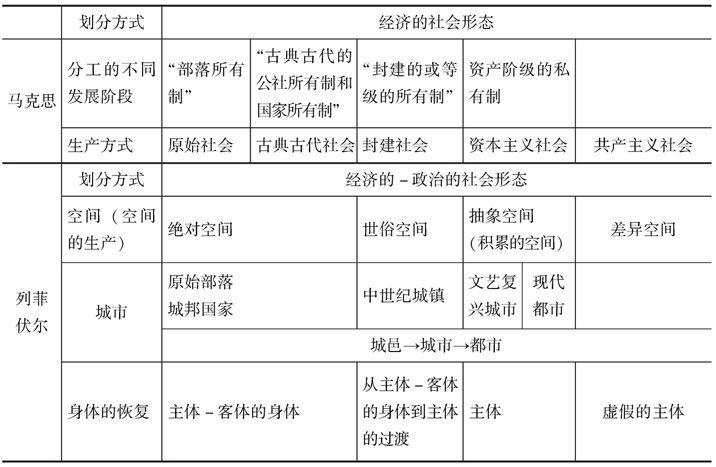
\includegraphics{images/00004.jpeg}
\end{figure}

再次,空间的三元分析是对马克思通过``资本---土地---劳动''理解社会的三元结构模式的恢复和发展。马克思指出:``把经济范畴按它们在历史上起决定作用的先后次序来排列是不行的,错误的。它们的次序倒是由它们在现代资产阶级社会中的相互关系决定的,这种关系同表现出来的它们的自然次序或者符合历史发展的次序恰好相反。问题不在于各种经济关系在不同社会形式的相继更替的序列中在历史上占有什么地位,更不在于它们在`观念上'(蒲鲁东)(在关于历史运动的一个模糊的表象中)的顺序。而在于它们在现代资产阶级社会内部的结构。''\protect\hypertarget{part0010_split_002.htmlux5cux23w53}{}{}\protect\hyperlink{part0010_split_002.htmlux5cux23m53}{\textsuperscript{{[}53{]}}}虽然马克思意识到要通过经济范畴之间的关系来理解资产阶级的生产方式,但在《资本论》中他却主要是以``资本---劳动''、``资产阶级---无产阶级''、``利润---工资''等二元模型来分析资本主义社会的矛盾和冲突。在列斐伏尔看来,二元分析固然能凸显和清晰地表达冲突,然而``土地''、``地租''、``地主''和``农业''这样的第三元要素消失了,并且,更重要的是,``带有冲突的(辩证的)特征的二元对立暗含着历史降低到经济的从属地位,无论是在现实还是在概念领域,也因而使具有历史继承性的、它们自身具有前资本主义特征的多样性的构成要素(城镇还有其他因素)被经济领域同化吸收。在这个图式的语境中,社会实践的空间是无法被觉察到的;时间扮演微不足道的角色;这个图式自身被放置在一个抽象的精神空间中。时间被简化为社会劳动的尺度。''\protect\hypertarget{part0010_split_002.htmlux5cux23w54}{}{}\protect\hyperlink{part0010_split_002.htmlux5cux23m54}{\textsuperscript{{[}54{]}}}在世界范围内,鉴于土地所有权、土地所有者、农业、地租等要素并没有消失,并且,地上、地面和地下甚至星际的空间资源日益重要,列斐伏尔提出,原本存在于马克思对资本主义社会分析中的三位一体图式需要被认识和澄清,分析资产阶级的生产方式需要分析土地、资本和劳动三个要素之间的关系。就土地这个要素来讲,在新资本主义社会里已经不仅仅指农业,还包括地上、地面和地下甚至星际的空间资源,这其中也应该包括受限于特定领土的民族国家。因此,政治活动和政治战略也是以往忽略的第三元要素的重要组成部分。列斐伏尔通过``空间的实践''、``空间的表象''和``具象的空间''的三位一体的分析图式就是要在历史性、社会性和空间性相统一的空间范畴中更好地解答新资本主义社会中资本、土地和劳动的关系,更好地分析国家和政治权力在资产阶级的生产方式中所起的重要作用,消除经济决定论的倾向,恢复存在于马克思思想中的通过多样性结构要素的相互关系分析社会现实的一元理论。

最后,从宏观范式到宏观和微观相结合的分析范式。马克思运用``二元分析''范式只是勾勒社会历史发展进程的粗线条,事实上,在社会历史的微观机制并未充分展现的时代条件下,马克思本人也更注重宏观的社会历史,而不是差异的、丰富的、多元的历史进程。衣俊卿指出:``马克思创立社会历史理论时所面对的社会现实是凭借宏大的经济力量而得以展开的,在这种语境中,马克思对人的自由和解放的理论设计更多地关注宏大的经济要素,更多地采用宏观解读和宏大叙事的研究范式,这实际上比较真实地反映了当时思想与对象的真实关系。''\protect\hypertarget{part0010_split_002.htmlux5cux23w55}{}{}\protect\hyperlink{part0010_split_002.htmlux5cux23m55}{\textsuperscript{{[}55{]}}}不过,\textbf{需要承认的是,马克思的社会历史理论中散落着丰富的微观理论资源,只不过马克思并未自觉地使用微观范式进行研究。比如,马克思对个人实践活动的强调,对个人与个人之间形成的丰富的社会关系的重视。}时至20世纪,随着工业社会的发展,传统占主导地位的宏观的政治和经济权力逐渐分化为``非中心化的、弥散的微观权力''。由此,人类的存在状态也日益表现为多样性、个别性和差异性。在这种条件下,列斐伏尔认为,在马克思那里占主导地位的宏观范式已不足以承担起解释社会历史的重任,而应引入微观范式,实现理论研究的宏观范式和微观范式的统一。他指出:``\,`宏观'和`微观'层面之间虽然存在着间距和鸿沟,但这并不意味着容许我们把其中的一个层面与另一个层面二分开来,更不允许我们`忽视'(scotomize)其中的某一个层面。''\protect\hypertarget{part0010_split_002.htmlux5cux23w56}{}{}\protect\hyperlink{part0010_split_002.htmlux5cux23m56}{\textsuperscript{{[}56{]}}}列斐伏尔所开启的日常生活批判研究以及空间批判理论研究正是宏观和微观范式相统一的典范。一方面,从对建筑、住宅、城市、地区、日常生活、身体等微观层面的研究切入到对空间战略、都市化、国家、全球化等宏观层面的研究,揭示了资本主义的基础性结构。另一方面,通过对资本主义整体结构和节奏的把握来分析资本主义的日常性、文化、权力、个人及其生活世界。总而言之,空间批判和节奏分析使社会历史的微观分析和宏观分析的结合有了现实的着力点或者基础。

\subsubsection{\texorpdfstring{(四)改变世界:从``暴力革命''到``空间革命''的转进}{(四)改变世界:从暴力革命到空间革命的转进}}\label{part0010_split_002.htmlux5cux23d042}

\textbf{马克思关于社会和历史的分析是以改变世界为旨趣的,革命的观点是他唯物主义的历史观的直接结果。马克思认为,革命是由生产力和与之相应的生产关系的变化决定的。他指出:``社会的物质生产力发展到一定阶段,便同它们一直在其中运动的现存生产关系或财产关系(这只是生产关系的法律用语)发生矛盾。于是这些关系便由生产力的发展形式变成生产力的桎梏。那时社会革命的时代就到来了。''}\protect\hypertarget{part0010_split_002.htmlux5cux23w57}{}{}\protect\hyperlink{part0010_split_002.htmlux5cux23m57}{\textsuperscript{{[}57{]}}}在谈到革命实践的必要条件时,马克思强调革命依赖于实现它的无产阶级,并且,成功的革命需要无产阶级是一个``自为''阶级。马克思曾乐观地设想,经济危机导致革命的发生,到那时,无产阶级将通过暴力革命开创人类历史的新纪元。然而,一次次经济危机的爆发并没有导致总体的社会革命的到来,资本主义在经历经济危机的凤凰涅槃之后浴火重生,如何改变世界成了二战后困扰马克思主义者的一个核心问题。

列斐伏尔从马克思的经典问题域出发来分析革命的根源、必要条件和可能性,当然是在引入了空间这个新概念的基础上。首先,列斐伏尔是从生产力和生产关系的辩证运动出发来理解总体的社会革命没有发生的原因的。一方面,抽象空间的生产实现了资本主义生产关系的再生产,作为生产方式的资本主义的存续使资本能够突破自身的界限,创造更大的生产力。另一方面,\textbf{从空间中物的生产发展到空间本身的生产不仅没有改变资本主义的生产方式,而且在更高的程度上巩固和加强了资本主义的生产关系。}正如马克思所言:``\textbf{无论哪一个社会形态,在它所能容纳的全部生产力发挥出来以前,是决不会灭亡的;而新的更高的生产关系,在它的物质存在条件在旧社会的胎胞里成熟以前,是决不会出现的。}''\protect\hypertarget{part0010_split_002.htmlux5cux23w58}{}{}\protect\hyperlink{part0010_split_002.htmlux5cux23m58}{\textsuperscript{{[}58{]}}}其次,列斐伏尔就工人阶级的革命性进行了分析。马克思把工人阶级理解为历史的主体的做法导致了在他之后的马克思主义中流行着工人阶级至上的思想趋势。\textbf{列斐伏尔认为,不仅理论上讲,作为一个阶级的工人阶级无法成为历史的主体,而且从新资本主义的社会实践来看,工人阶级也无法担负此重任。他指出,工人阶级并不天然地是革命的主体,工人阶级的革命性是情境性的。}伴随着空间成为资产阶级管理和控制社会的工具,无产阶级因空间的碎片化而分崩离析,变成了丧失批判意识的碎片化空间的``使用者'',如果没有先进的政治思想引导,它的革命性作用将难以发挥。最后,列斐伏尔认为,\textbf{改变世界需要不断革命,改变生活首先要改变空间。``改变生活''是列斐伏尔的``最高革命''理想。他把马克思改变世界的宏大目标转变成了彻底改变生活的微观实践。并且,在他看来,从微观践行到宏大目标的实现必然要经历一场持久的文化革命和政治经济革命。}他的空间分析中也透出此种隐忧。在新资本主义的空间生产中,自上而下的国家生产方式把日常生活规划为资本空间布展的基础,每个被规划的个体成了资本主义社会用以推动自身发展的力量。因而,要想撼动这种生产方式需要重塑被意识形态同化的个体。空间革命就是要使国家和政治权力对空间的生产和管理转变为每个个体对空间的占有和使用,也只有这样才能实现空间生产的全部潜力,产生新的空间,从而产生新的生活方式和新的世界。

综上所述,列斐伏尔的空间批判理论作为20世纪马克思主义理论发展进程中的一个富有影响力和创造力的理论形态,既与经典马克思主义和西方马克思主义有着扯不断的联系,同时又有所区别。在经典马克思主义那里,社会历史理论叙事的方式可以称作是``时间的政治'',时间范式压倒性地占据支配地位。时间解释的优先地位从根本上源于19世纪资本主义的经济活动更主要的是遵循着``用时间来消灭空间''的基本原则。尽管如此,马克思恩格斯的思想中存在着丰富的极富启发性的空间思想资源。马克思恩格斯思想中空间的``缺场''和``在场''共同促成了历史唯物主义的空间``转进''。本书从哲学范式、资本主义批判的逻辑起点、方法到理论旨归对列斐伏尔的空间分析所实现的历史唯物主义的空间``转进''进行了分析和阐释。列斐伏尔的空间批判理论在马克思的现代哲学范式内,以生产性的``社会空间''概念为中介,通过对社会历史发展的宏观把握和具体社会生活的微观分析,实现了对生活世界和个体的社会生存的深切关照。在此意义上,列斐伏尔的空间批判理论在资本主义社会新的时代语境中重新激活了马克思的生产理论,并在空间生产的辩证法中重构了革命主体的生产逻辑。我们不得不承认,与经典马克思主义相比,空间批判理论富有创造性地开启了马克思主义的当代性。然而,列斐伏尔的空间分析尽管强调和彰显了社会生活不可或缺的空间性,丰富和完善了历史唯物主义的空间化维度,在劳动、商品、生产力、生产关系、经济基础、上层建筑等经典范畴基础上发展了一系列新的概念,但究其根本还是自囿于马克思的``非异化---异化---非异化''(``差异空间---异化的(社会空间)---差异空间'')的图式中不能自拔。\textbf{尽管列斐伏尔把马克思寄托于无产阶级革命的理想变成更广泛的无产阶层改变空间和改变生活的试验性乌托邦,但是,从总体上来说,空间化的历史唯物主义本质上还是以时间为演进线索的社会历史解释模式。}但无论如何,列斐伏尔的空间批判理论对于丰富马克思主义的社会历史理论具有独特的价值,是西方马克思主义多样化的理论谱系中一道别样的风景。他的理论再一次提醒我们,马克思学说的生命力和革命性就在于,它坚持不懈地揭示人类历史发展中处于真实的、活生生的社会生活中的东西,是辩证地考察具体社会历史现实并随时代的演进而不断发展的批判理论。

\begin{center}\rule{0.5\linewidth}{\linethickness}\end{center}

\protect\hypertarget{part0010_split_002.htmlux5cux23m1}{}{}\protect\hyperlink{part0010_split_001.htmlux5cux23w1}{{[}1{]}}
Henri Lefebvre,\emph{Critique of Everyday
Life,Vol.I,Introduction},Translated by John Moore,Preface by Michel
Trebtish,London and New York:Verso,1991,p.76.

\protect\hypertarget{part0010_split_002.htmlux5cux23m2}{}{}\protect\hyperlink{part0010_split_001.htmlux5cux23w2}{{[}2{]}}
〔美〕爱德华·索杰:《第三空间》,陆扬等译,上海教育出版社,2005,第2页。

\protect\hypertarget{part0010_split_002.htmlux5cux23m3}{}{}\protect\hyperlink{part0010_split_001.htmlux5cux23w3}{{[}3{]}}
〔美〕爱德华·索杰:《第三空间》,陆扬等译,上海教育出版社,2005,第1页。

\protect\hypertarget{part0010_split_002.htmlux5cux23m4}{}{}\protect\hyperlink{part0010_split_001.htmlux5cux23w4}{{[}4{]}}
在哈维的《资本的限制》、《新帝国主义》等著作中均有对``空间修复''或者``时间---空间修复''理论的阐释。

\protect\hypertarget{part0010_split_002.htmlux5cux23m5}{}{}\protect\hyperlink{part0010_split_001.htmlux5cux23w5}{{[}5{]}}
〔英〕安东尼·吉登斯:《历史唯物主义的当代批判:权力、财产与国家》,郭忠华译,上海译文出版社,2010,第143页。

\protect\hypertarget{part0010_split_002.htmlux5cux23m6}{}{}\protect\hyperlink{part0010_split_001.htmlux5cux23w6}{{[}6{]}}
Neil Brenner,Stuart Elden.``Henri Lefebvre on
State,Space,Territory''. \emph{International Political
Sociology},2009(3):p.357.

\protect\hypertarget{part0010_split_002.htmlux5cux23m7}{}{}\protect\hyperlink{part0010_split_002.htmlux5cux23w7}{{[}7{]}}
〔英〕戴维·麦克莱伦:《马克思以后的马克思主义》,李智译,中国人民大学出版社,2008,第2页。

\protect\hypertarget{part0010_split_002.htmlux5cux23m8}{}{}\protect\hyperlink{part0010_split_002.htmlux5cux23w8}{{[}8{]}}
马克思、恩格斯:《神圣家族,或对批判的批判所做的批判》,《马克思恩格斯文集》(第1卷),人民出版社,2009,第295页。

\protect\hypertarget{part0010_split_002.htmlux5cux23m9}{}{}\protect\hyperlink{part0010_split_002.htmlux5cux23w9}{{[}9{]}}
马克思:《1844年经济学哲学手稿》,人民出版社,2000,第92页。

\protect\hypertarget{part0010_split_002.htmlux5cux23m10}{}{}\protect\hyperlink{part0010_split_002.htmlux5cux23w10}{{[}10{]}}
马克思:《1844年经济学哲学手稿》,《马克思恩格斯文集》(第1卷),人民出版社,2009,第161页。

\protect\hypertarget{part0010_split_002.htmlux5cux23m11}{}{}\protect\hyperlink{part0010_split_002.htmlux5cux23w11}{{[}11{]}}
马克思:《1844年经济学哲学手稿》,《马克思恩格斯文集》(第1卷),人民出版社,2009,第210页。

\protect\hypertarget{part0010_split_002.htmlux5cux23m12}{}{}\protect\hyperlink{part0010_split_002.htmlux5cux23w12}{{[}12{]}}
马克思:《1844年经济学哲学手稿》,《马克思恩格斯文集》(第1卷),人民出版社,2009,第233页。

\protect\hypertarget{part0010_split_002.htmlux5cux23m13}{}{}\protect\hyperlink{part0010_split_002.htmlux5cux23w13}{{[}13{]}}
恩格斯:《论住宅问题》,《马克思恩格斯文集》(第3卷),人民出版社,2009,第307页。

\protect\hypertarget{part0010_split_002.htmlux5cux23m14}{}{}\protect\hyperlink{part0010_split_002.htmlux5cux23w14}{{[}14{]}}
恩格斯:《论住宅问题》,《马克思恩格斯文集》(第3卷),人民出版社,2009,第307页。

\protect\hypertarget{part0010_split_002.htmlux5cux23m15}{}{}\protect\hyperlink{part0010_split_002.htmlux5cux23w15}{{[}15{]}}
马克思、恩格斯:《德意志意识形态》,《马克思恩格斯文集》(第1卷),人民出版社,2009,第556页。

\protect\hypertarget{part0010_split_002.htmlux5cux23m16}{}{}\protect\hyperlink{part0010_split_002.htmlux5cux23w16}{{[}16{]}}
恩格斯:《论权威》,《马克思恩格斯文集》(第3卷),人民出版社,2009,第336页。

\protect\hypertarget{part0010_split_002.htmlux5cux23m17}{}{}\protect\hyperlink{part0010_split_002.htmlux5cux23w17}{{[}17{]}}
马克思:《资本论》(第1卷),《马克思恩格斯文集》(第5卷),人民出版社,2009,第491页。

\protect\hypertarget{part0010_split_002.htmlux5cux23m18}{}{}\protect\hyperlink{part0010_split_002.htmlux5cux23w18}{{[}18{]}}
马克思:《资本论》(第2卷),《马克思恩格斯文集》(第6卷),人民出版社,2009,第278页。

\protect\hypertarget{part0010_split_002.htmlux5cux23m19}{}{}\protect\hyperlink{part0010_split_002.htmlux5cux23w19}{{[}19{]}}
马克思:《资本论》(第2卷),《马克思恩格斯文集》(第6卷),人民出版社,2009,第279页。

\protect\hypertarget{part0010_split_002.htmlux5cux23m20}{}{}\protect\hyperlink{part0010_split_002.htmlux5cux23w20}{{[}20{]}}
马克思、恩格斯:《共产党宣言》,《马克思恩格斯文集》(第2卷),人民出版社,2009,第35页。

\protect\hypertarget{part0010_split_002.htmlux5cux23m21}{}{}\protect\hyperlink{part0010_split_002.htmlux5cux23w21}{{[}21{]}}
马克思、恩格斯:《共产党宣言》,《马克思恩格斯文集》(第2卷),人民出版社,2009,第37页。

\protect\hypertarget{part0010_split_002.htmlux5cux23m22}{}{}\protect\hyperlink{part0010_split_002.htmlux5cux23w22}{{[}22{]}}
〔英〕戴维·哈维:《马克思的空间转移理论------〈共产党宣言〉的地理学》,郇建立编译,《马克思主义与现实》2005年第4期。

\protect\hypertarget{part0010_split_002.htmlux5cux23m23}{}{}\protect\hyperlink{part0010_split_002.htmlux5cux23w23}{{[}23{]}}
马克思、恩格斯:《共产党宣言》,《马克思恩格斯文集》(第2卷),人民出版社,2009,第37页。

\protect\hypertarget{part0010_split_002.htmlux5cux23m24}{}{}\protect\hyperlink{part0010_split_002.htmlux5cux23w24}{{[}24{]}}
恩格斯:《英国工人阶级状况》,《马克思恩格斯文集》(第1卷),人民出版社,2009,第402页。

\protect\hypertarget{part0010_split_002.htmlux5cux23m25}{}{}\protect\hyperlink{part0010_split_002.htmlux5cux23w25}{{[}25{]}}
恩格斯:《英国工人阶级状况》,《马克思恩格斯文集》(第1卷),人民出版社,2009,第402页。

\protect\hypertarget{part0010_split_002.htmlux5cux23m26}{}{}\protect\hyperlink{part0010_split_002.htmlux5cux23w26}{{[}26{]}}
马克思:《不列颠在印度的统治》,《马克思恩格斯文集》(第2卷),人民出版社,2009,第683页。

\protect\hypertarget{part0010_split_002.htmlux5cux23m27}{}{}\protect\hyperlink{part0010_split_002.htmlux5cux23w27}{{[}27{]}}
马克思:《路易波拿巴的雾月十八日》,《马克思恩格斯文集》(第2卷),人民出版社,2009,第566页。

\protect\hypertarget{part0010_split_002.htmlux5cux23m28}{}{}\protect\hyperlink{part0010_split_002.htmlux5cux23w28}{{[}28{]}}
恩格斯:《德国的革命和反革命》,《马克思恩格斯文集》(第2卷),人民出版社,2009,第357页。

\protect\hypertarget{part0010_split_002.htmlux5cux23m29}{}{}\protect\hyperlink{part0010_split_002.htmlux5cux23w29}{{[}29{]}}
马克思、恩格斯:《德意志意识形态》,《马克思恩格斯文集》(第1卷),人民出版社,2009,第539页。

\protect\hypertarget{part0010_split_002.htmlux5cux23m30}{}{}\protect\hyperlink{part0010_split_002.htmlux5cux23w30}{{[}30{]}}
恩格斯:《家庭、私有制和国家的起源》,《马克思恩格斯文集》(第4卷),人民出版社,2009,第178页。

\protect\hypertarget{part0010_split_002.htmlux5cux23m31}{}{}\protect\hyperlink{part0010_split_002.htmlux5cux23w31}{{[}31{]}}
马克思:《工资、价格和利润》,《马克思恩格斯文集》(第3卷),人民出版社,2009,第70页。

\protect\hypertarget{part0010_split_002.htmlux5cux23m32}{}{}\protect\hyperlink{part0010_split_002.htmlux5cux23w32}{{[}32{]}}
马克思、恩格斯:《共产党宣言》,《马克思恩格斯文集》(第2卷),人民出版社,2009,第36页。

\protect\hypertarget{part0010_split_002.htmlux5cux23m33}{}{}\protect\hyperlink{part0010_split_002.htmlux5cux23w33}{{[}33{]}}
马克思、恩格斯:《德意志意识形态》,《马克思恩格斯文集》(第1卷),人民出版社,2009,第539页。

\protect\hypertarget{part0010_split_002.htmlux5cux23m34}{}{}\protect\hyperlink{part0010_split_002.htmlux5cux23w34}{{[}34{]}}
马克思、恩格斯:《德意志意识形态》,《马克思恩格斯文集》(第1卷),人民出版社,2009,第537页。

\protect\hypertarget{part0010_split_002.htmlux5cux23m35}{}{}\protect\hyperlink{part0010_split_002.htmlux5cux23w35}{{[}35{]}}
张一兵主编《资本主义理解史》第一卷,江苏人民出版社,2009,第471页。

\protect\hypertarget{part0010_split_002.htmlux5cux23m36}{}{}\protect\hyperlink{part0010_split_002.htmlux5cux23w36}{{[}36{]}}
马克思:《关于费尔巴哈的提纲》,《马克思恩格斯选集》(第1卷),人民出版社,1995,第56页。

\protect\hypertarget{part0010_split_002.htmlux5cux23m37}{}{}\protect\hyperlink{part0010_split_002.htmlux5cux23w37}{{[}37{]}}
马克思:《〈政治经济学批判〉序言》,《马克思恩格斯选集》(第2卷),人民出版社,1995,第32页。

\protect\hypertarget{part0010_split_002.htmlux5cux23m38}{}{}\protect\hyperlink{part0010_split_002.htmlux5cux23w38}{{[}38{]}}
Henri Lefebvre,\emph{The Survival of Capitalism}. Translated by Frank
Bryant,London:Allison \& Busby,1976,p.17.

\protect\hypertarget{part0010_split_002.htmlux5cux23m39}{}{}\protect\hyperlink{part0010_split_002.htmlux5cux23w39}{{[}39{]}}
Henri Lefebvre,\emph{The Production of Space}. Translated by Donald
Nicholson-Smith,Basil Blackwell Ltd,1991,p.129.

\protect\hypertarget{part0010_split_002.htmlux5cux23m40}{}{}\protect\hyperlink{part0010_split_002.htmlux5cux23w40}{{[}40{]}}
吉尔·德勒兹:《尼采与哲学》,周颖、刘玉宇译,社会科学文献出版社,2001,第59页。

\protect\hypertarget{part0010_split_002.htmlux5cux23m41}{}{}\protect\hyperlink{part0010_split_002.htmlux5cux23w41}{{[}41{]}}
Henri Lefebvre,\emph{The Production of Space}. Translated by Donald
Nicholson-Smith,Basil Blackwell Ltd,1991,p.405.

\protect\hypertarget{part0010_split_002.htmlux5cux23m42}{}{}\protect\hyperlink{part0010_split_002.htmlux5cux23w42}{{[}42{]}}
马克思:《资本论》第一卷1872年第二版跋,《马克思恩格斯选集》(第2卷),人民出版社,1995,第106页。

\protect\hypertarget{part0010_split_002.htmlux5cux23m43}{}{}\protect\hyperlink{part0010_split_002.htmlux5cux23w43}{{[}43{]}}
马克思:《资本论》第一卷,《马克思恩格斯选集》(第2卷),人民出版社,1995,第114页。

\protect\hypertarget{part0010_split_002.htmlux5cux23m44}{}{}\protect\hyperlink{part0010_split_002.htmlux5cux23w44}{{[}44{]}}
Henri Lefebvre,\emph{The Production of Space}. Translated by Donald
Nicholson-Smith,Basil Blackwell Ltd,1991,p.337.

\protect\hypertarget{part0010_split_002.htmlux5cux23m45}{}{}\protect\hyperlink{part0010_split_002.htmlux5cux23w45}{{[}45{]}}
Henri Lefebvre,\emph{The Production of Space}. Translated by Donald
Nicholson-Smith,Basil Blackwell Ltd,1991,p.337.

\protect\hypertarget{part0010_split_002.htmlux5cux23m46}{}{}\protect\hyperlink{part0010_split_002.htmlux5cux23w46}{{[}46{]}}
Henri Lefebvre,``Space and Mode of Production,''
\emph{State,Space,World:Selected Essays}. Minneapolis ·
London:University of Minnesota Press,2009,pp.213-214.

\protect\hypertarget{part0010_split_002.htmlux5cux23m47}{}{}\protect\hyperlink{part0010_split_002.htmlux5cux23w47}{{[}47{]}}
马克思:《〈政治经济学批判〉导言》,《马克思恩格斯选集》(第2卷),人民出版社,1995,第23页。

\protect\hypertarget{part0010_split_002.htmlux5cux23m48}{}{}\protect\hyperlink{part0010_split_002.htmlux5cux23w48}{{[}48{]}}
马克思:《〈政治经济学批判〉导言》,《马克思恩格斯选集》(第2卷),人民出版社,1995,第23页。

\protect\hypertarget{part0010_split_002.htmlux5cux23m49}{}{}\protect\hyperlink{part0010_split_002.htmlux5cux23w49}{{[}49{]}}
Henri Lefebvre,\emph{The Production of Space}. Translated by Donald
Nicholson-Smith,Basil Blackwell Ltd,1991,p.64.

\protect\hypertarget{part0010_split_002.htmlux5cux23m50}{}{}\protect\hyperlink{part0010_split_002.htmlux5cux23w50}{{[}50{]}}
马克思:《〈政治经济学批判〉导言》,《马克思恩格斯选集》(第2卷),人民出版社,1995,第24页。

\protect\hypertarget{part0010_split_002.htmlux5cux23m51}{}{}\protect\hyperlink{part0010_split_002.htmlux5cux23w51}{{[}51{]}}
Henri Lefebvre,\emph{The Production of Space}. Translated by Donald
Nicholson-Smith,Basil Blackwell Ltd,1991,p.65.

\protect\hypertarget{part0010_split_002.htmlux5cux23m52}{}{}\protect\hyperlink{part0010_split_002.htmlux5cux23w52}{{[}52{]}}
马克思:《〈政治经济学批判〉导言》,《马克思恩格斯选集》(第2卷),人民出版社,1995,第24页。

\protect\hypertarget{part0010_split_002.htmlux5cux23m53}{}{}\protect\hyperlink{part0010_split_002.htmlux5cux23w53}{{[}53{]}}
马克思:《〈政治经济学批判〉导言》,《马克思恩格斯选集》(第2卷),人民出版社,1995,第25页。

\protect\hypertarget{part0010_split_002.htmlux5cux23m54}{}{}\protect\hyperlink{part0010_split_002.htmlux5cux23w54}{{[}54{]}}
Henri Lefebvre,\emph{The Production of Space}. Translated by Donald
Nicholson-Smith,Basil Blackwell Ltd,1991,p.324.

\protect\hypertarget{part0010_split_002.htmlux5cux23m55}{}{}\protect\hyperlink{part0010_split_002.htmlux5cux23w55}{{[}55{]}}
衣俊卿:《历史唯物主义与当代社会历史现实》,《中国社会科学》2011年第3期。

\protect\hypertarget{part0010_split_002.htmlux5cux23m56}{}{}\protect\hyperlink{part0010_split_002.htmlux5cux23w56}{{[}56{]}}
衣俊卿编《社会历史理论的微观视域》,黑龙江大学出版社、中央编译出版社,2011,第550页。

\protect\hypertarget{part0010_split_002.htmlux5cux23m57}{}{}\protect\hyperlink{part0010_split_002.htmlux5cux23w57}{{[}57{]}}
马克思:《〈政治经济学批判〉序言》,《马克思恩格斯选集》(第2卷),人民出版社,1995,第32页。

\protect\hypertarget{part0010_split_002.htmlux5cux23m58}{}{}\protect\hyperlink{part0010_split_002.htmlux5cux23w58}{{[}58{]}}
马克思:《〈政治经济学批判〉序言》,《马克思恩格斯选集》(第2卷),人民出版社,1995,第33页。

\protect\hypertarget{part0011.html}{}{}

\hypertarget{part0011.htmlux5cux23a011}{\chapter{结语}\label{part0011.htmlux5cux23a011}}

在列斐伏尔的空间批判理论中,始终有一个基本问题贯穿始终。那就是,\textbf{新资本主义社会关系的存在方式究竟是什么?}

社会科学自信研究社会关系便可把握社会的存在和发展。问题是,当社会关系尚未实现时,它定居在何处?它以何种方式存在?它以何种状态发生作用?显然,社会科学并没有给出答案,似乎它更重视社会关系的形式、结构和功能,而非社会关系的存在方式。这也就意味着,社会科学常常把应该加以研究的前提当作不证自明的前提。当人们不知社会关系如何存在时,很难想象运用社会关系能解释社会整体的存在状态。不过,社会科学都肯定了一个基本事实:社会关系不能脱离开它的物质基础。随之而来的问题是,社会关系的物质基础如何发挥它的功能?在列斐伏尔看来,以往的思想家并没有把这个问题作为问题认真对待,包括马克思。马克思肯定了社会关系有其物质基础,并把物质基础看作解释和支撑社会关系的根本。然而,马克思清楚地讲道,物作为商品就不再是物了。因为,社会生活中的物都体现着一定的社会关系,正如商品体现着资本主义的交换关系一样。一旦物(商品)分解进特定的社会关系,那么物也就不存在了,社会关系便恢复为它的抽象性。列斐伏尔认为,马克思只是表面地解决了这个问题。

正因为如此,列斐伏尔引入了社会空间概念,以此来完成马克思当年未完成而且由于时代条件所限不能完成的任务。可以说,列斐伏尔空间批判的独特理论贡献就在于两大发现:一是将空间的生产视为资本主义存续和发展的社会历史过程,打破了以历史为中心的马克思主义文化传统;二是揭示了内蕴于空间生产这一资本主义历史进程的政治和意识形态,阐明了空间的政治性。空间是新资本主义国家和政治权力的工具,空间的生产是新资本主义的政治策略。列斐伏尔在汲取黑格尔、马克思和尼采思想的基础上创造性地提出了三元辩证法,以此来展开对空间的历史性分析和社会性以及资本主义的空间逻辑的分析。\textbf{他的结论可概括为如下八个方面}。

\textbf{第一,空间是社会的。按照空间的存在样态,空间可分为自然空间和社会空间。但是,列斐伏尔认为,真正现实的空间只能是社会的,现实的空间必然和一定的人类实践活动方式或生产方式相关联。}基于这种见解,他按照空间与生产方式的关系将空间的历史形态依次划分为与亚细亚生产方式相适应的自然空间、与奴隶制生产方式相适应的绝对空间、与封建制生产方式相适应的世俗空间以及与资本主义生产方式相适应的抽象空间。每一种空间都标示着特定生产方式和生产关系的印记,在一定意义上,前者也是后者的存在方式。这一见解是空间批判理论展开的基本前提。

\textbf{第二,与19世纪资本主义生产方式凸显时间的优先性相对立,20世纪资本主义生产方式凸显出空间的优先性,空间消灭了时间。}列斐伏尔认为,马克思之所以谈及空间问题而未充分展开,根本而言,在于19世纪资本主义生产方式遵循的基本原则是``用时间消灭空间''。而20世纪资本主义生产方式已然进行了调整,空间在社会中获得越来越重要的角色。\textbf{概括来说,资本主义由原来的``空间中物的生产''转变为``空间的生产''。}空间不再作为自然独创性的作品,而成为可以批量生产和复制的产品和商品。世界市场、劳动分工、计算机科学空间、战略愿景空间、建筑风格、都市主义等都充分体现着空间生产的痕迹。

\textbf{第三,20世纪资本主义生产的空间是抽象空间。}列斐伏尔认为,在资本主义理性化原则的支配下,空间越来越成为抽象的。这种抽象性集中表现在\textbf{空间的同质性、碎片化和等级化。同质化意味着空间被剥去了物质材料基础,失去了它的质的独特性,而成为可以被完全量化而进行交换的产品。碎片化意味着整体的空间按照资本主义的战略需要被分割成各种各样具有经济功能的空间。等级化意味着整体的空间按照资本主义的政治权力体系被塑造成一定社会等级的空间。}

\textbf{第四,空间的生产是资本主义战略实践的产物。空间的生产是资本主义秩序中多种要素综合作用的结果,包括资本、市场、人口、科技、意识形态等。但其中最主要的一个要素是国家和政治权力。}现代国家战略性地组织起一种可量化的理性,这不仅使得经济增长成为可能,并使国家从这种增长中获得占领整个星球的力量。\textbf{在国家生产方式的支配下,空间成为政治工具,空间的生产成为政治权力渗透和扩张的有效途径。}

\textbf{第五,``空间的生产''的本质是资本主义生产关系的再生产。}列斐伏尔认为,20世纪资本主义之所以能够幸存的秘密在于生产关系的再生产。空间的生产绝非偶然出现或无意识的产物,而是资本主义的发展战略。这种战略实践的结果是,空间不再是生产的背景或物的寓所,而成为生产的根本性要素,特别是再生产的一部分。因此,空间的生产也不再是纯粹的物的生产,而从根本上是生产关系的再生产。\textbf{资本主义通过``开发''和``占用''空间,为生产关系的存在以及生产关系的再生产提供场所,这个过程同时也是生产关系再生产的过程。}

\textbf{第六,``空间的生产''进一步巩固了资本主义对社会日常生活的微观操控。}通过生产的空间网络,资本和政治权力的触角延伸至社会的各个层面和各个领域,形成了一种普遍性的操控机制。这种操控不仅表现为人们总是处于由各种权力关系交织的社会空间中,而且还表现为抽象空间``拜物教''的形成。结果便是,日常生活及其生活于其中的人的异化状态被加重了,同时,这种异化状态配合着空间的生产的节奏再生产着异化状态。这是列斐伏尔空间批判理论的要旨所在。

\textbf{第七,空间批判理论致力于异化的扬弃。资本主义的空间实践一方面加重了人的异化,另一方面生产出诸多矛盾,比如中心和边缘、都市和乡村、同质和差异等。}当这些矛盾发展到临界点时,便指向了差异冲破同质和异化扬弃的可能性。那些处于边缘的人群,新条件下的工人阶级、时间和空间中的差异、生命意识、自我管理等都有可能成为革命的要素。这是空间批判理论的目的所在。

\textbf{第八,资本主义对日常生活的操控是对时间和空间总体规划的结果。在新资本主义社会中,和空间一样,时间被规划、组织和管理。总体而言,资本主义用抽象的、线性的、重复的时间置换了具体的、生命的、感性的时间,时间也日益呈现同质化、碎片化和等级化的特征。}通过对时间和空间的整体规划,资本主义强化了对日常生活的控制。不过,如同空间中的差异力量一样强大,时间中的差异因素有可能成为革命的要素。

总之,作为日常生活批判理论进一步深化的空间批判理论,深刻而独特地揭示了现代资本主义的文化危机和运行机制,不仅实现了社会历史理论研究从宏观范式到微观范式、从经济范式到文化范式的转换。而且,列斐伏尔以对空间、国家和日常生活的三重批判重构了关于现代世界的``马克思主义的''问题系,使导源于马克思的各种概念和范畴重新获得了思想的整体性,对马克思的社会历史理论来说是一种丰富和发展。

更为重要的是,空间批判理论开启了马克思主义社会历史理论研究的一个新视域。在全球化语境和新的思想空间中,列斐伏尔的空间批判思想一直在以或者光鲜或者隐晦的方式,被人们反复解读。无疑,空间具有重要作用,这似乎是一个不争的事实。生活常识通常会告知我们,如果我们与另一些事物打交道,自身和它们就必须处于适当的位置。如果没有空间,很难想象物的存在和变化。如果没有一种合理的空间,很难想象人的健康发展。正如待在一个暗无天日的狭窄空间中,人的精神状态会紊乱。然而,令人奇怪的是,在20世纪以前,众多学科似乎更喜欢研究时间,空间或多或少被忽视甚至遗忘。近代西方哲学按照数学或物理学的方式将空间理解为空荡荡的``容器''。即使在马克思那里,这种问题虽因唯物辩证法的引入而得以缓解,但空间仍未被充分关注。直至列斐伏尔空间批判理论的出现,空间才被拉回到人们的视野中。当列斐伏尔揭示出空间概念丰富的社会内涵时,人们才恍然大悟,原来空间早已不再仅仅是想象中的和某物直接同一的自然空间,而成为某种被社会关系规定的社会空间。可以说,空间批判理论革命性地打破了社会历史理论研究中时间范式的支配性地位,把空间引入了社会历史领域。此举在人类思想发展历程中不能不说是一次革命。这也就不难理解为什么列斐伏尔去世之后,他的思想持续升温,或者说经历了一次令人惊讶的复兴。

当然,列斐伏尔的范畴、方法和分析为整体上理解资本主义有机体这个艰巨的任务只提供了一种视角。这里我们已经努力挖掘了他著作中的深刻洞见,这些洞见可以被运用来达到这一目的,但是资本主义社会中很多经济的、文化的和政治的因素仍然需要进一步挖掘。

从历史的观点来看,列斐伏尔的空间批判理论中仍存在着一些常见的疏忽:比如,他认为马克思只是把空间看作``生产场所的总和'',这种见解在一定程度上是有失偏颇的。从概念的角度来看,对一些关键性问题,列斐伏尔很少直接面对,而更多的是采取``迂回战术''。比如,生产关系和生产方式这些基本概念,他几乎没有集中系统的论述。\textbf{从政治的观点来看,列斐伏尔的空间批判理论在很大程度上主要是对他生活和工作的战后法国全盛的福特主义时期进行综合诊断。}因此,为了使空间批判理论与处于时刻变化和调整中的资本主义相适应,列斐伏尔的概念和分析肯定是不充足的,必然会受到挑战,并需要立足新的社会现实重新阐释。如果我们充分肯定空间批判理论,那么最好是把它看作为进一步思考和探索提供了刺激,提供了应对多种挑战的方法。正如马克思的学说在列斐伏尔那里接受了辩证的批判一样,空间批判理论注定遭此命运。或许这也是列斐伏尔希望看到的。

至此,我们也可以对列斐伏尔的整个学术生涯和思想演进的大体脉络作总结。他的理论出发点是马克思的异化理论和总体的人,他以此为基点而致力于揭示资本主义条件下的现代性危机。因此,可以把他的理论从总体上概括为一种现代性批判,而日常生活批判、空间批判和节奏分析都是这一独特的现代性批判的有机组成部分,它们不断深化列斐伏尔的现代性批判思想。具体说来:第一,在列斐伏尔看来,当今资本主义已经进入一个全面异化的状态,而日常生活的异化深刻地展示了当代社会异化的深度和广度:原本作为社会生活和社会运行的隐形结构、作为自在的意义结构的日常生活异化为资本主义生产关系和社会关系的基础,在微观层面支撑了资本主义的统治。第二,空间批判深刻揭示了日常生活异化的机制。应当说,日常生活的异化同马克思所描述的典型的劳动异化有很大的不同,它不仅与私有制和分工密切相关,而且与资本主义的空间生产直接相关,正是作为资本主义生产关系和社会关系再生产的空间生产及其都市化战略导致了日常生活的全面被规划和普遍异化,从而以其同质性、碎片化和等级化的特征成为资本主义统治的深层的和微观的基础。第三,\textbf{节奏分析又进一步深化了日常生活批判和空间批判的现代性批判主题。空间生产对现代社会生活的普遍操控和对日常生活的全面规划,实际上是借助多种单调的、线性重复的社会生活节奏及其各种微观权力编织而成的社会空间,即都市化战略而实现的,这种单调的线性的社会节奏压倒周期循环性的自然节奏成为现代日常生活的主要节奏,并且内化到现代人的生存结构之中,这又从一个侧面显示了日常生活异化的深度。}综上所述,日常生活批判、空间批判和节奏分析相互联系地构成了列斐伏尔现代性批判的有机组成部分,而超越现代性危机和资本的逻辑也需要在日常生活、空间生产和节奏分析中寻找潜能和资源。

站在21世纪的门槛里,我们不难感受到,与列斐伏尔在20世纪所作的探索一样,21世纪的思想家们仍致力于从微观层面寻求能指导具体社会历史实践的批判理论与宏观历史解释模式相连接的方式,只要资本主义作为一种生产方式还继续存在,只要人类还在寻找真正自由解放的路上。异彩纷呈的理论盛宴总让人应接不暇,伟大的思想总在相互交锋和相互渗透中更具生命力和革命性。之所以它们的具体进路不同,是因为对人类所面临的重大理论问题和现实问题及其变化的认识和分析各有千秋,而马克思主义的危机和复兴即源于此。借用安东尼奥·拉布里奥拉(Antonio Labriola)的话来说便是:``使得马克思主义的不完美如此明显的真正的新世界是什么?这就是困难之所在。''\protect\hypertarget{part0011.htmlux5cux23w1}{}{}\protect\hyperlink{part0011.htmlux5cux23m1}{\textsuperscript{{[}1{]}}}``真正的新世界是什么''就如同一块巨石,使每一个想``改变世界''的人如西西弗斯般经受磨难,但同样,也如西西弗斯般怀有激情并勇往直前。

\begin{center}\rule{0.5\linewidth}{\linethickness}\end{center}

\protect\hypertarget{part0011.htmlux5cux23m1}{}{}\protect\hyperlink{part0011.htmlux5cux23w1}{{[}1{]}}
转引自〔法〕雅克·比岱、〔法〕厄斯塔什·库维拉基斯主编《当代马克思辞典》,许国艳等译,社会科学文献出版社,2011,第82页。

\protect\hypertarget{part0012.html}{}{}

\hypertarget{part0012.htmlux5cux23a012}{\chapter{参考文献}\label{part0012.htmlux5cux23a012}}

\textbf{一 外文文献}

\textbf{1.列斐伏尔的著作}

Henri Lefebvre,\emph{Dialectical Materialism}. London:Jonathan Cape
Ltd,1968.

Henri Lefebvre,\emph{The Sociology of Marx}. New York:Columbia
University Press,1969.

Henri Lefebvre,\emph{Introduction to Modernity}. London and New
York:Verso,1995.

Henri Lefebvre,\emph{Everyday Life in the Modern World}. New
Brunswick:Transaction Publishers,1994.

Henri Lefebvre,\emph{Writings on Cities}. Oxford UK \& Cambridge
USA:Blackwell Publishers Ltd,1996.

Henri Lefebvre,\emph{The Urban Revolution}. London:University of
Minnesota Press,2003.

Henri Lefebvre,\emph{The Survival of Capitalism}. London:Allison \&
Busby,1976.

Henri Lefebvre,\emph{The Production of Space}. Oxford UK \& Cambridge
USA:Blackwell Publishers Ltd,1991.

Henri Lefebvre,\emph{Rhythmanalysis:Space,Time and Everyday Life}.
London and New York:Continuum,2004.

Henri Lefebvre,\emph{Critique of Everyday
Life,Vol.I:Introduction}.London and New York:Verso,1991.

Henri Lefebvre,\emph{Critique of Everyday Life,Vol.II:Foundation of a
Sociology of Everyday Life}. London and New York:Verso,2002.

Henri Lefebvre,\emph{Critique of Everyday Life,Vol.III,From Modernity
to Modernism(Towards a Metaphilosophy of Daily Life)}.London and New
York:Verso,2003.

Henri Lefebvre,\emph{Key Writings}. Edited by Stuart Elden,Elizabeth
Lebas and Eleonore Kofman,New York and London:Continuum,2003.

Henri Lefebvre,\emph{State,Space,World:Selected Essays}. Minneapolis
· London:University of Minnesota Press,2009.

Henri Lefebvre,\emph{Critique de la vie quotidienne,I:Introduction}.
Paris:Grasset,1947.

Henri Lefebvre,\emph{Critique de la vie quotidienne,II:Foudements
d'une sociologie de la quotidiennete}. Paris:L'Arche,1961-1987.

Henri Lefebvre,\emph{Critique de la vie quotidienne,III:De la
modernite au modernisme(pour une metaphilosophie du
quotidien)}.Paris:L'Arche,1981-1987.

\textbf{2.研究列斐伏尔的著作和论文}

Edward W.Soja,\emph{Postmodern Geographies,The Reassertion of Space in
Critical Social Theory}. London:Verso,1989.

Edward W.Soja,\emph{Third Space:Journey to Los Angeles and Other
Real-and-Imagined Places}. Cambridge:Blackwell Publisher Inc.,1996.

Rob Shields,\emph{Lefebvre,Love and Struggle:Spatial Dialectics}.
London and New York:Routledge,1999.

Stuart Elden,\emph{Understanding Henri Lefebvre}. London and New
York:Continuum,2004.

Christian Stadt Schmid,\emph{Raum und Gesellschaft:Henri Lefebvre und
die Theorie der Produktion des Raumes}. Stuttgart:Steiner,2005.

Andy Merrifield,\emph{Henri Lefebvre:A Critical Introduction}. New
York and London:Routledge,Taylor \& Francis Group,2006.

Edited by Kanishka Goonewardena,Stefan Kipfer,Richard
Milgrom,Christian Schmid,\emph{Space,Difference,Everyday
Life:Reading Henri Lefebvre}. New York and London:Routledge,2008.

Laurence Costes,\emph{Henri Lefebvre:le droit à la ville:vers la
sociologie de l'urbain}. Paris:Ellipses,2009.

Chris Butler,\emph{Henri Lefebvre:Spatial Politics,Everyday Life and
the Right to the City}. London:Routledge-Cavendish,2010.

Tim Edensor,\emph{Geographies of Rhythm:Nature,Place,Mobilities and
Bodies}. Farnham,Surrey,England;Burlington,VT:Ashgate,2010.

Reme Hess,\emph{Henri Lefebvre et} 1'\emph{aventure du siecle}.
Paris:A.M. Métailié,1988.

Mark Purcell,``Excavating Lefebvre:The Right to the City and Its Urban
Politics of the Inhabitant''.\emph{GeoJournal},2002,Volume 58,Numbers
2-3,pp.99-108.

Harvey Molotch,``The Space of Lefebvre''.\emph{Theory and
Society},1993,Volume 22,Number 6,pp.887-895.

\textbf{3.其他相关文献}

Barbara Adam,\emph{Timewatch:The Social Analysis of Time}.
Cambridge:Polity Press,1995.

Perry Anderson,\emph{The Origins of Postmodermity}. London and New
York:Verso,1998.

John Ardagh,\emph{The New France:A Society in Transition}
1945-1977.Harmondsworth:Penguin,1977.

Jean Baudrillard,\emph{The Consumer Society}. London,1998.

Manuel Castells,\emph{The Urban Questions.A Marxism Approach}.
Cambridge:MIT Press,1977.

B.Frankel,\emph{The Post-industrial Utopians}. Oxford Blackwell,1987.

David Harvey,\emph{The Limits to Capital}. Oxford:Blackwell,1982.

David Harvey,\emph{The Condition of Postmodernity}.
Oxford:Blackwell,1989.

M.Gottdiener,\emph{Social Production of Urban Space}.
Austin:University of Teaxas,1985.

P.Hall,\emph{Cities of Tomorrow}. Oxford:Blackwell Publishers,1988.

R.Jacoby,\emph{Dialectic of Defeat:Contours of Western Marxism}.
Cambridge:Cambridge University Press,1981.

J.Kunstler,\emph{Home from Nowhere:Remaking Our Everyday World for
the} 21\emph{st Century}. New York:Simon \& Schuster,1996.

Jay Martin,\emph{Marxism and Totality,From Lukacs to Habermas}.
Oakland:University of California Press,1984.

Steven Best and Douglas Kellner,\emph{Postmodern Turn}. New York:The
Guilford Press,1997.

Michel de Certeau,\emph{The Practice of Everyday Life}.
Berkeley:University of California Press,1984.

\textbf{二 中文文献}

\textbf{1.列斐伏尔的著作及相关研究文献}

〔法〕亨利·列菲弗尔:《论国家》,李青宜等译,重庆出版社,1988。

〔法〕亨利·列菲弗:《空间与政治》(第二版),李春译,上海人民出版社,2008。

〔法〕勒费弗尔:《马克思主义的分化》,张伯霖译,《哲学译丛》1980年第5期。

〔法〕列费弗尔:《研究日常生活的哲学家------列费弗尔答法国〈世界报〉记者问》,《国外社会科学动态》1983年第9期。

〔法〕列费弗尔:《马克思主义在法国的状况》,《国外社会科学动态》1983年第9期。

陈学明等编《让日常生活成为艺术品------列斐伏尔、赫勒论日常生活》,云南人民出版社,1998。

包亚明编《后现代性与地理学的政治》(《都市与文化》第1辑),上海教育出版社,2001。

包亚明编《现代性与空间的生产》(《都市与文化》第2辑),上海教育出版社,2003。

刘怀玉:《现代性的平庸与神奇------列斐伏尔日常生活批判哲学的文本学解读》,中央编译出版社,2006。

吴宁:《日常生活批判------列斐伏尔哲学思想研究》,人民出版社,2007。

〔南斯拉夫〕R.卡拉尼:《列费弗尔与马克思思想》,《国外社会科学动态》1983年第9期。

刘怀玉:《历史唯物主义的空间化解释:以列斐伏尔为个案》,《河北学刊》2005年第3期。

仰海峰:《列斐伏尔与现代世界的日常生活批判》,《现代哲学》2003年第1期。

庄友刚:《西方空间生产理论研究的逻辑、问题与趋势》,《马克思主义与现实》2011年第6期。

\textbf{2.马克思恩格斯著作}

《马克思恩格斯选集》(第1---4卷),人民出版社,1995。

《马克思恩格斯全集》第1、11、30卷,人民出版社,1995。

《马克思恩格斯全集》第10、12、13、31、32卷,人民出版社,1998。

《马克思恩格斯全集》第44、25卷,人民出版社,2001。

《马克思恩格斯全集》第3、21、45、46卷,人民出版社,2003。

《马克思恩格斯文集》(第1---10卷),人民出版社,2009。

马克思、恩格斯:《共产党宣言》,人民出版社,2006。

\textbf{3.西方哲学经典及其研究文献}

〔古希腊〕亚里士多德:《物理学》,张竹明译,商务印书馆,1982。

〔古希腊〕亚里士多德:《形而上学》,吴寿彭译,商务印书馆,1959。

〔德〕康德:《纯粹理性批判》,邓晓芒译,人民出版社,2004。

〔法〕柏格森:《时间与自由意志》,吴士栋译,商务印书馆,1958。

〔德〕尼采:《查拉图斯特拉如是说》,黄明嘉译,漓江出版社,2000。

〔德〕尼采:《论道德的谱系·善恶之彼岸》,谢地坤等译,漓江出版社,2007。

〔德〕尼采:《快乐的知识》,黄明嘉译,中央编译出版社,1999。

〔德〕尼采:《悲剧的诞生》,周国平译,上海人民出版社,2009。

〔德〕海德格尔:《存在与时间》,陈嘉映、王庆节合译,三联书店,2006。

〔德〕海德格尔:《尼采》,孙周兴译,商务印书馆,2002。

〔德〕雅斯贝尔斯:《历史的起源与目标》,华夏出版社,1989。

〔德〕柯林伍德:《历史的观念》,何兆武等译,商务印书馆,1997。

〔德〕雅斯贝尔斯:《历史的起源与目标》,魏楚雄等译,华夏出版社,1989。

凯斯·安塞尔-皮尔逊:《尼采反卢梭------尼采的道德---政治思想研究》,华夏出版社,2005年。

陈嘉映编著《存在与时间读本》,三联书店,1999。

柯小刚:《海德格尔与黑格尔时间思想比较研究》,同济大学出版社,2004。

\textbf{4.20世纪新马克思主义专著及其研究文献}

〔匈〕卢卡契:《历史与阶级意识》,张西平译,重庆出版社,1989。

〔匈〕卢卡奇:《社会存在本体论导论》,沈耕等译,华夏出版社,1989。

〔德〕柯尔施:《马克思主义与哲学》,王南湜等译,重庆出版社,1989。

〔意〕葛兰西:《狱中札记》,曹雷雨等译,中国社会科学出版社,2000。

〔德〕阿多尔诺:《否定的辩证法》,张峰译,重庆出版社,1993。

〔德〕霍克海默、阿多尔诺:《启蒙辩证法》,渠敬东等译,上海人民出版社,2006。

〔德〕弗洛姆:《健全的社会》,欧阳谦译,中国文联出版公司,1988。

〔德〕弗洛姆:《逃避自由》,陈学明译,工人出版社,1987。

〔法〕萨特:《辩证理性批判》,林骧华等译,安徽文艺出版社,1998。

〔美〕马尔库塞:《爱欲与文明》,黄勇等译,上海译文出版社,2005。

〔德〕哈贝马斯:《重建历史唯物主义》,郭官义译,社会科学文献出版社,2000。

〔法〕阿尔都塞:《保卫马克思》,顾良译,商务印书馆,2006。

〔法〕阿尔都塞、巴里巴尔:《读〈资本论〉》,李其庆等译,中央编译出版社,2000。

〔匈〕阿格尼丝·赫勒:《现代性理论》,李瑞华译,商务印书馆,2005。

〔匈〕阿格尼丝·赫勒:《日常生活》,衣俊卿译,重庆出版社,1990。

〔法〕莫里斯·梅洛-庞蒂:《辩证法的历险》,杨大春等译,上海译文出版社,2009。

〔美〕理查德·沃林、瓦尔特·本雅明:《救赎美学》,吴勇立等译,江苏人民出版社,2008。

《西方学者论〈1844年经济学-哲学手稿〉》,复旦大学哲学系现代西方哲学研究室编译,复旦大学出版社,1983。

衣俊卿等:《20世纪的新马克思主义》,黑龙江教育出版社,2007。

衣俊卿:《西方马克思主义概论》,北京大学出版社,2008。

张一兵:《文本的深度犁耕------西方马克思主义经典文本解读》(第一卷),中国人民大学出版社,2004。

衣俊卿:《全面反思20世纪的马克思主义》,《国外社会科学动态》1989年第5期。

衣俊卿:《理性向生活世界的回归------20世纪哲学的一个重要转向》,《中国社会科学》1994年第2期。

衣俊卿:《论人的日常生活世界的历史演化------人类社会进化的微观机制》,《江海学刊》1995年第3期。

衣俊卿:《论西方马克思主义的理论定位与批判指向》,《广东社会科学》2003年第2期。

衣俊卿:《西方马克思主义的哲学范式转换及其启示》,《江苏社会科学》2006年第2期。

衣俊卿:《论微观政治哲学的研究范式》,《中国社会科学》2006年第6期。

衣俊卿:《探索马克思主义中国化研究的一个新向度》,《哲学研究》2008年第12期。

\textbf{5.空间理论和城市理论的研究文献}

〔苏〕符·约·斯维杰尔斯基:《空间与时间》,许国保等译,上海人民出版社,1959。

〔苏〕莫斯杰巴宁可:《宏观世界、巨大世界和微观世界的空间和时间》,王鹏令等译,中国社会科学出版社,1985。

〔法〕德波:《景观社会》,王昭凤译,南京大学出版社,2005。

〔美〕索杰(E.W.Soja):《第三空间------去往洛杉矶和其他真实和想象地方的旅程》,陆杨等译,上海教育出版社,2005。

〔美〕索亚(E.W.Soja):《后大都市》,李钧等译,上海教育出版社,2006。

〔美〕乔尔·科特金:《全球城市史》,王旭等译,社会科学文献出版社,2006。

〔美〕安东尼·奥罗姆、陈向明:《城市的世界------对地点的比较分析和历史分析》,曾茂娟、任远译,上海人民出版社,2005。

〔英〕格利高里·厄里编《社会关系与空间结构》,谢礼圣等译,北京师范大学出版社,2011。

洪涛:《逻各斯与空间》,上海人民出版社,1998。

高鉴国:《新马克思主义城市理论》,商务印书馆,2006。

孙江:《``空间生产''------从马克思到当代》,人民出版社,2008。

程金生:《``空间''与永恒------实践哲学视域中的价值问题》,江西人民出版社,2004。

冯雷:《理解空间:现代空间观念的批判与重构》,中央编译出版社,2008。

汪民安:《身体、空间与后现代性》,江苏人民出版社,2005。

邹世鹏:《空间转向的生存论阐释》,《哲学动态》2012年第4期。

胡大平:《社会批判理论之空间转向与历史唯物主义的空间化》,《江海学刊》2007年第2期。

郑震:《空间:一个社会学的概念》,《社会学研究》2010年第5期。

刘怀玉:《历史唯物主义为何与如何面对空间化问题?》,《天津社会科学》2011年第1期。

赵景来:《历史唯物主义与空间化问题研究述要》,《马克思主义研究》2012年第7期。

\textbf{6.现代性与文化批判理论研究文献}

〔美〕丹尼尔·贝尔:《资本主义文化矛盾》,严蓓雯译,江苏人民出版社,2007。

〔英〕安东尼·吉登斯:《现代性的后果》,田禾译,译林出版社,2000。

〔英〕安东尼·吉登斯:《社会理论与现代社会学》,文军、赵勇译,社会科学文献出版社,2003。

〔法〕福柯:《规训与惩罚》,刘北成等译,三联书店,2003。

〔美〕道格拉斯·科尔纳、斯蒂芬·贝斯特:《后现代理论》,张志斌译,中央编译出版社,2002。

〔英〕本·海默尔:《日常生活与文化理论导论》,周宪等译,商务印书馆,2008。

〔匈〕费伦茨·费赫尔编《法国大革命与现代性的诞生》,罗跃军译,黑龙江大学出版社,2010。

衣俊卿:《现代化与日常生活批判》,人民出版社,2005。

衣俊卿:《现代性焦虑与文化批判》,黑龙江大学出版社,2007。

衣俊卿:《现代性的维度》,黑龙江大学出版社、中央编译出版社,2011。

衣俊卿:《20世纪:文化焦虑的时代》,《求是学刊》2003年第3期。

衣俊卿:《现代性的维度及其当代命运》,《中国社会科学》2004年第4期。

衣俊卿:《中国日常生活批判的理论视野》,《求是学刊》2005年第6期。

\textbf{7.其他相关研究文献}

〔英〕戴维·麦克莱伦:《马克思以后的马克思主义》,李智译,中国人民大学出版社,2004。

〔英〕戴维·麦克莱伦:《马克思思想导论》,郑一明等译,中国人民大学出版社,2008。

〔英〕科恩:《卡尔·马克思的历史理论:一种辩护》,段忠桥译,高等教育出版社,2008。

〔英〕伊格尔顿:《后现代主义的幻象》,华明译,商务印书馆,2000。

〔英〕安东尼·吉登斯:《历史唯物主义的当代批判:权力、财产与国家》,郭忠华译,上海译文出版社,2010。

〔法〕雅克·比岱、厄斯塔什·库维拉基斯:《当代马克思辞典》,许国艳等译,社会科学文献出版社,2011。

〔英〕M.M.波斯坦、E.E.里奇、爱德华·米勒主编《剑桥欧洲经济史》(第三卷),周荣国、张金秀译,经济科学出版社,2002。

张奎良:《马克思的哲学历程》,上海人出版社,1993。

张奎良:《马克思的哲学思想及其当代意义》,黑龙江教育出版社,2001。

孙正聿:《思想中的时代:当代哲学的理论自觉》,北京师范大学出版社,2004。

丁立群:《哲学·实践与终极关怀》,黑龙江人民出版社,2001。

隽鸿飞:《德国古典哲学中的历史理性及其回响》,黑龙江大学出版社,2010。

赵福生:《福柯微观政治哲学研究》,黑龙江大学出版社,中央编译出版社,2011。

衣俊卿编《社会历史理论的微观视域》,黑龙江大学出版社、中央编译出版社,2011。

张一兵编《资本主义理解史》(第一卷至第六卷),江苏人民出版社,2009。

〔法〕费迪耶等辑录《晚期海德格尔的三天讨论班纪要》,丁耘摘译,《哲学译丛》2001年第3期。

衣俊卿:《历史唯物主义与当代社会历史现实》,《中国社会科学》2011年第3期。

吴晓明:《作为历史科学方法论的历史唯物主义》,《中国社会科学》2008年第1期。

仰海峰:《历史唯物主义的政治经济学解读》,《学习与探索》2011年第6期。

刘怀玉:《论马克思哲学的再生产实践概念》,《天津社会科学》2007年第2期。

\protect\hypertarget{part0013.html}{}{}

\hypertarget{part0013.htmlux5cux23a013}{\chapter{后记}\label{part0013.htmlux5cux23a013}}

本书是我对博士生活的一份纪念。五年前,站在人生的一个十字路口上,迷茫疲惫的我选择了走进课堂,钻进书堆,埋头苦读,重获新生。一路走来,很是艰辛。回头望去,充满感恩。博士生涯的点点滴滴历历在目,亲朋师友的支持帮助萦绕于心。我本想把这本书作为礼物呈献给诸爱,然而它实在粗陋浅薄,我能献上的只有真诚致谢的一片心意。

感谢衣俊卿先生。有幸师从衣俊卿教授,在老师苦心经营起的学术高地上开始我向学术圣殿的攀登。本书的选题是与老师商量的结果,也是我个人兴趣所在。但兴趣无法弥补能力的缺陷,很多重要的问题我没能有深入的研究、深刻的理解和准确的表达。选题之后的每个日日夜夜,焦虑、怯懦都如影随形,尤其是随着研究的逐渐深入,随着本书的即将完成,越来越感到一些重大缺憾已然不可避免。老师可能从选题之时就知道对于我来说这是个极大的挑战,所以,每每与我交流有关问题和询问我本书的进展时,总不忘说几句鼓励的话勉励我安慰我,还专门抽出时间深入阅读列斐伏尔的中英文著作。老师为学的认真和努力让我对自己从事的研究不敢有丝毫怠慢。然而,即便经过博士阶段的洗礼,我目前的积累还十分有限,但我会像老师告诫的那样踏踏实实地做学问,厚积薄发,并且,永远对我为之努力的事情保有激情,永远对生活怀有梦想。我衷心地感谢老师对我心灵的启迪和学术研究上的悉心指导,也感谢您对我的研究只能达到如此水平的宽容和理解。

感谢何颖教授。何老师是我硕士时期的导师,也是我一直努力学习的榜样。在工作和学习中我一直用老师的话鞭策自己:``生命需要充实,学术需要创新,人生之路需要攀登。''我希望像老师那样选择拼搏、奋进的生存方式并义无反顾地不断前行,希望像老师那样做一个雷厉风行又温柔慈爱的大女人。我衷心地感谢老师对我生活、工作和学习的关怀与帮助,您传递给我的能量总能在我艰难前行中成为最温暖的光。

感谢丁立群教授。丁老师隽永的文字和语言总能传递一种思想的温度和性情。而且,您告诉我,克尔凯郭尔说存在就是一团对生活的热情!尽管我是这个世界上一个微不足道的存在,也希望自己总能保有追求至真至善至美的热情。我喜欢泰戈尔的一句诗,``That
I exist is a perpetual surprise which is
life''。我知道转教学的选择让很多人替我捏了一把汗,希望我的努力让那些关心我的人得到一份安慰、一丝惊喜。

感谢隽鸿飞教授。隽老师作为马克思主义学院的院长,对学院、学科、每位老师的发展都倾注了极大的心血。作为国外马克思主义研究专业的博士生导师,隽老师更是为学科建设和每位博士生的学业殚精竭虑。您对我们的严格要求、时时鞭策,并积极为我们创造学习和外出开会的机会让我们铭记于心。但愿我博士期间的努力没有辜负您的期望。

感谢领我进入哲学之门、在我硕士和博士学习期间为我传道授业解惑的张奎良教授、康渝生教授、李楠明教授、陈树林教授、马天俊教授、王国有教授和郭艳君教授。张老师亲切的笑容和渊博的学识、康老师激昂的声音和温柔的体恤、李老师严肃的提问和透彻的分析、陈老师的循循善诱和从容的心态、马老师为学的严谨和犀利的言辞、王老师的聪颖明智和淳朴善良、郭老师的敏而好学和自强不息,共同构成了我硕士和博士学习生涯中难忘的画面和感受。感谢各位师长对我这个愚笨晚进的学生极尽关怀和鼓励,教导我博学、审问、慎思、明辨、笃行。

感谢刘怀玉教授和王庆丰教授对我论文提出的宝贵意见,感谢尹树广教授和罗跃军教授在我论文写作最艰难的日子给予我的帮助和鼓励,感谢李晓敏、胡莹、魏金华、李平这四个优秀而坚强又与我患难与共的博士学友,在相互倾诉相互鼓励中我们惺惺相惜彼此安慰;感谢黄久儒和李红章两位学友,在向你们请教和与你们的交谈中我受益匪浅;感谢李宝文、文长春、赵海峰、姜海波、纪逗、张爽、韩雅丽、孙建茵等曾在一起读书的书友加学长,你们带动了我学业上的成长;感谢马克思主义学院,尤其是马克思主义基本原理教研室的每一位师长、同事和朋友,你们是我读博期间得到的又一个温暖的家;感谢在我生活中和工作中出现的每一个人,你们的存在对于我都有意义,使我成为今天这样一个还是有很多缺点,还是很倔强又坚韧、刚强也柔弱、认真也不羁、理想也现实的我。

我还要郑重地感谢我的父母,是他们无条件地尊重我的决定和选择,用无微不至的关怀和无怨无悔的付出一直陪伴在我身旁,让我在从事这看上去无足轻重的劳作时总有一份温暖和从容。最重要的是,他们让我的心里充满无限的爱和感恩,这是我一生将珍视的最宝贵的给予。我衷心地祝愿我的父母身体健康,我希望我能陪伴你们的时间还有很长很长。我还要感谢我的先生马建青博士,他的善良、淳朴、倔强、乐观和坚持深深地打动了我,最重要的是他的爱一直温暖着在艰难中前行的我,也唯有他最知道我为这篇小作的付出,见证着我读书和写作中经受的痛苦、焦虑、快乐和欣喜。他的默默等待和无怨的守候使我有力气去解决研究中的一个个难题,斑骓已系垂杨岸,春风过后石榴红。当然,还有我的弟弟、弟妹和聪明乖巧的小侄女,感谢你们让我的生活充满爱和多姿的色彩。

``天上浮云似白衣,斯须改变如苍狗。''光阴的影子映照着岁月的无情,十八岁站在校门前张望的那个我还在注视着依然在校园中行走的这个我。在黑龙江大学读书和工作的十八年已成为我生命中的一段浅吟低唱,岁月如歌,还在悠扬……

\protect\hypertarget{part0014.html}{}{}

图书在版编目(CIP)数据

列斐伏尔空间批判理论研究/张笑夷著.---北京:社会科学文献出版社,2014.11

ISBN 978-7-5097-6657-6

Ⅰ.①列\ldots Ⅱ.①张\ldots
Ⅲ.①列斐伏尔,H.(1901~1991)---哲学思想---思想评论 Ⅳ.①B565.59

中国版本图书馆CIP数据核字(2014)第242160号

列斐伏尔空间批判理论研究

著者/张笑夷

出版人/谢寿光

项目统筹/曹义恒 李延玲

责任编辑/李响

出版/社会科学文献出版社·社会政法分社(010)59367156

地址:北京市北三环中路甲29号院华龙大厦 邮编:100029

网址:www.ssap.com.cn

发行/市场营销中心(010)59367081 59367090

读者服务中心(010)59367028

印装/北京季蜂印刷有限公司

规格/开本:787mm×1092mm 1/16

印张:15.75 字数:258千字

版次/2014年11月第1版 2014年11月第1次印刷

书号/ISBN 978-7-5097-6657-6

定价/65.00元

本书如有破损、缺页、装订错误,请与本社读者服务中心联系更换

版权所有 翻印必究

\protect\hypertarget{part0015.html}{}{}

\begin{figure}[!tbp]
  \centering

\includegraphics{images/00005.jpeg}
\end{figure}

\protect\hypertarget{part0016.html}{}{}

\begin{figure}[!tbp]
  \centering
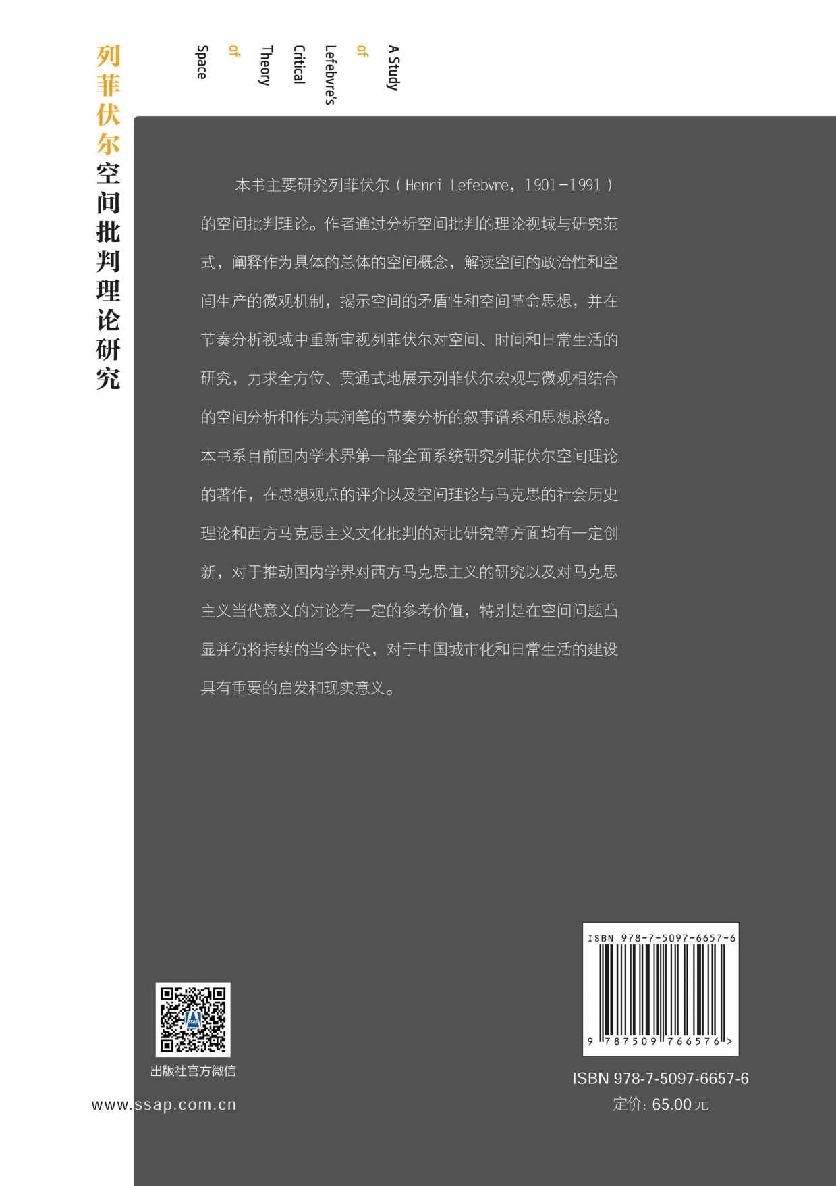
\includegraphics{images/00006.jpeg}
\end{figure}

\end{document}
